\documentclass[twoside]{book}

% Packages required by doxygen
\usepackage{fixltx2e}
\usepackage{calc}
\usepackage{doxygen}
\usepackage[export]{adjustbox} % also loads graphicx
\usepackage{graphicx}
\usepackage[utf8]{inputenc}
\usepackage{makeidx}
\usepackage{multicol}
\usepackage{multirow}
\PassOptionsToPackage{warn}{textcomp}
\usepackage{textcomp}
\usepackage[nointegrals]{wasysym}
\usepackage[table]{xcolor}

% Font selection
\usepackage[T1]{fontenc}
\usepackage[scaled=.90]{helvet}
\usepackage{courier}
\usepackage{amssymb}
\usepackage{sectsty}
\renewcommand{\familydefault}{\sfdefault}
\allsectionsfont{%
  \fontseries{bc}\selectfont%
  \color{darkgray}%
}
\renewcommand{\DoxyLabelFont}{%
  \fontseries{bc}\selectfont%
  \color{darkgray}%
}
\newcommand{\+}{\discretionary{\mbox{\scriptsize$\hookleftarrow$}}{}{}}

% Page & text layout
\usepackage{geometry}
\geometry{%
  a4paper,%
  top=2.5cm,%
  bottom=2.5cm,%
  left=2.5cm,%
  right=2.5cm%
}
\tolerance=750
\hfuzz=15pt
\hbadness=750
\setlength{\emergencystretch}{15pt}
\setlength{\parindent}{0cm}
\setlength{\parskip}{0.2cm}
\makeatletter
\renewcommand{\paragraph}{%
  \@startsection{paragraph}{4}{0ex}{-1.0ex}{1.0ex}{%
    \normalfont\normalsize\bfseries\SS@parafont%
  }%
}
\renewcommand{\subparagraph}{%
  \@startsection{subparagraph}{5}{0ex}{-1.0ex}{1.0ex}{%
    \normalfont\normalsize\bfseries\SS@subparafont%
  }%
}
\makeatother

% Headers & footers
\usepackage{fancyhdr}
\pagestyle{fancyplain}
\fancyhead[LE]{\fancyplain{}{\bfseries\thepage}}
\fancyhead[CE]{\fancyplain{}{}}
\fancyhead[RE]{\fancyplain{}{\bfseries\leftmark}}
\fancyhead[LO]{\fancyplain{}{\bfseries\rightmark}}
\fancyhead[CO]{\fancyplain{}{}}
\fancyhead[RO]{\fancyplain{}{\bfseries\thepage}}
\fancyfoot[LE]{\fancyplain{}{}}
\fancyfoot[CE]{\fancyplain{}{}}
\fancyfoot[RE]{\fancyplain{}{\bfseries\scriptsize Generated on Sun Jan 6 2019 01\+:20\+:39 for Bridges-\/\+Python-\/2.\+4 by Doxygen }}
\fancyfoot[LO]{\fancyplain{}{\bfseries\scriptsize Generated on Sun Jan 6 2019 01\+:20\+:39 for Bridges-\/\+Python-\/2.\+4 by Doxygen }}
\fancyfoot[CO]{\fancyplain{}{}}
\fancyfoot[RO]{\fancyplain{}{}}
\renewcommand{\footrulewidth}{0.4pt}
\renewcommand{\chaptermark}[1]{%
  \markboth{#1}{}%
}
\renewcommand{\sectionmark}[1]{%
  \markright{\thesection\ #1}%
}

% Indices & bibliography
\usepackage{natbib}
\usepackage[titles]{tocloft}
\setcounter{tocdepth}{3}
\setcounter{secnumdepth}{5}
\makeindex

% Hyperlinks (required, but should be loaded last)
\usepackage{ifpdf}
\ifpdf
  \usepackage[pdftex,pagebackref=true]{hyperref}
\else
  \usepackage[ps2pdf,pagebackref=true]{hyperref}
\fi
\hypersetup{%
  colorlinks=true,%
  linkcolor=blue,%
  citecolor=blue,%
  unicode%
}

% Custom commands
\newcommand{\clearemptydoublepage}{%
  \newpage{\pagestyle{empty}\cleardoublepage}%
}


%===== C O N T E N T S =====

\begin{document}

% Titlepage & ToC
\hypersetup{pageanchor=false,
             bookmarks=true,
             bookmarksnumbered=true,
             pdfencoding=unicode
            }
\pagenumbering{roman}
\begin{titlepage}
\vspace*{7cm}
\begin{center}%
{\Large Bridges-\/\+Python-\/2.4 \\[1ex]\large 2.\+4.\+0 }\\
\vspace*{1cm}
{\large Generated by Doxygen 1.8.10}\\
\vspace*{0.5cm}
{\small Sun Jan 6 2019 01:20:39}\\
\end{center}
\end{titlepage}
\clearemptydoublepage
\tableofcontents
\clearemptydoublepage
\pagenumbering{arabic}
\hypersetup{pageanchor=true}

%--- Begin generated contents ---
\chapter{Namespace Index}
\section{Namespace List}
Here is a list of all namespaces with brief descriptions\+:\begin{DoxyCompactList}
\item\contentsline{section}{\hyperlink{namespacebridges}{bridges} \\*This class can be used to create arrays of type Element$<$\+E$>$ where E is a generic type representation application specific data. Arrays are internally represented as 1\+D arrays; currently 1\+D, 2\+D and 3\+D arrays are supported }{\pageref{namespacebridges}}{}
\item\contentsline{section}{\hyperlink{namespacebridges_1_1base64}{bridges\+::base64} }{\pageref{namespacebridges_1_1base64}}{}
\item\contentsline{section}{\hyperlink{namespacebridges_1_1_j_s_o_n_util}{bridges\+::\+J\+S\+O\+N\+Util} }{\pageref{namespacebridges_1_1_j_s_o_n_util}}{}
\end{DoxyCompactList}

\chapter{Hierarchical Index}
\section{Class Hierarchy}
This inheritance list is sorted roughly, but not completely, alphabetically\+:\begin{DoxyCompactList}
\item \contentsline{section}{bridges\+:\+:dataset\+:\+:Actor\+Movie\+I\+M\+DB}{\pageref{classbridges_1_1dataset_1_1_actor_movie_i_m_d_b}}{}
\item \contentsline{section}{Audio\+Channel}{\pageref{class_audio_channel}}{}
\item \contentsline{section}{bridges\+:\+:dataset\+:\+:Book}{\pageref{classbridges_1_1dataset_1_1_book}}{}
\item \contentsline{section}{bridges\+:\+:datastructure\+:\+:Array3D$<$ E $>$\+:\+:Bracket\+\_\+helper}{\pageref{structbridges_1_1datastructure_1_1_array3_d_1_1_bracket__helper}}{}
\item \contentsline{section}{bridges\+:\+:datastructure\+:\+:Array2D$<$ E $>$\+:\+:Bracket\+\_\+helper}{\pageref{structbridges_1_1datastructure_1_1_array2_d_1_1_bracket__helper}}{}
\item \contentsline{section}{bridges\+:\+:datastructure\+:\+:Array3D$<$ E $>$\+:\+:Bracket\+\_\+helper2}{\pageref{structbridges_1_1datastructure_1_1_array3_d_1_1_bracket__helper2}}{}
\item \contentsline{section}{bridges\+:\+:datastructure\+:\+:Array3D$<$ E $>$\+:\+:Bracket\+\_\+helper2\+\_\+const}{\pageref{structbridges_1_1datastructure_1_1_array3_d_1_1_bracket__helper2__const}}{}
\item \contentsline{section}{bridges\+:\+:datastructure\+:\+:Array2D$<$ E $>$\+:\+:Bracket\+\_\+helper\+\_\+const}{\pageref{structbridges_1_1datastructure_1_1_array2_d_1_1_bracket__helper__const}}{}
\item \contentsline{section}{bridges\+:\+:datastructure\+:\+:Array3D$<$ E $>$\+:\+:Bracket\+\_\+helper\+\_\+const}{\pageref{structbridges_1_1datastructure_1_1_array3_d_1_1_bracket__helper__const}}{}
\item \contentsline{section}{bridges\+:\+:datastructure\+:\+:Grid$<$ E $>$\+:\+:Bracket\+Helper}{\pageref{classbridges_1_1datastructure_1_1_grid_1_1_bracket_helper}}{}
\item \contentsline{section}{bridges\+:\+:datastructure\+:\+:Grid$<$ E $>$\+:\+:Bracket\+Helper\+Const}{\pageref{classbridges_1_1datastructure_1_1_grid_1_1_bracket_helper_const}}{}
\item \contentsline{section}{bridges\+:\+:Bridges}{\pageref{classbridges_1_1_bridges}}{}
\item \contentsline{section}{bridges\+:\+:Cache}{\pageref{classbridges_1_1_cache}}{}
\begin{DoxyCompactList}
\item \contentsline{section}{bridges\+:\+:lru\+Cache}{\pageref{classbridges_1_1lru_cache}}{}
\item \contentsline{section}{bridges\+:\+:Simple\+Cache}{\pageref{classbridges_1_1_simple_cache}}{}
\end{DoxyCompactList}
\item \contentsline{section}{bridges\+:\+:dataset\+:\+:Cancer\+Incidence}{\pageref{classbridges_1_1dataset_1_1_cancer_incidence}}{}
\item \contentsline{section}{bridges\+:\+:datastructure\+:\+:Circ\+D\+Lelement$<$ E $>$\+:\+:Circ\+D\+Lelement\+\_\+constlisthelper}{\pageref{classbridges_1_1datastructure_1_1_circ_d_lelement_1_1_circ_d_lelement__constlisthelper}}{}
\item \contentsline{section}{bridges\+:\+:datastructure\+:\+:Circ\+D\+Lelement$<$ E $>$\+:\+:Circ\+D\+Lelement\+\_\+listhelper}{\pageref{classbridges_1_1datastructure_1_1_circ_d_lelement_1_1_circ_d_lelement__listhelper}}{}
\item \contentsline{section}{bridges\+:\+:datastructure\+:\+:Circ\+S\+Lelement$<$ E $>$\+:\+:Circ\+S\+Lelement\+\_\+constlisthelper}{\pageref{classbridges_1_1datastructure_1_1_circ_s_lelement_1_1_circ_s_lelement__constlisthelper}}{}
\item \contentsline{section}{bridges\+:\+:datastructure\+:\+:Circ\+S\+Lelement$<$ E $>$\+:\+:Circ\+S\+Lelement\+\_\+listhelper}{\pageref{classbridges_1_1datastructure_1_1_circ_s_lelement_1_1_circ_s_lelement__listhelper}}{}
\item \contentsline{section}{bridges\+:\+:datastructure\+:\+:Color}{\pageref{classbridges_1_1datastructure_1_1_color}}{}
\item \contentsline{section}{bridges\+:\+:datastructure\+:\+:Array1D$<$ E $>$\+:\+:const\+\_\+iterator}{\pageref{classbridges_1_1datastructure_1_1_array1_d_1_1const__iterator}}{}
\item \contentsline{section}{bridges\+:\+:datastructure\+:\+:Graph\+Adj\+List$<$ K, E1, E2 $>$\+:\+:Key\+Set\+\_\+helper\+:\+:const\+\_\+iterator}{\pageref{classbridges_1_1datastructure_1_1_graph_adj_list_1_1_key_set__helper_1_1const__iterator}}{}
\item \contentsline{section}{bridges\+:\+:datastructure\+:\+:Graph\+Adj\+List$<$ K, E1, E2 $>$\+:\+:Vertex\+Element\+Set\+\_\+listhelper\+:\+:const\+\_\+iterator}{\pageref{classbridges_1_1datastructure_1_1_graph_adj_list_1_1_vertex_element_set__listhelper_1_1const__iterator}}{}
\item \contentsline{section}{bridges\+:\+:datastructure\+:\+:Graph\+Adj\+List$<$ K, E1, E2 $>$\+:\+:const\+Vertex\+Element\+Set\+\_\+listhelper\+:\+:const\+\_\+iterator}{\pageref{classbridges_1_1datastructure_1_1_graph_adj_list_1_1const_vertex_element_set__listhelper_1_1const__iterator}}{}
\item \contentsline{section}{bridges\+:\+:datastructure\+:\+:Graph\+Adj\+List$<$ K, E1, E2 $>$\+:\+:const\+Vertex\+Element\+Set\+\_\+listhelper}{\pageref{classbridges_1_1datastructure_1_1_graph_adj_list_1_1const_vertex_element_set__listhelper}}{}
\item \contentsline{section}{bridges\+:\+:Data\+Source}{\pageref{classbridges_1_1_data_source}}{}
\item \contentsline{section}{bridges\+:\+:datastructure\+:\+:Data\+Structure}{\pageref{classbridges_1_1datastructure_1_1_data_structure}}{}
\begin{DoxyCompactList}
\item \contentsline{section}{bridges\+:\+:datastructure\+:\+:Array$<$ E $>$}{\pageref{classbridges_1_1datastructure_1_1_array}}{}
\begin{DoxyCompactList}
\item \contentsline{section}{bridges\+:\+:datastructure\+:\+:Array1D$<$ E $>$}{\pageref{classbridges_1_1datastructure_1_1_array1_d}}{}
\item \contentsline{section}{bridges\+:\+:datastructure\+:\+:Array2D$<$ E $>$}{\pageref{classbridges_1_1datastructure_1_1_array2_d}}{}
\item \contentsline{section}{bridges\+:\+:datastructure\+:\+:Array3D$<$ E $>$}{\pageref{classbridges_1_1datastructure_1_1_array3_d}}{}
\end{DoxyCompactList}
\item \contentsline{section}{bridges\+:\+:datastructure\+:\+:Audio\+Clip}{\pageref{classbridges_1_1datastructure_1_1_audio_clip}}{}
\item \contentsline{section}{bridges\+:\+:datastructure\+:\+:Element\+Array$<$ E, X, Y, Z $>$}{\pageref{classbridges_1_1datastructure_1_1_element_array}}{}
\item \contentsline{section}{bridges\+:\+:datastructure\+:\+:Graph\+Adj\+List$<$ K, E1, E2 $>$}{\pageref{classbridges_1_1datastructure_1_1_graph_adj_list}}{}
\item \contentsline{section}{bridges\+:\+:datastructure\+:\+:Graph\+Adj\+Matrix$<$ K, E1, E2 $>$}{\pageref{classbridges_1_1datastructure_1_1_graph_adj_matrix}}{}
\item \contentsline{section}{bridges\+:\+:datastructure\+:\+:Grid$<$ E $>$}{\pageref{classbridges_1_1datastructure_1_1_grid}}{}
\item \contentsline{section}{bridges\+:\+:datastructure\+:\+:Line\+Chart}{\pageref{classbridges_1_1datastructure_1_1_line_chart}}{}
\item \contentsline{section}{bridges\+:\+:datastructure\+:\+:S\+Lelement$<$ E $>$}{\pageref{classbridges_1_1datastructure_1_1_s_lelement}}{}
\begin{DoxyCompactList}
\item \contentsline{section}{bridges\+:\+:datastructure\+:\+:Circ\+S\+Lelement$<$ E $>$}{\pageref{classbridges_1_1datastructure_1_1_circ_s_lelement}}{}
\item \contentsline{section}{bridges\+:\+:datastructure\+:\+:D\+Lelement$<$ E $>$}{\pageref{classbridges_1_1datastructure_1_1_d_lelement}}{}
\begin{DoxyCompactList}
\item \contentsline{section}{bridges\+:\+:datastructure\+:\+:Circ\+D\+Lelement$<$ E $>$}{\pageref{classbridges_1_1datastructure_1_1_circ_d_lelement}}{}
\end{DoxyCompactList}
\item \contentsline{section}{bridges\+:\+:datastructure\+:\+:M\+Lelement$<$ E $>$}{\pageref{classbridges_1_1datastructure_1_1_m_lelement}}{}
\end{DoxyCompactList}
\item \contentsline{section}{bridges\+:\+:datastructure\+:\+:Symbol\+Collection}{\pageref{classbridges_1_1datastructure_1_1_symbol_collection}}{}
\item \contentsline{section}{bridges\+:\+:datastructure\+:\+:Tree\+Element$<$ E $>$}{\pageref{classbridges_1_1datastructure_1_1_tree_element}}{}
\begin{DoxyCompactList}
\item \contentsline{section}{bridges\+:\+:datastructure\+:\+:Bin\+Tree\+Element$<$ E $>$}{\pageref{classbridges_1_1datastructure_1_1_bin_tree_element}}{}
\begin{DoxyCompactList}
\item \contentsline{section}{bridges\+:\+:datastructure\+:\+:B\+S\+T\+Element$<$ K, E $>$}{\pageref{classbridges_1_1datastructure_1_1_b_s_t_element}}{}
\begin{DoxyCompactList}
\item \contentsline{section}{bridges\+:\+:datastructure\+:\+:A\+V\+L\+Tree\+Element$<$ K, E $>$}{\pageref{classbridges_1_1datastructure_1_1_a_v_l_tree_element}}{}
\item \contentsline{section}{bridges\+:\+:datastructure\+:\+:Kd\+Tree\+Element$<$ K, E $>$}{\pageref{classbridges_1_1datastructure_1_1_kd_tree_element}}{}
\end{DoxyCompactList}
\end{DoxyCompactList}
\item \contentsline{section}{bridges\+:\+:datastructure\+:\+:B\+T\+Element$<$ E $>$}{\pageref{classbridges_1_1datastructure_1_1_b_t_element}}{}
\end{DoxyCompactList}
\item \contentsline{section}{bridges\+:\+:datastructure\+:\+:Grid$<$ Color $>$}{\pageref{classbridges_1_1datastructure_1_1_grid}}{}
\begin{DoxyCompactList}
\item \contentsline{section}{bridges\+:\+:datastructure\+:\+:Color\+Grid}{\pageref{classbridges_1_1datastructure_1_1_color_grid}}{}
\end{DoxyCompactList}
\item \contentsline{section}{bridges\+:\+:datastructure\+:\+:Grid$<$ Game\+Cell $>$}{\pageref{classbridges_1_1datastructure_1_1_grid}}{}
\begin{DoxyCompactList}
\item \contentsline{section}{bridges\+:\+:game\+:\+:Game\+Grid}{\pageref{classbridges_1_1game_1_1_game_grid}}{}
\end{DoxyCompactList}
\item \contentsline{section}{bridges\+:\+:datastructure\+:\+:S\+Lelement$<$ bridges\+:\+:datastructure\+:\+:Edge$<$ K, E2 $>$ $>$}{\pageref{classbridges_1_1datastructure_1_1_s_lelement}}{}
\end{DoxyCompactList}
\item \contentsline{section}{bridges\+:\+:datastructure\+:\+:D\+Lelement$<$ E $>$\+:\+:D\+Lelement\+\_\+constlisthelper}{\pageref{classbridges_1_1datastructure_1_1_d_lelement_1_1_d_lelement__constlisthelper}}{}
\item \contentsline{section}{bridges\+:\+:datastructure\+:\+:D\+Lelement$<$ E $>$\+:\+:D\+Lelement\+\_\+listhelper}{\pageref{classbridges_1_1datastructure_1_1_d_lelement_1_1_d_lelement__listhelper}}{}
\item \contentsline{section}{bridges\+:\+:dataset\+:\+:Earthquake\+U\+S\+GS}{\pageref{classbridges_1_1dataset_1_1_earthquake_u_s_g_s}}{}
\item \contentsline{section}{bridges\+:\+:datastructure\+:\+:Edge$<$ K, E2 $>$}{\pageref{classbridges_1_1datastructure_1_1_edge}}{}
\item \contentsline{section}{bridges\+:\+:datastructure\+:\+:Element$<$ E $>$}{\pageref{classbridges_1_1datastructure_1_1_element}}{}
\begin{DoxyCompactList}
\item \contentsline{section}{bridges\+:\+:datastructure\+:\+:S\+Lelement$<$ E $>$}{\pageref{classbridges_1_1datastructure_1_1_s_lelement}}{}
\item \contentsline{section}{bridges\+:\+:datastructure\+:\+:Tree\+Element$<$ E $>$}{\pageref{classbridges_1_1datastructure_1_1_tree_element}}{}
\end{DoxyCompactList}
\item \contentsline{section}{bridges\+:\+:datastructure\+:\+:Element$<$ bridges\+:\+:datastructure\+:\+:Edge$<$ K, E2 $>$ $>$}{\pageref{classbridges_1_1datastructure_1_1_element}}{}
\begin{DoxyCompactList}
\item \contentsline{section}{bridges\+:\+:datastructure\+:\+:S\+Lelement$<$ bridges\+:\+:datastructure\+:\+:Edge$<$ K, E2 $>$ $>$}{\pageref{classbridges_1_1datastructure_1_1_s_lelement}}{}
\end{DoxyCompactList}
\item \contentsline{section}{bridges\+:\+:datastructure\+:\+:Element$<$ E1 $>$}{\pageref{classbridges_1_1datastructure_1_1_element}}{}
\item \contentsline{section}{bridges\+:\+:datastructure\+:\+:Element\+Visualizer}{\pageref{classbridges_1_1datastructure_1_1_element_visualizer}}{}
\item \contentsline{section}{bridges\+:\+:dataset\+:\+:Elevation\+Data}{\pageref{classbridges_1_1dataset_1_1_elevation_data}}{}
\item std\+:\+:exception\begin{DoxyCompactList}
\item \contentsline{section}{bridges\+:\+:Cache\+Exception}{\pageref{classbridges_1_1_cache_exception}}{}
\end{DoxyCompactList}
\item \contentsline{section}{bridges\+:\+:dataset\+:\+:Game}{\pageref{classbridges_1_1dataset_1_1_game}}{}
\item \contentsline{section}{bridges\+:\+:game\+:\+:Game\+Base}{\pageref{classbridges_1_1game_1_1_game_base}}{}
\begin{DoxyCompactList}
\item \contentsline{section}{bridges\+:\+:game\+:\+:Non\+Blocking\+Game}{\pageref{classbridges_1_1game_1_1_non_blocking_game}}{}
\end{DoxyCompactList}
\item \contentsline{section}{bridges\+:\+:game\+:\+:Game\+Cell}{\pageref{classbridges_1_1game_1_1_game_cell}}{}
\item \contentsline{section}{bridges\+:\+:benchmark\+:\+:Graph\+Benchmark}{\pageref{classbridges_1_1benchmark_1_1_graph_benchmark}}{}
\begin{DoxyCompactList}
\item \contentsline{section}{bridges\+:\+:benchmark\+:\+:B\+F\+S\+Benchmark}{\pageref{classbridges_1_1benchmark_1_1_b_f_s_benchmark}}{}
\item \contentsline{section}{bridges\+:\+:benchmark\+:\+:Page\+Rank\+Benchmark}{\pageref{classbridges_1_1benchmark_1_1_page_rank_benchmark}}{}
\item \contentsline{section}{bridges\+:\+:benchmark\+:\+:Shortest\+Path\+Benchmark}{\pageref{classbridges_1_1benchmark_1_1_shortest_path_benchmark}}{}
\end{DoxyCompactList}
\item \contentsline{section}{bridges\+:\+:dataset\+:\+:Gutenberg\+Book}{\pageref{classbridges_1_1dataset_1_1_gutenberg_book}}{}
\item \contentsline{section}{bridges\+:\+:datastructure\+:\+:Array1D$<$ E $>$\+:\+:iterator}{\pageref{classbridges_1_1datastructure_1_1_array1_d_1_1iterator}}{}
\item \contentsline{section}{bridges\+:\+:datastructure\+:\+:Circ\+D\+Lelement$<$ E $>$\+:\+:Circ\+D\+Lelement\+\_\+listhelper\+:\+:iterator}{\pageref{classbridges_1_1datastructure_1_1_circ_d_lelement_1_1_circ_d_lelement__listhelper_1_1iterator}}{}
\item \contentsline{section}{bridges\+:\+:datastructure\+:\+:Circ\+D\+Lelement$<$ E $>$\+:\+:Circ\+D\+Lelement\+\_\+constlisthelper\+:\+:iterator}{\pageref{classbridges_1_1datastructure_1_1_circ_d_lelement_1_1_circ_d_lelement__constlisthelper_1_1iterator}}{}
\item \contentsline{section}{bridges\+:\+:datastructure\+:\+:Circ\+S\+Lelement$<$ E $>$\+:\+:Circ\+S\+Lelement\+\_\+listhelper\+:\+:iterator}{\pageref{classbridges_1_1datastructure_1_1_circ_s_lelement_1_1_circ_s_lelement__listhelper_1_1iterator}}{}
\item \contentsline{section}{bridges\+:\+:datastructure\+:\+:Circ\+S\+Lelement$<$ E $>$\+:\+:Circ\+S\+Lelement\+\_\+constlisthelper\+:\+:iterator}{\pageref{classbridges_1_1datastructure_1_1_circ_s_lelement_1_1_circ_s_lelement__constlisthelper_1_1iterator}}{}
\item \contentsline{section}{bridges\+:\+:datastructure\+:\+:D\+Lelement$<$ E $>$\+:\+:D\+Lelement\+\_\+listhelper\+:\+:iterator}{\pageref{classbridges_1_1datastructure_1_1_d_lelement_1_1_d_lelement__listhelper_1_1iterator}}{}
\item \contentsline{section}{bridges\+:\+:datastructure\+:\+:Graph\+Adj\+List$<$ K, E1, E2 $>$\+:\+:Vertex\+Element\+Set\+\_\+listhelper\+:\+:iterator}{\pageref{classbridges_1_1datastructure_1_1_graph_adj_list_1_1_vertex_element_set__listhelper_1_1iterator}}{}
\item \contentsline{section}{bridges\+:\+:datastructure\+:\+:D\+Lelement$<$ E $>$\+:\+:D\+Lelement\+\_\+constlisthelper\+:\+:iterator}{\pageref{classbridges_1_1datastructure_1_1_d_lelement_1_1_d_lelement__constlisthelper_1_1iterator}}{}
\item \contentsline{section}{bridges\+:\+:datastructure\+:\+:S\+Lelement$<$ E $>$\+:\+:S\+Lelement\+\_\+listhelper\+:\+:iterator}{\pageref{classbridges_1_1datastructure_1_1_s_lelement_1_1_s_lelement__listhelper_1_1iterator}}{}
\item \contentsline{section}{bridges\+:\+:datastructure\+:\+:S\+Lelement$<$ E $>$\+:\+:S\+Lelement\+\_\+constlisthelper\+:\+:iterator}{\pageref{classbridges_1_1datastructure_1_1_s_lelement_1_1_s_lelement__constlisthelper_1_1iterator}}{}
\item \contentsline{section}{bridges\+:\+:game\+:\+:Keypress\+Listener}{\pageref{classbridges_1_1game_1_1_keypress_listener}}{}
\begin{DoxyCompactList}
\item \contentsline{section}{bridges\+:\+:game\+:\+:Input\+Helper}{\pageref{classbridges_1_1game_1_1_input_helper}}{}
\end{DoxyCompactList}
\item \contentsline{section}{bridges\+:\+:datastructure\+:\+:Graph\+Adj\+List$<$ K, E1, E2 $>$\+:\+:Key\+Set\+\_\+helper}{\pageref{classbridges_1_1datastructure_1_1_graph_adj_list_1_1_key_set__helper}}{}
\item \contentsline{section}{bridges\+:\+:datastructure\+:\+:Link\+Visualizer}{\pageref{classbridges_1_1datastructure_1_1_link_visualizer}}{}
\item \contentsline{section}{bridges\+:\+:dataset\+:\+:Movie\+Actor\+Wikidata}{\pageref{classbridges_1_1dataset_1_1_movie_actor_wikidata}}{}
\item \contentsline{section}{bridges\+:\+:dataset\+:\+:O\+S\+M\+Data}{\pageref{classbridges_1_1dataset_1_1_o_s_m_data}}{}
\item \contentsline{section}{bridges\+:\+:dataset\+:\+:O\+S\+M\+Edge}{\pageref{classbridges_1_1dataset_1_1_o_s_m_edge}}{}
\item \contentsline{section}{bridges\+:\+:dataset\+:\+:O\+S\+M\+Vertex}{\pageref{classbridges_1_1dataset_1_1_o_s_m_vertex}}{}
\item \contentsline{section}{rapidjson\+\_\+exception}{\pageref{structrapidjson__exception}}{}
\item \contentsline{section}{bridges\+:\+:Server\+Comm}{\pageref{classbridges_1_1_server_comm}}{}
\item \contentsline{section}{bridges\+:\+:dataset\+:\+:Shakespeare}{\pageref{classbridges_1_1dataset_1_1_shakespeare}}{}
\item \contentsline{section}{bridges\+:\+:datastructure\+:\+:S\+Lelement$<$ E $>$\+:\+:S\+Lelement\+\_\+constlisthelper}{\pageref{classbridges_1_1datastructure_1_1_s_lelement_1_1_s_lelement__constlisthelper}}{}
\item \contentsline{section}{bridges\+:\+:datastructure\+:\+:S\+Lelement$<$ E $>$\+:\+:S\+Lelement\+\_\+listhelper}{\pageref{classbridges_1_1datastructure_1_1_s_lelement_1_1_s_lelement__listhelper}}{}
\item \contentsline{section}{bridges\+:\+:game\+:\+:Socket\+Connection}{\pageref{classbridges_1_1game_1_1_socket_connection}}{}
\item \contentsline{section}{bridges\+:\+:dataset\+:\+:Song}{\pageref{classbridges_1_1dataset_1_1_song}}{}
\item \contentsline{section}{bridges\+:\+:benchmark\+:\+:Sorting\+Benchmark}{\pageref{classbridges_1_1benchmark_1_1_sorting_benchmark}}{}
\item \contentsline{section}{bridges\+:\+:datastructure\+:\+:Symbol}{\pageref{classbridges_1_1datastructure_1_1_symbol}}{}
\begin{DoxyCompactList}
\item \contentsline{section}{bridges\+:\+:datastructure\+:\+:Circle}{\pageref{classbridges_1_1datastructure_1_1_circle}}{}
\item \contentsline{section}{bridges\+:\+:datastructure\+:\+:Label}{\pageref{classbridges_1_1datastructure_1_1_label}}{}
\item \contentsline{section}{bridges\+:\+:datastructure\+:\+:Polyline}{\pageref{classbridges_1_1datastructure_1_1_polyline}}{}
\begin{DoxyCompactList}
\item \contentsline{section}{bridges\+:\+:datastructure\+:\+:Polygon}{\pageref{classbridges_1_1datastructure_1_1_polygon}}{}
\end{DoxyCompactList}
\item \contentsline{section}{bridges\+:\+:datastructure\+:\+:Rectangle}{\pageref{classbridges_1_1datastructure_1_1_rectangle}}{}
\end{DoxyCompactList}
\item \contentsline{section}{bridges\+:\+:datastructure\+:\+:Graph\+Adj\+List$<$ K, E1, E2 $>$\+:\+:Vertex\+Element\+Set\+\_\+listhelper}{\pageref{classbridges_1_1datastructure_1_1_graph_adj_list_1_1_vertex_element_set__listhelper}}{}
\item \contentsline{section}{bridges\+:\+:Wave\+Header}{\pageref{structbridges_1_1_wave_header}}{}
\end{DoxyCompactList}

\chapter{Class Index}
\section{Class List}
Here are the classes, structs, unions and interfaces with brief descriptions\+:\begin{DoxyCompactList}
\item\contentsline{section}{\mbox{\hyperlink{classbridges_1_1data__src__dependent_1_1_actor}{bridges.\+data\+\_\+src\+\_\+dependent.\+Actor}} }{\pageref{classbridges_1_1data__src__dependent_1_1_actor}}{}
\item\contentsline{section}{\mbox{\hyperlink{classbridges_1_1data__src__dependent_1_1_actor_movie_i_m_d_b}{bridges.\+data\+\_\+src\+\_\+dependent.\+Actor\+Movie\+I\+M\+DB}} \\*This class can be used to work with \mbox{\hyperlink{classbridges_1_1data__src__dependent_1_1_i_m_d_b}{I\+M\+DB}} actor movie data }{\pageref{classbridges_1_1data__src__dependent_1_1_actor_movie_i_m_d_b}}{}
\item\contentsline{section}{\mbox{\hyperlink{classbridges_1_1base_1_1_array}{bridges.\+base.\+Array$<$ E $>$}} \\*This class can be used to create arrays of type Element$<$\+E$>$ }{\pageref{classbridges_1_1base_1_1_array}}{}
\item\contentsline{section}{\mbox{\hyperlink{classbridges_1_1base_1_1_array_element}{bridges.\+base.\+Array\+Element$<$ E $>$}} }{\pageref{classbridges_1_1base_1_1_array_element}}{}
\item\contentsline{section}{\mbox{\hyperlink{classbridges_1_1base_1_1_array_of_element}{bridges.\+base.\+Array\+Of\+Element$<$ E extends Comparable$<$? super E $>$}} }{\pageref{classbridges_1_1base_1_1_array_of_element}}{}
\item\contentsline{section}{\mbox{\hyperlink{classbridges_1_1base_1_1_a_v_l_tree_element}{bridges.\+base.\+A\+V\+L\+Tree\+Element$<$ K, E $>$}} \\*This class extends the \mbox{\hyperlink{classbridges_1_1base_1_1_b_s_t_element}{B\+S\+T\+Element}} class by adding a height and balance factor fields that are useful in A\+VL trees }{\pageref{classbridges_1_1base_1_1_a_v_l_tree_element}}{}
\item\contentsline{section}{\mbox{\hyperlink{classbridges_1_1base_1_1_bin_tree_element}{bridges.\+base.\+Bin\+Tree\+Element$<$ E $>$}} \\*This class is extended from the \mbox{\hyperlink{classbridges_1_1base_1_1_tree_element}{Tree\+Element}} class and can be used to create binary tree element objects }{\pageref{classbridges_1_1base_1_1_bin_tree_element}}{}
\item\contentsline{section}{\mbox{\hyperlink{classbridges_1_1connect_1_1_bridges}{bridges.\+connect.\+Bridges}} \\*The \mbox{\hyperlink{classbridges_1_1connect_1_1_bridges}{Bridges}} class is the main class that provides interfaces to datasets, maintains user and assignment information, and connects to the \mbox{\hyperlink{classbridges_1_1connect_1_1_bridges}{Bridges}} server }{\pageref{classbridges_1_1connect_1_1_bridges}}{}
\item\contentsline{section}{\mbox{\hyperlink{classbridges_1_1base_1_1_b_s_t_element}{bridges.\+base.\+B\+S\+T\+Element$<$ K, E $>$}} \\*The \mbox{\hyperlink{classbridges_1_1base_1_1_b_s_t_element}{B\+S\+T\+Element}} class is the building block for creating binary search trees }{\pageref{classbridges_1_1base_1_1_b_s_t_element}}{}
\item\contentsline{section}{\mbox{\hyperlink{classbridges_1_1data__src__dependent_1_1_cancer_incidence}{bridges.\+data\+\_\+src\+\_\+dependent.\+Cancer\+Incidence}} \\*This is a helper class to work with Cancer Incidence data from C\+DC }{\pageref{classbridges_1_1data__src__dependent_1_1_cancer_incidence}}{}
\item\contentsline{section}{\mbox{\hyperlink{classbridges_1_1base_1_1_circ_d_lelement}{bridges.\+base.\+Circ\+D\+Lelement$<$ E $>$}} \\*This class can be used to instantiate Circular Doubly Linked List Elements }{\pageref{classbridges_1_1base_1_1_circ_d_lelement}}{}
\item\contentsline{section}{\mbox{\hyperlink{classbridges_1_1base_1_1_circ_s_lelement}{bridges.\+base.\+Circ\+S\+Lelement$<$ E $>$}} \\*This class can be used to instantiate Singly Linked Circular List Elements }{\pageref{classbridges_1_1base_1_1_circ_s_lelement}}{}
\item\contentsline{section}{\mbox{\hyperlink{classbridges_1_1base_1_1_color}{bridges.\+base.\+Color}} \\*This class is used to represent colors in B\+R\+I\+D\+G\+ES }{\pageref{classbridges_1_1base_1_1_color}}{}
\item\contentsline{section}{\mbox{\hyperlink{classbridges_1_1base_1_1_color_grid}{bridges.\+base.\+Color\+Grid}} \\*This is a class in B\+R\+I\+D\+G\+ES for representing an (n x n) grid }{\pageref{classbridges_1_1base_1_1_color_grid}}{}
\item\contentsline{section}{\mbox{\hyperlink{classbridges_1_1connect_1_1_connector}{bridges.\+connect.\+Connector}} \\*This class provides interfaces to the B\+R\+I\+D\+G\+ES server, J\+S\+ON processing, etc }{\pageref{classbridges_1_1connect_1_1_connector}}{}
\item\contentsline{section}{\mbox{\hyperlink{classbridges_1_1connect_1_1_data_formatter}{bridges.\+connect.\+Data\+Formatter}} \\*This class provides interfaces to all data sources supported by B\+R\+I\+D\+G\+ES }{\pageref{classbridges_1_1connect_1_1_data_formatter}}{}
\item\contentsline{section}{\mbox{\hyperlink{classbridges_1_1validation_1_1_data_formatter_exception}{bridges.\+validation.\+Data\+Formatter\+Exception}} }{\pageref{classbridges_1_1validation_1_1_data_formatter_exception}}{}
\item\contentsline{section}{\mbox{\hyperlink{classbridges_1_1base_1_1_data_struct}{bridges.\+base.\+Data\+Struct}} \\*This is an abstract super class that is extended by all Bridges subclasses and provides some methods that are used universally across B\+R\+I\+D\+G\+ES }{\pageref{classbridges_1_1base_1_1_data_struct}}{}
\item\contentsline{section}{\mbox{\hyperlink{classbridges_1_1base_1_1_d_lelement}{bridges.\+base.\+D\+Lelement$<$ E $>$}} \\*This class is used to create doubly linked element objects }{\pageref{classbridges_1_1base_1_1_d_lelement}}{}
\item\contentsline{section}{\mbox{\hyperlink{classbridges_1_1data__src__dependent_1_1_earthquake_u_s_g_s}{bridges.\+data\+\_\+src\+\_\+dependent.\+Earthquake\+U\+S\+GS}} }{\pageref{classbridges_1_1data__src__dependent_1_1_earthquake_u_s_g_s}}{}
\item\contentsline{section}{\mbox{\hyperlink{classbridges_1_1base_1_1_edge}{bridges.\+base.\+Edge$<$ K, E2 $>$}} \\*This class is used to represent the edges in a graph and will appear as links in the B\+R\+I\+D\+G\+ES graph visualization }{\pageref{classbridges_1_1base_1_1_edge}}{}
\item\contentsline{section}{\mbox{\hyperlink{classbridges_1_1base_1_1_element}{bridges.\+base.\+Element$<$ E $>$}} \\*This is the main superclass in B\+R\+I\+D\+G\+ES for deriving a number of objects used in building arrays, lists, trees and graph data structures }{\pageref{classbridges_1_1base_1_1_element}}{}
\item\contentsline{section}{\mbox{\hyperlink{classbridges_1_1base_1_1_element_visualizer}{bridges.\+base.\+Element\+Visualizer}} \\*This class maintains the visual attributes of each B\+R\+I\+D\+G\+ES element }{\pageref{classbridges_1_1base_1_1_element_visualizer}}{}
\item\contentsline{section}{\mbox{\hyperlink{classbridges_1_1data__src__dependent_1_1_follower}{bridges.\+data\+\_\+src\+\_\+dependent.\+Follower}} }{\pageref{classbridges_1_1data__src__dependent_1_1_follower}}{}
\item\contentsline{section}{\mbox{\hyperlink{classbridges_1_1data__src__dependent_1_1_game}{bridges.\+data\+\_\+src\+\_\+dependent.\+Game}} \\*A \mbox{\hyperlink{classbridges_1_1data__src__dependent_1_1_game}{Game}} object, used along with the Games data source }{\pageref{classbridges_1_1data__src__dependent_1_1_game}}{}
\item\contentsline{section}{\mbox{\hyperlink{classbridges_1_1base_1_1_graph_adj_list}{bridges.\+base.\+Graph\+Adj\+List$<$ K, E1, E2 $>$}} \\*The \mbox{\hyperlink{classbridges_1_1base_1_1_graph_adj_list}{Graph\+Adj\+List}} class can be used to represent adjacency list based graphs in B\+R\+I\+D\+G\+ES }{\pageref{classbridges_1_1base_1_1_graph_adj_list}}{}
\item\contentsline{section}{\mbox{\hyperlink{classbridges_1_1base_1_1_graph_adj_list_simple}{bridges.\+base.\+Graph\+Adj\+List\+Simple$<$ K $>$}} \\*The \mbox{\hyperlink{classbridges_1_1base_1_1_graph_adj_list_simple}{Graph\+Adj\+List\+Simple}} class is a simplification of the \mbox{\hyperlink{classbridges_1_1base_1_1_graph_adj_list}{Graph\+Adj\+List}} class; this class is useful in applications where vertex and edge specific information is not used; this class is thus a specialization of \mbox{\hyperlink{classbridges_1_1base_1_1_graph_adj_list}{Graph\+Adj\+List}} with only a single generic parameter that specifies the key type }{\pageref{classbridges_1_1base_1_1_graph_adj_list_simple}}{}
\item\contentsline{section}{\mbox{\hyperlink{classbridges_1_1base_1_1_graph_adj_matrix}{bridges.\+base.\+Graph\+Adj\+Matrix$<$ K, E1, E2 $>$}} \\*The \mbox{\hyperlink{classbridges_1_1base_1_1_graph_adj_matrix}{Graph\+Adj\+Matrix}} class can be used to represent adjacency matrix based graphs in B\+R\+I\+D\+G\+ES }{\pageref{classbridges_1_1base_1_1_graph_adj_matrix}}{}
\item\contentsline{section}{\mbox{\hyperlink{classbridges_1_1base_1_1_graph_adj_matrix_simple}{bridges.\+base.\+Graph\+Adj\+Matrix\+Simple$<$ K $>$}} \\*The \mbox{\hyperlink{classbridges_1_1base_1_1_graph_adj_matrix_simple}{Graph\+Adj\+Matrix\+Simple}} class is a simplification of the \mbox{\hyperlink{classbridges_1_1base_1_1_graph_adj_matrix}{Graph\+Adj\+Matrix}} class; this class is useful in applications where vertex and edge specific information is not used; this class is thus a specialization of \mbox{\hyperlink{classbridges_1_1base_1_1_graph_adj_list}{Graph\+Adj\+List}} with only a single generic parameter that specifies the key type }{\pageref{classbridges_1_1base_1_1_graph_adj_matrix_simple}}{}
\item\contentsline{section}{\mbox{\hyperlink{classbridges_1_1base_1_1_grid}{bridges.\+base.\+Grid$<$ E $>$}} \\*This is a class in B\+R\+I\+D\+G\+ES for representing an (n x n) grid }{\pageref{classbridges_1_1base_1_1_grid}}{}
\item\contentsline{section}{\mbox{\hyperlink{classbridges_1_1data__src__dependent_1_1_gutenberg_book}{bridges.\+data\+\_\+src\+\_\+dependent.\+Gutenberg\+Book}} \\*A Gutenberg Book object, used along with the Gutenberg books data source (\href{https://www.gutenberg.org/}{\tt https\+://www.\+gutenberg.\+org/}) }{\pageref{classbridges_1_1data__src__dependent_1_1_gutenberg_book}}{}
\item\contentsline{section}{\mbox{\hyperlink{classbridges_1_1data__src__dependent_1_1_i_m_d_b}{bridges.\+data\+\_\+src\+\_\+dependent.\+I\+M\+DB}} }{\pageref{classbridges_1_1data__src__dependent_1_1_i_m_d_b}}{}
\item\contentsline{section}{\mbox{\hyperlink{classbridges_1_1validation_1_1_invalid_value_exception}{bridges.\+validation.\+Invalid\+Value\+Exception}} }{\pageref{classbridges_1_1validation_1_1_invalid_value_exception}}{}
\item\contentsline{section}{\mbox{\hyperlink{classbridges_1_1base_1_1_link_visualizer}{bridges.\+base.\+Link\+Visualizer}} \\*This class maintains the visual attributes of links that join Bridges elements }{\pageref{classbridges_1_1base_1_1_link_visualizer}}{}
\item\contentsline{section}{\mbox{\hyperlink{classbridges_1_1base_1_1_m_lelement}{bridges.\+base.\+M\+Lelement$<$ E $>$}} \\*This class can be used to instantiate Multi-\/list Elements }{\pageref{classbridges_1_1base_1_1_m_lelement}}{}
\item\contentsline{section}{\mbox{\hyperlink{classbridges_1_1data__src__dependent_1_1_movie}{bridges.\+data\+\_\+src\+\_\+dependent.\+Movie}} }{\pageref{classbridges_1_1data__src__dependent_1_1_movie}}{}
\item\contentsline{section}{\mbox{\hyperlink{classbridges_1_1validation_1_1_output_log}{bridges.\+validation.\+Output\+Log}} }{\pageref{classbridges_1_1validation_1_1_output_log}}{}
\item\contentsline{section}{\mbox{\hyperlink{classbridges_1_1validation_1_1_rate_limit_exception}{bridges.\+validation.\+Rate\+Limit\+Exception}} }{\pageref{classbridges_1_1validation_1_1_rate_limit_exception}}{}
\item\contentsline{section}{\mbox{\hyperlink{classbridges_1_1data__src__dependent_1_1_rotten_tomatos}{bridges.\+data\+\_\+src\+\_\+dependent.\+Rotten\+Tomatos}} }{\pageref{classbridges_1_1data__src__dependent_1_1_rotten_tomatos}}{}
\item\contentsline{section}{\mbox{\hyperlink{classbridges_1_1data__src__dependent_1_1_sample_data_generator}{bridges.\+data\+\_\+src\+\_\+dependent.\+Sample\+Data\+Generator}} }{\pageref{classbridges_1_1data__src__dependent_1_1_sample_data_generator}}{}
\item\contentsline{section}{\mbox{\hyperlink{classbridges_1_1data__src__dependent_1_1_shakespeare}{bridges.\+data\+\_\+src\+\_\+dependent.\+Shakespeare}} \\*A \mbox{\hyperlink{classbridges_1_1data__src__dependent_1_1_shakespeare}{Shakespeare}} Data source object containing sonnets, poems and plays }{\pageref{classbridges_1_1data__src__dependent_1_1_shakespeare}}{}
\item\contentsline{section}{\mbox{\hyperlink{classbridges_1_1base_1_1_s_lelement}{bridges.\+base.\+S\+Lelement$<$ E $>$}} \\*This class can be used to instantiate Singly Linked Elements }{\pageref{classbridges_1_1base_1_1_s_lelement}}{}
\item\contentsline{section}{\mbox{\hyperlink{classbridges_1_1data__src__dependent_1_1_song}{bridges.\+data\+\_\+src\+\_\+dependent.\+Song}} \\*A \mbox{\hyperlink{classbridges_1_1data__src__dependent_1_1_song}{Song}} object, used along with the Songs data source (using the Genius A\+PI }{\pageref{classbridges_1_1data__src__dependent_1_1_song}}{}
\item\contentsline{section}{\mbox{\hyperlink{classbridges_1_1base_1_1_tree_element}{bridges.\+base.\+Tree\+Element$<$ E $>$}} \\*This class extends \mbox{\hyperlink{classbridges_1_1base_1_1_element}{Element}} to represent general trees with arbitrary number of children }{\pageref{classbridges_1_1base_1_1_tree_element}}{}
\item\contentsline{section}{\mbox{\hyperlink{classbridges_1_1data__src__dependent_1_1_tweet}{bridges.\+data\+\_\+src\+\_\+dependent.\+Tweet}} }{\pageref{classbridges_1_1data__src__dependent_1_1_tweet}}{}
\item\contentsline{section}{\mbox{\hyperlink{classbridges_1_1data__src__dependent_1_1_twitter}{bridges.\+data\+\_\+src\+\_\+dependent.\+Twitter}} }{\pageref{classbridges_1_1data__src__dependent_1_1_twitter}}{}
\item\contentsline{section}{\mbox{\hyperlink{classbridges_1_1data__src__dependent_1_1_twitter_account}{bridges.\+data\+\_\+src\+\_\+dependent.\+Twitter\+Account}} }{\pageref{classbridges_1_1data__src__dependent_1_1_twitter_account}}{}
\item\contentsline{section}{\mbox{\hyperlink{classbridges_1_1data__src__dependent_1_1_u_s_g_saccount}{bridges.\+data\+\_\+src\+\_\+dependent.\+U\+S\+G\+Saccount}} }{\pageref{classbridges_1_1data__src__dependent_1_1_u_s_g_saccount}}{}
\item\contentsline{section}{\mbox{\hyperlink{classbridges_1_1validation_1_1_validation}{bridges.\+validation.\+Validation}} }{\pageref{classbridges_1_1validation_1_1_validation}}{}
\end{DoxyCompactList}

\chapter{File Index}
\section{File List}
Here is a list of all files with brief descriptions\+:\begin{DoxyCompactList}
\item\contentsline{section}{/\+Users/kalpathi/gr/bridges/client/cxx/src/\mbox{\hyperlink{alltypes_8h}{alltypes.\+h}} }{\pageref{alltypes_8h}}{}
\item\contentsline{section}{/\+Users/kalpathi/gr/bridges/client/cxx/src/\mbox{\hyperlink{_array_8h}{Array.\+h}} }{\pageref{_array_8h}}{}
\item\contentsline{section}{/\+Users/kalpathi/gr/bridges/client/cxx/src/\mbox{\hyperlink{_array1_d_8h}{Array1\+D.\+h}} }{\pageref{_array1_d_8h}}{}
\item\contentsline{section}{/\+Users/kalpathi/gr/bridges/client/cxx/src/\mbox{\hyperlink{_array2_d_8h}{Array2\+D.\+h}} }{\pageref{_array2_d_8h}}{}
\item\contentsline{section}{/\+Users/kalpathi/gr/bridges/client/cxx/src/\mbox{\hyperlink{_array3_d_8h}{Array3\+D.\+h}} }{\pageref{_array3_d_8h}}{}
\item\contentsline{section}{/\+Users/kalpathi/gr/bridges/client/cxx/src/\mbox{\hyperlink{_a_v_l_tree_element_8h}{A\+V\+L\+Tree\+Element.\+h}} }{\pageref{_a_v_l_tree_element_8h}}{}
\item\contentsline{section}{/\+Users/kalpathi/gr/bridges/client/cxx/src/\mbox{\hyperlink{base64_8h}{base64.\+h}} }{\pageref{base64_8h}}{}
\item\contentsline{section}{/\+Users/kalpathi/gr/bridges/client/cxx/src/\mbox{\hyperlink{_b_f_s_benchmark_8h}{B\+F\+S\+Benchmark.\+h}} }{\pageref{_b_f_s_benchmark_8h}}{}
\item\contentsline{section}{/\+Users/kalpathi/gr/bridges/client/cxx/src/\mbox{\hyperlink{_bin_tree_element_8h}{Bin\+Tree\+Element.\+h}} }{\pageref{_bin_tree_element_8h}}{}
\item\contentsline{section}{/\+Users/kalpathi/gr/bridges/client/cxx/src/\mbox{\hyperlink{_bridges_8h}{Bridges.\+h}} }{\pageref{_bridges_8h}}{}
\item\contentsline{section}{/\+Users/kalpathi/gr/bridges/client/cxx/src/\mbox{\hyperlink{_b_s_t_element_8h}{B\+S\+T\+Element.\+h}} }{\pageref{_b_s_t_element_8h}}{}
\item\contentsline{section}{/\+Users/kalpathi/gr/bridges/client/cxx/src/\mbox{\hyperlink{_b_t_element_8h}{B\+T\+Element.\+h}} }{\pageref{_b_t_element_8h}}{}
\item\contentsline{section}{/\+Users/kalpathi/gr/bridges/client/cxx/src/\mbox{\hyperlink{_cache_8h}{Cache.\+h}} }{\pageref{_cache_8h}}{}
\item\contentsline{section}{/\+Users/kalpathi/gr/bridges/client/cxx/src/\mbox{\hyperlink{_circ_d_lelement_8h}{Circ\+D\+Lelement.\+h}} }{\pageref{_circ_d_lelement_8h}}{}
\item\contentsline{section}{/\+Users/kalpathi/gr/bridges/client/cxx/src/\mbox{\hyperlink{_circle_8h}{Circle.\+h}} }{\pageref{_circle_8h}}{}
\item\contentsline{section}{/\+Users/kalpathi/gr/bridges/client/cxx/src/\mbox{\hyperlink{_circ_s_lelement_8h}{Circ\+S\+Lelement.\+h}} }{\pageref{_circ_s_lelement_8h}}{}
\item\contentsline{section}{/\+Users/kalpathi/gr/bridges/client/cxx/src/\mbox{\hyperlink{_color_8h}{Color.\+h}} }{\pageref{_color_8h}}{}
\item\contentsline{section}{/\+Users/kalpathi/gr/bridges/client/cxx/src/\mbox{\hyperlink{_color_grid_8h}{Color\+Grid.\+h}} }{\pageref{_color_grid_8h}}{}
\item\contentsline{section}{/\+Users/kalpathi/gr/bridges/client/cxx/src/\mbox{\hyperlink{_data_source_8h}{Data\+Source.\+h}} }{\pageref{_data_source_8h}}{}
\item\contentsline{section}{/\+Users/kalpathi/gr/bridges/client/cxx/src/\mbox{\hyperlink{_data_structure_8h}{Data\+Structure.\+h}} }{\pageref{_data_structure_8h}}{}
\item\contentsline{section}{/\+Users/kalpathi/gr/bridges/client/cxx/src/\mbox{\hyperlink{_d_lelement_8h}{D\+Lelement.\+h}} }{\pageref{_d_lelement_8h}}{}
\item\contentsline{section}{/\+Users/kalpathi/gr/bridges/client/cxx/src/\mbox{\hyperlink{_edge_8h}{Edge.\+h}} }{\pageref{_edge_8h}}{}
\item\contentsline{section}{/\+Users/kalpathi/gr/bridges/client/cxx/src/\mbox{\hyperlink{_element_8h}{Element.\+h}} }{\pageref{_element_8h}}{}
\item\contentsline{section}{/\+Users/kalpathi/gr/bridges/client/cxx/src/\mbox{\hyperlink{_element_array_8h}{Element\+Array.\+h}} }{\pageref{_element_array_8h}}{}
\item\contentsline{section}{/\+Users/kalpathi/gr/bridges/client/cxx/src/\mbox{\hyperlink{_element_visualizer_8h}{Element\+Visualizer.\+h}} }{\pageref{_element_visualizer_8h}}{}
\item\contentsline{section}{/\+Users/kalpathi/gr/bridges/client/cxx/src/\mbox{\hyperlink{_game_base_8h}{Game\+Base.\+h}} }{\pageref{_game_base_8h}}{}
\item\contentsline{section}{/\+Users/kalpathi/gr/bridges/client/cxx/src/\mbox{\hyperlink{_game_grid_8h}{Game\+Grid.\+h}} }{\pageref{_game_grid_8h}}{}
\item\contentsline{section}{/\+Users/kalpathi/gr/bridges/client/cxx/src/\mbox{\hyperlink{_graph_adj_list_8h}{Graph\+Adj\+List.\+h}} }{\pageref{_graph_adj_list_8h}}{}
\item\contentsline{section}{/\+Users/kalpathi/gr/bridges/client/cxx/src/\mbox{\hyperlink{_graph_adj_matrix_8h}{Graph\+Adj\+Matrix.\+h}} }{\pageref{_graph_adj_matrix_8h}}{}
\item\contentsline{section}{/\+Users/kalpathi/gr/bridges/client/cxx/src/\mbox{\hyperlink{_graph_benchmark_8h}{Graph\+Benchmark.\+h}} }{\pageref{_graph_benchmark_8h}}{}
\item\contentsline{section}{/\+Users/kalpathi/gr/bridges/client/cxx/src/\mbox{\hyperlink{_grid_8h}{Grid.\+h}} }{\pageref{_grid_8h}}{}
\item\contentsline{section}{/\+Users/kalpathi/gr/bridges/client/cxx/src/\mbox{\hyperlink{_input_helper_8h}{Input\+Helper.\+h}} }{\pageref{_input_helper_8h}}{}
\item\contentsline{section}{/\+Users/kalpathi/gr/bridges/client/cxx/src/\mbox{\hyperlink{_j_s_o_nutil_8h}{J\+S\+O\+Nutil.\+h}} }{\pageref{_j_s_o_nutil_8h}}{}
\item\contentsline{section}{/\+Users/kalpathi/gr/bridges/client/cxx/src/\mbox{\hyperlink{_kd_tree_element_8h}{Kd\+Tree\+Element.\+h}} }{\pageref{_kd_tree_element_8h}}{}
\item\contentsline{section}{/\+Users/kalpathi/gr/bridges/client/cxx/src/\mbox{\hyperlink{_label_8h}{Label.\+h}} }{\pageref{_label_8h}}{}
\item\contentsline{section}{/\+Users/kalpathi/gr/bridges/client/cxx/src/\mbox{\hyperlink{_line_chart_8h}{Line\+Chart.\+h}} }{\pageref{_line_chart_8h}}{}
\item\contentsline{section}{/\+Users/kalpathi/gr/bridges/client/cxx/src/\mbox{\hyperlink{_link_visualizer_8h}{Link\+Visualizer.\+h}} }{\pageref{_link_visualizer_8h}}{}
\item\contentsline{section}{/\+Users/kalpathi/gr/bridges/client/cxx/src/\mbox{\hyperlink{_m_lelement_8h}{M\+Lelement.\+h}} }{\pageref{_m_lelement_8h}}{}
\item\contentsline{section}{/\+Users/kalpathi/gr/bridges/client/cxx/src/\mbox{\hyperlink{_non_blocking_game_8h}{Non\+Blocking\+Game.\+h}} }{\pageref{_non_blocking_game_8h}}{}
\item\contentsline{section}{/\+Users/kalpathi/gr/bridges/client/cxx/src/\mbox{\hyperlink{_page_rank_benchmark_8h}{Page\+Rank\+Benchmark.\+h}} }{\pageref{_page_rank_benchmark_8h}}{}
\item\contentsline{section}{/\+Users/kalpathi/gr/bridges/client/cxx/src/\mbox{\hyperlink{_polygon_8h}{Polygon.\+h}} }{\pageref{_polygon_8h}}{}
\item\contentsline{section}{/\+Users/kalpathi/gr/bridges/client/cxx/src/\mbox{\hyperlink{_polyline_8h}{Polyline.\+h}} }{\pageref{_polyline_8h}}{}
\item\contentsline{section}{/\+Users/kalpathi/gr/bridges/client/cxx/src/\mbox{\hyperlink{_rectangle_8h}{Rectangle.\+h}} }{\pageref{_rectangle_8h}}{}
\item\contentsline{section}{/\+Users/kalpathi/gr/bridges/client/cxx/src/\mbox{\hyperlink{_server_comm_8h}{Server\+Comm.\+h}} }{\pageref{_server_comm_8h}}{}
\item\contentsline{section}{/\+Users/kalpathi/gr/bridges/client/cxx/src/\mbox{\hyperlink{_shortest_path_benchmark_8h}{Shortest\+Path\+Benchmark.\+h}} }{\pageref{_shortest_path_benchmark_8h}}{}
\item\contentsline{section}{/\+Users/kalpathi/gr/bridges/client/cxx/src/\mbox{\hyperlink{_s_lelement_8h}{S\+Lelement.\+h}} }{\pageref{_s_lelement_8h}}{}
\item\contentsline{section}{/\+Users/kalpathi/gr/bridges/client/cxx/src/\mbox{\hyperlink{_socket_connection_8h}{Socket\+Connection.\+h}} }{\pageref{_socket_connection_8h}}{}
\item\contentsline{section}{/\+Users/kalpathi/gr/bridges/client/cxx/src/\mbox{\hyperlink{_sorting_benchmark_8h}{Sorting\+Benchmark.\+h}} }{\pageref{_sorting_benchmark_8h}}{}
\item\contentsline{section}{/\+Users/kalpathi/gr/bridges/client/cxx/src/\mbox{\hyperlink{_symbol_8h}{Symbol.\+h}} }{\pageref{_symbol_8h}}{}
\item\contentsline{section}{/\+Users/kalpathi/gr/bridges/client/cxx/src/\mbox{\hyperlink{_symbol_collection_8h}{Symbol\+Collection.\+h}} }{\pageref{_symbol_collection_8h}}{}
\item\contentsline{section}{/\+Users/kalpathi/gr/bridges/client/cxx/src/\mbox{\hyperlink{_tree_element_8h}{Tree\+Element.\+h}} }{\pageref{_tree_element_8h}}{}
\item\contentsline{section}{/\+Users/kalpathi/gr/bridges/client/cxx/src/data\+\_\+src/\mbox{\hyperlink{_actor_movie_i_m_d_b_8h}{Actor\+Movie\+I\+M\+D\+B.\+h}} }{\pageref{_actor_movie_i_m_d_b_8h}}{}
\item\contentsline{section}{/\+Users/kalpathi/gr/bridges/client/cxx/src/data\+\_\+src/\mbox{\hyperlink{_book_8h}{Book.\+h}} }{\pageref{_book_8h}}{}
\item\contentsline{section}{/\+Users/kalpathi/gr/bridges/client/cxx/src/data\+\_\+src/\mbox{\hyperlink{_cancer_incidence_8h}{Cancer\+Incidence.\+h}} }{\pageref{_cancer_incidence_8h}}{}
\item\contentsline{section}{/\+Users/kalpathi/gr/bridges/client/cxx/src/data\+\_\+src/\mbox{\hyperlink{_earthquake_u_s_g_s_8h}{Earthquake\+U\+S\+G\+S.\+h}} }{\pageref{_earthquake_u_s_g_s_8h}}{}
\item\contentsline{section}{/\+Users/kalpathi/gr/bridges/client/cxx/src/data\+\_\+src/\mbox{\hyperlink{_game_8h}{Game.\+h}} }{\pageref{_game_8h}}{}
\item\contentsline{section}{/\+Users/kalpathi/gr/bridges/client/cxx/src/data\+\_\+src/\mbox{\hyperlink{_gutenberg_book_8h}{Gutenberg\+Book.\+h}} }{\pageref{_gutenberg_book_8h}}{}
\item\contentsline{section}{/\+Users/kalpathi/gr/bridges/client/cxx/src/data\+\_\+src/\mbox{\hyperlink{_movie_actor_wikidata_8h}{Movie\+Actor\+Wikidata.\+h}} }{\pageref{_movie_actor_wikidata_8h}}{}
\item\contentsline{section}{/\+Users/kalpathi/gr/bridges/client/cxx/src/data\+\_\+src/\mbox{\hyperlink{_o_s_m_data_8h}{O\+S\+M\+Data.\+h}} }{\pageref{_o_s_m_data_8h}}{}
\item\contentsline{section}{/\+Users/kalpathi/gr/bridges/client/cxx/src/data\+\_\+src/\mbox{\hyperlink{_o_s_m_edge_8h}{O\+S\+M\+Edge.\+h}} }{\pageref{_o_s_m_edge_8h}}{}
\item\contentsline{section}{/\+Users/kalpathi/gr/bridges/client/cxx/src/data\+\_\+src/\mbox{\hyperlink{_o_s_m_vertex_8h}{O\+S\+M\+Vertex.\+h}} }{\pageref{_o_s_m_vertex_8h}}{}
\item\contentsline{section}{/\+Users/kalpathi/gr/bridges/client/cxx/src/data\+\_\+src/\mbox{\hyperlink{_shakespeare_8h}{Shakespeare.\+h}} }{\pageref{_shakespeare_8h}}{}
\item\contentsline{section}{/\+Users/kalpathi/gr/bridges/client/cxx/src/data\+\_\+src/\mbox{\hyperlink{_song_8h}{Song.\+h}} }{\pageref{_song_8h}}{}
\end{DoxyCompactList}

\chapter{Namespace Documentation}
\hypertarget{namespacebridges}{}\section{bridges Namespace Reference}
\label{namespacebridges}\index{bridges@{bridges}}


This helper class is used by the graph classes -\/ \hyperlink{classbridges_1_1_graph_adj_list}{Graph\+Adj\+List} , \hyperlink{classbridges_1_1_graph_adj_matrix}{Graph\+Adj\+Matrix} -\/ to keep track of edge information.  


\subsection*{Namespaces}
\begin{DoxyCompactItemize}
\item 
 \hyperlink{namespacebridges_1_1_bridges}{Bridges}
\begin{DoxyCompactList}\small\item\em This class contains methods to connect and transmit a user\textquotesingle{}s data structure representation to the \hyperlink{namespacebridges_1_1_bridges}{Bridges} server (up to 5000 elements) \end{DoxyCompactList}\end{DoxyCompactItemize}
\subsection*{Classes}
\begin{DoxyCompactItemize}
\item 
class \hyperlink{classbridges_1_1_a_v_l_tree_element}{A\+V\+L\+Tree\+Element}
\begin{DoxyCompactList}\small\item\em This class can be used to create avl tree elements, derived from \hyperlink{classbridges_1_1_b_s_t_element}{B\+S\+T\+Element}. \end{DoxyCompactList}\item 
class \hyperlink{classbridges_1_1_bin_tree_element}{Bin\+Tree\+Element}
\begin{DoxyCompactList}\small\item\em This class can be used to create binary tree elements, derived from \hyperlink{classbridges_1_1_tree_element}{Tree\+Element}. \end{DoxyCompactList}\item 
class \hyperlink{classbridges_1_1_b_s_t_element}{B\+S\+T\+Element}
\begin{DoxyCompactList}\small\item\em This class can be used to create binary search tree elements, derived from \hyperlink{classbridges_1_1_bin_tree_element}{Bin\+Tree\+Element}. \end{DoxyCompactList}\item 
class \hyperlink{classbridges_1_1_color}{Color}
\begin{DoxyCompactList}\small\item\em This class represents \hyperlink{classbridges_1_1_color}{Color}, and supports rgba, hexadecimal and named color values. \end{DoxyCompactList}\item 
class \hyperlink{classbridges_1_1_data_structure}{Data\+Structure}
\begin{DoxyCompactList}\small\item\em This is the superclass of all data structure types in B\+R\+I\+D\+G\+E\+S. \end{DoxyCompactList}\item 
class \hyperlink{classbridges_1_1_d_lelement}{D\+Lelement}
\begin{DoxyCompactList}\small\item\em The doubly linked list element, derived from \hyperlink{classbridges_1_1_s_lelement}{S\+Lelement}. \end{DoxyCompactList}\item 
class \hyperlink{classbridges_1_1_edge}{Edge}
\item 
class \hyperlink{classbridges_1_1_element}{Element}
\begin{DoxyCompactList}\small\item\em This is the fundamental building block used in building all data structures in B\+R\+I\+D\+G\+E\+S. \end{DoxyCompactList}\item 
class \hyperlink{classbridges_1_1_element_visualizer}{Element\+Visualizer}
\begin{DoxyCompactList}\small\item\em This class maintains the visual properties of the a \hyperlink{namespacebridges_1_1_bridges}{Bridges} element. \end{DoxyCompactList}\item 
class \hyperlink{classbridges_1_1_graph_adj_list}{Graph\+Adj\+List}
\begin{DoxyCompactList}\small\item\em This class provides methods to represent adjacency list based graphs. \end{DoxyCompactList}\item 
class \hyperlink{classbridges_1_1_graph_adj_matrix}{Graph\+Adj\+Matrix}
\begin{DoxyCompactList}\small\item\em This class provides methods to represent adjacency matrix based graphs. \end{DoxyCompactList}\item 
class \hyperlink{classbridges_1_1_link_visualizer}{Link\+Visualizer}
\begin{DoxyCompactList}\small\item\em This class maintains the visual properties of links within data structures. \end{DoxyCompactList}\item 
class \hyperlink{classbridges_1_1_s_lelement}{S\+Lelement}
\begin{DoxyCompactList}\small\item\em The singly linked list element, derived from \hyperlink{classbridges_1_1_element}{Element}. \end{DoxyCompactList}\item 
class \hyperlink{classbridges_1_1_tree_element}{Tree\+Element}
\begin{DoxyCompactList}\small\item\em This class can be used to create tree elements, derived from \hyperlink{classbridges_1_1_element}{Element}. \end{DoxyCompactList}\end{DoxyCompactItemize}
\subsection*{Enumerations}
\begin{DoxyCompactItemize}
\item 
enum \hyperlink{namespacebridges_a1b4050586bd708782ae0d4f3b06b9579}{Shape} \{ \\*
\hyperlink{namespacebridges_a1b4050586bd708782ae0d4f3b06b9579aa968bf0f7aeccbae1a40751345bf2e64}{C\+I\+R\+C\+L\+E}, 
\hyperlink{namespacebridges_a1b4050586bd708782ae0d4f3b06b9579a4fc84095f1e7f3e664913b93050196e2}{S\+Q\+U\+A\+R\+E}, 
\hyperlink{namespacebridges_a1b4050586bd708782ae0d4f3b06b9579aefd26c044477c7b165bc744110e0ee93}{D\+I\+A\+M\+O\+N\+D}, 
\hyperlink{namespacebridges_a1b4050586bd708782ae0d4f3b06b9579abe7bf91f3fc0356925109d7afdd43135}{C\+R\+O\+S\+S}, 
\\*
\hyperlink{namespacebridges_a1b4050586bd708782ae0d4f3b06b9579af9a87963ef14566f72813a071197c862}{T\+R\+I\+\_\+\+D\+O\+W\+N}, 
\hyperlink{namespacebridges_a1b4050586bd708782ae0d4f3b06b9579a8398d7a1be69eeabd701010f70c4b769}{T\+R\+I\+\_\+\+U\+P}
 \}
\end{DoxyCompactItemize}
\subsection*{Variables}
\begin{DoxyCompactItemize}
\item 
const string \hyperlink{namespacebridges_acd8357e88562cbb7e60bea3fac422ac3}{Q\+U\+O\+T\+E} = \char`\"{}\textbackslash{}\char`\"{}\char`\"{}
\item 
const string \hyperlink{namespacebridges_a74087afbaa635d3c3d837cc3b44c0162}{C\+O\+M\+M\+A} = \char`\"{},\char`\"{}
\item 
const string \hyperlink{namespacebridges_a039dca813ca3a9b4c8d8a866c6fa8445}{C\+O\+L\+O\+N} = \char`\"{}\+:\char`\"{}
\item 
const string \hyperlink{namespacebridges_a9bef552535e3f5bbfc2ca586cb5044c6}{O\+P\+E\+N\+\_\+\+C\+U\+R\+L\+Y} = \char`\"{}\{\char`\"{}
\item 
const string \hyperlink{namespacebridges_aa0d8f65415cfe7cdca23401137d40ca9}{C\+L\+O\+S\+E\+\_\+\+C\+U\+R\+L\+Y} = \char`\"{}\}\char`\"{}
\item 
const string \hyperlink{namespacebridges_a6b481335016325fe202a4e2fedd0af14}{O\+P\+E\+N\+\_\+\+B\+O\+X} = \char`\"{}\mbox{[}\char`\"{}
\item 
const string \hyperlink{namespacebridges_a9cbd20a3f223f32670280b954061f274}{C\+L\+O\+S\+E\+\_\+\+B\+O\+X} = \char`\"{}\mbox{]}\char`\"{}
\item 
const string \hyperlink{namespacebridges_ad909fb43b05ef6b7271fddbe85e2742a}{O\+P\+E\+N\+\_\+\+P\+A\+R\+E\+N\+S} = \char`\"{}(\char`\"{}
\item 
const string \hyperlink{namespacebridges_aff509a0d23b28c17004b1efd5a0a5920}{C\+L\+O\+S\+E\+\_\+\+P\+A\+R\+E\+N\+S} = \char`\"{})\char`\"{}
\item 
constexpr int \hyperlink{namespacebridges_adc32aeee3ab880d297758a6d6200188f}{M\+A\+X\+\_\+\+E\+L\+E\+M\+E\+N\+T\+S\+\_\+\+A\+L\+L\+O\+W\+E\+D} = 5000
\end{DoxyCompactItemize}


\subsection{Detailed Description}
This helper class is used by the graph classes -\/ \hyperlink{classbridges_1_1_graph_adj_list}{Graph\+Adj\+List} , \hyperlink{classbridges_1_1_graph_adj_matrix}{Graph\+Adj\+Matrix} -\/ to keep track of edge information. 

This class is used to assign a visual connection between two Elements in the \hyperlink{namespacebridges_1_1_bridges}{Bridges} Visualization. 

\hyperlink{namespacebridges_1_1_bridges}{Bridges} will represent these as arrows between two Elements. The starting \hyperlink{classbridges_1_1_element}{Element} of the arrow will be referred to as the source \hyperlink{classbridges_1_1_element}{Element} and the ending \hyperlink{classbridges_1_1_element}{Element} of the arrow will be referred to as the terminating \hyperlink{classbridges_1_1_element}{Element}.

\begin{DoxyAuthor}{Author}
krs
\end{DoxyAuthor}

\begin{DoxyParams}{Parameters}
{\em $<$\+E$>$} & \\
\hline
\end{DoxyParams}


\subsection{Enumeration Type Documentation}
\hypertarget{namespacebridges_a1b4050586bd708782ae0d4f3b06b9579}{}\index{bridges@{bridges}!Shape@{Shape}}
\index{Shape@{Shape}!bridges@{bridges}}
\subsubsection[{Shape}]{\setlength{\rightskip}{0pt plus 5cm}enum {\bf bridges\+::\+Shape}}\label{namespacebridges_a1b4050586bd708782ae0d4f3b06b9579}
Enumeration of valid shapes for visualization \begin{Desc}
\item[Enumerator]\par
\begin{description}
\index{C\+I\+R\+C\+L\+E@{C\+I\+R\+C\+L\+E}!bridges@{bridges}}\index{bridges@{bridges}!C\+I\+R\+C\+L\+E@{C\+I\+R\+C\+L\+E}}\item[{\em 
\hypertarget{namespacebridges_a1b4050586bd708782ae0d4f3b06b9579aa968bf0f7aeccbae1a40751345bf2e64}{}C\+I\+R\+C\+L\+E\label{namespacebridges_a1b4050586bd708782ae0d4f3b06b9579aa968bf0f7aeccbae1a40751345bf2e64}
}]\index{S\+Q\+U\+A\+R\+E@{S\+Q\+U\+A\+R\+E}!bridges@{bridges}}\index{bridges@{bridges}!S\+Q\+U\+A\+R\+E@{S\+Q\+U\+A\+R\+E}}\item[{\em 
\hypertarget{namespacebridges_a1b4050586bd708782ae0d4f3b06b9579a4fc84095f1e7f3e664913b93050196e2}{}S\+Q\+U\+A\+R\+E\label{namespacebridges_a1b4050586bd708782ae0d4f3b06b9579a4fc84095f1e7f3e664913b93050196e2}
}]\index{D\+I\+A\+M\+O\+N\+D@{D\+I\+A\+M\+O\+N\+D}!bridges@{bridges}}\index{bridges@{bridges}!D\+I\+A\+M\+O\+N\+D@{D\+I\+A\+M\+O\+N\+D}}\item[{\em 
\hypertarget{namespacebridges_a1b4050586bd708782ae0d4f3b06b9579aefd26c044477c7b165bc744110e0ee93}{}D\+I\+A\+M\+O\+N\+D\label{namespacebridges_a1b4050586bd708782ae0d4f3b06b9579aefd26c044477c7b165bc744110e0ee93}
}]\index{C\+R\+O\+S\+S@{C\+R\+O\+S\+S}!bridges@{bridges}}\index{bridges@{bridges}!C\+R\+O\+S\+S@{C\+R\+O\+S\+S}}\item[{\em 
\hypertarget{namespacebridges_a1b4050586bd708782ae0d4f3b06b9579abe7bf91f3fc0356925109d7afdd43135}{}C\+R\+O\+S\+S\label{namespacebridges_a1b4050586bd708782ae0d4f3b06b9579abe7bf91f3fc0356925109d7afdd43135}
}]\index{T\+R\+I\+\_\+\+D\+O\+W\+N@{T\+R\+I\+\_\+\+D\+O\+W\+N}!bridges@{bridges}}\index{bridges@{bridges}!T\+R\+I\+\_\+\+D\+O\+W\+N@{T\+R\+I\+\_\+\+D\+O\+W\+N}}\item[{\em 
\hypertarget{namespacebridges_a1b4050586bd708782ae0d4f3b06b9579af9a87963ef14566f72813a071197c862}{}T\+R\+I\+\_\+\+D\+O\+W\+N\label{namespacebridges_a1b4050586bd708782ae0d4f3b06b9579af9a87963ef14566f72813a071197c862}
}]\index{T\+R\+I\+\_\+\+U\+P@{T\+R\+I\+\_\+\+U\+P}!bridges@{bridges}}\index{bridges@{bridges}!T\+R\+I\+\_\+\+U\+P@{T\+R\+I\+\_\+\+U\+P}}\item[{\em 
\hypertarget{namespacebridges_a1b4050586bd708782ae0d4f3b06b9579a8398d7a1be69eeabd701010f70c4b769}{}T\+R\+I\+\_\+\+U\+P\label{namespacebridges_a1b4050586bd708782ae0d4f3b06b9579a8398d7a1be69eeabd701010f70c4b769}
}]\end{description}
\end{Desc}


\subsection{Variable Documentation}
\hypertarget{namespacebridges_a9cbd20a3f223f32670280b954061f274}{}\index{bridges@{bridges}!C\+L\+O\+S\+E\+\_\+\+B\+O\+X@{C\+L\+O\+S\+E\+\_\+\+B\+O\+X}}
\index{C\+L\+O\+S\+E\+\_\+\+B\+O\+X@{C\+L\+O\+S\+E\+\_\+\+B\+O\+X}!bridges@{bridges}}
\subsubsection[{C\+L\+O\+S\+E\+\_\+\+B\+O\+X}]{\setlength{\rightskip}{0pt plus 5cm}const string bridges\+::\+C\+L\+O\+S\+E\+\_\+\+B\+O\+X = \char`\"{}\mbox{]}\char`\"{}}\label{namespacebridges_a9cbd20a3f223f32670280b954061f274}
\hypertarget{namespacebridges_aa0d8f65415cfe7cdca23401137d40ca9}{}\index{bridges@{bridges}!C\+L\+O\+S\+E\+\_\+\+C\+U\+R\+L\+Y@{C\+L\+O\+S\+E\+\_\+\+C\+U\+R\+L\+Y}}
\index{C\+L\+O\+S\+E\+\_\+\+C\+U\+R\+L\+Y@{C\+L\+O\+S\+E\+\_\+\+C\+U\+R\+L\+Y}!bridges@{bridges}}
\subsubsection[{C\+L\+O\+S\+E\+\_\+\+C\+U\+R\+L\+Y}]{\setlength{\rightskip}{0pt plus 5cm}const string bridges\+::\+C\+L\+O\+S\+E\+\_\+\+C\+U\+R\+L\+Y = \char`\"{}\}\char`\"{}}\label{namespacebridges_aa0d8f65415cfe7cdca23401137d40ca9}
\hypertarget{namespacebridges_aff509a0d23b28c17004b1efd5a0a5920}{}\index{bridges@{bridges}!C\+L\+O\+S\+E\+\_\+\+P\+A\+R\+E\+N\+S@{C\+L\+O\+S\+E\+\_\+\+P\+A\+R\+E\+N\+S}}
\index{C\+L\+O\+S\+E\+\_\+\+P\+A\+R\+E\+N\+S@{C\+L\+O\+S\+E\+\_\+\+P\+A\+R\+E\+N\+S}!bridges@{bridges}}
\subsubsection[{C\+L\+O\+S\+E\+\_\+\+P\+A\+R\+E\+N\+S}]{\setlength{\rightskip}{0pt plus 5cm}const string bridges\+::\+C\+L\+O\+S\+E\+\_\+\+P\+A\+R\+E\+N\+S = \char`\"{})\char`\"{}}\label{namespacebridges_aff509a0d23b28c17004b1efd5a0a5920}
\hypertarget{namespacebridges_a039dca813ca3a9b4c8d8a866c6fa8445}{}\index{bridges@{bridges}!C\+O\+L\+O\+N@{C\+O\+L\+O\+N}}
\index{C\+O\+L\+O\+N@{C\+O\+L\+O\+N}!bridges@{bridges}}
\subsubsection[{C\+O\+L\+O\+N}]{\setlength{\rightskip}{0pt plus 5cm}const string bridges\+::\+C\+O\+L\+O\+N = \char`\"{}\+:\char`\"{}}\label{namespacebridges_a039dca813ca3a9b4c8d8a866c6fa8445}
\hypertarget{namespacebridges_a74087afbaa635d3c3d837cc3b44c0162}{}\index{bridges@{bridges}!C\+O\+M\+M\+A@{C\+O\+M\+M\+A}}
\index{C\+O\+M\+M\+A@{C\+O\+M\+M\+A}!bridges@{bridges}}
\subsubsection[{C\+O\+M\+M\+A}]{\setlength{\rightskip}{0pt plus 5cm}const string bridges\+::\+C\+O\+M\+M\+A = \char`\"{},\char`\"{}}\label{namespacebridges_a74087afbaa635d3c3d837cc3b44c0162}
\hypertarget{namespacebridges_adc32aeee3ab880d297758a6d6200188f}{}\index{bridges@{bridges}!M\+A\+X\+\_\+\+E\+L\+E\+M\+E\+N\+T\+S\+\_\+\+A\+L\+L\+O\+W\+E\+D@{M\+A\+X\+\_\+\+E\+L\+E\+M\+E\+N\+T\+S\+\_\+\+A\+L\+L\+O\+W\+E\+D}}
\index{M\+A\+X\+\_\+\+E\+L\+E\+M\+E\+N\+T\+S\+\_\+\+A\+L\+L\+O\+W\+E\+D@{M\+A\+X\+\_\+\+E\+L\+E\+M\+E\+N\+T\+S\+\_\+\+A\+L\+L\+O\+W\+E\+D}!bridges@{bridges}}
\subsubsection[{M\+A\+X\+\_\+\+E\+L\+E\+M\+E\+N\+T\+S\+\_\+\+A\+L\+L\+O\+W\+E\+D}]{\setlength{\rightskip}{0pt plus 5cm}constexpr int bridges\+::\+M\+A\+X\+\_\+\+E\+L\+E\+M\+E\+N\+T\+S\+\_\+\+A\+L\+L\+O\+W\+E\+D = 5000}\label{namespacebridges_adc32aeee3ab880d297758a6d6200188f}
\hypertarget{namespacebridges_a6b481335016325fe202a4e2fedd0af14}{}\index{bridges@{bridges}!O\+P\+E\+N\+\_\+\+B\+O\+X@{O\+P\+E\+N\+\_\+\+B\+O\+X}}
\index{O\+P\+E\+N\+\_\+\+B\+O\+X@{O\+P\+E\+N\+\_\+\+B\+O\+X}!bridges@{bridges}}
\subsubsection[{O\+P\+E\+N\+\_\+\+B\+O\+X}]{\setlength{\rightskip}{0pt plus 5cm}const string bridges\+::\+O\+P\+E\+N\+\_\+\+B\+O\+X = \char`\"{}\mbox{[}\char`\"{}}\label{namespacebridges_a6b481335016325fe202a4e2fedd0af14}
\hypertarget{namespacebridges_a9bef552535e3f5bbfc2ca586cb5044c6}{}\index{bridges@{bridges}!O\+P\+E\+N\+\_\+\+C\+U\+R\+L\+Y@{O\+P\+E\+N\+\_\+\+C\+U\+R\+L\+Y}}
\index{O\+P\+E\+N\+\_\+\+C\+U\+R\+L\+Y@{O\+P\+E\+N\+\_\+\+C\+U\+R\+L\+Y}!bridges@{bridges}}
\subsubsection[{O\+P\+E\+N\+\_\+\+C\+U\+R\+L\+Y}]{\setlength{\rightskip}{0pt plus 5cm}const string bridges\+::\+O\+P\+E\+N\+\_\+\+C\+U\+R\+L\+Y = \char`\"{}\{\char`\"{}}\label{namespacebridges_a9bef552535e3f5bbfc2ca586cb5044c6}
\hypertarget{namespacebridges_ad909fb43b05ef6b7271fddbe85e2742a}{}\index{bridges@{bridges}!O\+P\+E\+N\+\_\+\+P\+A\+R\+E\+N\+S@{O\+P\+E\+N\+\_\+\+P\+A\+R\+E\+N\+S}}
\index{O\+P\+E\+N\+\_\+\+P\+A\+R\+E\+N\+S@{O\+P\+E\+N\+\_\+\+P\+A\+R\+E\+N\+S}!bridges@{bridges}}
\subsubsection[{O\+P\+E\+N\+\_\+\+P\+A\+R\+E\+N\+S}]{\setlength{\rightskip}{0pt plus 5cm}const string bridges\+::\+O\+P\+E\+N\+\_\+\+P\+A\+R\+E\+N\+S = \char`\"{}(\char`\"{}}\label{namespacebridges_ad909fb43b05ef6b7271fddbe85e2742a}
\hypertarget{namespacebridges_acd8357e88562cbb7e60bea3fac422ac3}{}\index{bridges@{bridges}!Q\+U\+O\+T\+E@{Q\+U\+O\+T\+E}}
\index{Q\+U\+O\+T\+E@{Q\+U\+O\+T\+E}!bridges@{bridges}}
\subsubsection[{Q\+U\+O\+T\+E}]{\setlength{\rightskip}{0pt plus 5cm}const string bridges\+::\+Q\+U\+O\+T\+E = \char`\"{}\textbackslash{}\char`\"{}\char`\"{}}\label{namespacebridges_acd8357e88562cbb7e60bea3fac422ac3}

\hypertarget{namespacebridges_1_1array}{}\section{bridges.\+array Namespace Reference}
\label{namespacebridges_1_1array}\index{bridges.array@{bridges.array}}
\subsection*{Classes}
\begin{DoxyCompactItemize}
\item 
class \mbox{\hyperlink{classbridges_1_1array_1_1_array}{Array}}
\begin{DoxyCompactList}\small\item\em This class can be used to create arrays of type Element$<$\+E$>$. \end{DoxyCompactList}\end{DoxyCompactItemize}

\hypertarget{namespacebridges_1_1avl__tree__element}{}\doxysection{bridges.\+avl\+\_\+tree\+\_\+element Namespace Reference}
\label{namespacebridges_1_1avl__tree__element}\index{bridges.avl\_tree\_element@{bridges.avl\_tree\_element}}
\doxysubsection*{Classes}
\begin{DoxyCompactItemize}
\item 
class \mbox{\hyperlink{classbridges_1_1avl__tree__element_1_1_a_v_l_tree_element}{A\+V\+L\+Tree\+Element}}
\begin{DoxyCompactList}\small\item\em This class extends the B\+S\+T\+Element class by adding a height and balance factor fields that are useful in A\+VL trees. \end{DoxyCompactList}\end{DoxyCompactItemize}

\hypertarget{namespacebridges_1_1bin__tree__element}{}\doxysection{bridges.\+bin\+\_\+tree\+\_\+element Namespace Reference}
\label{namespacebridges_1_1bin__tree__element}\index{bridges.bin\_tree\_element@{bridges.bin\_tree\_element}}
\doxysubsection*{Classes}
\begin{DoxyCompactItemize}
\item 
class \mbox{\hyperlink{classbridges_1_1bin__tree__element_1_1_bin_tree_element}{Bin\+Tree\+Element}}
\begin{DoxyCompactList}\small\item\em This class is extended from the Tree\+Element class and can be used to create binary tree element objects. \end{DoxyCompactList}\end{DoxyCompactItemize}

\hypertarget{namespacebridges_1_1bridges}{}\section{bridges.\+bridges Namespace Reference}
\label{namespacebridges_1_1bridges}\index{bridges.bridges@{bridges.bridges}}
\subsection*{Classes}
\begin{DoxyCompactItemize}
\item 
class \mbox{\hyperlink{classbridges_1_1bridges_1_1_bridges}{Bridges}}
\begin{DoxyCompactList}\small\item\em The bridges class is the main class that provides interfaces to datasets, maintains user and assignment information, and connects to the bridges server. \end{DoxyCompactList}\end{DoxyCompactItemize}

\hypertarget{namespacebridges_1_1bst__element}{}\section{bridges.\+bst\+\_\+element Namespace Reference}
\label{namespacebridges_1_1bst__element}\index{bridges.\+bst\+\_\+element@{bridges.\+bst\+\_\+element}}
\subsection*{Classes}
\begin{DoxyCompactItemize}
\item 
class \mbox{\hyperlink{classbridges_1_1bst__element_1_1_b_s_t_element}{B\+S\+T\+Element}}
\begin{DoxyCompactList}\small\item\em The \mbox{\hyperlink{classbridges_1_1bst__element_1_1_b_s_t_element}{B\+S\+T\+Element}} class is the building block for creating binary search trees. \end{DoxyCompactList}\end{DoxyCompactItemize}

\hypertarget{namespacebridges_1_1circ__dl__element}{}\doxysection{bridges.\+circ\+\_\+dl\+\_\+element Namespace Reference}
\label{namespacebridges_1_1circ__dl__element}\index{bridges.circ\_dl\_element@{bridges.circ\_dl\_element}}
\doxysubsection*{Classes}
\begin{DoxyCompactItemize}
\item 
class \mbox{\hyperlink{classbridges_1_1circ__dl__element_1_1_circ_d_lelement}{Circ\+D\+Lelement}}
\begin{DoxyCompactList}\small\item\em This class can be used to instantiate Circular Doubly Linked List Elements. \end{DoxyCompactList}\end{DoxyCompactItemize}

\hypertarget{namespacebridges_1_1circ__sl__element}{}\section{bridges.\+circ\+\_\+sl\+\_\+element Namespace Reference}
\label{namespacebridges_1_1circ__sl__element}\index{bridges.\+circ\+\_\+sl\+\_\+element@{bridges.\+circ\+\_\+sl\+\_\+element}}
\subsection*{Classes}
\begin{DoxyCompactItemize}
\item 
class \mbox{\hyperlink{classbridges_1_1circ__sl__element_1_1_circ_s_lelement}{Circ\+S\+Lelement}}
\begin{DoxyCompactList}\small\item\em This class can be used to instantiate Singly Linked Circular List Elements. \end{DoxyCompactList}\end{DoxyCompactItemize}

\hypertarget{namespacebridges_1_1color}{}\section{bridges.\+color Namespace Reference}
\label{namespacebridges_1_1color}\index{bridges.\+color@{bridges.\+color}}
\subsection*{Classes}
\begin{DoxyCompactItemize}
\item 
class \hyperlink{classbridges_1_1color_1_1_color}{Color}
\end{DoxyCompactItemize}

\hypertarget{namespacebridges_1_1color__grid}{}\doxysection{bridges.\+color\+\_\+grid Namespace Reference}
\label{namespacebridges_1_1color__grid}\index{bridges.color\_grid@{bridges.color\_grid}}
\doxysubsection*{Classes}
\begin{DoxyCompactItemize}
\item 
class \mbox{\hyperlink{classbridges_1_1color__grid_1_1_color_grid}{Color\+Grid}}
\begin{DoxyCompactList}\small\item\em This is a class in B\+R\+I\+D\+G\+ES for representing an (n x n) grid. \end{DoxyCompactList}\end{DoxyCompactItemize}

\hypertarget{namespacebridges_1_1connector}{}\doxysection{bridges.\+connector Namespace Reference}
\label{namespacebridges_1_1connector}\index{bridges.connector@{bridges.connector}}
\doxysubsection*{Classes}
\begin{DoxyCompactItemize}
\item 
class \mbox{\hyperlink{classbridges_1_1connector_1_1_connector}{Connector}}
\end{DoxyCompactItemize}

\hypertarget{namespacebridges_1_1dl__element}{}\section{bridges.\+dl\+\_\+element Namespace Reference}
\label{namespacebridges_1_1dl__element}\index{bridges.\+dl\+\_\+element@{bridges.\+dl\+\_\+element}}
\subsection*{Classes}
\begin{DoxyCompactItemize}
\item 
class \mbox{\hyperlink{classbridges_1_1dl__element_1_1_d_lelement}{D\+Lelement}}
\begin{DoxyCompactList}\small\item\em This class is used to create doubly linked element objects. \end{DoxyCompactList}\end{DoxyCompactItemize}

\hypertarget{namespacebridges_1_1edge}{}\doxysection{bridges.\+edge Namespace Reference}
\label{namespacebridges_1_1edge}\index{bridges.edge@{bridges.edge}}
\doxysubsection*{Classes}
\begin{DoxyCompactItemize}
\item 
class \mbox{\hyperlink{classbridges_1_1edge_1_1_edge}{Edge}}
\begin{DoxyCompactList}\small\item\em This class is used to represent the edges in a graph and will appear as links in the BRIDGES graph visualization. \end{DoxyCompactList}\end{DoxyCompactItemize}

\hypertarget{namespacebridges_1_1element}{}\doxysection{bridges.\+element Namespace Reference}
\label{namespacebridges_1_1element}\index{bridges.element@{bridges.element}}
\doxysubsection*{Classes}
\begin{DoxyCompactItemize}
\item 
class \mbox{\hyperlink{classbridges_1_1element_1_1_element}{Element}}
\end{DoxyCompactItemize}

\hypertarget{namespacebridges_1_1element__visualizer}{}\section{bridges.\+element\+\_\+visualizer Namespace Reference}
\label{namespacebridges_1_1element__visualizer}\index{bridges.\+element\+\_\+visualizer@{bridges.\+element\+\_\+visualizer}}
\subsection*{Classes}
\begin{DoxyCompactItemize}
\item 
class \hyperlink{classbridges_1_1element__visualizer_1_1_element_visualizer}{Element\+Visualizer}
\begin{DoxyCompactList}\small\item\em This class is used to store the visualization elements on the for the bridges Visualiztion, including the color, shape, opacity, and size of the node. \end{DoxyCompactList}\end{DoxyCompactItemize}

\hypertarget{namespacebridges_1_1graph__adj__list}{}\section{bridges.\+graph\+\_\+adj\+\_\+list Namespace Reference}
\label{namespacebridges_1_1graph__adj__list}\index{bridges.\+graph\+\_\+adj\+\_\+list@{bridges.\+graph\+\_\+adj\+\_\+list}}
\subsection*{Classes}
\begin{DoxyCompactItemize}
\item 
class \hyperlink{classbridges_1_1graph__adj__list_1_1_graph_adj_list}{Graph\+Adj\+List}
\begin{DoxyCompactList}\small\item\em The \hyperlink{classbridges_1_1graph__adj__list_1_1_graph_adj_list}{Graph\+Adj\+List} class can be used to represent adjacency list based graphs in B\+R\+I\+D\+G\+ES. \end{DoxyCompactList}\end{DoxyCompactItemize}

\hypertarget{namespacebridges_1_1graph__adj__matrix}{}\section{bridges.\+graph\+\_\+adj\+\_\+matrix Namespace Reference}
\label{namespacebridges_1_1graph__adj__matrix}\index{bridges.\+graph\+\_\+adj\+\_\+matrix@{bridges.\+graph\+\_\+adj\+\_\+matrix}}
\subsection*{Classes}
\begin{DoxyCompactItemize}
\item 
class \hyperlink{classbridges_1_1graph__adj__matrix_1_1_graph_adj_matrix}{Graph\+Adj\+Matrix}
\begin{DoxyCompactList}\small\item\em The \hyperlink{classbridges_1_1graph__adj__matrix_1_1_graph_adj_matrix}{Graph\+Adj\+Matrix} class can be used to represent adjacency matrix based graphs in B\+R\+I\+D\+G\+ES. \end{DoxyCompactList}\end{DoxyCompactItemize}

\hypertarget{namespacebridges_1_1grid}{}\section{bridges.\+grid Namespace Reference}
\label{namespacebridges_1_1grid}\index{bridges.grid@{bridges.grid}}
\subsection*{Classes}
\begin{DoxyCompactItemize}
\item 
class \mbox{\hyperlink{classbridges_1_1grid_1_1_grid}{Grid}}
\end{DoxyCompactItemize}

\hypertarget{namespacebridges_1_1kd__tree__element}{}\doxysection{bridges.\+kd\+\_\+tree\+\_\+element Namespace Reference}
\label{namespacebridges_1_1kd__tree__element}\index{bridges.kd\_tree\_element@{bridges.kd\_tree\_element}}
\doxysubsection*{Classes}
\begin{DoxyCompactItemize}
\item 
class \mbox{\hyperlink{classbridges_1_1kd__tree__element_1_1_k_d_tree_element}{K\+D\+Tree\+Element}}
\begin{DoxyCompactList}\small\item\em The This class can be used to create K-\/d Tree elements, derived from B\+S\+T\+Element. \end{DoxyCompactList}\end{DoxyCompactItemize}

\hypertarget{namespacebridges_1_1link__visualizer}{}\doxysection{bridges.\+link\+\_\+visualizer Namespace Reference}
\label{namespacebridges_1_1link__visualizer}\index{bridges.link\_visualizer@{bridges.link\_visualizer}}
\doxysubsection*{Classes}
\begin{DoxyCompactItemize}
\item 
class \mbox{\hyperlink{classbridges_1_1link__visualizer_1_1_link_visualizer}{Link\+Visualizer}}
\begin{DoxyCompactList}\small\item\em This class maintains the visual attributes of links that join bridges elements. \end{DoxyCompactList}\end{DoxyCompactItemize}

\hypertarget{namespacebridges_1_1ml__element}{}\section{bridges.\+ml\+\_\+element Namespace Reference}
\label{namespacebridges_1_1ml__element}\index{bridges.ml\_element@{bridges.ml\_element}}
\subsection*{Classes}
\begin{DoxyCompactItemize}
\item 
class \mbox{\hyperlink{classbridges_1_1ml__element_1_1_m_lelement}{M\+Lelement}}
\begin{DoxyCompactList}\small\item\em This class can be used to instantiate Multi-\/list Elements. \end{DoxyCompactList}\end{DoxyCompactItemize}

\hypertarget{namespacebridges_1_1sl__element}{}\section{bridges.\+sl\+\_\+element Namespace Reference}
\label{namespacebridges_1_1sl__element}\index{bridges.\+sl\+\_\+element@{bridges.\+sl\+\_\+element}}
\subsection*{Classes}
\begin{DoxyCompactItemize}
\item 
class \mbox{\hyperlink{classbridges_1_1sl__element_1_1_s_lelement}{S\+Lelement}}
\begin{DoxyCompactList}\small\item\em This class can be used to instantiate Singly Linked Elements. \end{DoxyCompactList}\end{DoxyCompactItemize}

\hypertarget{namespacebridges_1_1tree__element}{}\section{bridges.\+tree\+\_\+element Namespace Reference}
\label{namespacebridges_1_1tree__element}\index{bridges.\+tree\+\_\+element@{bridges.\+tree\+\_\+element}}
\subsection*{Classes}
\begin{DoxyCompactItemize}
\item 
class \hyperlink{classbridges_1_1tree__element_1_1_tree_element}{Tree\+Element}
\end{DoxyCompactItemize}

\chapter{Class Documentation}
\hypertarget{classbridges_1_1array_1_1_array}{}\doxysection{bridges.\+array.\+Array Class Reference}
\label{classbridges_1_1array_1_1_array}\index{bridges.array.Array@{bridges.array.Array}}
Inheritance diagram for bridges.\+array.\+Array\+:\begin{figure}[H]
\begin{center}
\leavevmode
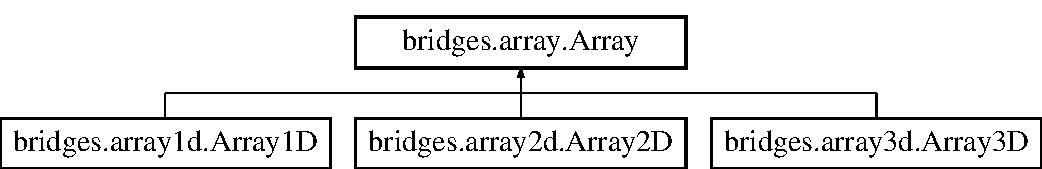
\includegraphics[height=2.000000cm]{classbridges_1_1array_1_1_array}
\end{center}
\end{figure}


\doxysubsection{Detailed Description}
This class can be used to create arrays of type Element$<$\+E$>$. 

\begin{DoxyAuthor}{Author}
Matthew Mc\+Quaigue
\end{DoxyAuthor}
\begin{DoxyDate}{Date}
10/8/16, 6/09/19
\end{DoxyDate}
This class can be used to create arrays of type Element$<$\+E$>$ where E is a generic object representing application specific data.

Arrays are internally represented as 1D arrays; currently 1D, 2D and 3D arrays are supported.

Example Tutorial at\+: \href{https://bridgesuncc.github.io/tutorials/Array.html}{\texttt{ https\+://bridgesuncc.\+github.\+io/tutorials/\+Array.\+html}} (1D, 2D, and 3D \mbox{\hyperlink{classbridges_1_1array_1_1_array}{Array}}) \doxysubsection*{Public Member Functions}
\begin{DoxyCompactItemize}
\item 
def \mbox{\hyperlink{classbridges_1_1array_1_1_array_a84c1237ed71850f141cd0cac5a8f77c3}{\+\_\+\+\_\+init\+\_\+\+\_\+}} (self, $\ast$$\ast$kwargs)
\begin{DoxyCompactList}\small\item\em \mbox{\hyperlink{classbridges_1_1array_1_1_array}{Array}} constructor. \end{DoxyCompactList}\item 
int \mbox{\hyperlink{classbridges_1_1array_1_1_array_a4d7ea01781326e1b07a297f54ddcba2d}{num\+\_\+dims}} (self)
\begin{DoxyCompactList}\small\item\em Getter for representing the number of dimensions in the array. \end{DoxyCompactList}\item 
None \mbox{\hyperlink{classbridges_1_1array_1_1_array_afea12a8b38ac62d46413e557c3c1d89d}{num\+\_\+dims}} (self, int value)
\begin{DoxyCompactList}\small\item\em Setter function for the number of dimensions for the array. \end{DoxyCompactList}\item 
int \mbox{\hyperlink{classbridges_1_1array_1_1_array_a479be9c2ec7aace6db3bec8b48a53ac7}{size}} (self)
\begin{DoxyCompactList}\small\item\em Getter for representing the size of array. \end{DoxyCompactList}\item 
None \mbox{\hyperlink{classbridges_1_1array_1_1_array_a50f6b3cf7794221428038cc84f868e25}{size}} (self, int sz)
\begin{DoxyCompactList}\small\item\em Setter for representing the size of the array. \end{DoxyCompactList}\item 
None \mbox{\hyperlink{classbridges_1_1array_1_1_array_aa503ee9a06a60ddf8acb9e5dc49c820a}{set\+\_\+size}} (self, int nd, list dim)
\begin{DoxyCompactList}\small\item\em Set the size of each dimensions; also allocates array space. \end{DoxyCompactList}\item 
str \mbox{\hyperlink{classbridges_1_1array_1_1_array_aa52e4e7984fa0cc6ed1f160d25dfe14e}{get\+\_\+data\+\_\+structure\+\_\+type}} (self)
\begin{DoxyCompactList}\small\item\em Gets the data structure type. \end{DoxyCompactList}\item 
list \mbox{\hyperlink{classbridges_1_1array_1_1_array_a522509608957badbb17197b0bb7d11e6}{get\+\_\+dimensions}} (self)
\begin{DoxyCompactList}\small\item\em Get the size of each dimensions. \end{DoxyCompactList}\item 
def \mbox{\hyperlink{classbridges_1_1array_1_1_array_a2951a024fefc11202bc8036b2314bb42}{get\+\_\+element}} (self, $\ast$args, $\ast$$\ast$kwargs)
\begin{DoxyCompactList}\small\item\em Getter function for an element in the array at given position. \end{DoxyCompactList}\item 
def \mbox{\hyperlink{classbridges_1_1array_1_1_array_ab43ea53de915dec3a57c32918979300b}{set\+\_\+element}} (self, $\ast$args, $\ast$$\ast$kwargs)
\begin{DoxyCompactList}\small\item\em Setter function for an element in the array at given position. \end{DoxyCompactList}\item 
def \mbox{\hyperlink{classbridges_1_1array_1_1_array_ad97d5a2cb4bffa4a6bcdb15a3ece0974}{\+\_\+\+\_\+getitem\+\_\+\+\_\+}} (self, item)
\item 
def \mbox{\hyperlink{classbridges_1_1array_1_1_array_a97fd57b09a0b8ae221ecaa50c1c483b1}{\+\_\+\+\_\+setitem\+\_\+\+\_\+}} (self, key, value)
\item 
dict \mbox{\hyperlink{classbridges_1_1array_1_1_array_aaec9bd4d74389f4de5a47f3485a47ce0}{get\+\_\+data\+\_\+structure\+\_\+representation}} (self)
\begin{DoxyCompactList}\small\item\em Generating the JSON string for a bridges array object. \end{DoxyCompactList}\end{DoxyCompactItemize}
\doxysubsection*{Public Attributes}
\begin{DoxyCompactItemize}
\item 
\mbox{\hyperlink{classbridges_1_1array_1_1_array_a2c28c3658312289dc2ae78f4099d4c76}{num\+\_\+dims}}
\item 
\mbox{\hyperlink{classbridges_1_1array_1_1_array_aeac1b1639d0284500f354d41b40c38f7}{size}}
\end{DoxyCompactItemize}
\doxysubsection*{Static Public Attributes}
\begin{DoxyCompactItemize}
\item 
list \mbox{\hyperlink{classbridges_1_1array_1_1_array_a69f2c673a6077e203b3e916dd73cd243}{dims}} = \mbox{[}1,1,1\mbox{]}
\end{DoxyCompactItemize}


\doxysubsection{Constructor \& Destructor Documentation}
\mbox{\Hypertarget{classbridges_1_1array_1_1_array_a84c1237ed71850f141cd0cac5a8f77c3}\label{classbridges_1_1array_1_1_array_a84c1237ed71850f141cd0cac5a8f77c3}} 
\index{bridges.array.Array@{bridges.array.Array}!\_\_init\_\_@{\_\_init\_\_}}
\index{\_\_init\_\_@{\_\_init\_\_}!bridges.array.Array@{bridges.array.Array}}
\doxysubsubsection{\texorpdfstring{\_\_init\_\_()}{\_\_init\_\_()}}
{\footnotesize\ttfamily def bridges.\+array.\+Array.\+\_\+\+\_\+init\+\_\+\+\_\+ (\begin{DoxyParamCaption}\item[{}]{self,  }\item[{$\ast$$\ast$}]{kwargs }\end{DoxyParamCaption})}



\mbox{\hyperlink{classbridges_1_1array_1_1_array}{Array}} constructor. 


\begin{DoxyParams}{Parameters}
{\em dims} & size of each dimension (array) \\
\hline
{\em num\+\_\+dims} & The dimensions of the array (1-\/3). Defaults to 1 dimension (int) \\
\hline
\end{DoxyParams}
\begin{DoxyReturn}{Returns}


None 
\end{DoxyReturn}


Reimplemented in \mbox{\hyperlink{classbridges_1_1array3d_1_1_array3_d_a24ea126f1007b53eaf420e32f086cac3}{bridges.\+array3d.\+Array3D}}.



\doxysubsection{Member Function Documentation}
\mbox{\Hypertarget{classbridges_1_1array_1_1_array_ad97d5a2cb4bffa4a6bcdb15a3ece0974}\label{classbridges_1_1array_1_1_array_ad97d5a2cb4bffa4a6bcdb15a3ece0974}} 
\index{bridges.array.Array@{bridges.array.Array}!\_\_getitem\_\_@{\_\_getitem\_\_}}
\index{\_\_getitem\_\_@{\_\_getitem\_\_}!bridges.array.Array@{bridges.array.Array}}
\doxysubsubsection{\texorpdfstring{\_\_getitem\_\_()}{\_\_getitem\_\_()}}
{\footnotesize\ttfamily def bridges.\+array.\+Array.\+\_\+\+\_\+getitem\+\_\+\+\_\+ (\begin{DoxyParamCaption}\item[{}]{self,  }\item[{}]{item }\end{DoxyParamCaption})}

\mbox{\Hypertarget{classbridges_1_1array_1_1_array_a97fd57b09a0b8ae221ecaa50c1c483b1}\label{classbridges_1_1array_1_1_array_a97fd57b09a0b8ae221ecaa50c1c483b1}} 
\index{bridges.array.Array@{bridges.array.Array}!\_\_setitem\_\_@{\_\_setitem\_\_}}
\index{\_\_setitem\_\_@{\_\_setitem\_\_}!bridges.array.Array@{bridges.array.Array}}
\doxysubsubsection{\texorpdfstring{\_\_setitem\_\_()}{\_\_setitem\_\_()}}
{\footnotesize\ttfamily def bridges.\+array.\+Array.\+\_\+\+\_\+setitem\+\_\+\+\_\+ (\begin{DoxyParamCaption}\item[{}]{self,  }\item[{}]{key,  }\item[{}]{value }\end{DoxyParamCaption})}

\mbox{\Hypertarget{classbridges_1_1array_1_1_array_aaec9bd4d74389f4de5a47f3485a47ce0}\label{classbridges_1_1array_1_1_array_aaec9bd4d74389f4de5a47f3485a47ce0}} 
\index{bridges.array.Array@{bridges.array.Array}!get\_data\_structure\_representation@{get\_data\_structure\_representation}}
\index{get\_data\_structure\_representation@{get\_data\_structure\_representation}!bridges.array.Array@{bridges.array.Array}}
\doxysubsubsection{\texorpdfstring{get\_data\_structure\_representation()}{get\_data\_structure\_representation()}}
{\footnotesize\ttfamily  dict bridges.\+array.\+Array.\+get\+\_\+data\+\_\+structure\+\_\+representation (\begin{DoxyParamCaption}\item[{}]{self }\end{DoxyParamCaption})}



Generating the JSON string for a bridges array object. 

\begin{DoxyReturn}{Returns}


dict the dict that will represent the json when dumped 
\end{DoxyReturn}
\mbox{\Hypertarget{classbridges_1_1array_1_1_array_aa52e4e7984fa0cc6ed1f160d25dfe14e}\label{classbridges_1_1array_1_1_array_aa52e4e7984fa0cc6ed1f160d25dfe14e}} 
\index{bridges.array.Array@{bridges.array.Array}!get\_data\_structure\_type@{get\_data\_structure\_type}}
\index{get\_data\_structure\_type@{get\_data\_structure\_type}!bridges.array.Array@{bridges.array.Array}}
\doxysubsubsection{\texorpdfstring{get\_data\_structure\_type()}{get\_data\_structure\_type()}}
{\footnotesize\ttfamily  str bridges.\+array.\+Array.\+get\+\_\+data\+\_\+structure\+\_\+type (\begin{DoxyParamCaption}\item[{}]{self }\end{DoxyParamCaption})}



Gets the data structure type. 


\begin{DoxyExceptions}{Exceptions}
{\em Value\+Error} & if number of dimensions is $<$ 1 or $>$ 3 \\
\hline
\end{DoxyExceptions}
\begin{DoxyReturn}{Returns}


str type of data structure 
\end{DoxyReturn}
\mbox{\Hypertarget{classbridges_1_1array_1_1_array_a522509608957badbb17197b0bb7d11e6}\label{classbridges_1_1array_1_1_array_a522509608957badbb17197b0bb7d11e6}} 
\index{bridges.array.Array@{bridges.array.Array}!get\_dimensions@{get\_dimensions}}
\index{get\_dimensions@{get\_dimensions}!bridges.array.Array@{bridges.array.Array}}
\doxysubsubsection{\texorpdfstring{get\_dimensions()}{get\_dimensions()}}
{\footnotesize\ttfamily  list bridges.\+array.\+Array.\+get\+\_\+dimensions (\begin{DoxyParamCaption}\item[{}]{self }\end{DoxyParamCaption})}



Get the size of each dimensions. 

\begin{DoxyReturn}{Returns}


list size of each dimension 
\end{DoxyReturn}
\mbox{\Hypertarget{classbridges_1_1array_1_1_array_a2951a024fefc11202bc8036b2314bb42}\label{classbridges_1_1array_1_1_array_a2951a024fefc11202bc8036b2314bb42}} 
\index{bridges.array.Array@{bridges.array.Array}!get\_element@{get\_element}}
\index{get\_element@{get\_element}!bridges.array.Array@{bridges.array.Array}}
\doxysubsubsection{\texorpdfstring{get\_element()}{get\_element()}}
{\footnotesize\ttfamily def bridges.\+array.\+Array.\+get\+\_\+element (\begin{DoxyParamCaption}\item[{}]{self,  }\item[{$\ast$}]{args,  }\item[{$\ast$$\ast$}]{kwargs }\end{DoxyParamCaption})}



Getter function for an element in the array at given position. 

\begin{DoxyVerb}       (int) x,y,z,: indices

       (int) index: the index of array to get in array
       (int) x: column index into array
       (int) y: row index into array
       (int) z: slice index into array
\end{DoxyVerb}
 \begin{DoxyReturn}{Returns}


Element the element at position given 
\end{DoxyReturn}
\mbox{\Hypertarget{classbridges_1_1array_1_1_array_a4d7ea01781326e1b07a297f54ddcba2d}\label{classbridges_1_1array_1_1_array_a4d7ea01781326e1b07a297f54ddcba2d}} 
\index{bridges.array.Array@{bridges.array.Array}!num\_dims@{num\_dims}}
\index{num\_dims@{num\_dims}!bridges.array.Array@{bridges.array.Array}}
\doxysubsubsection{\texorpdfstring{num\_dims()}{num\_dims()}\hspace{0.1cm}{\footnotesize\ttfamily [1/2]}}
{\footnotesize\ttfamily  int bridges.\+array.\+Array.\+num\+\_\+dims (\begin{DoxyParamCaption}\item[{}]{self }\end{DoxyParamCaption})}



Getter for representing the number of dimensions in the array. 

\begin{DoxyReturn}{Returns}


int number of dimensions 
\end{DoxyReturn}
\mbox{\Hypertarget{classbridges_1_1array_1_1_array_afea12a8b38ac62d46413e557c3c1d89d}\label{classbridges_1_1array_1_1_array_afea12a8b38ac62d46413e557c3c1d89d}} 
\index{bridges.array.Array@{bridges.array.Array}!num\_dims@{num\_dims}}
\index{num\_dims@{num\_dims}!bridges.array.Array@{bridges.array.Array}}
\doxysubsubsection{\texorpdfstring{num\_dims()}{num\_dims()}\hspace{0.1cm}{\footnotesize\ttfamily [2/2]}}
{\footnotesize\ttfamily  None bridges.\+array.\+Array.\+num\+\_\+dims (\begin{DoxyParamCaption}\item[{}]{self,  }\item[{int}]{value }\end{DoxyParamCaption})}



Setter function for the number of dimensions for the array. 


\begin{DoxyParams}{Parameters}
{\em value} & An integer for the number of dimensions (Between 1 and 3 inclusive) \\
\hline
\end{DoxyParams}
\begin{DoxyReturn}{Returns}


None
\end{DoxyReturn}

\begin{DoxyExceptions}{Exceptions}
{\em Value\+Error} & if dimension passed in is $<$ 1 or $>$ 3 \\
\hline
\end{DoxyExceptions}
\mbox{\Hypertarget{classbridges_1_1array_1_1_array_ab43ea53de915dec3a57c32918979300b}\label{classbridges_1_1array_1_1_array_ab43ea53de915dec3a57c32918979300b}} 
\index{bridges.array.Array@{bridges.array.Array}!set\_element@{set\_element}}
\index{set\_element@{set\_element}!bridges.array.Array@{bridges.array.Array}}
\doxysubsubsection{\texorpdfstring{set\_element()}{set\_element()}}
{\footnotesize\ttfamily def bridges.\+array.\+Array.\+set\+\_\+element (\begin{DoxyParamCaption}\item[{}]{self,  }\item[{$\ast$}]{args,  }\item[{$\ast$$\ast$}]{kwargs }\end{DoxyParamCaption})}



Setter function for an element in the array at given position. 

\begin{DoxyVerb}       (int) x,y,z: indices
       (Element) el: element object to be assigned to index, always last position arg if using unnamed args

       (Element) el: element object to be assigned to index
       (int) index: the index of array to get in array
       (int) x: column index into array
       (int) y: row index into array
       (int) z: slice index into array
\end{DoxyVerb}
 \begin{DoxyReturn}{Returns}


None 
\end{DoxyReturn}
\mbox{\Hypertarget{classbridges_1_1array_1_1_array_aa503ee9a06a60ddf8acb9e5dc49c820a}\label{classbridges_1_1array_1_1_array_aa503ee9a06a60ddf8acb9e5dc49c820a}} 
\index{bridges.array.Array@{bridges.array.Array}!set\_size@{set\_size}}
\index{set\_size@{set\_size}!bridges.array.Array@{bridges.array.Array}}
\doxysubsubsection{\texorpdfstring{set\_size()}{set\_size()}}
{\footnotesize\ttfamily  None bridges.\+array.\+Array.\+set\+\_\+size (\begin{DoxyParamCaption}\item[{}]{self,  }\item[{int}]{nd,  }\item[{list}]{dim }\end{DoxyParamCaption})}



Set the size of each dimensions; also allocates array space. 

\begin{DoxyVerb}       (int) nd: number of dimensions
       (list) dim: size of each dimension
\end{DoxyVerb}
 \begin{DoxyReturn}{Returns}


None 
\end{DoxyReturn}
\mbox{\Hypertarget{classbridges_1_1array_1_1_array_a479be9c2ec7aace6db3bec8b48a53ac7}\label{classbridges_1_1array_1_1_array_a479be9c2ec7aace6db3bec8b48a53ac7}} 
\index{bridges.array.Array@{bridges.array.Array}!size@{size}}
\index{size@{size}!bridges.array.Array@{bridges.array.Array}}
\doxysubsubsection{\texorpdfstring{size()}{size()}\hspace{0.1cm}{\footnotesize\ttfamily [1/2]}}
{\footnotesize\ttfamily  int bridges.\+array.\+Array.\+size (\begin{DoxyParamCaption}\item[{}]{self }\end{DoxyParamCaption})}



Getter for representing the size of array. 

\begin{DoxyReturn}{Returns}


int the size 
\end{DoxyReturn}
\mbox{\Hypertarget{classbridges_1_1array_1_1_array_a50f6b3cf7794221428038cc84f868e25}\label{classbridges_1_1array_1_1_array_a50f6b3cf7794221428038cc84f868e25}} 
\index{bridges.array.Array@{bridges.array.Array}!size@{size}}
\index{size@{size}!bridges.array.Array@{bridges.array.Array}}
\doxysubsubsection{\texorpdfstring{size()}{size()}\hspace{0.1cm}{\footnotesize\ttfamily [2/2]}}
{\footnotesize\ttfamily  None bridges.\+array.\+Array.\+size (\begin{DoxyParamCaption}\item[{}]{self,  }\item[{int}]{sz }\end{DoxyParamCaption})}



Setter for representing the size of the array. 

\begin{DoxyVerb}       (int) sz: The size to be set for array
\end{DoxyVerb}
 \begin{DoxyReturn}{Returns}


None 
\end{DoxyReturn}


\doxysubsection{Member Data Documentation}
\mbox{\Hypertarget{classbridges_1_1array_1_1_array_a69f2c673a6077e203b3e916dd73cd243}\label{classbridges_1_1array_1_1_array_a69f2c673a6077e203b3e916dd73cd243}} 
\index{bridges.array.Array@{bridges.array.Array}!dims@{dims}}
\index{dims@{dims}!bridges.array.Array@{bridges.array.Array}}
\doxysubsubsection{\texorpdfstring{dims}{dims}}
{\footnotesize\ttfamily list bridges.\+array.\+Array.\+dims = \mbox{[}1,1,1\mbox{]}\hspace{0.3cm}{\ttfamily [static]}}

\mbox{\Hypertarget{classbridges_1_1array_1_1_array_a2c28c3658312289dc2ae78f4099d4c76}\label{classbridges_1_1array_1_1_array_a2c28c3658312289dc2ae78f4099d4c76}} 
\index{bridges.array.Array@{bridges.array.Array}!num\_dims@{num\_dims}}
\index{num\_dims@{num\_dims}!bridges.array.Array@{bridges.array.Array}}
\doxysubsubsection{\texorpdfstring{num\_dims}{num\_dims}}
{\footnotesize\ttfamily bridges.\+array.\+Array.\+num\+\_\+dims}

\mbox{\Hypertarget{classbridges_1_1array_1_1_array_aeac1b1639d0284500f354d41b40c38f7}\label{classbridges_1_1array_1_1_array_aeac1b1639d0284500f354d41b40c38f7}} 
\index{bridges.array.Array@{bridges.array.Array}!size@{size}}
\index{size@{size}!bridges.array.Array@{bridges.array.Array}}
\doxysubsubsection{\texorpdfstring{size}{size}}
{\footnotesize\ttfamily bridges.\+array.\+Array.\+size}



The documentation for this class was generated from the following file\+:\begin{DoxyCompactItemize}
\item 
/\+Users/kalpathi/gr/bridges/client/python/bridges/\mbox{\hyperlink{array_8py}{array.\+py}}\end{DoxyCompactItemize}

\hypertarget{classbridges_1_1avl__tree__element_1_1_a_v_l_tree_element}{}\section{bridges.\+avl\+\_\+tree\+\_\+element.\+A\+V\+L\+Tree\+Element Class Reference}
\label{classbridges_1_1avl__tree__element_1_1_a_v_l_tree_element}\index{bridges.avl\_tree\_element.AVLTreeElement@{bridges.avl\_tree\_element.AVLTreeElement}}
Inheritance diagram for bridges.\+avl\+\_\+tree\+\_\+element.\+A\+V\+L\+Tree\+Element\+:\begin{figure}[H]
\begin{center}
\leavevmode
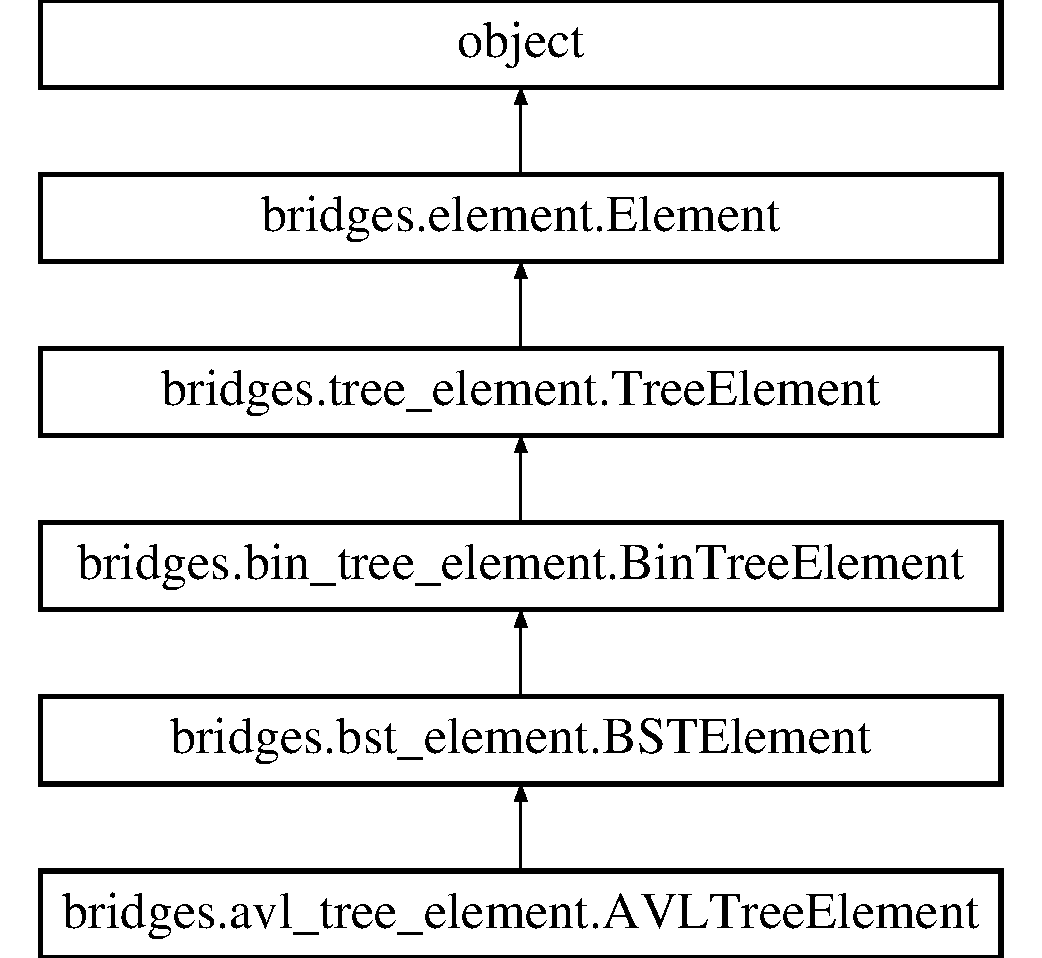
\includegraphics[height=5.000000cm]{classbridges_1_1avl__tree__element_1_1_a_v_l_tree_element}
\end{center}
\end{figure}


\subsection{Detailed Description}
This class extends the B\+S\+T\+Element class by adding a height and balance factor fields that are useful in A\+VL trees. 

A\+VL tree elements include a \textquotesingle{}height\textquotesingle{} and a \textquotesingle{}bal\+Factor\textquotesingle{} value, representing the height and balance factor of the A\+VL tree at that node, respectively. This is useful in representing A\+VL trees.

A\+V\+L\+Tree elements contain a visualizer (Element\+Visualizer) object for setting visual attributes (color, shape, opacity, size), necessary for displaying them in a web browser.

A\+V\+L\+Tree elements also have a Link\+Visualizer object, that is used when they are linked to another element, appropriate for setting link attributes, for instance, between the current element and its left or right child

\begin{DoxyAuthor}{Author}
Kalpathi Subramanian, Mihai Mehedint, Matthew Mc\+Quaigue
\end{DoxyAuthor}
\begin{DoxyDate}{Date}
6/22/16, 1/7/17, 5/17/17, 6/09/19
\end{DoxyDate}
Example tutorial using \mbox{\hyperlink{classbridges_1_1avl__tree__element_1_1_a_v_l_tree_element}{A\+V\+L\+Tree\+Element}} at\+: \href{http://bridgesuncc.github.io/tutorials/AVL.html}{\texttt{ http\+://bridgesuncc.\+github.\+io/tutorials/\+A\+V\+L.\+html}} \subsection*{Public Member Functions}
\begin{DoxyCompactItemize}
\item 
None \mbox{\hyperlink{classbridges_1_1avl__tree__element_1_1_a_v_l_tree_element_a5c07b41b6a37b9392b3ecea517d2d0ea}{\+\_\+\+\_\+init\+\_\+\+\_\+}} (self, $\ast$args, $\ast$$\ast$kwargs)
\begin{DoxyCompactList}\small\item\em A\+VL Tree constructor. \end{DoxyCompactList}\item 
str \mbox{\hyperlink{classbridges_1_1avl__tree__element_1_1_a_v_l_tree_element_a811dd4cebd36fda6531f6cbeb873c0e5}{get\+\_\+data\+\_\+structure\+\_\+type}} (self)
\begin{DoxyCompactList}\small\item\em Get the data structure type. \end{DoxyCompactList}\item 
str \mbox{\hyperlink{classbridges_1_1avl__tree__element_1_1_a_v_l_tree_element_ac830bbf88d156574fd23a8b1eaa6bc69}{key}} (self)
\begin{DoxyCompactList}\small\item\em Getter for the search keys. \end{DoxyCompactList}\item 
int \mbox{\hyperlink{classbridges_1_1avl__tree__element_1_1_a_v_l_tree_element_af32b7f1985abf0f6c0573cc23fef63b6}{height}} (self)
\begin{DoxyCompactList}\small\item\em Getter for height of the avl tree at this node. \end{DoxyCompactList}\item 
None \mbox{\hyperlink{classbridges_1_1avl__tree__element_1_1_a_v_l_tree_element_acc82ab37af6763d759493fd708218702}{height}} (self, int \mbox{\hyperlink{classbridges_1_1element_1_1_element_ad18e8738e025d7af322144aecbec1629}{value}})
\begin{DoxyCompactList}\small\item\em Setter function for the height of the avl tree. \end{DoxyCompactList}\item 
int \mbox{\hyperlink{classbridges_1_1avl__tree__element_1_1_a_v_l_tree_element_a55d0ce96bb49325807232aa084876505}{balance\+\_\+factor}} (self)
\begin{DoxyCompactList}\small\item\em Getter for the balance factor of the tree at this node. \end{DoxyCompactList}\item 
None \mbox{\hyperlink{classbridges_1_1avl__tree__element_1_1_a_v_l_tree_element_aaf931b718c678cfc919e2267d1efa412}{balance\+\_\+factor}} (self, int \mbox{\hyperlink{classbridges_1_1element_1_1_element_ad18e8738e025d7af322144aecbec1629}{value}})
\begin{DoxyCompactList}\small\item\em Setter for the balance factor of the tree at this node. \end{DoxyCompactList}\item 
def \mbox{\hyperlink{classbridges_1_1avl__tree__element_1_1_a_v_l_tree_element_a717696b26736f5c9585fefc7c5ab88f1}{left}} (self)
\begin{DoxyCompactList}\small\item\em Getter for the left child of the avl tree. \end{DoxyCompactList}\item 
None \mbox{\hyperlink{classbridges_1_1avl__tree__element_1_1_a_v_l_tree_element_a5ee29c8a42e07019a77ecd7a2534f8be}{left}} (self, val)
\begin{DoxyCompactList}\small\item\em Setter for the left child of the avl tree. \end{DoxyCompactList}\item 
def \mbox{\hyperlink{classbridges_1_1avl__tree__element_1_1_a_v_l_tree_element_aaab3b79617e7e503b1a7c28069d1eb15}{right}} (self)
\begin{DoxyCompactList}\small\item\em Getter for the right child of the avl tree. \end{DoxyCompactList}\item 
None \mbox{\hyperlink{classbridges_1_1avl__tree__element_1_1_a_v_l_tree_element_a5aa36d46b0c6ac791893823500c77a08}{right}} (self, val)
\begin{DoxyCompactList}\small\item\em Setter for the right child of the avl tree. \end{DoxyCompactList}\item 
dict \mbox{\hyperlink{classbridges_1_1avl__tree__element_1_1_a_v_l_tree_element_abf8842cb462f1e31f0889d67fb0d70d4}{get\+\_\+element\+\_\+representation}} (self)
\begin{DoxyCompactList}\small\item\em Augment the element with the \char`\"{}height\char`\"{} and \char`\"{}balance factor\char`\"{} fields. \end{DoxyCompactList}\end{DoxyCompactItemize}
\subsection*{Additional Inherited Members}


\subsection{Constructor \& Destructor Documentation}
\mbox{\Hypertarget{classbridges_1_1avl__tree__element_1_1_a_v_l_tree_element_a5c07b41b6a37b9392b3ecea517d2d0ea}\label{classbridges_1_1avl__tree__element_1_1_a_v_l_tree_element_a5c07b41b6a37b9392b3ecea517d2d0ea}} 
\index{bridges.avl\_tree\_element.AVLTreeElement@{bridges.avl\_tree\_element.AVLTreeElement}!\_\_init\_\_@{\_\_init\_\_}}
\index{\_\_init\_\_@{\_\_init\_\_}!bridges.avl\_tree\_element.AVLTreeElement@{bridges.avl\_tree\_element.AVLTreeElement}}
\subsubsection{\texorpdfstring{\_\_init\_\_()}{\_\_init\_\_()}}
{\footnotesize\ttfamily  None bridges.\+avl\+\_\+tree\+\_\+element.\+A\+V\+L\+Tree\+Element.\+\_\+\+\_\+init\+\_\+\+\_\+ (\begin{DoxyParamCaption}\item[{}]{self,  }\item[{$\ast$}]{args,  }\item[{$\ast$$\ast$}]{kwargs }\end{DoxyParamCaption})}



A\+VL Tree constructor. 


\begin{DoxyParams}{Parameters}
{\em key} & \\
\hline
{\em element} & \\
\hline
{\em key} & the search key \\
\hline
{\em e} & the the specific object that the element is holding \\
\hline
\end{DoxyParams}
\begin{DoxyReturn}{Returns}


None 
\end{DoxyReturn}


\subsection{Member Function Documentation}
\mbox{\Hypertarget{classbridges_1_1avl__tree__element_1_1_a_v_l_tree_element_a55d0ce96bb49325807232aa084876505}\label{classbridges_1_1avl__tree__element_1_1_a_v_l_tree_element_a55d0ce96bb49325807232aa084876505}} 
\index{bridges.avl\_tree\_element.AVLTreeElement@{bridges.avl\_tree\_element.AVLTreeElement}!balance\_factor@{balance\_factor}}
\index{balance\_factor@{balance\_factor}!bridges.avl\_tree\_element.AVLTreeElement@{bridges.avl\_tree\_element.AVLTreeElement}}
\subsubsection{\texorpdfstring{balance\_factor()}{balance\_factor()}\hspace{0.1cm}{\footnotesize\ttfamily [1/2]}}
{\footnotesize\ttfamily  int bridges.\+avl\+\_\+tree\+\_\+element.\+A\+V\+L\+Tree\+Element.\+balance\+\_\+factor (\begin{DoxyParamCaption}\item[{}]{self }\end{DoxyParamCaption})}



Getter for the balance factor of the tree at this node. 

\begin{DoxyReturn}{Returns}


int representing the balance factor 
\end{DoxyReturn}
\mbox{\Hypertarget{classbridges_1_1avl__tree__element_1_1_a_v_l_tree_element_aaf931b718c678cfc919e2267d1efa412}\label{classbridges_1_1avl__tree__element_1_1_a_v_l_tree_element_aaf931b718c678cfc919e2267d1efa412}} 
\index{bridges.avl\_tree\_element.AVLTreeElement@{bridges.avl\_tree\_element.AVLTreeElement}!balance\_factor@{balance\_factor}}
\index{balance\_factor@{balance\_factor}!bridges.avl\_tree\_element.AVLTreeElement@{bridges.avl\_tree\_element.AVLTreeElement}}
\subsubsection{\texorpdfstring{balance\_factor()}{balance\_factor()}\hspace{0.1cm}{\footnotesize\ttfamily [2/2]}}
{\footnotesize\ttfamily  None bridges.\+avl\+\_\+tree\+\_\+element.\+A\+V\+L\+Tree\+Element.\+balance\+\_\+factor (\begin{DoxyParamCaption}\item[{}]{self,  }\item[{int}]{value }\end{DoxyParamCaption})}



Setter for the balance factor of the tree at this node. 

\begin{DoxyVerb}       (int) value: An integer for the balance factor at this node
\end{DoxyVerb}
 \begin{DoxyReturn}{Returns}


None 
\end{DoxyReturn}
\mbox{\Hypertarget{classbridges_1_1avl__tree__element_1_1_a_v_l_tree_element_a811dd4cebd36fda6531f6cbeb873c0e5}\label{classbridges_1_1avl__tree__element_1_1_a_v_l_tree_element_a811dd4cebd36fda6531f6cbeb873c0e5}} 
\index{bridges.avl\_tree\_element.AVLTreeElement@{bridges.avl\_tree\_element.AVLTreeElement}!get\_data\_structure\_type@{get\_data\_structure\_type}}
\index{get\_data\_structure\_type@{get\_data\_structure\_type}!bridges.avl\_tree\_element.AVLTreeElement@{bridges.avl\_tree\_element.AVLTreeElement}}
\subsubsection{\texorpdfstring{get\_data\_structure\_type()}{get\_data\_structure\_type()}}
{\footnotesize\ttfamily  str bridges.\+avl\+\_\+tree\+\_\+element.\+A\+V\+L\+Tree\+Element.\+get\+\_\+data\+\_\+structure\+\_\+type (\begin{DoxyParamCaption}\item[{}]{self }\end{DoxyParamCaption})}



Get the data structure type. 

\begin{DoxyReturn}{Returns}


str the type of data structure 
\end{DoxyReturn}


Reimplemented from \mbox{\hyperlink{classbridges_1_1bst__element_1_1_b_s_t_element_a8e655e06ba0f77b7e2681b6d291f39de}{bridges.\+bst\+\_\+element.\+B\+S\+T\+Element}}.

\mbox{\Hypertarget{classbridges_1_1avl__tree__element_1_1_a_v_l_tree_element_abf8842cb462f1e31f0889d67fb0d70d4}\label{classbridges_1_1avl__tree__element_1_1_a_v_l_tree_element_abf8842cb462f1e31f0889d67fb0d70d4}} 
\index{bridges.avl\_tree\_element.AVLTreeElement@{bridges.avl\_tree\_element.AVLTreeElement}!get\_element\_representation@{get\_element\_representation}}
\index{get\_element\_representation@{get\_element\_representation}!bridges.avl\_tree\_element.AVLTreeElement@{bridges.avl\_tree\_element.AVLTreeElement}}
\subsubsection{\texorpdfstring{get\_element\_representation()}{get\_element\_representation()}}
{\footnotesize\ttfamily  dict bridges.\+avl\+\_\+tree\+\_\+element.\+A\+V\+L\+Tree\+Element.\+get\+\_\+element\+\_\+representation (\begin{DoxyParamCaption}\item[{}]{self }\end{DoxyParamCaption})}



Augment the element with the \char`\"{}height\char`\"{} and \char`\"{}balance factor\char`\"{} fields. 

\begin{DoxyReturn}{Returns}


dict representing the json of this element 
\end{DoxyReturn}


Reimplemented from \mbox{\hyperlink{classbridges_1_1bst__element_1_1_b_s_t_element_a9d038f191a7cf06e75910463a3aa3b80}{bridges.\+bst\+\_\+element.\+B\+S\+T\+Element}}.

\mbox{\Hypertarget{classbridges_1_1avl__tree__element_1_1_a_v_l_tree_element_af32b7f1985abf0f6c0573cc23fef63b6}\label{classbridges_1_1avl__tree__element_1_1_a_v_l_tree_element_af32b7f1985abf0f6c0573cc23fef63b6}} 
\index{bridges.avl\_tree\_element.AVLTreeElement@{bridges.avl\_tree\_element.AVLTreeElement}!height@{height}}
\index{height@{height}!bridges.avl\_tree\_element.AVLTreeElement@{bridges.avl\_tree\_element.AVLTreeElement}}
\subsubsection{\texorpdfstring{height()}{height()}\hspace{0.1cm}{\footnotesize\ttfamily [1/2]}}
{\footnotesize\ttfamily  int bridges.\+avl\+\_\+tree\+\_\+element.\+A\+V\+L\+Tree\+Element.\+height (\begin{DoxyParamCaption}\item[{}]{self }\end{DoxyParamCaption})}



Getter for height of the avl tree at this node. 

\begin{DoxyReturn}{Returns}


int the height of the tree 
\end{DoxyReturn}
\mbox{\Hypertarget{classbridges_1_1avl__tree__element_1_1_a_v_l_tree_element_acc82ab37af6763d759493fd708218702}\label{classbridges_1_1avl__tree__element_1_1_a_v_l_tree_element_acc82ab37af6763d759493fd708218702}} 
\index{bridges.avl\_tree\_element.AVLTreeElement@{bridges.avl\_tree\_element.AVLTreeElement}!height@{height}}
\index{height@{height}!bridges.avl\_tree\_element.AVLTreeElement@{bridges.avl\_tree\_element.AVLTreeElement}}
\subsubsection{\texorpdfstring{height()}{height()}\hspace{0.1cm}{\footnotesize\ttfamily [2/2]}}
{\footnotesize\ttfamily  None bridges.\+avl\+\_\+tree\+\_\+element.\+A\+V\+L\+Tree\+Element.\+height (\begin{DoxyParamCaption}\item[{}]{self,  }\item[{int}]{value }\end{DoxyParamCaption})}



Setter function for the height of the avl tree. 

\begin{DoxyVerb}       (int) value: An integer for the height at this node
\end{DoxyVerb}
 \begin{DoxyReturn}{Returns}


None 
\end{DoxyReturn}
\mbox{\Hypertarget{classbridges_1_1avl__tree__element_1_1_a_v_l_tree_element_ac830bbf88d156574fd23a8b1eaa6bc69}\label{classbridges_1_1avl__tree__element_1_1_a_v_l_tree_element_ac830bbf88d156574fd23a8b1eaa6bc69}} 
\index{bridges.avl\_tree\_element.AVLTreeElement@{bridges.avl\_tree\_element.AVLTreeElement}!key@{key}}
\index{key@{key}!bridges.avl\_tree\_element.AVLTreeElement@{bridges.avl\_tree\_element.AVLTreeElement}}
\subsubsection{\texorpdfstring{key()}{key()}}
{\footnotesize\ttfamily  str bridges.\+avl\+\_\+tree\+\_\+element.\+A\+V\+L\+Tree\+Element.\+key (\begin{DoxyParamCaption}\item[{}]{self }\end{DoxyParamCaption})}



Getter for the search keys. 

\begin{DoxyReturn}{Returns}


str represeting the key 
\end{DoxyReturn}


Reimplemented from \mbox{\hyperlink{classbridges_1_1bst__element_1_1_b_s_t_element_ae911a11782ad4623b21781c5eeeb7d39}{bridges.\+bst\+\_\+element.\+B\+S\+T\+Element}}.

\mbox{\Hypertarget{classbridges_1_1avl__tree__element_1_1_a_v_l_tree_element_a717696b26736f5c9585fefc7c5ab88f1}\label{classbridges_1_1avl__tree__element_1_1_a_v_l_tree_element_a717696b26736f5c9585fefc7c5ab88f1}} 
\index{bridges.avl\_tree\_element.AVLTreeElement@{bridges.avl\_tree\_element.AVLTreeElement}!left@{left}}
\index{left@{left}!bridges.avl\_tree\_element.AVLTreeElement@{bridges.avl\_tree\_element.AVLTreeElement}}
\subsubsection{\texorpdfstring{left()}{left()}\hspace{0.1cm}{\footnotesize\ttfamily [1/2]}}
{\footnotesize\ttfamily def bridges.\+avl\+\_\+tree\+\_\+element.\+A\+V\+L\+Tree\+Element.\+left (\begin{DoxyParamCaption}\item[{}]{self }\end{DoxyParamCaption})}



Getter for the left child of the avl tree. 

\begin{DoxyReturn}{Returns}


child 
\end{DoxyReturn}


Reimplemented from \mbox{\hyperlink{classbridges_1_1bst__element_1_1_b_s_t_element_adb40ae0f98fe1cb7f153494c544d3f9f}{bridges.\+bst\+\_\+element.\+B\+S\+T\+Element}}.

\mbox{\Hypertarget{classbridges_1_1avl__tree__element_1_1_a_v_l_tree_element_a5ee29c8a42e07019a77ecd7a2534f8be}\label{classbridges_1_1avl__tree__element_1_1_a_v_l_tree_element_a5ee29c8a42e07019a77ecd7a2534f8be}} 
\index{bridges.avl\_tree\_element.AVLTreeElement@{bridges.avl\_tree\_element.AVLTreeElement}!left@{left}}
\index{left@{left}!bridges.avl\_tree\_element.AVLTreeElement@{bridges.avl\_tree\_element.AVLTreeElement}}
\subsubsection{\texorpdfstring{left()}{left()}\hspace{0.1cm}{\footnotesize\ttfamily [2/2]}}
{\footnotesize\ttfamily  None bridges.\+avl\+\_\+tree\+\_\+element.\+A\+V\+L\+Tree\+Element.\+left (\begin{DoxyParamCaption}\item[{}]{self,  }\item[{}]{val }\end{DoxyParamCaption})}



Setter for the left child of the avl tree. 


\begin{DoxyParams}{Parameters}
{\em val} & the value to be set for the left child to hold \\
\hline
\end{DoxyParams}
\begin{DoxyReturn}{Returns}


None 
\end{DoxyReturn}


Reimplemented from \mbox{\hyperlink{classbridges_1_1bst__element_1_1_b_s_t_element_a0b45e63b73faabb6b969dd6222e07942}{bridges.\+bst\+\_\+element.\+B\+S\+T\+Element}}.

\mbox{\Hypertarget{classbridges_1_1avl__tree__element_1_1_a_v_l_tree_element_aaab3b79617e7e503b1a7c28069d1eb15}\label{classbridges_1_1avl__tree__element_1_1_a_v_l_tree_element_aaab3b79617e7e503b1a7c28069d1eb15}} 
\index{bridges.avl\_tree\_element.AVLTreeElement@{bridges.avl\_tree\_element.AVLTreeElement}!right@{right}}
\index{right@{right}!bridges.avl\_tree\_element.AVLTreeElement@{bridges.avl\_tree\_element.AVLTreeElement}}
\subsubsection{\texorpdfstring{right()}{right()}\hspace{0.1cm}{\footnotesize\ttfamily [1/2]}}
{\footnotesize\ttfamily def bridges.\+avl\+\_\+tree\+\_\+element.\+A\+V\+L\+Tree\+Element.\+right (\begin{DoxyParamCaption}\item[{}]{self }\end{DoxyParamCaption})}



Getter for the right child of the avl tree. 

\begin{DoxyReturn}{Returns}
right child of this tree element 
\end{DoxyReturn}


Reimplemented from \mbox{\hyperlink{classbridges_1_1bst__element_1_1_b_s_t_element_a3ec82fbc56a5e6309b69d2d963b483fd}{bridges.\+bst\+\_\+element.\+B\+S\+T\+Element}}.

\mbox{\Hypertarget{classbridges_1_1avl__tree__element_1_1_a_v_l_tree_element_a5aa36d46b0c6ac791893823500c77a08}\label{classbridges_1_1avl__tree__element_1_1_a_v_l_tree_element_a5aa36d46b0c6ac791893823500c77a08}} 
\index{bridges.avl\_tree\_element.AVLTreeElement@{bridges.avl\_tree\_element.AVLTreeElement}!right@{right}}
\index{right@{right}!bridges.avl\_tree\_element.AVLTreeElement@{bridges.avl\_tree\_element.AVLTreeElement}}
\subsubsection{\texorpdfstring{right()}{right()}\hspace{0.1cm}{\footnotesize\ttfamily [2/2]}}
{\footnotesize\ttfamily  None bridges.\+avl\+\_\+tree\+\_\+element.\+A\+V\+L\+Tree\+Element.\+right (\begin{DoxyParamCaption}\item[{}]{self,  }\item[{}]{val }\end{DoxyParamCaption})}



Setter for the right child of the avl tree. 


\begin{DoxyParams}{Parameters}
{\em val} & the value to be set for the tight child to hold \\
\hline
\end{DoxyParams}
\begin{DoxyReturn}{Returns}


None 
\end{DoxyReturn}


Reimplemented from \mbox{\hyperlink{classbridges_1_1bst__element_1_1_b_s_t_element_a978ae0db366dee59703ed266eebca0e9}{bridges.\+bst\+\_\+element.\+B\+S\+T\+Element}}.



The documentation for this class was generated from the following file\+:\begin{DoxyCompactItemize}
\item 
/\+Users/kalpathi/gr/bridges/python/bridges/\mbox{\hyperlink{avl__tree__element_8py}{avl\+\_\+tree\+\_\+element.\+py}}\end{DoxyCompactItemize}

\hypertarget{classbridges_1_1bin__tree__element_1_1_bin_tree_element}{}\section{bridges.\+bin\+\_\+tree\+\_\+element.\+Bin\+Tree\+Element Class Reference}
\label{classbridges_1_1bin__tree__element_1_1_bin_tree_element}\index{bridges.\+bin\+\_\+tree\+\_\+element.\+Bin\+Tree\+Element@{bridges.\+bin\+\_\+tree\+\_\+element.\+Bin\+Tree\+Element}}
Inheritance diagram for bridges.\+bin\+\_\+tree\+\_\+element.\+Bin\+Tree\+Element\+:\begin{figure}[H]
\begin{center}
\leavevmode
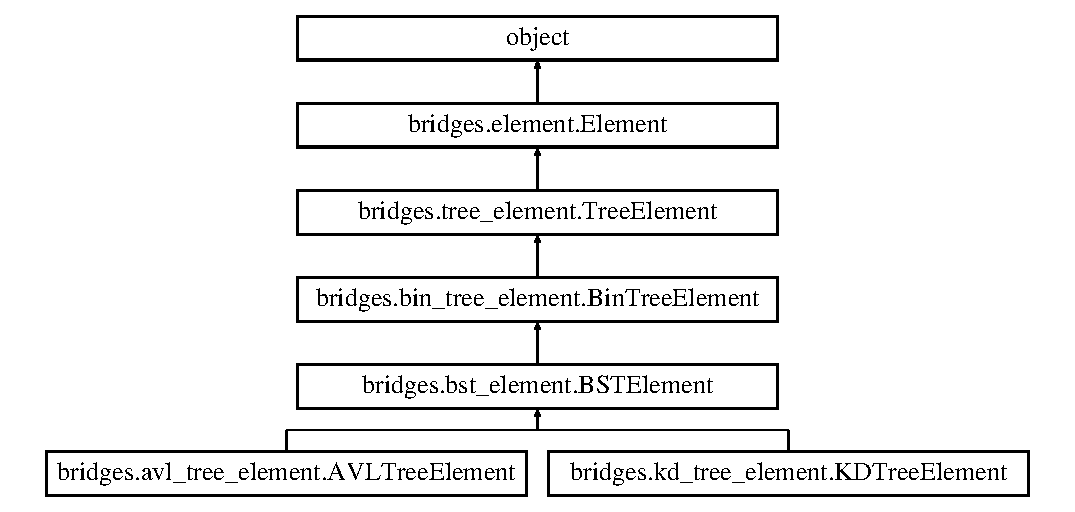
\includegraphics[height=5.000000cm]{classbridges_1_1bin__tree__element_1_1_bin_tree_element}
\end{center}
\end{figure}


\subsection{Detailed Description}
This class is extended from the Tree\+Element class and can be used to create binary tree element objects. 

The Bin\+Tree element class is the building block for creating binary tree structures. It contains two children (viz., left, right).

\hyperlink{classbridges_1_1bin__tree__element_1_1_bin_tree_element}{Bin\+Tree\+Element} contains a visualizer (Element\+Visualizer) object for setting visual attributes (color, shape, opacity, size), necessary for displaying them in a web browser.

Elements also have a Link\+Visualizer object, that is used when they are linked to another element, appropriate for setting link attributes, for instance, between the current element and its left or right child

\begin{DoxyAuthor}{Author}
Kalpathi Subramanian, Mihai Mehedint, Matthew Mc\+Quaigue
\end{DoxyAuthor}
\begin{DoxyDate}{Date}
2018, 7/23/19, 1/6/21
\end{DoxyDate}
\begin{DoxySeeAlso}{See also}
Binary tree tutorial, \href{http://bridgesuncc.github.io/tutorials/BinTree.html}{\tt http\+://bridgesuncc.\+github.\+io/tutorials/\+Bin\+Tree.\+html} 
\end{DoxySeeAlso}
\subsection*{Public Member Functions}
\begin{DoxyCompactItemize}
\item 
def \hyperlink{classbridges_1_1bin__tree__element_1_1_bin_tree_element_ae08e007089e36e3128f45bb29cd001ec}{\+\_\+\+\_\+init\+\_\+\+\_\+} (self, kwargs)
\begin{DoxyCompactList}\small\item\em Constructor for an empty Binary Tree Element. \end{DoxyCompactList}\item 
def \hyperlink{classbridges_1_1bin__tree__element_1_1_bin_tree_element_a974adfbdb569d77586ecf145197b448b}{get\+\_\+data\+\_\+structure\+\_\+type} (self)
\begin{DoxyCompactList}\small\item\em Get the data structure type. \end{DoxyCompactList}\item 
def \hyperlink{classbridges_1_1bin__tree__element_1_1_bin_tree_element_adb99f8052ef772be4c280970e47e6e0d}{left} (self)
\begin{DoxyCompactList}\small\item\em Getter for the left element for the binary tree. \end{DoxyCompactList}\item 
def \hyperlink{classbridges_1_1bin__tree__element_1_1_bin_tree_element_a8c3fb48d81700421f87a439b030d34fa}{left} (self, l)
\begin{DoxyCompactList}\small\item\em Setter for the left element of a binary tree. \end{DoxyCompactList}\item 
def \hyperlink{classbridges_1_1bin__tree__element_1_1_bin_tree_element_adb7eaa3c67233aa5c368e8907043f451}{right} (self)
\begin{DoxyCompactList}\small\item\em Getter for the right element for the binary tree. \end{DoxyCompactList}\item 
def \hyperlink{classbridges_1_1bin__tree__element_1_1_bin_tree_element_a8a009b8fe2744859abc8bfe89ccce697}{right} (self, r)
\begin{DoxyCompactList}\small\item\em Setter for the right element of a binary tree. \end{DoxyCompactList}\end{DoxyCompactItemize}
\subsection*{Additional Inherited Members}


\subsection{Constructor \& Destructor Documentation}
\mbox{\Hypertarget{classbridges_1_1bin__tree__element_1_1_bin_tree_element_ae08e007089e36e3128f45bb29cd001ec}\label{classbridges_1_1bin__tree__element_1_1_bin_tree_element_ae08e007089e36e3128f45bb29cd001ec}} 
\index{bridges\+::bin\+\_\+tree\+\_\+element\+::\+Bin\+Tree\+Element@{bridges\+::bin\+\_\+tree\+\_\+element\+::\+Bin\+Tree\+Element}!\+\_\+\+\_\+init\+\_\+\+\_\+@{\+\_\+\+\_\+init\+\_\+\+\_\+}}
\index{\+\_\+\+\_\+init\+\_\+\+\_\+@{\+\_\+\+\_\+init\+\_\+\+\_\+}!bridges\+::bin\+\_\+tree\+\_\+element\+::\+Bin\+Tree\+Element@{bridges\+::bin\+\_\+tree\+\_\+element\+::\+Bin\+Tree\+Element}}
\subsubsection{\texorpdfstring{\+\_\+\+\_\+init\+\_\+\+\_\+()}{\_\_init\_\_()}}
{\footnotesize\ttfamily def bridges.\+bin\+\_\+tree\+\_\+element.\+Bin\+Tree\+Element.\+\_\+\+\_\+init\+\_\+\+\_\+ (\begin{DoxyParamCaption}\item[{}]{self,  }\item[{}]{kwargs,  }\item[{}]{None }\end{DoxyParamCaption})}



Constructor for an empty Binary Tree Element. 


\begin{DoxyParams}{Parameters}
{\em label} & The label for the tree element that is displayed in the visualization \\
\hline
{\em e} & the generic object that the binary tree element will hold \\
\hline
{\em left} & the binary tree element assigned to child 0 \\
\hline
{\em right} & the binary tree element assigned to child 1 \\
\hline
\end{DoxyParams}
\begin{DoxyReturn}{Returns}


None 
\end{DoxyReturn}


\subsection{Member Function Documentation}
\mbox{\Hypertarget{classbridges_1_1bin__tree__element_1_1_bin_tree_element_a974adfbdb569d77586ecf145197b448b}\label{classbridges_1_1bin__tree__element_1_1_bin_tree_element_a974adfbdb569d77586ecf145197b448b}} 
\index{bridges\+::bin\+\_\+tree\+\_\+element\+::\+Bin\+Tree\+Element@{bridges\+::bin\+\_\+tree\+\_\+element\+::\+Bin\+Tree\+Element}!get\+\_\+data\+\_\+structure\+\_\+type@{get\+\_\+data\+\_\+structure\+\_\+type}}
\index{get\+\_\+data\+\_\+structure\+\_\+type@{get\+\_\+data\+\_\+structure\+\_\+type}!bridges\+::bin\+\_\+tree\+\_\+element\+::\+Bin\+Tree\+Element@{bridges\+::bin\+\_\+tree\+\_\+element\+::\+Bin\+Tree\+Element}}
\subsubsection{\texorpdfstring{get\+\_\+data\+\_\+structure\+\_\+type()}{get\_data\_structure\_type()}}
{\footnotesize\ttfamily def bridges.\+bin\+\_\+tree\+\_\+element.\+Bin\+Tree\+Element.\+get\+\_\+data\+\_\+structure\+\_\+type (\begin{DoxyParamCaption}\item[{}]{self,  }\item[{}]{str }\end{DoxyParamCaption})}



Get the data structure type. 

\begin{DoxyReturn}{Returns}


str representing the data structure type 
\end{DoxyReturn}
\mbox{\Hypertarget{classbridges_1_1bin__tree__element_1_1_bin_tree_element_adb99f8052ef772be4c280970e47e6e0d}\label{classbridges_1_1bin__tree__element_1_1_bin_tree_element_adb99f8052ef772be4c280970e47e6e0d}} 
\index{bridges\+::bin\+\_\+tree\+\_\+element\+::\+Bin\+Tree\+Element@{bridges\+::bin\+\_\+tree\+\_\+element\+::\+Bin\+Tree\+Element}!left@{left}}
\index{left@{left}!bridges\+::bin\+\_\+tree\+\_\+element\+::\+Bin\+Tree\+Element@{bridges\+::bin\+\_\+tree\+\_\+element\+::\+Bin\+Tree\+Element}}
\subsubsection{\texorpdfstring{left()}{left()}\hspace{0.1cm}{\footnotesize\ttfamily [1/2]}}
{\footnotesize\ttfamily def bridges.\+bin\+\_\+tree\+\_\+element.\+Bin\+Tree\+Element.\+left (\begin{DoxyParamCaption}\item[{}]{self }\end{DoxyParamCaption})}



Getter for the left element for the binary tree. 

\begin{DoxyReturn}{Returns}


Tree\+Element left child of this element 
\end{DoxyReturn}
\mbox{\Hypertarget{classbridges_1_1bin__tree__element_1_1_bin_tree_element_a8c3fb48d81700421f87a439b030d34fa}\label{classbridges_1_1bin__tree__element_1_1_bin_tree_element_a8c3fb48d81700421f87a439b030d34fa}} 
\index{bridges\+::bin\+\_\+tree\+\_\+element\+::\+Bin\+Tree\+Element@{bridges\+::bin\+\_\+tree\+\_\+element\+::\+Bin\+Tree\+Element}!left@{left}}
\index{left@{left}!bridges\+::bin\+\_\+tree\+\_\+element\+::\+Bin\+Tree\+Element@{bridges\+::bin\+\_\+tree\+\_\+element\+::\+Bin\+Tree\+Element}}
\subsubsection{\texorpdfstring{left()}{left()}\hspace{0.1cm}{\footnotesize\ttfamily [2/2]}}
{\footnotesize\ttfamily def bridges.\+bin\+\_\+tree\+\_\+element.\+Bin\+Tree\+Element.\+left (\begin{DoxyParamCaption}\item[{}]{self,  }\item[{}]{l,  }\item[{}]{None }\end{DoxyParamCaption})}



Setter for the left element of a binary tree. 


\begin{DoxyParams}{Parameters}
{\em l} & the left element to set \\
\hline
\end{DoxyParams}
\begin{DoxyReturn}{Returns}


None 
\end{DoxyReturn}
\mbox{\Hypertarget{classbridges_1_1bin__tree__element_1_1_bin_tree_element_adb7eaa3c67233aa5c368e8907043f451}\label{classbridges_1_1bin__tree__element_1_1_bin_tree_element_adb7eaa3c67233aa5c368e8907043f451}} 
\index{bridges\+::bin\+\_\+tree\+\_\+element\+::\+Bin\+Tree\+Element@{bridges\+::bin\+\_\+tree\+\_\+element\+::\+Bin\+Tree\+Element}!right@{right}}
\index{right@{right}!bridges\+::bin\+\_\+tree\+\_\+element\+::\+Bin\+Tree\+Element@{bridges\+::bin\+\_\+tree\+\_\+element\+::\+Bin\+Tree\+Element}}
\subsubsection{\texorpdfstring{right()}{right()}\hspace{0.1cm}{\footnotesize\ttfamily [1/2]}}
{\footnotesize\ttfamily def bridges.\+bin\+\_\+tree\+\_\+element.\+Bin\+Tree\+Element.\+right (\begin{DoxyParamCaption}\item[{}]{self }\end{DoxyParamCaption})}



Getter for the right element for the binary tree. 

\begin{DoxyReturn}{Returns}


Tree\+Element the right child of this element 
\end{DoxyReturn}
\mbox{\Hypertarget{classbridges_1_1bin__tree__element_1_1_bin_tree_element_a8a009b8fe2744859abc8bfe89ccce697}\label{classbridges_1_1bin__tree__element_1_1_bin_tree_element_a8a009b8fe2744859abc8bfe89ccce697}} 
\index{bridges\+::bin\+\_\+tree\+\_\+element\+::\+Bin\+Tree\+Element@{bridges\+::bin\+\_\+tree\+\_\+element\+::\+Bin\+Tree\+Element}!right@{right}}
\index{right@{right}!bridges\+::bin\+\_\+tree\+\_\+element\+::\+Bin\+Tree\+Element@{bridges\+::bin\+\_\+tree\+\_\+element\+::\+Bin\+Tree\+Element}}
\subsubsection{\texorpdfstring{right()}{right()}\hspace{0.1cm}{\footnotesize\ttfamily [2/2]}}
{\footnotesize\ttfamily def bridges.\+bin\+\_\+tree\+\_\+element.\+Bin\+Tree\+Element.\+right (\begin{DoxyParamCaption}\item[{}]{self,  }\item[{}]{r,  }\item[{}]{None }\end{DoxyParamCaption})}



Setter for the right element of a binary tree. 


\begin{DoxyParams}{Parameters}
{\em r} & the right element to set \\
\hline
\end{DoxyParams}
\begin{DoxyReturn}{Returns}


None 
\end{DoxyReturn}


The documentation for this class was generated from the following file\+:\begin{DoxyCompactItemize}
\item 
/home/erik/work/bridges/bridges-\/python/bridges/\hyperlink{bin__tree__element_8py}{bin\+\_\+tree\+\_\+element.\+py}\end{DoxyCompactItemize}

\hypertarget{classbridges_1_1bridges_1_1_bridges}{}\doxysection{bridges.\+bridges.\+Bridges Class Reference}
\label{classbridges_1_1bridges_1_1_bridges}\index{bridges.bridges.Bridges@{bridges.bridges.Bridges}}


\doxysubsection{Detailed Description}
The bridges class is the main class that provides interfaces to datasets, maintains user and assignment information, and connects to the bridges server. 

The bridges class is responsible for initializing the bridges system, specifying parameters (user id, assignment id, title, description, data structure type, etc) for the student assignment, generating the data structure representation and transmission to the bridges server. In addition, it provides interfaces to a number of real-\/world datasets, that makes it easy to access the data for use algorithms/data structure assignments. ~\newline


Datasets. The datasets that are currently supported through the BRIDGES API include USGS Earthquake Data, IMDB Actor/\+Movie Data (2 versions), Gutenberg Book Collection Meta Data, a Video Game Dataset, Shakespeare Dataset, Open\+Street\+Map and Elevation map data. More information is found in the respective methods (below) and at \href{https://bridgesuncc.github.io/datasets.html}{\texttt{ https\+://bridgesuncc.\+github.\+io/datasets.\+html}} 

A typical bridges program includes creating the bridges object, followed by creation of the data structure by the user, assigning visual attributes to elements of the data structure, followed by specification of teh data structure type and the call to visualize the data structure (bridges\+::set\+Data\+Structure() and \mbox{\hyperlink{classbridges_1_1bridges_1_1_bridges_a822a7338e4dce27f7d8d0d322bdace08}{visualize()}} methods).

\begin{DoxyAuthor}{Author}
Sean Gallagher, Kalpathi Subramanaian, Mihai Mehedint, David Burlinson, Matthew Mcquaigue, Erik Saule, Jamie Payton
\end{DoxyAuthor}
\begin{DoxyDate}{Date}
2015, 2016, 2017, 2018, 2019, 2020, 2021 
\end{DoxyDate}
\doxysubsection*{Public Member Functions}
\begin{DoxyCompactItemize}
\item 
\mbox{[}float\mbox{]} \mbox{\hyperlink{classbridges_1_1bridges_1_1_bridges_abe7d2ce9cd70820a94914b8b2964b215}{window}} (self)
\begin{DoxyCompactList}\small\item\em This function returns the current window size. \end{DoxyCompactList}\item 
None \mbox{\hyperlink{classbridges_1_1bridges_1_1_bridges_a0bec2e26f9b318f4eb89ed7281565771}{window}} (self, \mbox{[}float\mbox{]} value)
\begin{DoxyCompactList}\small\item\em This function sets the current window size that will rendered by default in the view. \end{DoxyCompactList}\item 
def \mbox{\hyperlink{classbridges_1_1bridges_1_1_bridges_af40aff29a2bc4efbaeb4186275fe7480}{\+\_\+\+\_\+init\+\_\+\+\_\+}} (self, assignment, username=None, appl\+\_\+id=None)
\begin{DoxyCompactList}\small\item\em \mbox{\hyperlink{classbridges_1_1bridges_1_1_bridges}{Bridges}} constructor. \end{DoxyCompactList}\item 
def \mbox{\hyperlink{classbridges_1_1bridges_1_1_bridges_a868f02fa66c87c1a1fc7bd6fbc799291}{set\+\_\+data\+\_\+structure}} (self, ds)
\begin{DoxyCompactList}\small\item\em Set the data structure type. \end{DoxyCompactList}\item 
def \mbox{\hyperlink{classbridges_1_1bridges_1_1_bridges_ab50d018b5178ca33de24157b7b6de285}{set\+\_\+visualize\+\_\+\+JSON}} (self, flag)
\begin{DoxyCompactList}\small\item\em This method controls if the data structure\textquotesingle{}s JSON representation is printed to the console or not. \end{DoxyCompactList}\item 
def \mbox{\hyperlink{classbridges_1_1bridges_1_1_bridges_affea08c46fe175e8ed319b14db319fb1}{post\+\_\+visualization\+\_\+link}} (self, flag)
\begin{DoxyCompactList}\small\item\em This method controls (with a flag) if the visualization url is printed to the console or not. \end{DoxyCompactList}\item 
None \mbox{\hyperlink{classbridges_1_1bridges_1_1_bridges_a822a7338e4dce27f7d8d0d322bdace08}{visualize}} (self)
\begin{DoxyCompactList}\small\item\em Method for generating the representation of the data structure in the form of JSON and sends the information to the bridges server for generating the visualization. \end{DoxyCompactList}\item 
def \mbox{\hyperlink{classbridges_1_1bridges_1_1_bridges_add46441bec1c93095c48adc724b90e12}{set\+\_\+assignment}} (self, assignment)
\begin{DoxyCompactList}\small\item\em Setter for assignment id (must be positive) \end{DoxyCompactList}\item 
str \mbox{\hyperlink{classbridges_1_1bridges_1_1_bridges_ae74fd60689c1cb3088c80e6097d14e73}{get\+\_\+assignment}} (self)
\begin{DoxyCompactList}\small\item\em Getter for the assignment id. \end{DoxyCompactList}\item 
None \mbox{\hyperlink{classbridges_1_1bridges_1_1_bridges_a46ecfa60298f97bd7605f1e224cfab10}{set\+\_\+title}} (self, title)
\begin{DoxyCompactList}\small\item\em Setter for the title of the bridges visualization. \end{DoxyCompactList}\item 
None \mbox{\hyperlink{classbridges_1_1bridges_1_1_bridges_ac61a47f230c8f96f85d810498fad8b97}{set\+\_\+description}} (self, description)
\begin{DoxyCompactList}\small\item\em Setter for the description of the bridges visualization. \end{DoxyCompactList}\item 
def \mbox{\hyperlink{classbridges_1_1bridges_1_1_bridges_ae9ed34b5878d9d120949da0b7e4d2911}{set\+\_\+map\+\_\+overlay}} (self, flag)
\begin{DoxyCompactList}\small\item\em Setter for if the visualization will have a map overlay. \end{DoxyCompactList}\item 
def \mbox{\hyperlink{classbridges_1_1bridges_1_1_bridges_a6bc905490b1995234f88f47af9aa8a17}{set\+\_\+coord\+\_\+system\+\_\+type}} (self, coord)
\begin{DoxyCompactList}\small\item\em Setter for the coordinate system type to use in the visualization. \end{DoxyCompactList}\item 
\mbox{\hyperlink{classbridges_1_1color__grid_1_1_color_grid}{Color\+Grid}} \mbox{\hyperlink{classbridges_1_1bridges_1_1_bridges_a0f809dc3197c139c4e3d178c89b2fa46}{get\+\_\+color\+\_\+grid\+\_\+from\+\_\+assignment}} (self, str user, int assignment, int subassignment=0)
\begin{DoxyCompactList}\small\item\em Reconstruct a Color\+Grid from an existing Color\+Grid on the bridges server. \end{DoxyCompactList}\item 
def \mbox{\hyperlink{classbridges_1_1bridges_1_1_bridges_a3f97735d336faf40585e99362d64a3ee}{set\+\_\+username}} (self, username)
\begin{DoxyCompactList}\small\item\em Setter for username (must be a string) \end{DoxyCompactList}\item 
def \mbox{\hyperlink{classbridges_1_1bridges_1_1_bridges_abf6fdb19db336c2ed14987fdd89d65fe}{get\+\_\+username}} (self)
\begin{DoxyCompactList}\small\item\em Getter for the assignment user name (BRIDGES credentials) \end{DoxyCompactList}\item 
def \mbox{\hyperlink{classbridges_1_1bridges_1_1_bridges_a94f39f11368031ad33800aac0bac2f7d}{get\+\_\+assignment\+\_\+id}} (self)
\begin{DoxyCompactList}\small\item\em Getter for the assignment number. \end{DoxyCompactList}\item 
def \mbox{\hyperlink{classbridges_1_1bridges_1_1_bridges_a5841bc54e3663249e76f4b34f5a3a593}{set\+\_\+key}} (self, apikey)
\begin{DoxyCompactList}\small\item\em Setter for API Key (BRIDGES Credentials) \end{DoxyCompactList}\item 
def \mbox{\hyperlink{classbridges_1_1bridges_1_1_bridges_afcdb0291c535b41fb7be31eaf5bf3677}{get\+\_\+key}} (self)
\begin{DoxyCompactList}\small\item\em Getter for the API key (BRIDGES credentials) \end{DoxyCompactList}\item 
None \mbox{\hyperlink{classbridges_1_1bridges_1_1_bridges_ad58c9e53347c301fbf247b5912715166}{set\+\_\+server\+\_\+url}} (self, str server\+\_\+url)
\begin{DoxyCompactList}\small\item\em Sets url for the output of the visualize method. \end{DoxyCompactList}\end{DoxyCompactItemize}
\doxysubsection*{Public Attributes}
\begin{DoxyCompactItemize}
\item 
\mbox{\hyperlink{classbridges_1_1bridges_1_1_bridges_a1c02ee44e7a4a3ee2f7d9c7d7da7d09f}{connector}}
\item 
\mbox{\hyperlink{classbridges_1_1bridges_1_1_bridges_a7a6f25612be64d4f3e203d7d37cb4da4}{ds\+\_\+handle}}
\item 
\mbox{\hyperlink{classbridges_1_1bridges_1_1_bridges_a5ca152bf3830e2be1f72247463916f82}{vis\+\_\+type}}
\end{DoxyCompactItemize}


\doxysubsection{Constructor \& Destructor Documentation}
\mbox{\Hypertarget{classbridges_1_1bridges_1_1_bridges_af40aff29a2bc4efbaeb4186275fe7480}\label{classbridges_1_1bridges_1_1_bridges_af40aff29a2bc4efbaeb4186275fe7480}} 
\index{bridges.bridges.Bridges@{bridges.bridges.Bridges}!\_\_init\_\_@{\_\_init\_\_}}
\index{\_\_init\_\_@{\_\_init\_\_}!bridges.bridges.Bridges@{bridges.bridges.Bridges}}
\doxysubsubsection{\texorpdfstring{\_\_init\_\_()}{\_\_init\_\_()}}
{\footnotesize\ttfamily def bridges.\+bridges.\+Bridges.\+\_\+\+\_\+init\+\_\+\+\_\+ (\begin{DoxyParamCaption}\item[{}]{self,  }\item[{}]{assignment,  }\item[{}]{username = {\ttfamily None},  }\item[{}]{appl\+\_\+id = {\ttfamily None} }\end{DoxyParamCaption})}



\mbox{\hyperlink{classbridges_1_1bridges_1_1_bridges}{Bridges}} constructor. 

\begin{DoxyVerb}       (int) assignment: the number your bridges assignment will have
       (str) username: your bridges username, optional if BRIDGES_USER_NAME in env
       (str) appl_id: your appl authentication key from bridges acc, optional if BRIDGES_API_KEY in env
\end{DoxyVerb}
 \begin{DoxyReturn}{Returns}


None 
\end{DoxyReturn}


\doxysubsection{Member Function Documentation}
\mbox{\Hypertarget{classbridges_1_1bridges_1_1_bridges_ae74fd60689c1cb3088c80e6097d14e73}\label{classbridges_1_1bridges_1_1_bridges_ae74fd60689c1cb3088c80e6097d14e73}} 
\index{bridges.bridges.Bridges@{bridges.bridges.Bridges}!get\_assignment@{get\_assignment}}
\index{get\_assignment@{get\_assignment}!bridges.bridges.Bridges@{bridges.bridges.Bridges}}
\doxysubsubsection{\texorpdfstring{get\_assignment()}{get\_assignment()}}
{\footnotesize\ttfamily  str bridges.\+bridges.\+Bridges.\+get\+\_\+assignment (\begin{DoxyParamCaption}\item[{}]{self }\end{DoxyParamCaption})}



Getter for the assignment id. 

\begin{DoxyReturn}{Returns}


str representing the full assignment id including subassignment aspect 
\end{DoxyReturn}
\mbox{\Hypertarget{classbridges_1_1bridges_1_1_bridges_a94f39f11368031ad33800aac0bac2f7d}\label{classbridges_1_1bridges_1_1_bridges_a94f39f11368031ad33800aac0bac2f7d}} 
\index{bridges.bridges.Bridges@{bridges.bridges.Bridges}!get\_assignment\_id@{get\_assignment\_id}}
\index{get\_assignment\_id@{get\_assignment\_id}!bridges.bridges.Bridges@{bridges.bridges.Bridges}}
\doxysubsubsection{\texorpdfstring{get\_assignment\_id()}{get\_assignment\_id()}}
{\footnotesize\ttfamily def bridges.\+bridges.\+Bridges.\+get\+\_\+assignment\+\_\+id (\begin{DoxyParamCaption}\item[{}]{self }\end{DoxyParamCaption})}



Getter for the assignment number. 

\begin{DoxyReturn}{Returns}


int assignment number 
\end{DoxyReturn}
\mbox{\Hypertarget{classbridges_1_1bridges_1_1_bridges_a0f809dc3197c139c4e3d178c89b2fa46}\label{classbridges_1_1bridges_1_1_bridges_a0f809dc3197c139c4e3d178c89b2fa46}} 
\index{bridges.bridges.Bridges@{bridges.bridges.Bridges}!get\_color\_grid\_from\_assignment@{get\_color\_grid\_from\_assignment}}
\index{get\_color\_grid\_from\_assignment@{get\_color\_grid\_from\_assignment}!bridges.bridges.Bridges@{bridges.bridges.Bridges}}
\doxysubsubsection{\texorpdfstring{get\_color\_grid\_from\_assignment()}{get\_color\_grid\_from\_assignment()}}
{\footnotesize\ttfamily  \mbox{\hyperlink{classbridges_1_1color__grid_1_1_color_grid}{Color\+Grid}} bridges.\+bridges.\+Bridges.\+get\+\_\+color\+\_\+grid\+\_\+from\+\_\+assignment (\begin{DoxyParamCaption}\item[{}]{self,  }\item[{str}]{user,  }\item[{int}]{assignment,  }\item[{int }]{subassignment = {\ttfamily 0} }\end{DoxyParamCaption})}



Reconstruct a Color\+Grid from an existing Color\+Grid on the bridges server. 


\begin{DoxyParams}{Parameters}
{\em user} & the name of the user who uploaded the assignment \\
\hline
{\em assignment} & the ID of the assignment to get \\
\hline
{\em subassignment} & the ID of the subassignment to get (default 0) \\
\hline
\end{DoxyParams}
\begin{DoxyReturn}{Returns}


Color\+Grid the Color\+Grid stored in the bridges server 
\end{DoxyReturn}
\mbox{\Hypertarget{classbridges_1_1bridges_1_1_bridges_afcdb0291c535b41fb7be31eaf5bf3677}\label{classbridges_1_1bridges_1_1_bridges_afcdb0291c535b41fb7be31eaf5bf3677}} 
\index{bridges.bridges.Bridges@{bridges.bridges.Bridges}!get\_key@{get\_key}}
\index{get\_key@{get\_key}!bridges.bridges.Bridges@{bridges.bridges.Bridges}}
\doxysubsubsection{\texorpdfstring{get\_key()}{get\_key()}}
{\footnotesize\ttfamily def bridges.\+bridges.\+Bridges.\+get\+\_\+key (\begin{DoxyParamCaption}\item[{}]{self }\end{DoxyParamCaption})}



Getter for the API key (BRIDGES credentials) 

\begin{DoxyReturn}{Returns}


str user\textquotesingle{}s API key 
\end{DoxyReturn}
\mbox{\Hypertarget{classbridges_1_1bridges_1_1_bridges_abf6fdb19db336c2ed14987fdd89d65fe}\label{classbridges_1_1bridges_1_1_bridges_abf6fdb19db336c2ed14987fdd89d65fe}} 
\index{bridges.bridges.Bridges@{bridges.bridges.Bridges}!get\_username@{get\_username}}
\index{get\_username@{get\_username}!bridges.bridges.Bridges@{bridges.bridges.Bridges}}
\doxysubsubsection{\texorpdfstring{get\_username()}{get\_username()}}
{\footnotesize\ttfamily def bridges.\+bridges.\+Bridges.\+get\+\_\+username (\begin{DoxyParamCaption}\item[{}]{self }\end{DoxyParamCaption})}



Getter for the assignment user name (BRIDGES credentials) 

\begin{DoxyReturn}{Returns}


str user name 
\end{DoxyReturn}
\mbox{\Hypertarget{classbridges_1_1bridges_1_1_bridges_affea08c46fe175e8ed319b14db319fb1}\label{classbridges_1_1bridges_1_1_bridges_affea08c46fe175e8ed319b14db319fb1}} 
\index{bridges.bridges.Bridges@{bridges.bridges.Bridges}!post\_visualization\_link@{post\_visualization\_link}}
\index{post\_visualization\_link@{post\_visualization\_link}!bridges.bridges.Bridges@{bridges.bridges.Bridges}}
\doxysubsubsection{\texorpdfstring{post\_visualization\_link()}{post\_visualization\_link()}}
{\footnotesize\ttfamily def bridges.\+bridges.\+Bridges.\+post\+\_\+visualization\+\_\+link (\begin{DoxyParamCaption}\item[{}]{self,  }\item[{}]{flag }\end{DoxyParamCaption})}



This method controls (with a flag) if the visualization url is printed to the console or not. 


\begin{DoxyParams}{Parameters}
{\em flag} & flag that controls if the url to the visualization is output to console \\
\hline
\end{DoxyParams}
\mbox{\Hypertarget{classbridges_1_1bridges_1_1_bridges_add46441bec1c93095c48adc724b90e12}\label{classbridges_1_1bridges_1_1_bridges_add46441bec1c93095c48adc724b90e12}} 
\index{bridges.bridges.Bridges@{bridges.bridges.Bridges}!set\_assignment@{set\_assignment}}
\index{set\_assignment@{set\_assignment}!bridges.bridges.Bridges@{bridges.bridges.Bridges}}
\doxysubsubsection{\texorpdfstring{set\_assignment()}{set\_assignment()}}
{\footnotesize\ttfamily def bridges.\+bridges.\+Bridges.\+set\+\_\+assignment (\begin{DoxyParamCaption}\item[{}]{self,  }\item[{}]{assignment }\end{DoxyParamCaption})}



Setter for assignment id (must be positive) 


\begin{DoxyParams}{Parameters}
{\em assignment} & assignment number to be set \\
\hline
\end{DoxyParams}
\begin{DoxyReturn}{Returns}


None 
\end{DoxyReturn}
\mbox{\Hypertarget{classbridges_1_1bridges_1_1_bridges_a6bc905490b1995234f88f47af9aa8a17}\label{classbridges_1_1bridges_1_1_bridges_a6bc905490b1995234f88f47af9aa8a17}} 
\index{bridges.bridges.Bridges@{bridges.bridges.Bridges}!set\_coord\_system\_type@{set\_coord\_system\_type}}
\index{set\_coord\_system\_type@{set\_coord\_system\_type}!bridges.bridges.Bridges@{bridges.bridges.Bridges}}
\doxysubsubsection{\texorpdfstring{set\_coord\_system\_type()}{set\_coord\_system\_type()}}
{\footnotesize\ttfamily def bridges.\+bridges.\+Bridges.\+set\+\_\+coord\+\_\+system\+\_\+type (\begin{DoxyParamCaption}\item[{}]{self,  }\item[{}]{coord }\end{DoxyParamCaption})}



Setter for the coordinate system type to use in the visualization. 


\begin{DoxyParams}{Parameters}
{\em coord} & coordinate system type (used in map overlays (can be \char`\"{}cartesian\char`\"{}, \char`\"{}albersusa\char`\"{}, \char`\"{}equirectangular\char`\"{}) \\
\hline
\end{DoxyParams}
\mbox{\Hypertarget{classbridges_1_1bridges_1_1_bridges_a868f02fa66c87c1a1fc7bd6fbc799291}\label{classbridges_1_1bridges_1_1_bridges_a868f02fa66c87c1a1fc7bd6fbc799291}} 
\index{bridges.bridges.Bridges@{bridges.bridges.Bridges}!set\_data\_structure@{set\_data\_structure}}
\index{set\_data\_structure@{set\_data\_structure}!bridges.bridges.Bridges@{bridges.bridges.Bridges}}
\doxysubsubsection{\texorpdfstring{set\_data\_structure()}{set\_data\_structure()}}
{\footnotesize\ttfamily def bridges.\+bridges.\+Bridges.\+set\+\_\+data\+\_\+structure (\begin{DoxyParamCaption}\item[{}]{self,  }\item[{}]{ds }\end{DoxyParamCaption})}



Set the data structure type. 

This method sets the handle to the current data structure; this can be an array, the head of a linked list, root of a tree structure, a graph Arrays of upto 3 dimensions are suppported. It can be any of the data structures supported by BRIDGES. Polymorphism and type casting is used to determine the actual data structure and extract its representtion.


\begin{DoxyParams}{Parameters}
{\em ds} & the data structure to visualize \\
\hline
\end{DoxyParams}
\begin{DoxyReturn}{Returns}


None
\end{DoxyReturn}

\begin{DoxyExceptions}{Exceptions}
{\em Value\+Error} & if it is not a BRIDGES data structure \\
\hline
\end{DoxyExceptions}
\mbox{\Hypertarget{classbridges_1_1bridges_1_1_bridges_ac61a47f230c8f96f85d810498fad8b97}\label{classbridges_1_1bridges_1_1_bridges_ac61a47f230c8f96f85d810498fad8b97}} 
\index{bridges.bridges.Bridges@{bridges.bridges.Bridges}!set\_description@{set\_description}}
\index{set\_description@{set\_description}!bridges.bridges.Bridges@{bridges.bridges.Bridges}}
\doxysubsubsection{\texorpdfstring{set\_description()}{set\_description()}}
{\footnotesize\ttfamily  None bridges.\+bridges.\+Bridges.\+set\+\_\+description (\begin{DoxyParamCaption}\item[{}]{self,  }\item[{}]{description }\end{DoxyParamCaption})}



Setter for the description of the bridges visualization. 

\begin{DoxyVerb}       (str) description: representing the assignment description
\end{DoxyVerb}
 \begin{DoxyReturn}{Returns}


None 
\end{DoxyReturn}
\mbox{\Hypertarget{classbridges_1_1bridges_1_1_bridges_a5841bc54e3663249e76f4b34f5a3a593}\label{classbridges_1_1bridges_1_1_bridges_a5841bc54e3663249e76f4b34f5a3a593}} 
\index{bridges.bridges.Bridges@{bridges.bridges.Bridges}!set\_key@{set\_key}}
\index{set\_key@{set\_key}!bridges.bridges.Bridges@{bridges.bridges.Bridges}}
\doxysubsubsection{\texorpdfstring{set\_key()}{set\_key()}}
{\footnotesize\ttfamily def bridges.\+bridges.\+Bridges.\+set\+\_\+key (\begin{DoxyParamCaption}\item[{}]{self,  }\item[{}]{apikey }\end{DoxyParamCaption})}



Setter for API Key (BRIDGES Credentials) 


\begin{DoxyParams}{Parameters}
{\em apikey} & api key to be set \\
\hline
\end{DoxyParams}
\begin{DoxyReturn}{Returns}


None 
\end{DoxyReturn}
\mbox{\Hypertarget{classbridges_1_1bridges_1_1_bridges_ae9ed34b5878d9d120949da0b7e4d2911}\label{classbridges_1_1bridges_1_1_bridges_ae9ed34b5878d9d120949da0b7e4d2911}} 
\index{bridges.bridges.Bridges@{bridges.bridges.Bridges}!set\_map\_overlay@{set\_map\_overlay}}
\index{set\_map\_overlay@{set\_map\_overlay}!bridges.bridges.Bridges@{bridges.bridges.Bridges}}
\doxysubsubsection{\texorpdfstring{set\_map\_overlay()}{set\_map\_overlay()}}
{\footnotesize\ttfamily def bridges.\+bridges.\+Bridges.\+set\+\_\+map\+\_\+overlay (\begin{DoxyParamCaption}\item[{}]{self,  }\item[{}]{flag }\end{DoxyParamCaption})}



Setter for if the visualization will have a map overlay. 

\begin{DoxyVerb}       (bool) flag: boolean for if map overlay
\end{DoxyVerb}
 \begin{DoxyReturn}{Returns}


None 
\end{DoxyReturn}
\mbox{\Hypertarget{classbridges_1_1bridges_1_1_bridges_ad58c9e53347c301fbf247b5912715166}\label{classbridges_1_1bridges_1_1_bridges_ad58c9e53347c301fbf247b5912715166}} 
\index{bridges.bridges.Bridges@{bridges.bridges.Bridges}!set\_server\_url@{set\_server\_url}}
\index{set\_server\_url@{set\_server\_url}!bridges.bridges.Bridges@{bridges.bridges.Bridges}}
\doxysubsubsection{\texorpdfstring{set\_server\_url()}{set\_server\_url()}}
{\footnotesize\ttfamily  None bridges.\+bridges.\+Bridges.\+set\+\_\+server\+\_\+url (\begin{DoxyParamCaption}\item[{}]{self,  }\item[{str}]{server\+\_\+url }\end{DoxyParamCaption})}



Sets url for the output of the visualize method. 


\begin{DoxyParams}{Parameters}
{\em server\+\_\+url} & string, must be one of \{live, clone, local, games\} \\
\hline
\end{DoxyParams}
\begin{DoxyReturn}{Returns}


None 
\end{DoxyReturn}
\mbox{\Hypertarget{classbridges_1_1bridges_1_1_bridges_a46ecfa60298f97bd7605f1e224cfab10}\label{classbridges_1_1bridges_1_1_bridges_a46ecfa60298f97bd7605f1e224cfab10}} 
\index{bridges.bridges.Bridges@{bridges.bridges.Bridges}!set\_title@{set\_title}}
\index{set\_title@{set\_title}!bridges.bridges.Bridges@{bridges.bridges.Bridges}}
\doxysubsubsection{\texorpdfstring{set\_title()}{set\_title()}}
{\footnotesize\ttfamily  None bridges.\+bridges.\+Bridges.\+set\+\_\+title (\begin{DoxyParamCaption}\item[{}]{self,  }\item[{}]{title }\end{DoxyParamCaption})}



Setter for the title of the bridges visualization. 

\begin{DoxyVerb}       (str) title: representing the title
\end{DoxyVerb}
 \begin{DoxyReturn}{Returns}


None 
\end{DoxyReturn}
\mbox{\Hypertarget{classbridges_1_1bridges_1_1_bridges_a3f97735d336faf40585e99362d64a3ee}\label{classbridges_1_1bridges_1_1_bridges_a3f97735d336faf40585e99362d64a3ee}} 
\index{bridges.bridges.Bridges@{bridges.bridges.Bridges}!set\_username@{set\_username}}
\index{set\_username@{set\_username}!bridges.bridges.Bridges@{bridges.bridges.Bridges}}
\doxysubsubsection{\texorpdfstring{set\_username()}{set\_username()}}
{\footnotesize\ttfamily def bridges.\+bridges.\+Bridges.\+set\+\_\+username (\begin{DoxyParamCaption}\item[{}]{self,  }\item[{}]{username }\end{DoxyParamCaption})}



Setter for username (must be a string) 


\begin{DoxyParams}{Parameters}
{\em username} & username to be set \\
\hline
\end{DoxyParams}
\begin{DoxyReturn}{Returns}


None 
\end{DoxyReturn}
\mbox{\Hypertarget{classbridges_1_1bridges_1_1_bridges_ab50d018b5178ca33de24157b7b6de285}\label{classbridges_1_1bridges_1_1_bridges_ab50d018b5178ca33de24157b7b6de285}} 
\index{bridges.bridges.Bridges@{bridges.bridges.Bridges}!set\_visualize\_JSON@{set\_visualize\_JSON}}
\index{set\_visualize\_JSON@{set\_visualize\_JSON}!bridges.bridges.Bridges@{bridges.bridges.Bridges}}
\doxysubsubsection{\texorpdfstring{set\_visualize\_JSON()}{set\_visualize\_JSON()}}
{\footnotesize\ttfamily def bridges.\+bridges.\+Bridges.\+set\+\_\+visualize\+\_\+\+JSON (\begin{DoxyParamCaption}\item[{}]{self,  }\item[{}]{flag }\end{DoxyParamCaption})}



This method controls if the data structure\textquotesingle{}s JSON representation is printed to the console or not. 


\begin{DoxyParams}{Parameters}
{\em flag} & flag that controls if the JSON of the data structure representation is output to console \\
\hline
\end{DoxyParams}
\begin{DoxyReturn}{Returns}


None 
\end{DoxyReturn}
\mbox{\Hypertarget{classbridges_1_1bridges_1_1_bridges_a822a7338e4dce27f7d8d0d322bdace08}\label{classbridges_1_1bridges_1_1_bridges_a822a7338e4dce27f7d8d0d322bdace08}} 
\index{bridges.bridges.Bridges@{bridges.bridges.Bridges}!visualize@{visualize}}
\index{visualize@{visualize}!bridges.bridges.Bridges@{bridges.bridges.Bridges}}
\doxysubsubsection{\texorpdfstring{visualize()}{visualize()}}
{\footnotesize\ttfamily  None bridges.\+bridges.\+Bridges.\+visualize (\begin{DoxyParamCaption}\item[{}]{self }\end{DoxyParamCaption})}



Method for generating the representation of the data structure in the form of JSON and sends the information to the bridges server for generating the visualization. 

\begin{DoxyReturn}{Returns}


None 
\end{DoxyReturn}
\mbox{\Hypertarget{classbridges_1_1bridges_1_1_bridges_abe7d2ce9cd70820a94914b8b2964b215}\label{classbridges_1_1bridges_1_1_bridges_abe7d2ce9cd70820a94914b8b2964b215}} 
\index{bridges.bridges.Bridges@{bridges.bridges.Bridges}!window@{window}}
\index{window@{window}!bridges.bridges.Bridges@{bridges.bridges.Bridges}}
\doxysubsubsection{\texorpdfstring{window()}{window()}\hspace{0.1cm}{\footnotesize\ttfamily [1/2]}}
{\footnotesize\ttfamily  \mbox{[}float\mbox{]} bridges.\+bridges.\+Bridges.\+window (\begin{DoxyParamCaption}\item[{}]{self }\end{DoxyParamCaption})}



This function returns the current window size. 

This only works for graph data types. And the coordinate system need to be set to \char`\"{}window\char`\"{} using \mbox{\hyperlink{classbridges_1_1bridges_1_1_bridges_a6bc905490b1995234f88f47af9aa8a17}{set\+\_\+coord\+\_\+system\+\_\+type()}}, setting this value will set \char`\"{}window\char`\"{} for you. \begin{DoxyReturn}{Returns}
return a list of 4 floats \mbox{[}x1, x2, y1, y2\mbox{]} 
\end{DoxyReturn}
\mbox{\Hypertarget{classbridges_1_1bridges_1_1_bridges_a0bec2e26f9b318f4eb89ed7281565771}\label{classbridges_1_1bridges_1_1_bridges_a0bec2e26f9b318f4eb89ed7281565771}} 
\index{bridges.bridges.Bridges@{bridges.bridges.Bridges}!window@{window}}
\index{window@{window}!bridges.bridges.Bridges@{bridges.bridges.Bridges}}
\doxysubsubsection{\texorpdfstring{window()}{window()}\hspace{0.1cm}{\footnotesize\ttfamily [2/2]}}
{\footnotesize\ttfamily  None bridges.\+bridges.\+Bridges.\+window (\begin{DoxyParamCaption}\item[{}]{self,  }\item[{\mbox{[}float\mbox{]}}]{value }\end{DoxyParamCaption})}



This function sets the current window size that will rendered by default in the view. 

This only works for graph data types. And the coordinate system need to be set to \char`\"{}window\char`\"{} using \mbox{\hyperlink{classbridges_1_1bridges_1_1_bridges_a6bc905490b1995234f88f47af9aa8a17}{set\+\_\+coord\+\_\+system\+\_\+type()}}, setting this value will set \char`\"{}window\char`\"{} for you. 

\doxysubsection{Member Data Documentation}
\mbox{\Hypertarget{classbridges_1_1bridges_1_1_bridges_a1c02ee44e7a4a3ee2f7d9c7d7da7d09f}\label{classbridges_1_1bridges_1_1_bridges_a1c02ee44e7a4a3ee2f7d9c7d7da7d09f}} 
\index{bridges.bridges.Bridges@{bridges.bridges.Bridges}!connector@{connector}}
\index{connector@{connector}!bridges.bridges.Bridges@{bridges.bridges.Bridges}}
\doxysubsubsection{\texorpdfstring{connector}{connector}}
{\footnotesize\ttfamily bridges.\+bridges.\+Bridges.\+connector}

\mbox{\Hypertarget{classbridges_1_1bridges_1_1_bridges_a7a6f25612be64d4f3e203d7d37cb4da4}\label{classbridges_1_1bridges_1_1_bridges_a7a6f25612be64d4f3e203d7d37cb4da4}} 
\index{bridges.bridges.Bridges@{bridges.bridges.Bridges}!ds\_handle@{ds\_handle}}
\index{ds\_handle@{ds\_handle}!bridges.bridges.Bridges@{bridges.bridges.Bridges}}
\doxysubsubsection{\texorpdfstring{ds\_handle}{ds\_handle}}
{\footnotesize\ttfamily bridges.\+bridges.\+Bridges.\+ds\+\_\+handle}

\mbox{\Hypertarget{classbridges_1_1bridges_1_1_bridges_a5ca152bf3830e2be1f72247463916f82}\label{classbridges_1_1bridges_1_1_bridges_a5ca152bf3830e2be1f72247463916f82}} 
\index{bridges.bridges.Bridges@{bridges.bridges.Bridges}!vis\_type@{vis\_type}}
\index{vis\_type@{vis\_type}!bridges.bridges.Bridges@{bridges.bridges.Bridges}}
\doxysubsubsection{\texorpdfstring{vis\_type}{vis\_type}}
{\footnotesize\ttfamily bridges.\+bridges.\+Bridges.\+vis\+\_\+type}



The documentation for this class was generated from the following file\+:\begin{DoxyCompactItemize}
\item 
/\+Users/kalpathi/gr/bridges/client/python/bridges/\mbox{\hyperlink{bridges_8py}{bridges.\+py}}\end{DoxyCompactItemize}

\hypertarget{classbridges_1_1bst__element_1_1_b_s_t_element}{}\doxysection{bridges.\+bst\+\_\+element.\+BSTElement Class Reference}
\label{classbridges_1_1bst__element_1_1_b_s_t_element}\index{bridges.bst\_element.BSTElement@{bridges.bst\_element.BSTElement}}
Inheritance diagram for bridges.\+bst\+\_\+element.\+BSTElement\+:\begin{figure}[H]
\begin{center}
\leavevmode
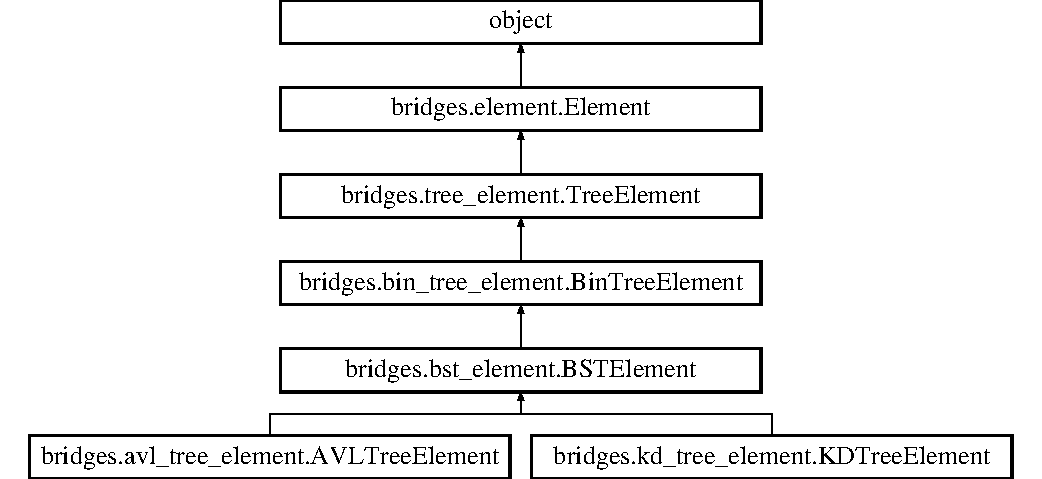
\includegraphics[height=5.000000cm]{classbridges_1_1bst__element_1_1_b_s_t_element}
\end{center}
\end{figure}


\doxysubsection{Detailed Description}
The \mbox{\hyperlink{classbridges_1_1bst__element_1_1_b_s_t_element}{BSTElement}} class is the building block for creating binary search trees. 

The \mbox{\hyperlink{classbridges_1_1bst__element_1_1_b_s_t_element}{BSTElement}} class is the building block for creating binary search tree structures. It contains two children (viz., left, right), and a search key, to be used in search operations .

\mbox{\hyperlink{classbridges_1_1bst__element_1_1_b_s_t_element}{BSTElement}} contains a visualizer (Element\+Visualizer) object for setting visual attributes (color, shape, opacity, size), necessary for displaying them in a web browser.

BST Elements also have a Link\+Visualizer object, that is used when they are linked to another element, appropriate for setting link attributes, for instance, between the current element and its left or right child

\begin{DoxyAuthor}{Author}
Kalpathi Subramanian, Mihai Mehedint, Matthew Mc\+Quaigue
\end{DoxyAuthor}
\begin{DoxyDate}{Date}
6/22/16, 1/7/17, 5/17/17, 7/23/19, 2021
\end{DoxyDate}
This class extends the Bin\+Tree\+Element class by adding a \textquotesingle{}key\textquotesingle{} value for use in a binary search tree implementations.

Binary Search Tree tutorial, \href{https://bridgesuncc.github.io/tutorials/BinarySearchTree.html}{\texttt{ https\+://bridgesuncc.\+github.\+io/tutorials/\+Binary\+Search\+Tree.\+html}} \doxysubsection*{Public Member Functions}
\begin{DoxyCompactItemize}
\item 
None \mbox{\hyperlink{classbridges_1_1bst__element_1_1_b_s_t_element_a0be9b75a1da9322d40811669d13e05a4}{\+\_\+\+\_\+init\+\_\+\+\_\+}} (self, $\ast$$\ast$kwargs)
\begin{DoxyCompactList}\small\item\em Constructor bst element. \end{DoxyCompactList}\item 
str \mbox{\hyperlink{classbridges_1_1bst__element_1_1_b_s_t_element_a8e655e06ba0f77b7e2681b6d291f39de}{get\+\_\+data\+\_\+structure\+\_\+type}} (self)
\begin{DoxyCompactList}\small\item\em Get the data structure representation. \end{DoxyCompactList}\item 
str \mbox{\hyperlink{classbridges_1_1bst__element_1_1_b_s_t_element_ae911a11782ad4623b21781c5eeeb7d39}{key}} (self)
\begin{DoxyCompactList}\small\item\em Getter for the bst element key. \end{DoxyCompactList}\item 
None \mbox{\hyperlink{classbridges_1_1bst__element_1_1_b_s_t_element_a646b48db2f62727bc86b51ed09069155}{key}} (self, str k)
\begin{DoxyCompactList}\small\item\em Setter for the bst element key. \end{DoxyCompactList}\item 
def \mbox{\hyperlink{classbridges_1_1bst__element_1_1_b_s_t_element_adb40ae0f98fe1cb7f153494c544d3f9f}{left}} (self)
\begin{DoxyCompactList}\small\item\em Getter for the left element in BST. \end{DoxyCompactList}\item 
def \mbox{\hyperlink{classbridges_1_1bst__element_1_1_b_s_t_element_a0b45e63b73faabb6b969dd6222e07942}{left}} (self, l)
\begin{DoxyCompactList}\small\item\em Setter for the left element in BST. \end{DoxyCompactList}\item 
def \mbox{\hyperlink{classbridges_1_1bst__element_1_1_b_s_t_element_a3ec82fbc56a5e6309b69d2d963b483fd}{right}} (self)
\begin{DoxyCompactList}\small\item\em Getter for the right child in BST. \end{DoxyCompactList}\item 
def \mbox{\hyperlink{classbridges_1_1bst__element_1_1_b_s_t_element_a978ae0db366dee59703ed266eebca0e9}{right}} (self, r)
\begin{DoxyCompactList}\small\item\em Setter for the right element in BST. \end{DoxyCompactList}\item 
dict \mbox{\hyperlink{classbridges_1_1bst__element_1_1_b_s_t_element_a9d038f191a7cf06e75910463a3aa3b80}{get\+\_\+element\+\_\+representation}} (self)
\begin{DoxyCompactList}\small\item\em Augment the element with the \char`\"{}key\char`\"{} field. \end{DoxyCompactList}\end{DoxyCompactItemize}
\doxysubsection*{Additional Inherited Members}


\doxysubsection{Constructor \& Destructor Documentation}
\mbox{\Hypertarget{classbridges_1_1bst__element_1_1_b_s_t_element_a0be9b75a1da9322d40811669d13e05a4}\label{classbridges_1_1bst__element_1_1_b_s_t_element_a0be9b75a1da9322d40811669d13e05a4}} 
\index{bridges.bst\_element.BSTElement@{bridges.bst\_element.BSTElement}!\_\_init\_\_@{\_\_init\_\_}}
\index{\_\_init\_\_@{\_\_init\_\_}!bridges.bst\_element.BSTElement@{bridges.bst\_element.BSTElement}}
\doxysubsubsection{\texorpdfstring{\_\_init\_\_()}{\_\_init\_\_()}}
{\footnotesize\ttfamily  None bridges.\+bst\+\_\+element.\+BSTElement.\+\_\+\+\_\+init\+\_\+\+\_\+ (\begin{DoxyParamCaption}\item[{}]{self,  }\item[{$\ast$$\ast$}]{kwargs }\end{DoxyParamCaption})}



Constructor bst element. 

\begin{DoxyVerb}       (str) key: The label for the tree element that shows in visualization
       (generic) e: the generic object that the tree element will hold
       (BinTreeElement) left: the tree element assigned to child 0
       (BinTreeElement) right: the tree element assigned to child 1
\end{DoxyVerb}
 \begin{DoxyReturn}{Returns}


None 
\end{DoxyReturn}


Reimplemented from \mbox{\hyperlink{classbridges_1_1bin__tree__element_1_1_bin_tree_element_a4c50812c9a43aa5cd75ccc46b818a8b2}{bridges.\+bin\+\_\+tree\+\_\+element.\+Bin\+Tree\+Element}}.



Reimplemented in \mbox{\hyperlink{classbridges_1_1kd__tree__element_1_1_k_d_tree_element_ad48f0bdabbb21cf83782efc1f8dbc1ed}{bridges.\+kd\+\_\+tree\+\_\+element.\+KDTree\+Element}}.



\doxysubsection{Member Function Documentation}
\mbox{\Hypertarget{classbridges_1_1bst__element_1_1_b_s_t_element_a8e655e06ba0f77b7e2681b6d291f39de}\label{classbridges_1_1bst__element_1_1_b_s_t_element_a8e655e06ba0f77b7e2681b6d291f39de}} 
\index{bridges.bst\_element.BSTElement@{bridges.bst\_element.BSTElement}!get\_data\_structure\_type@{get\_data\_structure\_type}}
\index{get\_data\_structure\_type@{get\_data\_structure\_type}!bridges.bst\_element.BSTElement@{bridges.bst\_element.BSTElement}}
\doxysubsubsection{\texorpdfstring{get\_data\_structure\_type()}{get\_data\_structure\_type()}}
{\footnotesize\ttfamily  str bridges.\+bst\+\_\+element.\+BSTElement.\+get\+\_\+data\+\_\+structure\+\_\+type (\begin{DoxyParamCaption}\item[{}]{self }\end{DoxyParamCaption})}



Get the data structure representation. 

\begin{DoxyReturn}{Returns}


str 
\end{DoxyReturn}


Reimplemented from \mbox{\hyperlink{classbridges_1_1bin__tree__element_1_1_bin_tree_element_a9238744e18486fb8882238394f5efe7c}{bridges.\+bin\+\_\+tree\+\_\+element.\+Bin\+Tree\+Element}}.



Reimplemented in \mbox{\hyperlink{classbridges_1_1kd__tree__element_1_1_k_d_tree_element_a4b38af960542ccc8c3b74d90ee9570e2}{bridges.\+kd\+\_\+tree\+\_\+element.\+KDTree\+Element}}, and \mbox{\hyperlink{classbridges_1_1avl__tree__element_1_1_a_v_l_tree_element_a811dd4cebd36fda6531f6cbeb873c0e5}{bridges.\+avl\+\_\+tree\+\_\+element.\+AVLTree\+Element}}.

\mbox{\Hypertarget{classbridges_1_1bst__element_1_1_b_s_t_element_a9d038f191a7cf06e75910463a3aa3b80}\label{classbridges_1_1bst__element_1_1_b_s_t_element_a9d038f191a7cf06e75910463a3aa3b80}} 
\index{bridges.bst\_element.BSTElement@{bridges.bst\_element.BSTElement}!get\_element\_representation@{get\_element\_representation}}
\index{get\_element\_representation@{get\_element\_representation}!bridges.bst\_element.BSTElement@{bridges.bst\_element.BSTElement}}
\doxysubsubsection{\texorpdfstring{get\_element\_representation()}{get\_element\_representation()}}
{\footnotesize\ttfamily  dict bridges.\+bst\+\_\+element.\+BSTElement.\+get\+\_\+element\+\_\+representation (\begin{DoxyParamCaption}\item[{}]{self }\end{DoxyParamCaption})}



Augment the element with the \char`\"{}key\char`\"{} field. 

\begin{DoxyReturn}{Returns}


dict representing the json of this tree 
\end{DoxyReturn}


Reimplemented from \mbox{\hyperlink{classbridges_1_1element_1_1_element_a511fbc6323616d806ae0ae33010f4654}{bridges.\+element.\+Element}}.



Reimplemented in \mbox{\hyperlink{classbridges_1_1kd__tree__element_1_1_k_d_tree_element_a4e08a6f2e4ff70be2b0dfd6eacdcf10e}{bridges.\+kd\+\_\+tree\+\_\+element.\+KDTree\+Element}}, and \mbox{\hyperlink{classbridges_1_1avl__tree__element_1_1_a_v_l_tree_element_abf8842cb462f1e31f0889d67fb0d70d4}{bridges.\+avl\+\_\+tree\+\_\+element.\+AVLTree\+Element}}.

\mbox{\Hypertarget{classbridges_1_1bst__element_1_1_b_s_t_element_ae911a11782ad4623b21781c5eeeb7d39}\label{classbridges_1_1bst__element_1_1_b_s_t_element_ae911a11782ad4623b21781c5eeeb7d39}} 
\index{bridges.bst\_element.BSTElement@{bridges.bst\_element.BSTElement}!key@{key}}
\index{key@{key}!bridges.bst\_element.BSTElement@{bridges.bst\_element.BSTElement}}
\doxysubsubsection{\texorpdfstring{key()}{key()}\hspace{0.1cm}{\footnotesize\ttfamily [1/2]}}
{\footnotesize\ttfamily  str bridges.\+bst\+\_\+element.\+BSTElement.\+key (\begin{DoxyParamCaption}\item[{}]{self }\end{DoxyParamCaption})}



Getter for the bst element key. 

\begin{DoxyReturn}{Returns}


str the key label 
\end{DoxyReturn}


Reimplemented in \mbox{\hyperlink{classbridges_1_1avl__tree__element_1_1_a_v_l_tree_element_ac830bbf88d156574fd23a8b1eaa6bc69}{bridges.\+avl\+\_\+tree\+\_\+element.\+AVLTree\+Element}}.

\mbox{\Hypertarget{classbridges_1_1bst__element_1_1_b_s_t_element_a646b48db2f62727bc86b51ed09069155}\label{classbridges_1_1bst__element_1_1_b_s_t_element_a646b48db2f62727bc86b51ed09069155}} 
\index{bridges.bst\_element.BSTElement@{bridges.bst\_element.BSTElement}!key@{key}}
\index{key@{key}!bridges.bst\_element.BSTElement@{bridges.bst\_element.BSTElement}}
\doxysubsubsection{\texorpdfstring{key()}{key()}\hspace{0.1cm}{\footnotesize\ttfamily [2/2]}}
{\footnotesize\ttfamily  None bridges.\+bst\+\_\+element.\+BSTElement.\+key (\begin{DoxyParamCaption}\item[{}]{self,  }\item[{str}]{k }\end{DoxyParamCaption})}



Setter for the bst element key. 


\begin{DoxyParams}{Parameters}
{\em k} & the key for the element \\
\hline
\end{DoxyParams}
\begin{DoxyReturn}{Returns}


None 
\end{DoxyReturn}
\mbox{\Hypertarget{classbridges_1_1bst__element_1_1_b_s_t_element_adb40ae0f98fe1cb7f153494c544d3f9f}\label{classbridges_1_1bst__element_1_1_b_s_t_element_adb40ae0f98fe1cb7f153494c544d3f9f}} 
\index{bridges.bst\_element.BSTElement@{bridges.bst\_element.BSTElement}!left@{left}}
\index{left@{left}!bridges.bst\_element.BSTElement@{bridges.bst\_element.BSTElement}}
\doxysubsubsection{\texorpdfstring{left()}{left()}\hspace{0.1cm}{\footnotesize\ttfamily [1/2]}}
{\footnotesize\ttfamily def bridges.\+bst\+\_\+element.\+BSTElement.\+left (\begin{DoxyParamCaption}\item[{}]{self }\end{DoxyParamCaption})}



Getter for the left element in BST. 

\begin{DoxyReturn}{Returns}


\mbox{\hyperlink{classbridges_1_1bst__element_1_1_b_s_t_element}{BSTElement}} the left child of this element 
\end{DoxyReturn}


Reimplemented from \mbox{\hyperlink{classbridges_1_1bin__tree__element_1_1_bin_tree_element_adb99f8052ef772be4c280970e47e6e0d}{bridges.\+bin\+\_\+tree\+\_\+element.\+Bin\+Tree\+Element}}.



Reimplemented in \mbox{\hyperlink{classbridges_1_1kd__tree__element_1_1_k_d_tree_element_afa4f059c61b3cd9460199c9835641db2}{bridges.\+kd\+\_\+tree\+\_\+element.\+KDTree\+Element}}, and \mbox{\hyperlink{classbridges_1_1avl__tree__element_1_1_a_v_l_tree_element_a717696b26736f5c9585fefc7c5ab88f1}{bridges.\+avl\+\_\+tree\+\_\+element.\+AVLTree\+Element}}.

\mbox{\Hypertarget{classbridges_1_1bst__element_1_1_b_s_t_element_a0b45e63b73faabb6b969dd6222e07942}\label{classbridges_1_1bst__element_1_1_b_s_t_element_a0b45e63b73faabb6b969dd6222e07942}} 
\index{bridges.bst\_element.BSTElement@{bridges.bst\_element.BSTElement}!left@{left}}
\index{left@{left}!bridges.bst\_element.BSTElement@{bridges.bst\_element.BSTElement}}
\doxysubsubsection{\texorpdfstring{left()}{left()}\hspace{0.1cm}{\footnotesize\ttfamily [2/2]}}
{\footnotesize\ttfamily def bridges.\+bst\+\_\+element.\+BSTElement.\+left (\begin{DoxyParamCaption}\item[{}]{self,  }\item[{}]{l }\end{DoxyParamCaption})}



Setter for the left element in BST. 


\begin{DoxyParams}{Parameters}
{\em l} & the value for the left child to be set as \\
\hline
\end{DoxyParams}


Reimplemented from \mbox{\hyperlink{classbridges_1_1bin__tree__element_1_1_bin_tree_element_a29dc5b117c65774e756b46de45cd2f20}{bridges.\+bin\+\_\+tree\+\_\+element.\+Bin\+Tree\+Element}}.



Reimplemented in \mbox{\hyperlink{classbridges_1_1avl__tree__element_1_1_a_v_l_tree_element_a5ee29c8a42e07019a77ecd7a2534f8be}{bridges.\+avl\+\_\+tree\+\_\+element.\+AVLTree\+Element}}, and \mbox{\hyperlink{classbridges_1_1kd__tree__element_1_1_k_d_tree_element_a784bad6511dae3a7c769672d2d3af14f}{bridges.\+kd\+\_\+tree\+\_\+element.\+KDTree\+Element}}.

\mbox{\Hypertarget{classbridges_1_1bst__element_1_1_b_s_t_element_a3ec82fbc56a5e6309b69d2d963b483fd}\label{classbridges_1_1bst__element_1_1_b_s_t_element_a3ec82fbc56a5e6309b69d2d963b483fd}} 
\index{bridges.bst\_element.BSTElement@{bridges.bst\_element.BSTElement}!right@{right}}
\index{right@{right}!bridges.bst\_element.BSTElement@{bridges.bst\_element.BSTElement}}
\doxysubsubsection{\texorpdfstring{right()}{right()}\hspace{0.1cm}{\footnotesize\ttfamily [1/2]}}
{\footnotesize\ttfamily def bridges.\+bst\+\_\+element.\+BSTElement.\+right (\begin{DoxyParamCaption}\item[{}]{self }\end{DoxyParamCaption})}



Getter for the right child in BST. 

\begin{DoxyReturn}{Returns}


\mbox{\hyperlink{classbridges_1_1bst__element_1_1_b_s_t_element}{BSTElement}} the right child of the element 
\end{DoxyReturn}


Reimplemented from \mbox{\hyperlink{classbridges_1_1bin__tree__element_1_1_bin_tree_element_adb7eaa3c67233aa5c368e8907043f451}{bridges.\+bin\+\_\+tree\+\_\+element.\+Bin\+Tree\+Element}}.



Reimplemented in \mbox{\hyperlink{classbridges_1_1kd__tree__element_1_1_k_d_tree_element_acbcfa46ba613daaf922d8b632b795a86}{bridges.\+kd\+\_\+tree\+\_\+element.\+KDTree\+Element}}, and \mbox{\hyperlink{classbridges_1_1avl__tree__element_1_1_a_v_l_tree_element_aaab3b79617e7e503b1a7c28069d1eb15}{bridges.\+avl\+\_\+tree\+\_\+element.\+AVLTree\+Element}}.

\mbox{\Hypertarget{classbridges_1_1bst__element_1_1_b_s_t_element_a978ae0db366dee59703ed266eebca0e9}\label{classbridges_1_1bst__element_1_1_b_s_t_element_a978ae0db366dee59703ed266eebca0e9}} 
\index{bridges.bst\_element.BSTElement@{bridges.bst\_element.BSTElement}!right@{right}}
\index{right@{right}!bridges.bst\_element.BSTElement@{bridges.bst\_element.BSTElement}}
\doxysubsubsection{\texorpdfstring{right()}{right()}\hspace{0.1cm}{\footnotesize\ttfamily [2/2]}}
{\footnotesize\ttfamily def bridges.\+bst\+\_\+element.\+BSTElement.\+right (\begin{DoxyParamCaption}\item[{}]{self,  }\item[{}]{r }\end{DoxyParamCaption})}



Setter for the right element in BST. 


\begin{DoxyParams}{Parameters}
{\em r} & the value for the right child to be set as \\
\hline
\end{DoxyParams}


Reimplemented from \mbox{\hyperlink{classbridges_1_1bin__tree__element_1_1_bin_tree_element_a01951f6db20fcc298311ebc1562a4da7}{bridges.\+bin\+\_\+tree\+\_\+element.\+Bin\+Tree\+Element}}.



Reimplemented in \mbox{\hyperlink{classbridges_1_1avl__tree__element_1_1_a_v_l_tree_element_a5aa36d46b0c6ac791893823500c77a08}{bridges.\+avl\+\_\+tree\+\_\+element.\+AVLTree\+Element}}, and \mbox{\hyperlink{classbridges_1_1kd__tree__element_1_1_k_d_tree_element_a89071f192bee403a44f92c86a5fdc49d}{bridges.\+kd\+\_\+tree\+\_\+element.\+KDTree\+Element}}.



The documentation for this class was generated from the following file\+:\begin{DoxyCompactItemize}
\item 
/\+Users/kalpathi/gr/bridges/client/python/bridges/\mbox{\hyperlink{bst__element_8py}{bst\+\_\+element.\+py}}\end{DoxyCompactItemize}

\hypertarget{classbridges_1_1circ__dl__element_1_1_circ_d_lelement}{}\section{bridges.\+circ\+\_\+dl\+\_\+element.\+Circ\+D\+Lelement Class Reference}
\label{classbridges_1_1circ__dl__element_1_1_circ_d_lelement}\index{bridges.\+circ\+\_\+dl\+\_\+element.\+Circ\+D\+Lelement@{bridges.\+circ\+\_\+dl\+\_\+element.\+Circ\+D\+Lelement}}
Inheritance diagram for bridges.\+circ\+\_\+dl\+\_\+element.\+Circ\+D\+Lelement\+:\begin{figure}[H]
\begin{center}
\leavevmode
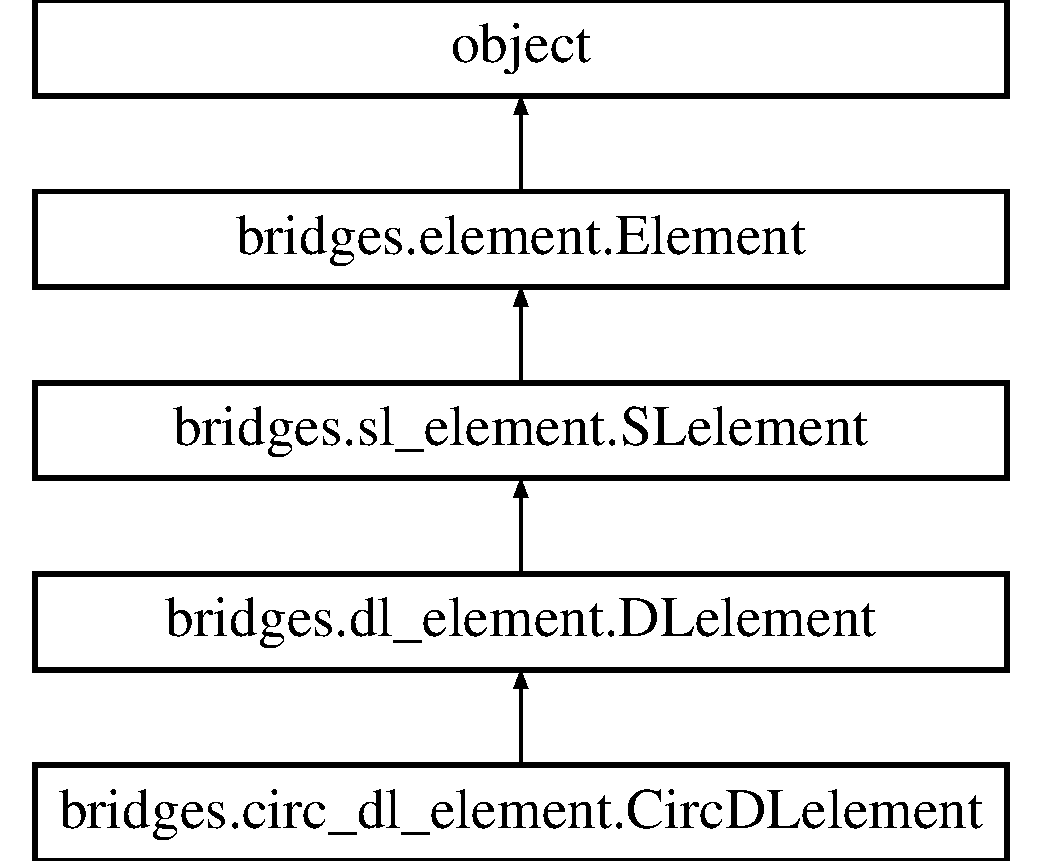
\includegraphics[height=4.000000cm]{classbridges_1_1circ__dl__element_1_1_circ_d_lelement}
\end{center}
\end{figure}


\subsection{Detailed Description}
This class can be used to instantiate Circular Doubly Linked List Elements. 

Structurally they are the same as doubly linked elements except that each node constructed with the next and the previous pointers points to itself.

User\textquotesingle{}s implementation of the circularly linked list needs to ensure that the last node\textquotesingle{}s next pointer points to the first node and the first node\textquotesingle{}s previous pointer points to the last node, as the visualization generation is dependent on this.

Elements have labels (string) that are displayed on the visualization. Elements take an generic object E as a user defined parameter, which can be any native type or object.

Elements contain a visualizer (Element\+Visualizer) object for setting visual attributes (color, shape, opacity, size), necessary for displaying them in a web browser.

Elements also have a Link\+Visualizer object that is used when they are linked to another element, appropriate for setting link attributes, between the element and its previous or next nodes.

\begin{DoxyAuthor}{Author}
Kalpathi Subramanian, Mathhew Mc\+Quaigue
\end{DoxyAuthor}
\begin{DoxyDate}{Date}
7/17/16, 1/16/17 7/23/19
\end{DoxyDate}
Circular doubly linked list tutorial\+: \href{http://bridgesuncc.github.io/tutorials/CircularDoublyLinkedList.html}{\tt http\+://bridgesuncc.\+github.\+io/tutorials/\+Circular\+Doubly\+Linked\+List.\+html} \subsection*{Public Member Functions}
\begin{DoxyCompactItemize}
\item 
def \hyperlink{classbridges_1_1circ__dl__element_1_1_circ_d_lelement_a9536764f84d69deb9f7e03d6802a71b6}{\+\_\+\+\_\+init\+\_\+\+\_\+} (self, kwargs)
\begin{DoxyCompactList}\small\item\em Constructor for an Circularly Doubly Linked Element. \end{DoxyCompactList}\item 
def \hyperlink{classbridges_1_1circ__dl__element_1_1_circ_d_lelement_ac33a5699a662730bb6f292654e6896dc}{get\+\_\+data\+\_\+structure\+\_\+type} (self)
\begin{DoxyCompactList}\small\item\em Gets the data structure type. \end{DoxyCompactList}\item 
def \hyperlink{classbridges_1_1circ__dl__element_1_1_circ_d_lelement_a09b8b12344743709cce1d5fd926b88e9}{next} (self)
\begin{DoxyCompactList}\small\item\em Getter for the next element of this \hyperlink{classbridges_1_1circ__dl__element_1_1_circ_d_lelement}{Circ\+D\+Lelement}. \end{DoxyCompactList}\item 
def \hyperlink{classbridges_1_1circ__dl__element_1_1_circ_d_lelement_a842efa9c0ad878fe34b343600a23d9aa}{next} (self, next)
\begin{DoxyCompactList}\small\item\em Setter for the next element for this \hyperlink{classbridges_1_1circ__dl__element_1_1_circ_d_lelement}{Circ\+D\+Lelement}. \end{DoxyCompactList}\item 
def \hyperlink{classbridges_1_1circ__dl__element_1_1_circ_d_lelement_aa2ebe17f407680a6a4fc886ef9516d61}{prev} (self)
\begin{DoxyCompactList}\small\item\em Getter for the prev element of this \hyperlink{classbridges_1_1circ__dl__element_1_1_circ_d_lelement}{Circ\+D\+Lelement}. \end{DoxyCompactList}\item 
def \hyperlink{classbridges_1_1circ__dl__element_1_1_circ_d_lelement_a5b62548af44a610a2230258fe641d8a2}{prev} (self, prev)
\begin{DoxyCompactList}\small\item\em Setter for the prev element of this \hyperlink{classbridges_1_1circ__dl__element_1_1_circ_d_lelement}{Circ\+D\+Lelement}. \end{DoxyCompactList}\end{DoxyCompactItemize}
\subsection*{Public Attributes}
\begin{DoxyCompactItemize}
\item 
\hyperlink{classbridges_1_1circ__dl__element_1_1_circ_d_lelement_a0f01f7ff433628bac241d7c069a476fa}{next}
\item 
\hyperlink{classbridges_1_1circ__dl__element_1_1_circ_d_lelement_a78ed845303a07e303bcbb39f015843d0}{prev}
\end{DoxyCompactItemize}
\subsection*{Additional Inherited Members}


\subsection{Constructor \& Destructor Documentation}
\mbox{\Hypertarget{classbridges_1_1circ__dl__element_1_1_circ_d_lelement_a9536764f84d69deb9f7e03d6802a71b6}\label{classbridges_1_1circ__dl__element_1_1_circ_d_lelement_a9536764f84d69deb9f7e03d6802a71b6}} 
\index{bridges\+::circ\+\_\+dl\+\_\+element\+::\+Circ\+D\+Lelement@{bridges\+::circ\+\_\+dl\+\_\+element\+::\+Circ\+D\+Lelement}!\+\_\+\+\_\+init\+\_\+\+\_\+@{\+\_\+\+\_\+init\+\_\+\+\_\+}}
\index{\+\_\+\+\_\+init\+\_\+\+\_\+@{\+\_\+\+\_\+init\+\_\+\+\_\+}!bridges\+::circ\+\_\+dl\+\_\+element\+::\+Circ\+D\+Lelement@{bridges\+::circ\+\_\+dl\+\_\+element\+::\+Circ\+D\+Lelement}}
\subsubsection{\texorpdfstring{\+\_\+\+\_\+init\+\_\+\+\_\+()}{\_\_init\_\_()}}
{\footnotesize\ttfamily def bridges.\+circ\+\_\+dl\+\_\+element.\+Circ\+D\+Lelement.\+\_\+\+\_\+init\+\_\+\+\_\+ (\begin{DoxyParamCaption}\item[{}]{self,  }\item[{}]{kwargs,  }\item[{}]{None }\end{DoxyParamCaption})}



Constructor for an Circularly Doubly Linked Element. 


\begin{DoxyParams}{Parameters}
{\em label} & T\+He label for this \hyperlink{classbridges_1_1circ__dl__element_1_1_circ_d_lelement}{Circ\+D\+Lelement} \\
\hline
{\em e} & the generic element object that this \hyperlink{classbridges_1_1circ__dl__element_1_1_circ_d_lelement}{Circ\+D\+Lelement} will hold \\
\hline
{\em next} & the next D\+Lelement that should be assigned to the next pointer \\
\hline
{\em prev} & T\+He previous D\+Lelement that should be assigned to the next pointer \\
\hline
\end{DoxyParams}
\begin{DoxyReturn}{Returns}


None 
\end{DoxyReturn}


\subsection{Member Function Documentation}
\mbox{\Hypertarget{classbridges_1_1circ__dl__element_1_1_circ_d_lelement_ac33a5699a662730bb6f292654e6896dc}\label{classbridges_1_1circ__dl__element_1_1_circ_d_lelement_ac33a5699a662730bb6f292654e6896dc}} 
\index{bridges\+::circ\+\_\+dl\+\_\+element\+::\+Circ\+D\+Lelement@{bridges\+::circ\+\_\+dl\+\_\+element\+::\+Circ\+D\+Lelement}!get\+\_\+data\+\_\+structure\+\_\+type@{get\+\_\+data\+\_\+structure\+\_\+type}}
\index{get\+\_\+data\+\_\+structure\+\_\+type@{get\+\_\+data\+\_\+structure\+\_\+type}!bridges\+::circ\+\_\+dl\+\_\+element\+::\+Circ\+D\+Lelement@{bridges\+::circ\+\_\+dl\+\_\+element\+::\+Circ\+D\+Lelement}}
\subsubsection{\texorpdfstring{get\+\_\+data\+\_\+structure\+\_\+type()}{get\_data\_structure\_type()}}
{\footnotesize\ttfamily def bridges.\+circ\+\_\+dl\+\_\+element.\+Circ\+D\+Lelement.\+get\+\_\+data\+\_\+structure\+\_\+type (\begin{DoxyParamCaption}\item[{}]{self,  }\item[{}]{str }\end{DoxyParamCaption})}



Gets the data structure type. 

\begin{DoxyReturn}{Returns}


None 
\end{DoxyReturn}
\mbox{\Hypertarget{classbridges_1_1circ__dl__element_1_1_circ_d_lelement_a09b8b12344743709cce1d5fd926b88e9}\label{classbridges_1_1circ__dl__element_1_1_circ_d_lelement_a09b8b12344743709cce1d5fd926b88e9}} 
\index{bridges\+::circ\+\_\+dl\+\_\+element\+::\+Circ\+D\+Lelement@{bridges\+::circ\+\_\+dl\+\_\+element\+::\+Circ\+D\+Lelement}!next@{next}}
\index{next@{next}!bridges\+::circ\+\_\+dl\+\_\+element\+::\+Circ\+D\+Lelement@{bridges\+::circ\+\_\+dl\+\_\+element\+::\+Circ\+D\+Lelement}}
\subsubsection{\texorpdfstring{next()}{next()}\hspace{0.1cm}{\footnotesize\ttfamily [1/2]}}
{\footnotesize\ttfamily def bridges.\+circ\+\_\+dl\+\_\+element.\+Circ\+D\+Lelement.\+next (\begin{DoxyParamCaption}\item[{}]{self }\end{DoxyParamCaption})}



Getter for the next element of this \hyperlink{classbridges_1_1circ__dl__element_1_1_circ_d_lelement}{Circ\+D\+Lelement}. 

\begin{DoxyReturn}{Returns}


D\+Lelement the following element 
\end{DoxyReturn}
\mbox{\Hypertarget{classbridges_1_1circ__dl__element_1_1_circ_d_lelement_a842efa9c0ad878fe34b343600a23d9aa}\label{classbridges_1_1circ__dl__element_1_1_circ_d_lelement_a842efa9c0ad878fe34b343600a23d9aa}} 
\index{bridges\+::circ\+\_\+dl\+\_\+element\+::\+Circ\+D\+Lelement@{bridges\+::circ\+\_\+dl\+\_\+element\+::\+Circ\+D\+Lelement}!next@{next}}
\index{next@{next}!bridges\+::circ\+\_\+dl\+\_\+element\+::\+Circ\+D\+Lelement@{bridges\+::circ\+\_\+dl\+\_\+element\+::\+Circ\+D\+Lelement}}
\subsubsection{\texorpdfstring{next()}{next()}\hspace{0.1cm}{\footnotesize\ttfamily [2/2]}}
{\footnotesize\ttfamily def bridges.\+circ\+\_\+dl\+\_\+element.\+Circ\+D\+Lelement.\+next (\begin{DoxyParamCaption}\item[{}]{self,  }\item[{}]{next,  }\item[{}]{None }\end{DoxyParamCaption})}



Setter for the next element for this \hyperlink{classbridges_1_1circ__dl__element_1_1_circ_d_lelement}{Circ\+D\+Lelement}. 

(D\+Lelement) next\+: the next element to be set \begin{DoxyReturn}{Returns}


None 
\end{DoxyReturn}
\mbox{\Hypertarget{classbridges_1_1circ__dl__element_1_1_circ_d_lelement_aa2ebe17f407680a6a4fc886ef9516d61}\label{classbridges_1_1circ__dl__element_1_1_circ_d_lelement_aa2ebe17f407680a6a4fc886ef9516d61}} 
\index{bridges\+::circ\+\_\+dl\+\_\+element\+::\+Circ\+D\+Lelement@{bridges\+::circ\+\_\+dl\+\_\+element\+::\+Circ\+D\+Lelement}!prev@{prev}}
\index{prev@{prev}!bridges\+::circ\+\_\+dl\+\_\+element\+::\+Circ\+D\+Lelement@{bridges\+::circ\+\_\+dl\+\_\+element\+::\+Circ\+D\+Lelement}}
\subsubsection{\texorpdfstring{prev()}{prev()}\hspace{0.1cm}{\footnotesize\ttfamily [1/2]}}
{\footnotesize\ttfamily def bridges.\+circ\+\_\+dl\+\_\+element.\+Circ\+D\+Lelement.\+prev (\begin{DoxyParamCaption}\item[{}]{self }\end{DoxyParamCaption})}



Getter for the prev element of this \hyperlink{classbridges_1_1circ__dl__element_1_1_circ_d_lelement}{Circ\+D\+Lelement}. 

\begin{DoxyReturn}{Returns}


D\+Lelement the prev element in the list 
\end{DoxyReturn}
\mbox{\Hypertarget{classbridges_1_1circ__dl__element_1_1_circ_d_lelement_a5b62548af44a610a2230258fe641d8a2}\label{classbridges_1_1circ__dl__element_1_1_circ_d_lelement_a5b62548af44a610a2230258fe641d8a2}} 
\index{bridges\+::circ\+\_\+dl\+\_\+element\+::\+Circ\+D\+Lelement@{bridges\+::circ\+\_\+dl\+\_\+element\+::\+Circ\+D\+Lelement}!prev@{prev}}
\index{prev@{prev}!bridges\+::circ\+\_\+dl\+\_\+element\+::\+Circ\+D\+Lelement@{bridges\+::circ\+\_\+dl\+\_\+element\+::\+Circ\+D\+Lelement}}
\subsubsection{\texorpdfstring{prev()}{prev()}\hspace{0.1cm}{\footnotesize\ttfamily [2/2]}}
{\footnotesize\ttfamily def bridges.\+circ\+\_\+dl\+\_\+element.\+Circ\+D\+Lelement.\+prev (\begin{DoxyParamCaption}\item[{}]{self,  }\item[{}]{prev,  }\item[{}]{None }\end{DoxyParamCaption})}



Setter for the prev element of this \hyperlink{classbridges_1_1circ__dl__element_1_1_circ_d_lelement}{Circ\+D\+Lelement}. 

(D\+Lelement) prev\+: The prev element to be set \begin{DoxyReturn}{Returns}


None 
\end{DoxyReturn}


\subsection{Member Data Documentation}
\mbox{\Hypertarget{classbridges_1_1circ__dl__element_1_1_circ_d_lelement_a0f01f7ff433628bac241d7c069a476fa}\label{classbridges_1_1circ__dl__element_1_1_circ_d_lelement_a0f01f7ff433628bac241d7c069a476fa}} 
\index{bridges\+::circ\+\_\+dl\+\_\+element\+::\+Circ\+D\+Lelement@{bridges\+::circ\+\_\+dl\+\_\+element\+::\+Circ\+D\+Lelement}!next@{next}}
\index{next@{next}!bridges\+::circ\+\_\+dl\+\_\+element\+::\+Circ\+D\+Lelement@{bridges\+::circ\+\_\+dl\+\_\+element\+::\+Circ\+D\+Lelement}}
\subsubsection{\texorpdfstring{next}{next}}
{\footnotesize\ttfamily bridges.\+circ\+\_\+dl\+\_\+element.\+Circ\+D\+Lelement.\+next}

\mbox{\Hypertarget{classbridges_1_1circ__dl__element_1_1_circ_d_lelement_a78ed845303a07e303bcbb39f015843d0}\label{classbridges_1_1circ__dl__element_1_1_circ_d_lelement_a78ed845303a07e303bcbb39f015843d0}} 
\index{bridges\+::circ\+\_\+dl\+\_\+element\+::\+Circ\+D\+Lelement@{bridges\+::circ\+\_\+dl\+\_\+element\+::\+Circ\+D\+Lelement}!prev@{prev}}
\index{prev@{prev}!bridges\+::circ\+\_\+dl\+\_\+element\+::\+Circ\+D\+Lelement@{bridges\+::circ\+\_\+dl\+\_\+element\+::\+Circ\+D\+Lelement}}
\subsubsection{\texorpdfstring{prev}{prev}}
{\footnotesize\ttfamily bridges.\+circ\+\_\+dl\+\_\+element.\+Circ\+D\+Lelement.\+prev}



The documentation for this class was generated from the following file\+:\begin{DoxyCompactItemize}
\item 
/home/erik/work/bridges/bridges-\/python/bridges/\hyperlink{circ__dl__element_8py}{circ\+\_\+dl\+\_\+element.\+py}\end{DoxyCompactItemize}

\hypertarget{classbridges_1_1circ__sl__element_1_1_circ_s_lelement}{}\section{bridges.\+circ\+\_\+sl\+\_\+element.\+Circ\+S\+Lelement Class Reference}
\label{classbridges_1_1circ__sl__element_1_1_circ_s_lelement}\index{bridges.\+circ\+\_\+sl\+\_\+element.\+Circ\+S\+Lelement@{bridges.\+circ\+\_\+sl\+\_\+element.\+Circ\+S\+Lelement}}
Inheritance diagram for bridges.\+circ\+\_\+sl\+\_\+element.\+Circ\+S\+Lelement\+:\begin{figure}[H]
\begin{center}
\leavevmode
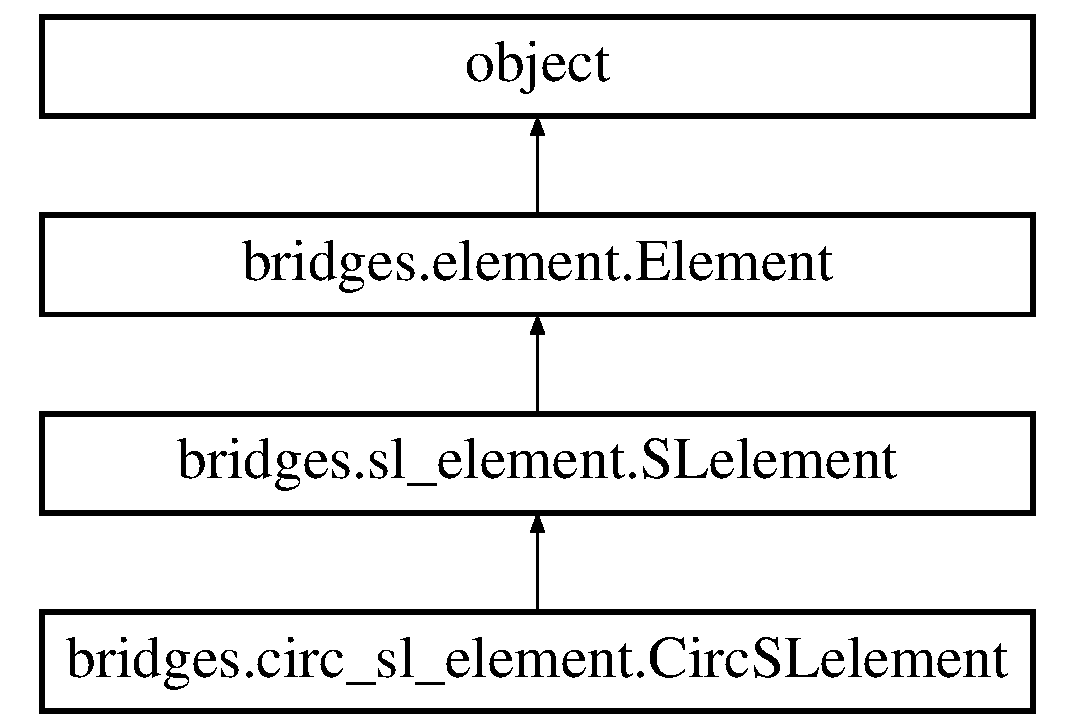
\includegraphics[height=3.000000cm]{classbridges_1_1circ__sl__element_1_1_circ_s_lelement}
\end{center}
\end{figure}


\subsection{Detailed Description}
This class can be used to instantiate Singly Linked Circular List Elements. 

Structurally they are the same as singly linked elements except that each node constructed with the next point pointing to itself; User\textquotesingle{}s implementation of the circularly linked list needs to ensure that the last node points to first node of the list, as the visualization generation is dependent on this.

Elements have labels (string) that are displayed on the visualization. Elements take an generic object as a user defined parameter, E, which can be any native type or object.

Elements contains a visualizer (Element\+Visualizer) object for setting visual attributes (color, shape, opacity, size), necessary for displaying them in a web browser.

Elements also have a Link\+Visualizer object that is used when they are linked to another element, appropriate for setting link attributes, between an element and its next element.

\begin{DoxyAuthor}{Author}
Kalpathi Subramanian, Matthew Mc\+Quaigue
\end{DoxyAuthor}
\begin{DoxyDate}{Date}
6/22/16, 1/7/17, 5/17/17, 7/23/19
\end{DoxyDate}
Circular singly linked list tutorial\+: \href{http://bridgesuncc.github.io/tutorials/CircularSinglyLinkedList.html}{\tt http\+://bridgesuncc.\+github.\+io/tutorials/\+Circular\+Singly\+Linked\+List.\+html} \subsection*{Public Member Functions}
\begin{DoxyCompactItemize}
\item 
def \hyperlink{classbridges_1_1circ__sl__element_1_1_circ_s_lelement_a8ffff39d70e7e94d8d8573e555a6ff35}{\+\_\+\+\_\+init\+\_\+\+\_\+} (self, kwargs)
\begin{DoxyCompactList}\small\item\em The constructor for a Circular Singly Linked Element. \end{DoxyCompactList}\item 
def \hyperlink{classbridges_1_1circ__sl__element_1_1_circ_s_lelement_a82b1dbb8592c943eb68161ee60ac3492}{get\+\_\+data\+\_\+structure\+\_\+type} (self)
\begin{DoxyCompactList}\small\item\em Gets the data structure type. \end{DoxyCompactList}\item 
def \hyperlink{classbridges_1_1circ__sl__element_1_1_circ_s_lelement_a5abc123aa4a20414a02785f3b1cc342a}{next} (self)
\begin{DoxyCompactList}\small\item\em Getter for the next element of this \hyperlink{classbridges_1_1circ__sl__element_1_1_circ_s_lelement}{Circ\+S\+Lelement}. \end{DoxyCompactList}\item 
def \hyperlink{classbridges_1_1circ__sl__element_1_1_circ_s_lelement_a0215303874e167e22f92e4adbdee1e84}{next} (self, n)
\begin{DoxyCompactList}\small\item\em Setter for the next element in Circular list. \end{DoxyCompactList}\end{DoxyCompactItemize}
\subsection*{Public Attributes}
\begin{DoxyCompactItemize}
\item 
\hyperlink{classbridges_1_1circ__sl__element_1_1_circ_s_lelement_afc8fa34bcbc539e7966db5ec471e3959}{next}
\end{DoxyCompactItemize}
\subsection*{Additional Inherited Members}


\subsection{Constructor \& Destructor Documentation}
\mbox{\Hypertarget{classbridges_1_1circ__sl__element_1_1_circ_s_lelement_a8ffff39d70e7e94d8d8573e555a6ff35}\label{classbridges_1_1circ__sl__element_1_1_circ_s_lelement_a8ffff39d70e7e94d8d8573e555a6ff35}} 
\index{bridges\+::circ\+\_\+sl\+\_\+element\+::\+Circ\+S\+Lelement@{bridges\+::circ\+\_\+sl\+\_\+element\+::\+Circ\+S\+Lelement}!\+\_\+\+\_\+init\+\_\+\+\_\+@{\+\_\+\+\_\+init\+\_\+\+\_\+}}
\index{\+\_\+\+\_\+init\+\_\+\+\_\+@{\+\_\+\+\_\+init\+\_\+\+\_\+}!bridges\+::circ\+\_\+sl\+\_\+element\+::\+Circ\+S\+Lelement@{bridges\+::circ\+\_\+sl\+\_\+element\+::\+Circ\+S\+Lelement}}
\subsubsection{\texorpdfstring{\+\_\+\+\_\+init\+\_\+\+\_\+()}{\_\_init\_\_()}}
{\footnotesize\ttfamily def bridges.\+circ\+\_\+sl\+\_\+element.\+Circ\+S\+Lelement.\+\_\+\+\_\+init\+\_\+\+\_\+ (\begin{DoxyParamCaption}\item[{}]{self,  }\item[{}]{kwargs,  }\item[{}]{None }\end{DoxyParamCaption})}



The constructor for a Circular Singly Linked Element. 


\begin{DoxyParams}{Parameters}
{\em e} & the generic object that this \hyperlink{classbridges_1_1circ__sl__element_1_1_circ_s_lelement}{Circ\+S\+Lelement} will hold \\
\hline
{\em label} & The label of this \hyperlink{classbridges_1_1circ__sl__element_1_1_circ_s_lelement}{Circ\+S\+Lelement} \\
\hline
{\em next} & The \hyperlink{classbridges_1_1circ__sl__element_1_1_circ_s_lelement}{Circ\+S\+Lelement} that should be assigned to the next pointer \\
\hline
\end{DoxyParams}
\begin{DoxyReturn}{Returns}


None 
\end{DoxyReturn}


\subsection{Member Function Documentation}
\mbox{\Hypertarget{classbridges_1_1circ__sl__element_1_1_circ_s_lelement_a82b1dbb8592c943eb68161ee60ac3492}\label{classbridges_1_1circ__sl__element_1_1_circ_s_lelement_a82b1dbb8592c943eb68161ee60ac3492}} 
\index{bridges\+::circ\+\_\+sl\+\_\+element\+::\+Circ\+S\+Lelement@{bridges\+::circ\+\_\+sl\+\_\+element\+::\+Circ\+S\+Lelement}!get\+\_\+data\+\_\+structure\+\_\+type@{get\+\_\+data\+\_\+structure\+\_\+type}}
\index{get\+\_\+data\+\_\+structure\+\_\+type@{get\+\_\+data\+\_\+structure\+\_\+type}!bridges\+::circ\+\_\+sl\+\_\+element\+::\+Circ\+S\+Lelement@{bridges\+::circ\+\_\+sl\+\_\+element\+::\+Circ\+S\+Lelement}}
\subsubsection{\texorpdfstring{get\+\_\+data\+\_\+structure\+\_\+type()}{get\_data\_structure\_type()}}
{\footnotesize\ttfamily def bridges.\+circ\+\_\+sl\+\_\+element.\+Circ\+S\+Lelement.\+get\+\_\+data\+\_\+structure\+\_\+type (\begin{DoxyParamCaption}\item[{}]{self,  }\item[{}]{str }\end{DoxyParamCaption})}



Gets the data structure type. 

\begin{DoxyReturn}{Returns}


str representing the data structure type 
\end{DoxyReturn}
\mbox{\Hypertarget{classbridges_1_1circ__sl__element_1_1_circ_s_lelement_a5abc123aa4a20414a02785f3b1cc342a}\label{classbridges_1_1circ__sl__element_1_1_circ_s_lelement_a5abc123aa4a20414a02785f3b1cc342a}} 
\index{bridges\+::circ\+\_\+sl\+\_\+element\+::\+Circ\+S\+Lelement@{bridges\+::circ\+\_\+sl\+\_\+element\+::\+Circ\+S\+Lelement}!next@{next}}
\index{next@{next}!bridges\+::circ\+\_\+sl\+\_\+element\+::\+Circ\+S\+Lelement@{bridges\+::circ\+\_\+sl\+\_\+element\+::\+Circ\+S\+Lelement}}
\subsubsection{\texorpdfstring{next()}{next()}\hspace{0.1cm}{\footnotesize\ttfamily [1/2]}}
{\footnotesize\ttfamily def bridges.\+circ\+\_\+sl\+\_\+element.\+Circ\+S\+Lelement.\+next (\begin{DoxyParamCaption}\item[{}]{self }\end{DoxyParamCaption})}



Getter for the next element of this \hyperlink{classbridges_1_1circ__sl__element_1_1_circ_s_lelement}{Circ\+S\+Lelement}. 

\begin{DoxyReturn}{Returns}


S\+Lelement the element that follows this element 
\end{DoxyReturn}
\mbox{\Hypertarget{classbridges_1_1circ__sl__element_1_1_circ_s_lelement_a0215303874e167e22f92e4adbdee1e84}\label{classbridges_1_1circ__sl__element_1_1_circ_s_lelement_a0215303874e167e22f92e4adbdee1e84}} 
\index{bridges\+::circ\+\_\+sl\+\_\+element\+::\+Circ\+S\+Lelement@{bridges\+::circ\+\_\+sl\+\_\+element\+::\+Circ\+S\+Lelement}!next@{next}}
\index{next@{next}!bridges\+::circ\+\_\+sl\+\_\+element\+::\+Circ\+S\+Lelement@{bridges\+::circ\+\_\+sl\+\_\+element\+::\+Circ\+S\+Lelement}}
\subsubsection{\texorpdfstring{next()}{next()}\hspace{0.1cm}{\footnotesize\ttfamily [2/2]}}
{\footnotesize\ttfamily def bridges.\+circ\+\_\+sl\+\_\+element.\+Circ\+S\+Lelement.\+next (\begin{DoxyParamCaption}\item[{}]{self,  }\item[{}]{n,  }\item[{}]{None }\end{DoxyParamCaption})}



Setter for the next element in Circular list. 


\begin{DoxyParams}{Parameters}
{\em n} & the next element to be set \\
\hline
\end{DoxyParams}
\begin{DoxyReturn}{Returns}

\end{DoxyReturn}
\begin{DoxyParagraph}{None}

\end{DoxyParagraph}


\subsection{Member Data Documentation}
\mbox{\Hypertarget{classbridges_1_1circ__sl__element_1_1_circ_s_lelement_afc8fa34bcbc539e7966db5ec471e3959}\label{classbridges_1_1circ__sl__element_1_1_circ_s_lelement_afc8fa34bcbc539e7966db5ec471e3959}} 
\index{bridges\+::circ\+\_\+sl\+\_\+element\+::\+Circ\+S\+Lelement@{bridges\+::circ\+\_\+sl\+\_\+element\+::\+Circ\+S\+Lelement}!next@{next}}
\index{next@{next}!bridges\+::circ\+\_\+sl\+\_\+element\+::\+Circ\+S\+Lelement@{bridges\+::circ\+\_\+sl\+\_\+element\+::\+Circ\+S\+Lelement}}
\subsubsection{\texorpdfstring{next}{next}}
{\footnotesize\ttfamily bridges.\+circ\+\_\+sl\+\_\+element.\+Circ\+S\+Lelement.\+next}



The documentation for this class was generated from the following file\+:\begin{DoxyCompactItemize}
\item 
/home/erik/work/bridges/bridges-\/python/bridges/\hyperlink{circ__sl__element_8py}{circ\+\_\+sl\+\_\+element.\+py}\end{DoxyCompactItemize}

\hypertarget{classbridges_1_1color_1_1_color}{}\section{bridges.\+color.\+Color Class Reference}
\label{classbridges_1_1color_1_1_color}\index{bridges.\+color.\+Color@{bridges.\+color.\+Color}}
Inheritance diagram for bridges.\+color.\+Color\+:\begin{figure}[H]
\begin{center}
\leavevmode
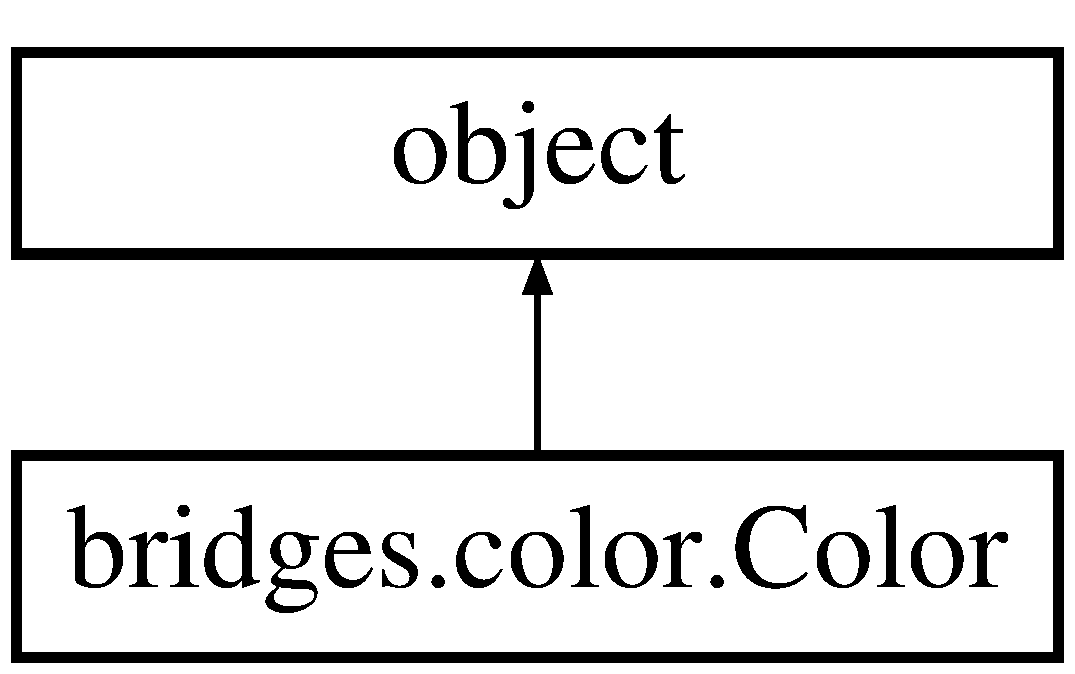
\includegraphics[height=2.000000cm]{classbridges_1_1color_1_1_color}
\end{center}
\end{figure}
\subsection*{Public Member Functions}
\begin{DoxyCompactItemize}
\item 
def \mbox{\hyperlink{classbridges_1_1color_1_1_color_ab2b29fe67b6ad8dddde7ff8eddedcce0}{red}} (self)
\item 
def \mbox{\hyperlink{classbridges_1_1color_1_1_color_a39719b281c9095293a1445c6deb7792b}{red}}
\item 
def \mbox{\hyperlink{classbridges_1_1color_1_1_color_ab2b29fe67b6ad8dddde7ff8eddedcce0}{red}} (self)
\item 
def \mbox{\hyperlink{classbridges_1_1color_1_1_color_a86ec858a55491936054abcea865498ec}{green}} (self)
\item 
def \mbox{\hyperlink{classbridges_1_1color_1_1_color_a4c0826514c64b53910270336d357ad80}{green}}
\item 
def \mbox{\hyperlink{classbridges_1_1color_1_1_color_a86ec858a55491936054abcea865498ec}{green}} (self)
\item 
def \mbox{\hyperlink{classbridges_1_1color_1_1_color_a14f94eb29dcabf578a1932c5477e12f3}{blue}} (self)
\item 
def \mbox{\hyperlink{classbridges_1_1color_1_1_color_a0673063270c8a522b086a916f09dd1f5}{blue}}
\item 
def \mbox{\hyperlink{classbridges_1_1color_1_1_color_a14f94eb29dcabf578a1932c5477e12f3}{blue}} (self)
\item 
def \mbox{\hyperlink{classbridges_1_1color_1_1_color_ae5dc631fcda27156867b21109620ae21}{alpha}} (self)
\item 
def \mbox{\hyperlink{classbridges_1_1color_1_1_color_ab57c1e881ebb14bccefb870a9fa2ac1d}{alpha}}
\item 
def \mbox{\hyperlink{classbridges_1_1color_1_1_color_ae5dc631fcda27156867b21109620ae21}{alpha}} (self)
\item 
def \mbox{\hyperlink{classbridges_1_1color_1_1_color_a7653dfb80aa5ec25ed14314ffa79d1f2}{rgba}} (self, int, int, int, float)
\item 
def \mbox{\hyperlink{classbridges_1_1color_1_1_color_aa3d8dcfea52715f28400b08bf15e94ab}{rgba}}
\item 
def \mbox{\hyperlink{classbridges_1_1color_1_1_color_a23f98340da1b581d67592e18317d08bc}{rgba}} (self)
\item 
def \mbox{\hyperlink{classbridges_1_1color_1_1_color_aacbbede0aceb8f1ca36d78379614bb1a}{\+\_\+\+\_\+init\+\_\+\+\_\+}} (self, args, kwargs)
\item 
def \mbox{\hyperlink{classbridges_1_1color_1_1_color_a99b17a81feb1737f8b29c93ae9ef4bc8}{set\+\_\+color}} (self, args, kwargs)
\item 
def \mbox{\hyperlink{classbridges_1_1color_1_1_color_a9b5c8db77c60c49dabf55aa634930704}{set\+\_\+red}}
\item 
def \mbox{\hyperlink{classbridges_1_1color_1_1_color_a492cd26c235ab042ae01a6144c22a6c5}{get\+\_\+red}} (self)
\item 
def \mbox{\hyperlink{classbridges_1_1color_1_1_color_a321743b2baebea451a7fc1428414545e}{set\+\_\+green}}
\item 
def \mbox{\hyperlink{classbridges_1_1color_1_1_color_a6622d2dd9e8cb460a99ae1d918d74e90}{get\+\_\+green}} (self)
\item 
def \mbox{\hyperlink{classbridges_1_1color_1_1_color_a76943ac7fe2c8becae24e338b48d21af}{set\+\_\+blue}}
\item 
def \mbox{\hyperlink{classbridges_1_1color_1_1_color_a250ecbab8a89b5e46d7bd0b258ef6bf2}{get\+\_\+blue}} (self)
\item 
def \mbox{\hyperlink{classbridges_1_1color_1_1_color_a305a0aa465be51fcdd1c77461c76c7e1}{set\+\_\+alpha}}
\item 
def \mbox{\hyperlink{classbridges_1_1color_1_1_color_afbf82e4cde5b45ff48371aadd023a777}{get\+\_\+alpha}} (self)
\item 
def \mbox{\hyperlink{classbridges_1_1color_1_1_color_a30bc8e2023395c584eb256972abc7c1b}{get\+\_\+byte\+\_\+representation}} (self)
\item 
def \mbox{\hyperlink{classbridges_1_1color_1_1_color_ae5677a0858252f0b33da13866fb62786}{\+\_\+\+\_\+eq\+\_\+\+\_\+}} (self, other)
\end{DoxyCompactItemize}
\subsection*{Public Attributes}
\begin{DoxyCompactItemize}
\item 
\mbox{\hyperlink{classbridges_1_1color_1_1_color_a2e170f068eeb77ace0427d23b36f2b27}{alpha}}
\item 
\mbox{\hyperlink{classbridges_1_1color_1_1_color_abb0aa417808af0140d3448a2e49d2d15}{red}}
\item 
\mbox{\hyperlink{classbridges_1_1color_1_1_color_a6f14b2d3ec82052c1aeb259ee687059d}{green}}
\item 
\mbox{\hyperlink{classbridges_1_1color_1_1_color_a2c5081c47a43419bb1c5dbbd9c72a21e}{blue}}
\end{DoxyCompactItemize}


\subsection{Detailed Description}
\begin{DoxyVerb}This class is used to represent colors in bridges.

We use and RGBA model to represent colors, with the Red Green and Blue components ranging from 0-255,
with the alpha ranging from 0.0-1.0 inclusive.

We use webcolors to handle color names passed to the constructor/set_color function.
https://webcolors.readthedocs.io/en/1.8.1/
All CSS3 color names should be valid:
https://developer.mozilla.org/en-US/docs/Web/CSS/color_value
https://www.w3.org/TR/css-color-3/#svg-color

Attributes:
    red (int): red component of color ranging from 0-255 inclusive (default 0)
    green (int): green component of color ranging from 0-255 inclusive (default 0)
    blue (int): blue component of color ranging from 0-255 inclusive (default 0)
    alpha (float): alpha component of color ranging from 0.0-1.0 inclusive (default 1.0)
    rgba (tuple(int, int, int, alpha)): RGBA components as respective tuple
Args:
    args: int, int, int, Optional(float) or a str as singular arg
    kwargs:
        r or red: Optional(int)
        b or blue: Optional(int)
        g or green: Optional(int)
        a or alpha: Optional(float)
        col_name: Optional(str)
Raises:
    ValueError: if args is not 3 ints with an optional 4th arg for alpha or just one str arg
    ValueError: if a str passed is not a valid webcolor
    ValueError: if any of the RGBA values are outside of their respective range
Examples:
    >>> my_color = Color("red")
    >>> my_color.rgba
    (255, 0, 0, 1.0)
    >>> my_color = Color(r=255)
    >>> my_color.rgba
    (255, 0, 0, 1.0)
    >>> my_color = Color(255, 0, 0)
    >>> my_color.rgba
    (255, 0, 0, 1.0)
    >>> my_color = Color()
    >>> my_color.red = 255
    >>> my_color.rgba
    (255, 0, 0, 1.0)
\end{DoxyVerb}
 

\subsection{Constructor \& Destructor Documentation}
\mbox{\Hypertarget{classbridges_1_1color_1_1_color_aacbbede0aceb8f1ca36d78379614bb1a}\label{classbridges_1_1color_1_1_color_aacbbede0aceb8f1ca36d78379614bb1a}} 
\index{bridges\+::color\+::\+Color@{bridges\+::color\+::\+Color}!\+\_\+\+\_\+init\+\_\+\+\_\+@{\+\_\+\+\_\+init\+\_\+\+\_\+}}
\index{\+\_\+\+\_\+init\+\_\+\+\_\+@{\+\_\+\+\_\+init\+\_\+\+\_\+}!bridges\+::color\+::\+Color@{bridges\+::color\+::\+Color}}
\subsubsection{\texorpdfstring{\+\_\+\+\_\+init\+\_\+\+\_\+()}{\_\_init\_\_()}}
{\footnotesize\ttfamily def bridges.\+color.\+Color.\+\_\+\+\_\+init\+\_\+\+\_\+ (\begin{DoxyParamCaption}\item[{}]{self,  }\item[{}]{args,  }\item[{}]{kwargs }\end{DoxyParamCaption})}

\begin{DoxyVerb}Constructor for a Color object
Usage: requires either 3 ints 0-255 for RGB and an optional float 0.0-1.0 for alpha or a str of a web color
can also key the RGBA values with r, g, b, a or red, green, blue, alpha respectively and col_name for the str
:param args: int, int, int, optional float or just a str
:param kwargs: r/red: int, b/blue: int, g/green: int optional a/alpha: float or col_name: str
:return: None
\end{DoxyVerb}
 

\subsection{Member Function Documentation}
\mbox{\Hypertarget{classbridges_1_1color_1_1_color_ae5677a0858252f0b33da13866fb62786}\label{classbridges_1_1color_1_1_color_ae5677a0858252f0b33da13866fb62786}} 
\index{bridges\+::color\+::\+Color@{bridges\+::color\+::\+Color}!\+\_\+\+\_\+eq\+\_\+\+\_\+@{\+\_\+\+\_\+eq\+\_\+\+\_\+}}
\index{\+\_\+\+\_\+eq\+\_\+\+\_\+@{\+\_\+\+\_\+eq\+\_\+\+\_\+}!bridges\+::color\+::\+Color@{bridges\+::color\+::\+Color}}
\subsubsection{\texorpdfstring{\+\_\+\+\_\+eq\+\_\+\+\_\+()}{\_\_eq\_\_()}}
{\footnotesize\ttfamily def bridges.\+color.\+Color.\+\_\+\+\_\+eq\+\_\+\+\_\+ (\begin{DoxyParamCaption}\item[{}]{self,  }\item[{}]{other }\end{DoxyParamCaption})}

\begin{DoxyVerb}deep equality check, by value of each RGBA value\end{DoxyVerb}
 \mbox{\Hypertarget{classbridges_1_1color_1_1_color_ae5dc631fcda27156867b21109620ae21}\label{classbridges_1_1color_1_1_color_ae5dc631fcda27156867b21109620ae21}} 
\index{bridges\+::color\+::\+Color@{bridges\+::color\+::\+Color}!alpha@{alpha}}
\index{alpha@{alpha}!bridges\+::color\+::\+Color@{bridges\+::color\+::\+Color}}
\subsubsection{\texorpdfstring{alpha()}{alpha()}\hspace{0.1cm}{\footnotesize\ttfamily [1/3]}}
{\footnotesize\ttfamily def bridges.\+color.\+Color.\+alpha (\begin{DoxyParamCaption}\item[{}]{self,  }\item[{}]{float }\end{DoxyParamCaption})}

\begin{DoxyVerb}alpha component of color
:return float: alpha component of color
Must be a value between 0.0-1.0 inclusive
\end{DoxyVerb}
 \mbox{\Hypertarget{classbridges_1_1color_1_1_color_ab57c1e881ebb14bccefb870a9fa2ac1d}\label{classbridges_1_1color_1_1_color_ab57c1e881ebb14bccefb870a9fa2ac1d}} 
\index{bridges\+::color\+::\+Color@{bridges\+::color\+::\+Color}!alpha@{alpha}}
\index{alpha@{alpha}!bridges\+::color\+::\+Color@{bridges\+::color\+::\+Color}}
\subsubsection{\texorpdfstring{alpha()}{alpha()}\hspace{0.1cm}{\footnotesize\ttfamily [2/3]}}
{\footnotesize\ttfamily def bridges.\+color.\+Color.\+alpha (\begin{DoxyParamCaption}\item[{}]{self,  }\item[{}]{value }\end{DoxyParamCaption})}

\mbox{\Hypertarget{classbridges_1_1color_1_1_color_ae5dc631fcda27156867b21109620ae21}\label{classbridges_1_1color_1_1_color_ae5dc631fcda27156867b21109620ae21}} 
\index{bridges\+::color\+::\+Color@{bridges\+::color\+::\+Color}!alpha@{alpha}}
\index{alpha@{alpha}!bridges\+::color\+::\+Color@{bridges\+::color\+::\+Color}}
\subsubsection{\texorpdfstring{alpha()}{alpha()}\hspace{0.1cm}{\footnotesize\ttfamily [3/3]}}
{\footnotesize\ttfamily def bridges.\+color.\+Color.\+alpha (\begin{DoxyParamCaption}\item[{}]{self }\end{DoxyParamCaption})}

\mbox{\Hypertarget{classbridges_1_1color_1_1_color_a14f94eb29dcabf578a1932c5477e12f3}\label{classbridges_1_1color_1_1_color_a14f94eb29dcabf578a1932c5477e12f3}} 
\index{bridges\+::color\+::\+Color@{bridges\+::color\+::\+Color}!blue@{blue}}
\index{blue@{blue}!bridges\+::color\+::\+Color@{bridges\+::color\+::\+Color}}
\subsubsection{\texorpdfstring{blue()}{blue()}\hspace{0.1cm}{\footnotesize\ttfamily [1/3]}}
{\footnotesize\ttfamily def bridges.\+color.\+Color.\+blue (\begin{DoxyParamCaption}\item[{}]{self,  }\item[{}]{int }\end{DoxyParamCaption})}

\begin{DoxyVerb}blue component of color
:return int: blue component of color
Must be a value between 0-255 inclusive
\end{DoxyVerb}
 \mbox{\Hypertarget{classbridges_1_1color_1_1_color_a0673063270c8a522b086a916f09dd1f5}\label{classbridges_1_1color_1_1_color_a0673063270c8a522b086a916f09dd1f5}} 
\index{bridges\+::color\+::\+Color@{bridges\+::color\+::\+Color}!blue@{blue}}
\index{blue@{blue}!bridges\+::color\+::\+Color@{bridges\+::color\+::\+Color}}
\subsubsection{\texorpdfstring{blue()}{blue()}\hspace{0.1cm}{\footnotesize\ttfamily [2/3]}}
{\footnotesize\ttfamily def bridges.\+color.\+Color.\+blue (\begin{DoxyParamCaption}\item[{}]{self,  }\item[{}]{value }\end{DoxyParamCaption})}

\mbox{\Hypertarget{classbridges_1_1color_1_1_color_a14f94eb29dcabf578a1932c5477e12f3}\label{classbridges_1_1color_1_1_color_a14f94eb29dcabf578a1932c5477e12f3}} 
\index{bridges\+::color\+::\+Color@{bridges\+::color\+::\+Color}!blue@{blue}}
\index{blue@{blue}!bridges\+::color\+::\+Color@{bridges\+::color\+::\+Color}}
\subsubsection{\texorpdfstring{blue()}{blue()}\hspace{0.1cm}{\footnotesize\ttfamily [3/3]}}
{\footnotesize\ttfamily def bridges.\+color.\+Color.\+blue (\begin{DoxyParamCaption}\item[{}]{self }\end{DoxyParamCaption})}

\mbox{\Hypertarget{classbridges_1_1color_1_1_color_afbf82e4cde5b45ff48371aadd023a777}\label{classbridges_1_1color_1_1_color_afbf82e4cde5b45ff48371aadd023a777}} 
\index{bridges\+::color\+::\+Color@{bridges\+::color\+::\+Color}!get\+\_\+alpha@{get\+\_\+alpha}}
\index{get\+\_\+alpha@{get\+\_\+alpha}!bridges\+::color\+::\+Color@{bridges\+::color\+::\+Color}}
\subsubsection{\texorpdfstring{get\+\_\+alpha()}{get\_alpha()}}
{\footnotesize\ttfamily def bridges.\+color.\+Color.\+get\+\_\+alpha (\begin{DoxyParamCaption}\item[{}]{self,  }\item[{}]{float }\end{DoxyParamCaption})}

\begin{DoxyVerb}:return float: alpha component of color\end{DoxyVerb}
 \mbox{\Hypertarget{classbridges_1_1color_1_1_color_a250ecbab8a89b5e46d7bd0b258ef6bf2}\label{classbridges_1_1color_1_1_color_a250ecbab8a89b5e46d7bd0b258ef6bf2}} 
\index{bridges\+::color\+::\+Color@{bridges\+::color\+::\+Color}!get\+\_\+blue@{get\+\_\+blue}}
\index{get\+\_\+blue@{get\+\_\+blue}!bridges\+::color\+::\+Color@{bridges\+::color\+::\+Color}}
\subsubsection{\texorpdfstring{get\+\_\+blue()}{get\_blue()}}
{\footnotesize\ttfamily def bridges.\+color.\+Color.\+get\+\_\+blue (\begin{DoxyParamCaption}\item[{}]{self,  }\item[{}]{int }\end{DoxyParamCaption})}

\begin{DoxyVerb}":return int: blue component of color\end{DoxyVerb}
 \mbox{\Hypertarget{classbridges_1_1color_1_1_color_a30bc8e2023395c584eb256972abc7c1b}\label{classbridges_1_1color_1_1_color_a30bc8e2023395c584eb256972abc7c1b}} 
\index{bridges\+::color\+::\+Color@{bridges\+::color\+::\+Color}!get\+\_\+byte\+\_\+representation@{get\+\_\+byte\+\_\+representation}}
\index{get\+\_\+byte\+\_\+representation@{get\+\_\+byte\+\_\+representation}!bridges\+::color\+::\+Color@{bridges\+::color\+::\+Color}}
\subsubsection{\texorpdfstring{get\+\_\+byte\+\_\+representation()}{get\_byte\_representation()}}
{\footnotesize\ttfamily def bridges.\+color.\+Color.\+get\+\_\+byte\+\_\+representation (\begin{DoxyParamCaption}\item[{}]{self,  }\item[{}]{list }\end{DoxyParamCaption})}

\begin{DoxyVerb}:return list(int):RGBA values as list of ints from 0-255\end{DoxyVerb}
 \mbox{\Hypertarget{classbridges_1_1color_1_1_color_a6622d2dd9e8cb460a99ae1d918d74e90}\label{classbridges_1_1color_1_1_color_a6622d2dd9e8cb460a99ae1d918d74e90}} 
\index{bridges\+::color\+::\+Color@{bridges\+::color\+::\+Color}!get\+\_\+green@{get\+\_\+green}}
\index{get\+\_\+green@{get\+\_\+green}!bridges\+::color\+::\+Color@{bridges\+::color\+::\+Color}}
\subsubsection{\texorpdfstring{get\+\_\+green()}{get\_green()}}
{\footnotesize\ttfamily def bridges.\+color.\+Color.\+get\+\_\+green (\begin{DoxyParamCaption}\item[{}]{self,  }\item[{}]{int }\end{DoxyParamCaption})}

\begin{DoxyVerb}:return int: green component of color\end{DoxyVerb}
 \mbox{\Hypertarget{classbridges_1_1color_1_1_color_a492cd26c235ab042ae01a6144c22a6c5}\label{classbridges_1_1color_1_1_color_a492cd26c235ab042ae01a6144c22a6c5}} 
\index{bridges\+::color\+::\+Color@{bridges\+::color\+::\+Color}!get\+\_\+red@{get\+\_\+red}}
\index{get\+\_\+red@{get\+\_\+red}!bridges\+::color\+::\+Color@{bridges\+::color\+::\+Color}}
\subsubsection{\texorpdfstring{get\+\_\+red()}{get\_red()}}
{\footnotesize\ttfamily def bridges.\+color.\+Color.\+get\+\_\+red (\begin{DoxyParamCaption}\item[{}]{self,  }\item[{}]{int }\end{DoxyParamCaption})}

\begin{DoxyVerb}:return int: red component of color\end{DoxyVerb}
 \mbox{\Hypertarget{classbridges_1_1color_1_1_color_a86ec858a55491936054abcea865498ec}\label{classbridges_1_1color_1_1_color_a86ec858a55491936054abcea865498ec}} 
\index{bridges\+::color\+::\+Color@{bridges\+::color\+::\+Color}!green@{green}}
\index{green@{green}!bridges\+::color\+::\+Color@{bridges\+::color\+::\+Color}}
\subsubsection{\texorpdfstring{green()}{green()}\hspace{0.1cm}{\footnotesize\ttfamily [1/3]}}
{\footnotesize\ttfamily def bridges.\+color.\+Color.\+green (\begin{DoxyParamCaption}\item[{}]{self,  }\item[{}]{int }\end{DoxyParamCaption})}

\begin{DoxyVerb}green component of color
:return int: green component of color
Must be a value between 0-255 inclusive
\end{DoxyVerb}
 \mbox{\Hypertarget{classbridges_1_1color_1_1_color_a4c0826514c64b53910270336d357ad80}\label{classbridges_1_1color_1_1_color_a4c0826514c64b53910270336d357ad80}} 
\index{bridges\+::color\+::\+Color@{bridges\+::color\+::\+Color}!green@{green}}
\index{green@{green}!bridges\+::color\+::\+Color@{bridges\+::color\+::\+Color}}
\subsubsection{\texorpdfstring{green()}{green()}\hspace{0.1cm}{\footnotesize\ttfamily [2/3]}}
{\footnotesize\ttfamily def bridges.\+color.\+Color.\+green (\begin{DoxyParamCaption}\item[{}]{self,  }\item[{}]{value }\end{DoxyParamCaption})}

\mbox{\Hypertarget{classbridges_1_1color_1_1_color_a86ec858a55491936054abcea865498ec}\label{classbridges_1_1color_1_1_color_a86ec858a55491936054abcea865498ec}} 
\index{bridges\+::color\+::\+Color@{bridges\+::color\+::\+Color}!green@{green}}
\index{green@{green}!bridges\+::color\+::\+Color@{bridges\+::color\+::\+Color}}
\subsubsection{\texorpdfstring{green()}{green()}\hspace{0.1cm}{\footnotesize\ttfamily [3/3]}}
{\footnotesize\ttfamily def bridges.\+color.\+Color.\+green (\begin{DoxyParamCaption}\item[{}]{self }\end{DoxyParamCaption})}

\mbox{\Hypertarget{classbridges_1_1color_1_1_color_ab2b29fe67b6ad8dddde7ff8eddedcce0}\label{classbridges_1_1color_1_1_color_ab2b29fe67b6ad8dddde7ff8eddedcce0}} 
\index{bridges\+::color\+::\+Color@{bridges\+::color\+::\+Color}!red@{red}}
\index{red@{red}!bridges\+::color\+::\+Color@{bridges\+::color\+::\+Color}}
\subsubsection{\texorpdfstring{red()}{red()}\hspace{0.1cm}{\footnotesize\ttfamily [1/3]}}
{\footnotesize\ttfamily def bridges.\+color.\+Color.\+red (\begin{DoxyParamCaption}\item[{}]{self,  }\item[{}]{int }\end{DoxyParamCaption})}

\begin{DoxyVerb}red component of color
:return int: red component of color
Must be a value between 0-255 inclusive
\end{DoxyVerb}
 \mbox{\Hypertarget{classbridges_1_1color_1_1_color_a39719b281c9095293a1445c6deb7792b}\label{classbridges_1_1color_1_1_color_a39719b281c9095293a1445c6deb7792b}} 
\index{bridges\+::color\+::\+Color@{bridges\+::color\+::\+Color}!red@{red}}
\index{red@{red}!bridges\+::color\+::\+Color@{bridges\+::color\+::\+Color}}
\subsubsection{\texorpdfstring{red()}{red()}\hspace{0.1cm}{\footnotesize\ttfamily [2/3]}}
{\footnotesize\ttfamily def bridges.\+color.\+Color.\+red (\begin{DoxyParamCaption}\item[{}]{self,  }\item[{}]{value }\end{DoxyParamCaption})}

\mbox{\Hypertarget{classbridges_1_1color_1_1_color_ab2b29fe67b6ad8dddde7ff8eddedcce0}\label{classbridges_1_1color_1_1_color_ab2b29fe67b6ad8dddde7ff8eddedcce0}} 
\index{bridges\+::color\+::\+Color@{bridges\+::color\+::\+Color}!red@{red}}
\index{red@{red}!bridges\+::color\+::\+Color@{bridges\+::color\+::\+Color}}
\subsubsection{\texorpdfstring{red()}{red()}\hspace{0.1cm}{\footnotesize\ttfamily [3/3]}}
{\footnotesize\ttfamily def bridges.\+color.\+Color.\+red (\begin{DoxyParamCaption}\item[{}]{self }\end{DoxyParamCaption})}

\mbox{\Hypertarget{classbridges_1_1color_1_1_color_a7653dfb80aa5ec25ed14314ffa79d1f2}\label{classbridges_1_1color_1_1_color_a7653dfb80aa5ec25ed14314ffa79d1f2}} 
\index{bridges\+::color\+::\+Color@{bridges\+::color\+::\+Color}!rgba@{rgba}}
\index{rgba@{rgba}!bridges\+::color\+::\+Color@{bridges\+::color\+::\+Color}}
\subsubsection{\texorpdfstring{rgba()}{rgba()}\hspace{0.1cm}{\footnotesize\ttfamily [1/3]}}
{\footnotesize\ttfamily def bridges.\+color.\+Color.\+rgba (\begin{DoxyParamCaption}\item[{}]{self,  }\item[{}]{int,  }\item[{}]{int,  }\item[{}]{int,  }\item[{}]{float }\end{DoxyParamCaption})}

\begin{DoxyVerb}RGBA components as respective tuple
Represents the RGBA values of the color as a tuple, can be used to set or get all values at once
:return (int, int, int, float): RGBA values respectively
\end{DoxyVerb}
 \mbox{\Hypertarget{classbridges_1_1color_1_1_color_aa3d8dcfea52715f28400b08bf15e94ab}\label{classbridges_1_1color_1_1_color_aa3d8dcfea52715f28400b08bf15e94ab}} 
\index{bridges\+::color\+::\+Color@{bridges\+::color\+::\+Color}!rgba@{rgba}}
\index{rgba@{rgba}!bridges\+::color\+::\+Color@{bridges\+::color\+::\+Color}}
\subsubsection{\texorpdfstring{rgba()}{rgba()}\hspace{0.1cm}{\footnotesize\ttfamily [2/3]}}
{\footnotesize\ttfamily def bridges.\+color.\+Color.\+rgba (\begin{DoxyParamCaption}\item[{}]{self,  }\item[{}]{rgba }\end{DoxyParamCaption})}

\mbox{\Hypertarget{classbridges_1_1color_1_1_color_a23f98340da1b581d67592e18317d08bc}\label{classbridges_1_1color_1_1_color_a23f98340da1b581d67592e18317d08bc}} 
\index{bridges\+::color\+::\+Color@{bridges\+::color\+::\+Color}!rgba@{rgba}}
\index{rgba@{rgba}!bridges\+::color\+::\+Color@{bridges\+::color\+::\+Color}}
\subsubsection{\texorpdfstring{rgba()}{rgba()}\hspace{0.1cm}{\footnotesize\ttfamily [3/3]}}
{\footnotesize\ttfamily def bridges.\+color.\+Color.\+rgba (\begin{DoxyParamCaption}\item[{}]{self }\end{DoxyParamCaption})}

\mbox{\Hypertarget{classbridges_1_1color_1_1_color_a305a0aa465be51fcdd1c77461c76c7e1}\label{classbridges_1_1color_1_1_color_a305a0aa465be51fcdd1c77461c76c7e1}} 
\index{bridges\+::color\+::\+Color@{bridges\+::color\+::\+Color}!set\+\_\+alpha@{set\+\_\+alpha}}
\index{set\+\_\+alpha@{set\+\_\+alpha}!bridges\+::color\+::\+Color@{bridges\+::color\+::\+Color}}
\subsubsection{\texorpdfstring{set\+\_\+alpha()}{set\_alpha()}}
{\footnotesize\ttfamily def bridges.\+color.\+Color.\+set\+\_\+alpha (\begin{DoxyParamCaption}\item[{}]{self,  }\item[{}]{a }\end{DoxyParamCaption})}

\mbox{\Hypertarget{classbridges_1_1color_1_1_color_a76943ac7fe2c8becae24e338b48d21af}\label{classbridges_1_1color_1_1_color_a76943ac7fe2c8becae24e338b48d21af}} 
\index{bridges\+::color\+::\+Color@{bridges\+::color\+::\+Color}!set\+\_\+blue@{set\+\_\+blue}}
\index{set\+\_\+blue@{set\+\_\+blue}!bridges\+::color\+::\+Color@{bridges\+::color\+::\+Color}}
\subsubsection{\texorpdfstring{set\+\_\+blue()}{set\_blue()}}
{\footnotesize\ttfamily def bridges.\+color.\+Color.\+set\+\_\+blue (\begin{DoxyParamCaption}\item[{}]{self,  }\item[{}]{b }\end{DoxyParamCaption})}

\mbox{\Hypertarget{classbridges_1_1color_1_1_color_a99b17a81feb1737f8b29c93ae9ef4bc8}\label{classbridges_1_1color_1_1_color_a99b17a81feb1737f8b29c93ae9ef4bc8}} 
\index{bridges\+::color\+::\+Color@{bridges\+::color\+::\+Color}!set\+\_\+color@{set\+\_\+color}}
\index{set\+\_\+color@{set\+\_\+color}!bridges\+::color\+::\+Color@{bridges\+::color\+::\+Color}}
\subsubsection{\texorpdfstring{set\+\_\+color()}{set\_color()}}
{\footnotesize\ttfamily def bridges.\+color.\+Color.\+set\+\_\+color (\begin{DoxyParamCaption}\item[{}]{self,  }\item[{}]{args,  }\item[{}]{kwargs,  }\item[{}]{None }\end{DoxyParamCaption})}

\begin{DoxyVerb}Usage: requires either 3 ints 0-255 for RGB and an optional float 0.0-1.0 for alpha or a str of a web color
can also key the RGBA values with r, g, b, a or red, green, blue, alpha respectively and col_name for the str
:param args: int, int, int optional float or str
:param kwargs: r/red: int, b/blue: int, g/green: int optional a/alpha: float or col_name: str
:return: None
\end{DoxyVerb}
 \mbox{\Hypertarget{classbridges_1_1color_1_1_color_a321743b2baebea451a7fc1428414545e}\label{classbridges_1_1color_1_1_color_a321743b2baebea451a7fc1428414545e}} 
\index{bridges\+::color\+::\+Color@{bridges\+::color\+::\+Color}!set\+\_\+green@{set\+\_\+green}}
\index{set\+\_\+green@{set\+\_\+green}!bridges\+::color\+::\+Color@{bridges\+::color\+::\+Color}}
\subsubsection{\texorpdfstring{set\+\_\+green()}{set\_green()}}
{\footnotesize\ttfamily def bridges.\+color.\+Color.\+set\+\_\+green (\begin{DoxyParamCaption}\item[{}]{self,  }\item[{}]{g }\end{DoxyParamCaption})}

\mbox{\Hypertarget{classbridges_1_1color_1_1_color_a9b5c8db77c60c49dabf55aa634930704}\label{classbridges_1_1color_1_1_color_a9b5c8db77c60c49dabf55aa634930704}} 
\index{bridges\+::color\+::\+Color@{bridges\+::color\+::\+Color}!set\+\_\+red@{set\+\_\+red}}
\index{set\+\_\+red@{set\+\_\+red}!bridges\+::color\+::\+Color@{bridges\+::color\+::\+Color}}
\subsubsection{\texorpdfstring{set\+\_\+red()}{set\_red()}}
{\footnotesize\ttfamily def bridges.\+color.\+Color.\+set\+\_\+red (\begin{DoxyParamCaption}\item[{}]{self,  }\item[{}]{r }\end{DoxyParamCaption})}



\subsection{Member Data Documentation}
\mbox{\Hypertarget{classbridges_1_1color_1_1_color_a2e170f068eeb77ace0427d23b36f2b27}\label{classbridges_1_1color_1_1_color_a2e170f068eeb77ace0427d23b36f2b27}} 
\index{bridges\+::color\+::\+Color@{bridges\+::color\+::\+Color}!alpha@{alpha}}
\index{alpha@{alpha}!bridges\+::color\+::\+Color@{bridges\+::color\+::\+Color}}
\subsubsection{\texorpdfstring{alpha}{alpha}}
{\footnotesize\ttfamily bridges.\+color.\+Color.\+alpha}

\mbox{\Hypertarget{classbridges_1_1color_1_1_color_a2c5081c47a43419bb1c5dbbd9c72a21e}\label{classbridges_1_1color_1_1_color_a2c5081c47a43419bb1c5dbbd9c72a21e}} 
\index{bridges\+::color\+::\+Color@{bridges\+::color\+::\+Color}!blue@{blue}}
\index{blue@{blue}!bridges\+::color\+::\+Color@{bridges\+::color\+::\+Color}}
\subsubsection{\texorpdfstring{blue}{blue}}
{\footnotesize\ttfamily bridges.\+color.\+Color.\+blue}

\mbox{\Hypertarget{classbridges_1_1color_1_1_color_a6f14b2d3ec82052c1aeb259ee687059d}\label{classbridges_1_1color_1_1_color_a6f14b2d3ec82052c1aeb259ee687059d}} 
\index{bridges\+::color\+::\+Color@{bridges\+::color\+::\+Color}!green@{green}}
\index{green@{green}!bridges\+::color\+::\+Color@{bridges\+::color\+::\+Color}}
\subsubsection{\texorpdfstring{green}{green}}
{\footnotesize\ttfamily bridges.\+color.\+Color.\+green}

\mbox{\Hypertarget{classbridges_1_1color_1_1_color_abb0aa417808af0140d3448a2e49d2d15}\label{classbridges_1_1color_1_1_color_abb0aa417808af0140d3448a2e49d2d15}} 
\index{bridges\+::color\+::\+Color@{bridges\+::color\+::\+Color}!red@{red}}
\index{red@{red}!bridges\+::color\+::\+Color@{bridges\+::color\+::\+Color}}
\subsubsection{\texorpdfstring{red}{red}}
{\footnotesize\ttfamily bridges.\+color.\+Color.\+red}



The documentation for this class was generated from the following file\+:\begin{DoxyCompactItemize}
\item 
/\+Users/kalpathi/gr/bridges/client/python/bridges18/bridges/\mbox{\hyperlink{color_8py}{color.\+py}}\end{DoxyCompactItemize}

\hypertarget{classbridges_1_1color__grid_1_1_color_grid}{}\section{bridges.\+color\+\_\+grid.\+Color\+Grid Class Reference}
\label{classbridges_1_1color__grid_1_1_color_grid}\index{bridges.\+color\+\_\+grid.\+Color\+Grid@{bridges.\+color\+\_\+grid.\+Color\+Grid}}
Inheritance diagram for bridges.\+color\+\_\+grid.\+Color\+Grid\+:\begin{figure}[H]
\begin{center}
\leavevmode
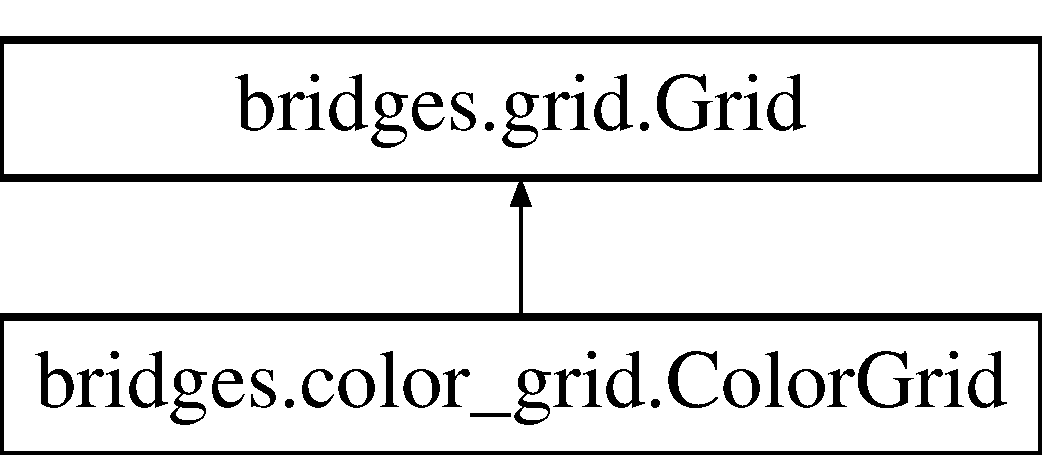
\includegraphics[height=2.000000cm]{classbridges_1_1color__grid_1_1_color_grid}
\end{center}
\end{figure}


\subsection{Detailed Description}
This is a class in B\+R\+I\+D\+G\+ES for representing an (n x n) grid. 

A \hyperlink{classbridges_1_1color__grid_1_1_color_grid}{Color\+Grid} is essentially an image. One can construct an image of a particular size using the Color\+Grid() constructor to be either blank or filled with a particular Color depending on which constructor is called.


\begin{DoxyCode}
grid = new ColorGrid(rows, columns)
grid.set(2, 3, Color(\textcolor{stringliteral}{"lightsalmon"})
\end{DoxyCode}


You can get a \hyperlink{classbridges_1_1color__grid_1_1_color_grid}{Color\+Grid} from an existing Bridges \hyperlink{classbridges_1_1color__grid_1_1_color_grid}{Color\+Grid} assignment using bridges.\+get\+\_\+color\+\_\+grid\+\_\+from\+\_\+assignment(bridges.\+get\+\_\+username(), bridges.\+get\+\_\+assignment\+\_\+id(), 0)

\begin{DoxyAuthor}{Author}
David Burlinson, Matthew Mc\+Quaigue
\end{DoxyAuthor}
\begin{DoxyDate}{Date}
2018, 7/24/19
\end{DoxyDate}
Color grid tutorial at \href{http://bridgesuncc.github.io/tutorials/Grid.html}{\tt http\+://bridgesuncc.\+github.\+io/tutorials/\+Grid.\+html} \subsection*{Public Member Functions}
\begin{DoxyCompactItemize}
\item 
def \hyperlink{classbridges_1_1color__grid_1_1_color_grid_a4dbf23124fdc8edae222c100cf7b9363}{get\+\_\+data\+\_\+structure\+\_\+type} (self)
\begin{DoxyCompactList}\small\item\em Get the data structure type. \end{DoxyCompactList}\item 
def \hyperlink{classbridges_1_1color__grid_1_1_color_grid_aa4b484e518b5fc0c970ea36e8500dbe5}{\+\_\+\+\_\+init\+\_\+\+\_\+}
\begin{DoxyCompactList}\small\item\em Color Grid constructor. \end{DoxyCompactList}\item 
def \hyperlink{classbridges_1_1color__grid_1_1_color_grid_ad2b3ab19751cbf629096a25e31bb7f42}{initialize\+\_\+grid} (self)
\begin{DoxyCompactList}\small\item\em initialize the grid anf populate with base colors \end{DoxyCompactList}\item 
def \hyperlink{classbridges_1_1color__grid_1_1_color_grid_a746dde66b828253bd0dfb32c906729fe}{set}
\begin{DoxyCompactList}\small\item\em Set the (row, col) element in the color grid. \end{DoxyCompactList}\item 
def \hyperlink{classbridges_1_1color__grid_1_1_color_grid_a48ded4391e60e4f42213fb3711730614}{get\+\_\+rle} (self)
\begin{DoxyCompactList}\small\item\em Get the run length encoding of color grid. \end{DoxyCompactList}\item 
def \hyperlink{classbridges_1_1color__grid_1_1_color_grid_ab6685633fe237eb118cf2db2f624cd60}{get\+\_\+raw} (self)
\begin{DoxyCompactList}\small\item\em Get raw encoding of color grid. \end{DoxyCompactList}\item 
def \hyperlink{classbridges_1_1color__grid_1_1_color_grid_afda80f44711e0c32c96161d1e681d788}{get\+\_\+data\+\_\+structure\+\_\+representation} (self)
\begin{DoxyCompactList}\small\item\em Get the J\+S\+ON representation of the color grid. \end{DoxyCompactList}\end{DoxyCompactItemize}
\subsection*{Public Attributes}
\begin{DoxyCompactItemize}
\item 
\hyperlink{classbridges_1_1color__grid_1_1_color_grid_af7c28369f01fb4dfc82a5824583a6dbf}{base\+\_\+color}
\item 
\hyperlink{classbridges_1_1color__grid_1_1_color_grid_af248634de8b3d7b92feef01eed40821b}{grid\+\_\+size}
\end{DoxyCompactItemize}
\subsection*{Static Public Attributes}
\begin{DoxyCompactItemize}
\item 
\hyperlink{classbridges_1_1color__grid_1_1_color_grid_ad2db62703be80114e46b490ff02f8bd9}{base\+Color} = \hyperlink{classbridges_1_1color_1_1_color}{Color}(r=0, g=0, b=0, a=1.\+0)
\end{DoxyCompactItemize}


\subsection{Constructor \& Destructor Documentation}
\mbox{\Hypertarget{classbridges_1_1color__grid_1_1_color_grid_aa4b484e518b5fc0c970ea36e8500dbe5}\label{classbridges_1_1color__grid_1_1_color_grid_aa4b484e518b5fc0c970ea36e8500dbe5}} 
\index{bridges\+::color\+\_\+grid\+::\+Color\+Grid@{bridges\+::color\+\_\+grid\+::\+Color\+Grid}!\+\_\+\+\_\+init\+\_\+\+\_\+@{\+\_\+\+\_\+init\+\_\+\+\_\+}}
\index{\+\_\+\+\_\+init\+\_\+\+\_\+@{\+\_\+\+\_\+init\+\_\+\+\_\+}!bridges\+::color\+\_\+grid\+::\+Color\+Grid@{bridges\+::color\+\_\+grid\+::\+Color\+Grid}}
\subsubsection{\texorpdfstring{\+\_\+\+\_\+init\+\_\+\+\_\+()}{\_\_init\_\_()}}
{\footnotesize\ttfamily def bridges.\+color\+\_\+grid.\+Color\+Grid.\+\_\+\+\_\+init\+\_\+\+\_\+ (\begin{DoxyParamCaption}\item[{}]{self,  }\item[{}]{rows }\end{DoxyParamCaption})}



Color Grid constructor. 


\begin{DoxyParams}{Parameters}
{\em rows} & number of rows in the grid \\
\hline
{\em cols} & number of columns in the grid \\
\hline
{\em color} & base color of the each grid pixel \\
\hline
\end{DoxyParams}
\begin{DoxyReturn}{Returns}


None 
\end{DoxyReturn}


\subsection{Member Function Documentation}
\mbox{\Hypertarget{classbridges_1_1color__grid_1_1_color_grid_afda80f44711e0c32c96161d1e681d788}\label{classbridges_1_1color__grid_1_1_color_grid_afda80f44711e0c32c96161d1e681d788}} 
\index{bridges\+::color\+\_\+grid\+::\+Color\+Grid@{bridges\+::color\+\_\+grid\+::\+Color\+Grid}!get\+\_\+data\+\_\+structure\+\_\+representation@{get\+\_\+data\+\_\+structure\+\_\+representation}}
\index{get\+\_\+data\+\_\+structure\+\_\+representation@{get\+\_\+data\+\_\+structure\+\_\+representation}!bridges\+::color\+\_\+grid\+::\+Color\+Grid@{bridges\+::color\+\_\+grid\+::\+Color\+Grid}}
\subsubsection{\texorpdfstring{get\+\_\+data\+\_\+structure\+\_\+representation()}{get\_data\_structure\_representation()}}
{\footnotesize\ttfamily def bridges.\+color\+\_\+grid.\+Color\+Grid.\+get\+\_\+data\+\_\+structure\+\_\+representation (\begin{DoxyParamCaption}\item[{}]{self,  }\item[{}]{dict }\end{DoxyParamCaption})}



Get the J\+S\+ON representation of the color grid. 

\begin{DoxyReturn}{Returns}


str representing the json of the color grid 
\end{DoxyReturn}
\mbox{\Hypertarget{classbridges_1_1color__grid_1_1_color_grid_a4dbf23124fdc8edae222c100cf7b9363}\label{classbridges_1_1color__grid_1_1_color_grid_a4dbf23124fdc8edae222c100cf7b9363}} 
\index{bridges\+::color\+\_\+grid\+::\+Color\+Grid@{bridges\+::color\+\_\+grid\+::\+Color\+Grid}!get\+\_\+data\+\_\+structure\+\_\+type@{get\+\_\+data\+\_\+structure\+\_\+type}}
\index{get\+\_\+data\+\_\+structure\+\_\+type@{get\+\_\+data\+\_\+structure\+\_\+type}!bridges\+::color\+\_\+grid\+::\+Color\+Grid@{bridges\+::color\+\_\+grid\+::\+Color\+Grid}}
\subsubsection{\texorpdfstring{get\+\_\+data\+\_\+structure\+\_\+type()}{get\_data\_structure\_type()}}
{\footnotesize\ttfamily def bridges.\+color\+\_\+grid.\+Color\+Grid.\+get\+\_\+data\+\_\+structure\+\_\+type (\begin{DoxyParamCaption}\item[{}]{self,  }\item[{}]{str }\end{DoxyParamCaption})}



Get the data structure type. 

\begin{DoxyReturn}{Returns}


str data structure type 
\end{DoxyReturn}
\mbox{\Hypertarget{classbridges_1_1color__grid_1_1_color_grid_ab6685633fe237eb118cf2db2f624cd60}\label{classbridges_1_1color__grid_1_1_color_grid_ab6685633fe237eb118cf2db2f624cd60}} 
\index{bridges\+::color\+\_\+grid\+::\+Color\+Grid@{bridges\+::color\+\_\+grid\+::\+Color\+Grid}!get\+\_\+raw@{get\+\_\+raw}}
\index{get\+\_\+raw@{get\+\_\+raw}!bridges\+::color\+\_\+grid\+::\+Color\+Grid@{bridges\+::color\+\_\+grid\+::\+Color\+Grid}}
\subsubsection{\texorpdfstring{get\+\_\+raw()}{get\_raw()}}
{\footnotesize\ttfamily def bridges.\+color\+\_\+grid.\+Color\+Grid.\+get\+\_\+raw (\begin{DoxyParamCaption}\item[{}]{self,  }\item[{}]{bytearray }\end{DoxyParamCaption})}



Get raw encoding of color grid. 

\begin{DoxyReturn}{Returns}


bytearray representing the colors of grid cells 
\end{DoxyReturn}
\mbox{\Hypertarget{classbridges_1_1color__grid_1_1_color_grid_a48ded4391e60e4f42213fb3711730614}\label{classbridges_1_1color__grid_1_1_color_grid_a48ded4391e60e4f42213fb3711730614}} 
\index{bridges\+::color\+\_\+grid\+::\+Color\+Grid@{bridges\+::color\+\_\+grid\+::\+Color\+Grid}!get\+\_\+rle@{get\+\_\+rle}}
\index{get\+\_\+rle@{get\+\_\+rle}!bridges\+::color\+\_\+grid\+::\+Color\+Grid@{bridges\+::color\+\_\+grid\+::\+Color\+Grid}}
\subsubsection{\texorpdfstring{get\+\_\+rle()}{get\_rle()}}
{\footnotesize\ttfamily def bridges.\+color\+\_\+grid.\+Color\+Grid.\+get\+\_\+rle (\begin{DoxyParamCaption}\item[{}]{self,  }\item[{}]{bytearray }\end{DoxyParamCaption})}



Get the run length encoding of color grid. 

\begin{DoxyReturn}{Returns}


bytearray 
\end{DoxyReturn}
\mbox{\Hypertarget{classbridges_1_1color__grid_1_1_color_grid_ad2b3ab19751cbf629096a25e31bb7f42}\label{classbridges_1_1color__grid_1_1_color_grid_ad2b3ab19751cbf629096a25e31bb7f42}} 
\index{bridges\+::color\+\_\+grid\+::\+Color\+Grid@{bridges\+::color\+\_\+grid\+::\+Color\+Grid}!initialize\+\_\+grid@{initialize\+\_\+grid}}
\index{initialize\+\_\+grid@{initialize\+\_\+grid}!bridges\+::color\+\_\+grid\+::\+Color\+Grid@{bridges\+::color\+\_\+grid\+::\+Color\+Grid}}
\subsubsection{\texorpdfstring{initialize\+\_\+grid()}{initialize\_grid()}}
{\footnotesize\ttfamily def bridges.\+color\+\_\+grid.\+Color\+Grid.\+initialize\+\_\+grid (\begin{DoxyParamCaption}\item[{}]{self,  }\item[{}]{None }\end{DoxyParamCaption})}



initialize the grid anf populate with base colors 

\begin{DoxyReturn}{Returns}


None 
\end{DoxyReturn}
\mbox{\Hypertarget{classbridges_1_1color__grid_1_1_color_grid_a746dde66b828253bd0dfb32c906729fe}\label{classbridges_1_1color__grid_1_1_color_grid_a746dde66b828253bd0dfb32c906729fe}} 
\index{bridges\+::color\+\_\+grid\+::\+Color\+Grid@{bridges\+::color\+\_\+grid\+::\+Color\+Grid}!set@{set}}
\index{set@{set}!bridges\+::color\+\_\+grid\+::\+Color\+Grid@{bridges\+::color\+\_\+grid\+::\+Color\+Grid}}
\subsubsection{\texorpdfstring{set()}{set()}}
{\footnotesize\ttfamily def bridges.\+color\+\_\+grid.\+Color\+Grid.\+set (\begin{DoxyParamCaption}\item[{}]{self,  }\item[{}]{row }\end{DoxyParamCaption})}



Set the (row, col) element in the color grid. 


\begin{DoxyParams}{Parameters}
{\em row} & which row to access \\
\hline
{\em col} & which col to access \\
\hline
{\em color} & background color for the cell at row,col \\
\hline
\end{DoxyParams}
\begin{DoxyReturn}{Returns}


None 
\end{DoxyReturn}


\subsection{Member Data Documentation}
\mbox{\Hypertarget{classbridges_1_1color__grid_1_1_color_grid_af7c28369f01fb4dfc82a5824583a6dbf}\label{classbridges_1_1color__grid_1_1_color_grid_af7c28369f01fb4dfc82a5824583a6dbf}} 
\index{bridges\+::color\+\_\+grid\+::\+Color\+Grid@{bridges\+::color\+\_\+grid\+::\+Color\+Grid}!base\+\_\+color@{base\+\_\+color}}
\index{base\+\_\+color@{base\+\_\+color}!bridges\+::color\+\_\+grid\+::\+Color\+Grid@{bridges\+::color\+\_\+grid\+::\+Color\+Grid}}
\subsubsection{\texorpdfstring{base\+\_\+color}{base\_color}}
{\footnotesize\ttfamily bridges.\+color\+\_\+grid.\+Color\+Grid.\+base\+\_\+color}

\mbox{\Hypertarget{classbridges_1_1color__grid_1_1_color_grid_ad2db62703be80114e46b490ff02f8bd9}\label{classbridges_1_1color__grid_1_1_color_grid_ad2db62703be80114e46b490ff02f8bd9}} 
\index{bridges\+::color\+\_\+grid\+::\+Color\+Grid@{bridges\+::color\+\_\+grid\+::\+Color\+Grid}!base\+Color@{base\+Color}}
\index{base\+Color@{base\+Color}!bridges\+::color\+\_\+grid\+::\+Color\+Grid@{bridges\+::color\+\_\+grid\+::\+Color\+Grid}}
\subsubsection{\texorpdfstring{base\+Color}{baseColor}}
{\footnotesize\ttfamily bridges.\+color\+\_\+grid.\+Color\+Grid.\+base\+Color = \hyperlink{classbridges_1_1color_1_1_color}{Color}(r=0, g=0, b=0, a=1.\+0)\hspace{0.3cm}{\ttfamily [static]}}

\mbox{\Hypertarget{classbridges_1_1color__grid_1_1_color_grid_af248634de8b3d7b92feef01eed40821b}\label{classbridges_1_1color__grid_1_1_color_grid_af248634de8b3d7b92feef01eed40821b}} 
\index{bridges\+::color\+\_\+grid\+::\+Color\+Grid@{bridges\+::color\+\_\+grid\+::\+Color\+Grid}!grid\+\_\+size@{grid\+\_\+size}}
\index{grid\+\_\+size@{grid\+\_\+size}!bridges\+::color\+\_\+grid\+::\+Color\+Grid@{bridges\+::color\+\_\+grid\+::\+Color\+Grid}}
\subsubsection{\texorpdfstring{grid\+\_\+size}{grid\_size}}
{\footnotesize\ttfamily bridges.\+color\+\_\+grid.\+Color\+Grid.\+grid\+\_\+size}



The documentation for this class was generated from the following file\+:\begin{DoxyCompactItemize}
\item 
/home/erik/work/bridges/bridges-\/python/bridges/\hyperlink{color__grid_8py}{color\+\_\+grid.\+py}\end{DoxyCompactItemize}

\hypertarget{classbridges_1_1connector_1_1_connector}{}\section{bridges.\+connector.\+Connector Class Reference}
\label{classbridges_1_1connector_1_1_connector}\index{bridges.\+connector.\+Connector@{bridges.\+connector.\+Connector}}


\subsection{Detailed Description}
This is a class for handling calls to the B\+R\+I\+D\+G\+ES server to transmit J\+S\+ON to the server and subsequent visualization. 

It is not intended for external use \subsection*{Public Member Functions}
\begin{DoxyCompactItemize}
\item 
def \hyperlink{classbridges_1_1connector_1_1_connector_a2d5af7535b60c92433f2333951b7ea69}{\+\_\+\+\_\+init\+\_\+\+\_\+} (self, \hyperlink{classbridges_1_1connector_1_1_connector_a3b577c34402fea1910f56fd9cac51c07}{key}, \hyperlink{classbridges_1_1connector_1_1_connector_af2f4f996092cf63a5e7940ca93a2c6b7}{username}, \hyperlink{classbridges_1_1connector_1_1_connector_a2df020c062b6224d4eeb2c5407c02656}{assignment})
\begin{DoxyCompactList}\small\item\em \hyperlink{classbridges_1_1connector_1_1_connector}{Connector} object constructor. \end{DoxyCompactList}\item 
def \hyperlink{classbridges_1_1connector_1_1_connector_aabe66803d7701015138288c5ceeba81f}{set\+\_\+server} (self, server)
\begin{DoxyCompactList}\small\item\em Set the server based on a keyword for url. \end{DoxyCompactList}\item 
def \hyperlink{classbridges_1_1connector_1_1_connector_a6cfa754618584132754cea9a8bde5282}{set\+\_\+server\+\_\+url} (self, \hyperlink{classbridges_1_1connector_1_1_connector_abcc06e345e43916cf975eb200187d911}{server\+\_\+url})
\item 
def \hyperlink{classbridges_1_1connector_1_1_connector_a1db4c60fd9c2817c2ff237bdfb98e4a9}{get\+\_\+server\+\_\+url} (self)
\item 
def \hyperlink{classbridges_1_1connector_1_1_connector_abfc36138302d5ec49219cb3ccf48439a}{post} (self, url, data)
\item 
def \hyperlink{classbridges_1_1connector_1_1_connector_afcd39dd1f2f37a945e16254e0fed178b}{prepare} (self, url)
\end{DoxyCompactItemize}
\subsection*{Public Attributes}
\begin{DoxyCompactItemize}
\item 
\hyperlink{classbridges_1_1connector_1_1_connector_afeae8bc992dfa4336a6cc766d8414e6f}{key}
\item 
\hyperlink{classbridges_1_1connector_1_1_connector_adeb8d1b493eae70c24127fb175e1bfe7}{username}
\item 
\hyperlink{classbridges_1_1connector_1_1_connector_a2df020c062b6224d4eeb2c5407c02656}{assignment}
\item 
\hyperlink{classbridges_1_1connector_1_1_connector_abcc06e345e43916cf975eb200187d911}{server\+\_\+url}
\end{DoxyCompactItemize}
\subsection*{Static Public Attributes}
\begin{DoxyCompactItemize}
\item 
string \hyperlink{classbridges_1_1connector_1_1_connector_a10c26bfaf2718f837e7bddfd7715b729}{server\+\_\+url\+\_\+live} = \char`\"{}http\+://bridges-\/cs.\+herokuapp.\+com\char`\"{}
\item 
string \hyperlink{classbridges_1_1connector_1_1_connector_ab5146d539819322f0b0e121a56356ba2}{server\+\_\+type} = \char`\"{}application\char`\"{}
\item 
string \hyperlink{classbridges_1_1connector_1_1_connector_a9048518314ac4902eda88f8457154b63}{server\+\_\+url\+\_\+clone} = \char`\"{}http\+://bridges-\/clone.\+herokuapp.\+com\char`\"{}
\item 
string \hyperlink{classbridges_1_1connector_1_1_connector_a7d58b50fbd7d10f805957ec620135ef7}{server\+\_\+url\+\_\+local} = \char`\"{}http\+://127.\+0.\+0.\+1\+:3000\char`\"{}
\item 
string \hyperlink{classbridges_1_1connector_1_1_connector_ad2c0c9e4bff85bbfb05816fc9a3515fc}{server\+\_\+url\+\_\+game} = \char`\"{}http\+://bridges-\/games.\+herokuapp.\+com\char`\"{}
\item 
string \hyperlink{classbridges_1_1connector_1_1_connector_a3b577c34402fea1910f56fd9cac51c07}{key} = \char`\"{}\char`\"{}
\item 
string \hyperlink{classbridges_1_1connector_1_1_connector_af2f4f996092cf63a5e7940ca93a2c6b7}{username} = \char`\"{}\char`\"{}
\item 
int \hyperlink{classbridges_1_1connector_1_1_connector_ad137981eae887e1f050216edb7670d35}{pattern\+\_\+found} = 0
\item 
bool \hyperlink{classbridges_1_1connector_1_1_connector_a05ea0150f79561e26b725654fe8ff7dc}{debug} = False
\end{DoxyCompactItemize}


\subsection{Constructor \& Destructor Documentation}
\mbox{\Hypertarget{classbridges_1_1connector_1_1_connector_a2d5af7535b60c92433f2333951b7ea69}\label{classbridges_1_1connector_1_1_connector_a2d5af7535b60c92433f2333951b7ea69}} 
\index{bridges\+::connector\+::\+Connector@{bridges\+::connector\+::\+Connector}!\+\_\+\+\_\+init\+\_\+\+\_\+@{\+\_\+\+\_\+init\+\_\+\+\_\+}}
\index{\+\_\+\+\_\+init\+\_\+\+\_\+@{\+\_\+\+\_\+init\+\_\+\+\_\+}!bridges\+::connector\+::\+Connector@{bridges\+::connector\+::\+Connector}}
\subsubsection{\texorpdfstring{\+\_\+\+\_\+init\+\_\+\+\_\+()}{\_\_init\_\_()}}
{\footnotesize\ttfamily def bridges.\+connector.\+Connector.\+\_\+\+\_\+init\+\_\+\+\_\+ (\begin{DoxyParamCaption}\item[{}]{self,  }\item[{}]{key,  }\item[{}]{username,  }\item[{}]{assignment }\end{DoxyParamCaption})}



\hyperlink{classbridges_1_1connector_1_1_connector}{Connector} object constructor. 


\begin{DoxyParams}{Parameters}
{\em key} & is the user\+\_\+key \\
\hline
{\em username} & is students username \\
\hline
{\em assignment} & is the assignment number for the assignment \\
\hline
\end{DoxyParams}


\subsection{Member Function Documentation}
\mbox{\Hypertarget{classbridges_1_1connector_1_1_connector_a1db4c60fd9c2817c2ff237bdfb98e4a9}\label{classbridges_1_1connector_1_1_connector_a1db4c60fd9c2817c2ff237bdfb98e4a9}} 
\index{bridges\+::connector\+::\+Connector@{bridges\+::connector\+::\+Connector}!get\+\_\+server\+\_\+url@{get\+\_\+server\+\_\+url}}
\index{get\+\_\+server\+\_\+url@{get\+\_\+server\+\_\+url}!bridges\+::connector\+::\+Connector@{bridges\+::connector\+::\+Connector}}
\subsubsection{\texorpdfstring{get\+\_\+server\+\_\+url()}{get\_server\_url()}}
{\footnotesize\ttfamily def bridges.\+connector.\+Connector.\+get\+\_\+server\+\_\+url (\begin{DoxyParamCaption}\item[{}]{self }\end{DoxyParamCaption})}

\mbox{\Hypertarget{classbridges_1_1connector_1_1_connector_abfc36138302d5ec49219cb3ccf48439a}\label{classbridges_1_1connector_1_1_connector_abfc36138302d5ec49219cb3ccf48439a}} 
\index{bridges\+::connector\+::\+Connector@{bridges\+::connector\+::\+Connector}!post@{post}}
\index{post@{post}!bridges\+::connector\+::\+Connector@{bridges\+::connector\+::\+Connector}}
\subsubsection{\texorpdfstring{post()}{post()}}
{\footnotesize\ttfamily def bridges.\+connector.\+Connector.\+post (\begin{DoxyParamCaption}\item[{}]{self,  }\item[{}]{url,  }\item[{}]{data }\end{DoxyParamCaption})}

\mbox{\Hypertarget{classbridges_1_1connector_1_1_connector_afcd39dd1f2f37a945e16254e0fed178b}\label{classbridges_1_1connector_1_1_connector_afcd39dd1f2f37a945e16254e0fed178b}} 
\index{bridges\+::connector\+::\+Connector@{bridges\+::connector\+::\+Connector}!prepare@{prepare}}
\index{prepare@{prepare}!bridges\+::connector\+::\+Connector@{bridges\+::connector\+::\+Connector}}
\subsubsection{\texorpdfstring{prepare()}{prepare()}}
{\footnotesize\ttfamily def bridges.\+connector.\+Connector.\+prepare (\begin{DoxyParamCaption}\item[{}]{self,  }\item[{}]{url }\end{DoxyParamCaption})}

\mbox{\Hypertarget{classbridges_1_1connector_1_1_connector_aabe66803d7701015138288c5ceeba81f}\label{classbridges_1_1connector_1_1_connector_aabe66803d7701015138288c5ceeba81f}} 
\index{bridges\+::connector\+::\+Connector@{bridges\+::connector\+::\+Connector}!set\+\_\+server@{set\+\_\+server}}
\index{set\+\_\+server@{set\+\_\+server}!bridges\+::connector\+::\+Connector@{bridges\+::connector\+::\+Connector}}
\subsubsection{\texorpdfstring{set\+\_\+server()}{set\_server()}}
{\footnotesize\ttfamily def bridges.\+connector.\+Connector.\+set\+\_\+server (\begin{DoxyParamCaption}\item[{}]{self,  }\item[{}]{server }\end{DoxyParamCaption})}



Set the server based on a keyword for url. 


\begin{DoxyParams}{Parameters}
{\em server} & is one of the three string keywords(\textquotesingle{}live\textquotesingle{}, \textquotesingle{}clone\textquotesingle{}, \textquotesingle{}local\textquotesingle{}) that is passed to change the server that the bridges visualization will be sent to \\
\hline
\end{DoxyParams}
\mbox{\Hypertarget{classbridges_1_1connector_1_1_connector_a6cfa754618584132754cea9a8bde5282}\label{classbridges_1_1connector_1_1_connector_a6cfa754618584132754cea9a8bde5282}} 
\index{bridges\+::connector\+::\+Connector@{bridges\+::connector\+::\+Connector}!set\+\_\+server\+\_\+url@{set\+\_\+server\+\_\+url}}
\index{set\+\_\+server\+\_\+url@{set\+\_\+server\+\_\+url}!bridges\+::connector\+::\+Connector@{bridges\+::connector\+::\+Connector}}
\subsubsection{\texorpdfstring{set\+\_\+server\+\_\+url()}{set\_server\_url()}}
{\footnotesize\ttfamily def bridges.\+connector.\+Connector.\+set\+\_\+server\+\_\+url (\begin{DoxyParamCaption}\item[{}]{self,  }\item[{}]{server\+\_\+url }\end{DoxyParamCaption})}



\subsection{Member Data Documentation}
\mbox{\Hypertarget{classbridges_1_1connector_1_1_connector_a2df020c062b6224d4eeb2c5407c02656}\label{classbridges_1_1connector_1_1_connector_a2df020c062b6224d4eeb2c5407c02656}} 
\index{bridges\+::connector\+::\+Connector@{bridges\+::connector\+::\+Connector}!assignment@{assignment}}
\index{assignment@{assignment}!bridges\+::connector\+::\+Connector@{bridges\+::connector\+::\+Connector}}
\subsubsection{\texorpdfstring{assignment}{assignment}}
{\footnotesize\ttfamily bridges.\+connector.\+Connector.\+assignment}

\mbox{\Hypertarget{classbridges_1_1connector_1_1_connector_a05ea0150f79561e26b725654fe8ff7dc}\label{classbridges_1_1connector_1_1_connector_a05ea0150f79561e26b725654fe8ff7dc}} 
\index{bridges\+::connector\+::\+Connector@{bridges\+::connector\+::\+Connector}!debug@{debug}}
\index{debug@{debug}!bridges\+::connector\+::\+Connector@{bridges\+::connector\+::\+Connector}}
\subsubsection{\texorpdfstring{debug}{debug}}
{\footnotesize\ttfamily bool bridges.\+connector.\+Connector.\+debug = False\hspace{0.3cm}{\ttfamily [static]}}

\mbox{\Hypertarget{classbridges_1_1connector_1_1_connector_a3b577c34402fea1910f56fd9cac51c07}\label{classbridges_1_1connector_1_1_connector_a3b577c34402fea1910f56fd9cac51c07}} 
\index{bridges\+::connector\+::\+Connector@{bridges\+::connector\+::\+Connector}!key@{key}}
\index{key@{key}!bridges\+::connector\+::\+Connector@{bridges\+::connector\+::\+Connector}}
\subsubsection{\texorpdfstring{key}{key}\hspace{0.1cm}{\footnotesize\ttfamily [1/2]}}
{\footnotesize\ttfamily string bridges.\+connector.\+Connector.\+key = \char`\"{}\char`\"{}\hspace{0.3cm}{\ttfamily [static]}}

\mbox{\Hypertarget{classbridges_1_1connector_1_1_connector_afeae8bc992dfa4336a6cc766d8414e6f}\label{classbridges_1_1connector_1_1_connector_afeae8bc992dfa4336a6cc766d8414e6f}} 
\index{bridges\+::connector\+::\+Connector@{bridges\+::connector\+::\+Connector}!key@{key}}
\index{key@{key}!bridges\+::connector\+::\+Connector@{bridges\+::connector\+::\+Connector}}
\subsubsection{\texorpdfstring{key}{key}\hspace{0.1cm}{\footnotesize\ttfamily [2/2]}}
{\footnotesize\ttfamily bridges.\+connector.\+Connector.\+key}

\mbox{\Hypertarget{classbridges_1_1connector_1_1_connector_ad137981eae887e1f050216edb7670d35}\label{classbridges_1_1connector_1_1_connector_ad137981eae887e1f050216edb7670d35}} 
\index{bridges\+::connector\+::\+Connector@{bridges\+::connector\+::\+Connector}!pattern\+\_\+found@{pattern\+\_\+found}}
\index{pattern\+\_\+found@{pattern\+\_\+found}!bridges\+::connector\+::\+Connector@{bridges\+::connector\+::\+Connector}}
\subsubsection{\texorpdfstring{pattern\+\_\+found}{pattern\_found}}
{\footnotesize\ttfamily int bridges.\+connector.\+Connector.\+pattern\+\_\+found = 0\hspace{0.3cm}{\ttfamily [static]}}

\mbox{\Hypertarget{classbridges_1_1connector_1_1_connector_ab5146d539819322f0b0e121a56356ba2}\label{classbridges_1_1connector_1_1_connector_ab5146d539819322f0b0e121a56356ba2}} 
\index{bridges\+::connector\+::\+Connector@{bridges\+::connector\+::\+Connector}!server\+\_\+type@{server\+\_\+type}}
\index{server\+\_\+type@{server\+\_\+type}!bridges\+::connector\+::\+Connector@{bridges\+::connector\+::\+Connector}}
\subsubsection{\texorpdfstring{server\+\_\+type}{server\_type}}
{\footnotesize\ttfamily string bridges.\+connector.\+Connector.\+server\+\_\+type = \char`\"{}application\char`\"{}\hspace{0.3cm}{\ttfamily [static]}}

\mbox{\Hypertarget{classbridges_1_1connector_1_1_connector_abcc06e345e43916cf975eb200187d911}\label{classbridges_1_1connector_1_1_connector_abcc06e345e43916cf975eb200187d911}} 
\index{bridges\+::connector\+::\+Connector@{bridges\+::connector\+::\+Connector}!server\+\_\+url@{server\+\_\+url}}
\index{server\+\_\+url@{server\+\_\+url}!bridges\+::connector\+::\+Connector@{bridges\+::connector\+::\+Connector}}
\subsubsection{\texorpdfstring{server\+\_\+url}{server\_url}}
{\footnotesize\ttfamily bridges.\+connector.\+Connector.\+server\+\_\+url}

\mbox{\Hypertarget{classbridges_1_1connector_1_1_connector_a9048518314ac4902eda88f8457154b63}\label{classbridges_1_1connector_1_1_connector_a9048518314ac4902eda88f8457154b63}} 
\index{bridges\+::connector\+::\+Connector@{bridges\+::connector\+::\+Connector}!server\+\_\+url\+\_\+clone@{server\+\_\+url\+\_\+clone}}
\index{server\+\_\+url\+\_\+clone@{server\+\_\+url\+\_\+clone}!bridges\+::connector\+::\+Connector@{bridges\+::connector\+::\+Connector}}
\subsubsection{\texorpdfstring{server\+\_\+url\+\_\+clone}{server\_url\_clone}}
{\footnotesize\ttfamily string bridges.\+connector.\+Connector.\+server\+\_\+url\+\_\+clone = \char`\"{}http\+://bridges-\/clone.\+herokuapp.\+com\char`\"{}\hspace{0.3cm}{\ttfamily [static]}}

\mbox{\Hypertarget{classbridges_1_1connector_1_1_connector_ad2c0c9e4bff85bbfb05816fc9a3515fc}\label{classbridges_1_1connector_1_1_connector_ad2c0c9e4bff85bbfb05816fc9a3515fc}} 
\index{bridges\+::connector\+::\+Connector@{bridges\+::connector\+::\+Connector}!server\+\_\+url\+\_\+game@{server\+\_\+url\+\_\+game}}
\index{server\+\_\+url\+\_\+game@{server\+\_\+url\+\_\+game}!bridges\+::connector\+::\+Connector@{bridges\+::connector\+::\+Connector}}
\subsubsection{\texorpdfstring{server\+\_\+url\+\_\+game}{server\_url\_game}}
{\footnotesize\ttfamily string bridges.\+connector.\+Connector.\+server\+\_\+url\+\_\+game = \char`\"{}http\+://bridges-\/games.\+herokuapp.\+com\char`\"{}\hspace{0.3cm}{\ttfamily [static]}}

\mbox{\Hypertarget{classbridges_1_1connector_1_1_connector_a10c26bfaf2718f837e7bddfd7715b729}\label{classbridges_1_1connector_1_1_connector_a10c26bfaf2718f837e7bddfd7715b729}} 
\index{bridges\+::connector\+::\+Connector@{bridges\+::connector\+::\+Connector}!server\+\_\+url\+\_\+live@{server\+\_\+url\+\_\+live}}
\index{server\+\_\+url\+\_\+live@{server\+\_\+url\+\_\+live}!bridges\+::connector\+::\+Connector@{bridges\+::connector\+::\+Connector}}
\subsubsection{\texorpdfstring{server\+\_\+url\+\_\+live}{server\_url\_live}}
{\footnotesize\ttfamily string bridges.\+connector.\+Connector.\+server\+\_\+url\+\_\+live = \char`\"{}http\+://bridges-\/cs.\+herokuapp.\+com\char`\"{}\hspace{0.3cm}{\ttfamily [static]}}

\mbox{\Hypertarget{classbridges_1_1connector_1_1_connector_a7d58b50fbd7d10f805957ec620135ef7}\label{classbridges_1_1connector_1_1_connector_a7d58b50fbd7d10f805957ec620135ef7}} 
\index{bridges\+::connector\+::\+Connector@{bridges\+::connector\+::\+Connector}!server\+\_\+url\+\_\+local@{server\+\_\+url\+\_\+local}}
\index{server\+\_\+url\+\_\+local@{server\+\_\+url\+\_\+local}!bridges\+::connector\+::\+Connector@{bridges\+::connector\+::\+Connector}}
\subsubsection{\texorpdfstring{server\+\_\+url\+\_\+local}{server\_url\_local}}
{\footnotesize\ttfamily string bridges.\+connector.\+Connector.\+server\+\_\+url\+\_\+local = \char`\"{}http\+://127.\+0.\+0.\+1\+:3000\char`\"{}\hspace{0.3cm}{\ttfamily [static]}}

\mbox{\Hypertarget{classbridges_1_1connector_1_1_connector_af2f4f996092cf63a5e7940ca93a2c6b7}\label{classbridges_1_1connector_1_1_connector_af2f4f996092cf63a5e7940ca93a2c6b7}} 
\index{bridges\+::connector\+::\+Connector@{bridges\+::connector\+::\+Connector}!username@{username}}
\index{username@{username}!bridges\+::connector\+::\+Connector@{bridges\+::connector\+::\+Connector}}
\subsubsection{\texorpdfstring{username}{username}\hspace{0.1cm}{\footnotesize\ttfamily [1/2]}}
{\footnotesize\ttfamily string bridges.\+connector.\+Connector.\+username = \char`\"{}\char`\"{}\hspace{0.3cm}{\ttfamily [static]}}

\mbox{\Hypertarget{classbridges_1_1connector_1_1_connector_adeb8d1b493eae70c24127fb175e1bfe7}\label{classbridges_1_1connector_1_1_connector_adeb8d1b493eae70c24127fb175e1bfe7}} 
\index{bridges\+::connector\+::\+Connector@{bridges\+::connector\+::\+Connector}!username@{username}}
\index{username@{username}!bridges\+::connector\+::\+Connector@{bridges\+::connector\+::\+Connector}}
\subsubsection{\texorpdfstring{username}{username}\hspace{0.1cm}{\footnotesize\ttfamily [2/2]}}
{\footnotesize\ttfamily bridges.\+connector.\+Connector.\+username}



The documentation for this class was generated from the following file\+:\begin{DoxyCompactItemize}
\item 
/home/erik/work/bridges/bridges-\/python/bridges/\hyperlink{connector_8py}{connector.\+py}\end{DoxyCompactItemize}

\hypertarget{classbridges_1_1dl__element_1_1_d_lelement}{}\section{bridges.\+dl\+\_\+element.\+D\+Lelement Class Reference}
\label{classbridges_1_1dl__element_1_1_d_lelement}\index{bridges.\+dl\+\_\+element.\+D\+Lelement@{bridges.\+dl\+\_\+element.\+D\+Lelement}}
Inheritance diagram for bridges.\+dl\+\_\+element.\+D\+Lelement\+:\begin{figure}[H]
\begin{center}
\leavevmode
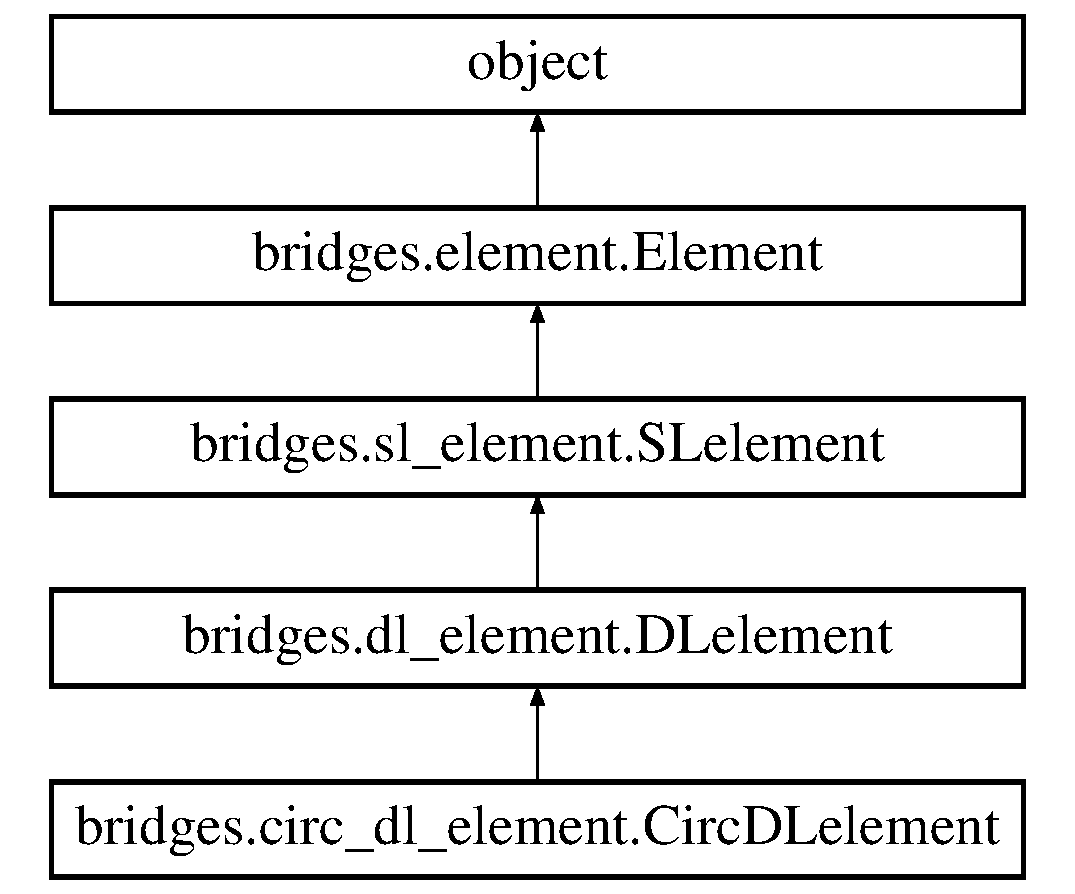
\includegraphics[height=4.000000cm]{classbridges_1_1dl__element_1_1_d_lelement}
\end{center}
\end{figure}


\subsection{Detailed Description}
This class is used to create doubly linked element objects. 

This class extends Element and takes a generic parameter $<$\+E$>$ representing application specific data. This element forms the basic building block for doubly linked lists. Doubly linked elements have two links, \char`\"{}next\char`\"{} and \char`\"{}previous\char`\"{}, that point to the previous and succeeding nodes along the list.

Elements contain a visualizer (Element\+Visualizer) object for setting visual attributes (color, shape, opacity, size), necessary for displaying them in a web browser.

Elements also have a Link\+Visualizer object that is used when they are linked to another element, appropriate for setting link attributes, such as in linked lists, between the current element and its next or previous nodes.

\begin{DoxyAuthor}{Author}
Mihai Mehedint, Kalpathi Subramanian 
\end{DoxyAuthor}
\begin{DoxyDate}{Date}
2018, 6/24/19
\end{DoxyDate}
\begin{DoxySeeAlso}{See also}
Doubly Linked List tutorial \+: \href{http://bridgesuncc.github.io/tutorials/DoublyLinkedList.html}{\tt http\+://bridgesuncc.\+github.\+io/tutorials/\+Doubly\+Linked\+List.\+html} 
\end{DoxySeeAlso}
\subsection*{Public Member Functions}
\begin{DoxyCompactItemize}
\item 
def \hyperlink{classbridges_1_1dl__element_1_1_d_lelement_a54256a7be5796b0471cb2655dd971bd5}{\+\_\+\+\_\+init\+\_\+\+\_\+} (self, args, kwargs)
\begin{DoxyCompactList}\small\item\em Constructor for \hyperlink{classbridges_1_1dl__element_1_1_d_lelement}{D\+Lelement}. \end{DoxyCompactList}\item 
def \hyperlink{classbridges_1_1dl__element_1_1_d_lelement_a5fb177ed67b75e606ac303f7a972d301}{get\+\_\+data\+\_\+structure\+\_\+type} (self)
\begin{DoxyCompactList}\small\item\em This method gets the data structure type. \end{DoxyCompactList}\item 
def \hyperlink{classbridges_1_1dl__element_1_1_d_lelement_a43077e810ec453c9cd512ba75819e28a}{next} (self)
\begin{DoxyCompactList}\small\item\em Getter for the next element in Dlelement. \end{DoxyCompactList}\item 
def \hyperlink{classbridges_1_1dl__element_1_1_d_lelement_ae46f630cd7384689d4305770e6b2c7c1}{next} (self, el)
\begin{DoxyCompactList}\small\item\em Setter for the next element. \end{DoxyCompactList}\item 
def \hyperlink{classbridges_1_1dl__element_1_1_d_lelement_a66e7c4bfb2216a68744fe58c24e9917f}{prev} (self)
\begin{DoxyCompactList}\small\item\em Getter for the prev element in Dlelement. \end{DoxyCompactList}\item 
def \hyperlink{classbridges_1_1dl__element_1_1_d_lelement_a17c371ec0c38e9555e55551d9be4d185}{prev} (self, el)
\begin{DoxyCompactList}\small\item\em Setter for the prev element. \end{DoxyCompactList}\item 
def \hyperlink{classbridges_1_1dl__element_1_1_d_lelement_abcae653ca8e9590c594910bad148ddf2}{get\+\_\+data\+\_\+structure\+\_\+representation} (self)
\begin{DoxyCompactList}\small\item\em Getter for the json representation of this list. \end{DoxyCompactList}\item 
def \hyperlink{classbridges_1_1dl__element_1_1_d_lelement_a2baa040819283ef3adcda70b630de421}{reverse\+\_\+iterator} (self)
\begin{DoxyCompactList}\small\item\em This iterator is used with range loops. \end{DoxyCompactList}\end{DoxyCompactItemize}
\subsection*{Additional Inherited Members}


\subsection{Constructor \& Destructor Documentation}
\mbox{\Hypertarget{classbridges_1_1dl__element_1_1_d_lelement_a54256a7be5796b0471cb2655dd971bd5}\label{classbridges_1_1dl__element_1_1_d_lelement_a54256a7be5796b0471cb2655dd971bd5}} 
\index{bridges\+::dl\+\_\+element\+::\+D\+Lelement@{bridges\+::dl\+\_\+element\+::\+D\+Lelement}!\+\_\+\+\_\+init\+\_\+\+\_\+@{\+\_\+\+\_\+init\+\_\+\+\_\+}}
\index{\+\_\+\+\_\+init\+\_\+\+\_\+@{\+\_\+\+\_\+init\+\_\+\+\_\+}!bridges\+::dl\+\_\+element\+::\+D\+Lelement@{bridges\+::dl\+\_\+element\+::\+D\+Lelement}}
\subsubsection{\texorpdfstring{\+\_\+\+\_\+init\+\_\+\+\_\+()}{\_\_init\_\_()}}
{\footnotesize\ttfamily def bridges.\+dl\+\_\+element.\+D\+Lelement.\+\_\+\+\_\+init\+\_\+\+\_\+ (\begin{DoxyParamCaption}\item[{}]{self,  }\item[{}]{args,  }\item[{}]{kwargs,  }\item[{}]{None }\end{DoxyParamCaption})}



Constructor for \hyperlink{classbridges_1_1dl__element_1_1_d_lelement}{D\+Lelement}. 

(object) e\+: the genereic application specific object that \hyperlink{classbridges_1_1dl__element_1_1_d_lelement}{D\+Lelement} is holding 
\begin{DoxyParams}{Parameters}
{\em next} & the \hyperlink{classbridges_1_1dl__element_1_1_d_lelement}{D\+Lelement} that should be assigned to the next pointer \\
\hline
{\em prev} & the \hyperlink{classbridges_1_1dl__element_1_1_d_lelement}{D\+Lelement} that should be assigned to the prev pointer (str) label\+: the label for this \hyperlink{classbridges_1_1dl__element_1_1_d_lelement}{D\+Lelement} \\
\hline
\end{DoxyParams}
\begin{DoxyParagraph}{Return}
None 
\end{DoxyParagraph}


\subsection{Member Function Documentation}
\mbox{\Hypertarget{classbridges_1_1dl__element_1_1_d_lelement_abcae653ca8e9590c594910bad148ddf2}\label{classbridges_1_1dl__element_1_1_d_lelement_abcae653ca8e9590c594910bad148ddf2}} 
\index{bridges\+::dl\+\_\+element\+::\+D\+Lelement@{bridges\+::dl\+\_\+element\+::\+D\+Lelement}!get\+\_\+data\+\_\+structure\+\_\+representation@{get\+\_\+data\+\_\+structure\+\_\+representation}}
\index{get\+\_\+data\+\_\+structure\+\_\+representation@{get\+\_\+data\+\_\+structure\+\_\+representation}!bridges\+::dl\+\_\+element\+::\+D\+Lelement@{bridges\+::dl\+\_\+element\+::\+D\+Lelement}}
\subsubsection{\texorpdfstring{get\+\_\+data\+\_\+structure\+\_\+representation()}{get\_data\_structure\_representation()}}
{\footnotesize\ttfamily def bridges.\+dl\+\_\+element.\+D\+Lelement.\+get\+\_\+data\+\_\+structure\+\_\+representation (\begin{DoxyParamCaption}\item[{}]{self,  }\item[{}]{dict }\end{DoxyParamCaption})}



Getter for the json representation of this list. 

\begin{DoxyReturn}{Returns}


dict representing the J\+S\+ON format 
\end{DoxyReturn}
\mbox{\Hypertarget{classbridges_1_1dl__element_1_1_d_lelement_a5fb177ed67b75e606ac303f7a972d301}\label{classbridges_1_1dl__element_1_1_d_lelement_a5fb177ed67b75e606ac303f7a972d301}} 
\index{bridges\+::dl\+\_\+element\+::\+D\+Lelement@{bridges\+::dl\+\_\+element\+::\+D\+Lelement}!get\+\_\+data\+\_\+structure\+\_\+type@{get\+\_\+data\+\_\+structure\+\_\+type}}
\index{get\+\_\+data\+\_\+structure\+\_\+type@{get\+\_\+data\+\_\+structure\+\_\+type}!bridges\+::dl\+\_\+element\+::\+D\+Lelement@{bridges\+::dl\+\_\+element\+::\+D\+Lelement}}
\subsubsection{\texorpdfstring{get\+\_\+data\+\_\+structure\+\_\+type()}{get\_data\_structure\_type()}}
{\footnotesize\ttfamily def bridges.\+dl\+\_\+element.\+D\+Lelement.\+get\+\_\+data\+\_\+structure\+\_\+type (\begin{DoxyParamCaption}\item[{}]{self,  }\item[{}]{str }\end{DoxyParamCaption})}



This method gets the data structure type. 

\begin{DoxyReturn}{Returns}


str representing the data structure type 
\end{DoxyReturn}
\mbox{\Hypertarget{classbridges_1_1dl__element_1_1_d_lelement_a43077e810ec453c9cd512ba75819e28a}\label{classbridges_1_1dl__element_1_1_d_lelement_a43077e810ec453c9cd512ba75819e28a}} 
\index{bridges\+::dl\+\_\+element\+::\+D\+Lelement@{bridges\+::dl\+\_\+element\+::\+D\+Lelement}!next@{next}}
\index{next@{next}!bridges\+::dl\+\_\+element\+::\+D\+Lelement@{bridges\+::dl\+\_\+element\+::\+D\+Lelement}}
\subsubsection{\texorpdfstring{next()}{next()}\hspace{0.1cm}{\footnotesize\ttfamily [1/2]}}
{\footnotesize\ttfamily def bridges.\+dl\+\_\+element.\+D\+Lelement.\+next (\begin{DoxyParamCaption}\item[{}]{self }\end{DoxyParamCaption})}



Getter for the next element in Dlelement. 

\begin{DoxyReturn}{Returns}
element pointed to by this element 
\end{DoxyReturn}
\mbox{\Hypertarget{classbridges_1_1dl__element_1_1_d_lelement_ae46f630cd7384689d4305770e6b2c7c1}\label{classbridges_1_1dl__element_1_1_d_lelement_ae46f630cd7384689d4305770e6b2c7c1}} 
\index{bridges\+::dl\+\_\+element\+::\+D\+Lelement@{bridges\+::dl\+\_\+element\+::\+D\+Lelement}!next@{next}}
\index{next@{next}!bridges\+::dl\+\_\+element\+::\+D\+Lelement@{bridges\+::dl\+\_\+element\+::\+D\+Lelement}}
\subsubsection{\texorpdfstring{next()}{next()}\hspace{0.1cm}{\footnotesize\ttfamily [2/2]}}
{\footnotesize\ttfamily def bridges.\+dl\+\_\+element.\+D\+Lelement.\+next (\begin{DoxyParamCaption}\item[{}]{self,  }\item[{}]{el }\end{DoxyParamCaption})}



Setter for the next element. 


\begin{DoxyParams}{Parameters}
{\em el} & element to be set \\
\hline
\end{DoxyParams}
\begin{DoxyReturn}{Returns}


None 
\end{DoxyReturn}
\mbox{\Hypertarget{classbridges_1_1dl__element_1_1_d_lelement_a66e7c4bfb2216a68744fe58c24e9917f}\label{classbridges_1_1dl__element_1_1_d_lelement_a66e7c4bfb2216a68744fe58c24e9917f}} 
\index{bridges\+::dl\+\_\+element\+::\+D\+Lelement@{bridges\+::dl\+\_\+element\+::\+D\+Lelement}!prev@{prev}}
\index{prev@{prev}!bridges\+::dl\+\_\+element\+::\+D\+Lelement@{bridges\+::dl\+\_\+element\+::\+D\+Lelement}}
\subsubsection{\texorpdfstring{prev()}{prev()}\hspace{0.1cm}{\footnotesize\ttfamily [1/2]}}
{\footnotesize\ttfamily def bridges.\+dl\+\_\+element.\+D\+Lelement.\+prev (\begin{DoxyParamCaption}\item[{}]{self }\end{DoxyParamCaption})}



Getter for the prev element in Dlelement. 

\begin{DoxyReturn}{Returns}
element that is prior to this element 
\end{DoxyReturn}
\mbox{\Hypertarget{classbridges_1_1dl__element_1_1_d_lelement_a17c371ec0c38e9555e55551d9be4d185}\label{classbridges_1_1dl__element_1_1_d_lelement_a17c371ec0c38e9555e55551d9be4d185}} 
\index{bridges\+::dl\+\_\+element\+::\+D\+Lelement@{bridges\+::dl\+\_\+element\+::\+D\+Lelement}!prev@{prev}}
\index{prev@{prev}!bridges\+::dl\+\_\+element\+::\+D\+Lelement@{bridges\+::dl\+\_\+element\+::\+D\+Lelement}}
\subsubsection{\texorpdfstring{prev()}{prev()}\hspace{0.1cm}{\footnotesize\ttfamily [2/2]}}
{\footnotesize\ttfamily def bridges.\+dl\+\_\+element.\+D\+Lelement.\+prev (\begin{DoxyParamCaption}\item[{}]{self,  }\item[{}]{el }\end{DoxyParamCaption})}



Setter for the prev element. 


\begin{DoxyParams}{Parameters}
{\em el} & element to be set\\
\hline
\end{DoxyParams}
\begin{DoxyReturn}{Returns}


None 
\end{DoxyReturn}
\mbox{\Hypertarget{classbridges_1_1dl__element_1_1_d_lelement_a2baa040819283ef3adcda70b630de421}\label{classbridges_1_1dl__element_1_1_d_lelement_a2baa040819283ef3adcda70b630de421}} 
\index{bridges\+::dl\+\_\+element\+::\+D\+Lelement@{bridges\+::dl\+\_\+element\+::\+D\+Lelement}!reverse\+\_\+iterator@{reverse\+\_\+iterator}}
\index{reverse\+\_\+iterator@{reverse\+\_\+iterator}!bridges\+::dl\+\_\+element\+::\+D\+Lelement@{bridges\+::dl\+\_\+element\+::\+D\+Lelement}}
\subsubsection{\texorpdfstring{reverse\+\_\+iterator()}{reverse\_iterator()}}
{\footnotesize\ttfamily def bridges.\+dl\+\_\+element.\+D\+Lelement.\+reverse\+\_\+iterator (\begin{DoxyParamCaption}\item[{}]{self }\end{DoxyParamCaption})}



This iterator is used with range loops. 



The documentation for this class was generated from the following file\+:\begin{DoxyCompactItemize}
\item 
/home/erik/work/bridges/bridges-\/python/bridges/\hyperlink{dl__element_8py}{dl\+\_\+element.\+py}\end{DoxyCompactItemize}

\hypertarget{classbridges_1_1edge_1_1_edge}{}\section{bridges.\+edge.\+Edge Class Reference}
\label{classbridges_1_1edge_1_1_edge}\index{bridges.\+edge.\+Edge@{bridges.\+edge.\+Edge}}


This class is used to represent the edges in a graph and will appear as links in the B\+R\+I\+D\+G\+E\+S graph visualization.  


Inheritance diagram for bridges.\+edge.\+Edge\+:\begin{figure}[H]
\begin{center}
\leavevmode
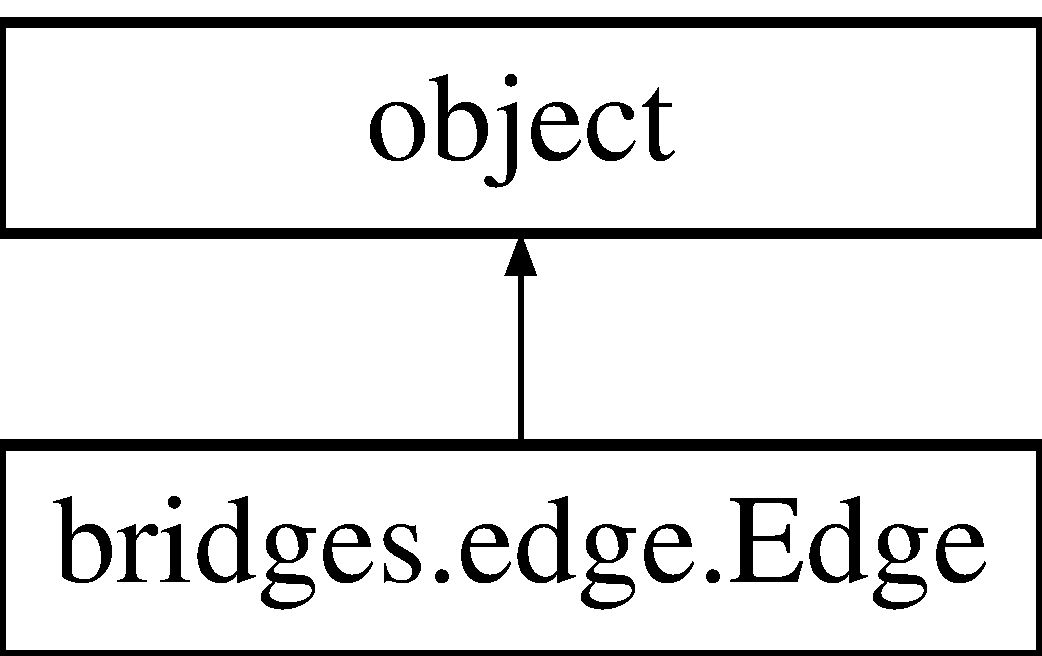
\includegraphics[height=2.000000cm]{classbridges_1_1edge_1_1_edge}
\end{center}
\end{figure}
\subsection*{Public Member Functions}
\begin{DoxyCompactItemize}
\item 
def \hyperlink{classbridges_1_1edge_1_1_edge_aafbac2adad409525c0fc55191fb7cfa8}{\+\_\+\+\_\+init\+\_\+\+\_\+}
\begin{DoxyCompactList}\small\item\em Constructors. \end{DoxyCompactList}\item 
def \hyperlink{classbridges_1_1edge_1_1_edge_ac8dfd60ebfa380ac02b6e9fd8bcb13a1}{set\+\_\+weight} (self, wt)
\begin{DoxyCompactList}\small\item\em Set edge weight to \char`\"{}wt\char`\"{}. \end{DoxyCompactList}\item 
def \hyperlink{classbridges_1_1edge_1_1_edge_a4ba1468a54909bf92ab3cd125f5929b3}{get\+\_\+weight} (self)
\begin{DoxyCompactList}\small\item\em Get edge weight. \end{DoxyCompactList}\item 
def \hyperlink{classbridges_1_1edge_1_1_edge_aba4adfc7164d409a02b8a65af9c5df50}{set\+\_\+vertex} (self, v)
\begin{DoxyCompactList}\small\item\em Set terminating Element of the edge. \end{DoxyCompactList}\item 
def \hyperlink{classbridges_1_1edge_1_1_edge_a1c1978781d77f24f76dbdd7dc95e8e9f}{get\+\_\+vertex} (self)
\begin{DoxyCompactList}\small\item\em Get identifer of the terminating Element of edge. \end{DoxyCompactList}\item 
def \hyperlink{classbridges_1_1edge_1_1_edge_a04f1233833cb134ee88a51d9e348450c}{set\+\_\+edge} (self, wt, v)
\begin{DoxyCompactList}\small\item\em Set edge to weight of \char`\"{}wt\char`\"{} and terminating Elememt of \char`\"{}v\char`\"{}. \end{DoxyCompactList}\item 
def \hyperlink{classbridges_1_1edge_1_1_edge_ad417d82a7b7277f3529667e1e2b280e9}{set\+\_\+edge\+\_\+data} (self, data)
\begin{DoxyCompactList}\small\item\em Set \hyperlink{classbridges_1_1edge_1_1_edge}{Edge} data (represented as a string for now) \end{DoxyCompactList}\item 
def \hyperlink{classbridges_1_1edge_1_1_edge_ae26e8172b91667d829b86145ce88208e}{get\+\_\+edge\+\_\+data} (self)
\begin{DoxyCompactList}\small\item\em Get edge data. \end{DoxyCompactList}\item 
def \hyperlink{classbridges_1_1edge_1_1_edge_a406b906ea8e177a6e54f6c794c04df3d}{get\+\_\+edge} (self)
\begin{DoxyCompactList}\small\item\em Returns this edge. \end{DoxyCompactList}\end{DoxyCompactItemize}
\subsection*{Public Attributes}
\begin{DoxyCompactItemize}
\item 
\hyperlink{classbridges_1_1edge_1_1_edge_a1137b3a75c3bffd6cfccb994fd9a5c13}{weight}
\item 
\hyperlink{classbridges_1_1edge_1_1_edge_af894a206ef35d03cdb75faea83a0fc5a}{vertex}
\item 
\hyperlink{classbridges_1_1edge_1_1_edge_af9697b2b1e1e87d880a10c0c4e7de70d}{edge\+\_\+data}
\end{DoxyCompactItemize}
\subsection*{Static Public Attributes}
\begin{DoxyCompactItemize}
\item 
tuple \hyperlink{classbridges_1_1edge_1_1_edge_a4e5e58a10166fb6043c0b8db8dbda5a2}{weight} = int()
\item 
tuple \hyperlink{classbridges_1_1edge_1_1_edge_a74edcc1b64f904141578fae68593be03}{vertex} = \hyperlink{classbridges_1_1element_1_1_element}{Element}()
\item 
tuple \hyperlink{classbridges_1_1edge_1_1_edge_a1bdbba563466042b45089320f6232a40}{edge\+\_\+data} = str()
\end{DoxyCompactItemize}


\subsection{Detailed Description}
This class is used to represent the edges in a graph and will appear as links in the B\+R\+I\+D\+G\+E\+S graph visualization. 

This object is used in graphs and graph algorithms such as D\+F\+S, B\+F\+S and shortest path algorithms that need to visit graph edges. The adjacency list representation uses them as the generic paramter, as S\+Lelement$<$\+Edge$>$ bridges represents Edges as links between pairs of elements

\begin{DoxyAuthor}{Author}
K.\+R. Subramanian 
\end{DoxyAuthor}


\subsection{Constructor \& Destructor Documentation}
\hypertarget{classbridges_1_1edge_1_1_edge_aafbac2adad409525c0fc55191fb7cfa8}{}\index{bridges\+::edge\+::\+Edge@{bridges\+::edge\+::\+Edge}!\+\_\+\+\_\+init\+\_\+\+\_\+@{\+\_\+\+\_\+init\+\_\+\+\_\+}}
\index{\+\_\+\+\_\+init\+\_\+\+\_\+@{\+\_\+\+\_\+init\+\_\+\+\_\+}!bridges\+::edge\+::\+Edge@{bridges\+::edge\+::\+Edge}}
\subsubsection[{\+\_\+\+\_\+init\+\_\+\+\_\+}]{\setlength{\rightskip}{0pt plus 5cm}def bridges.\+edge.\+Edge.\+\_\+\+\_\+init\+\_\+\+\_\+ (
\begin{DoxyParamCaption}
\item[{}]{self, }
\item[{}]{wt = {\ttfamily None}, }
\item[{}]{v = {\ttfamily None}}
\end{DoxyParamCaption}
)}\label{classbridges_1_1edge_1_1_edge_aafbac2adad409525c0fc55191fb7cfa8}


Constructors. 


\begin{DoxyParams}{Parameters}
{\em wt} & integer, representing edge weight \\
\hline
{\em v} & the terminating vertex of the edge \\
\hline
\end{DoxyParams}


\subsection{Member Function Documentation}
\hypertarget{classbridges_1_1edge_1_1_edge_a406b906ea8e177a6e54f6c794c04df3d}{}\index{bridges\+::edge\+::\+Edge@{bridges\+::edge\+::\+Edge}!get\+\_\+edge@{get\+\_\+edge}}
\index{get\+\_\+edge@{get\+\_\+edge}!bridges\+::edge\+::\+Edge@{bridges\+::edge\+::\+Edge}}
\subsubsection[{get\+\_\+edge(self)}]{\setlength{\rightskip}{0pt plus 5cm}def bridges.\+edge.\+Edge.\+get\+\_\+edge (
\begin{DoxyParamCaption}
\item[{}]{self}
\end{DoxyParamCaption}
)}\label{classbridges_1_1edge_1_1_edge_a406b906ea8e177a6e54f6c794c04df3d}


Returns this edge. 

\hypertarget{classbridges_1_1edge_1_1_edge_ae26e8172b91667d829b86145ce88208e}{}\index{bridges\+::edge\+::\+Edge@{bridges\+::edge\+::\+Edge}!get\+\_\+edge\+\_\+data@{get\+\_\+edge\+\_\+data}}
\index{get\+\_\+edge\+\_\+data@{get\+\_\+edge\+\_\+data}!bridges\+::edge\+::\+Edge@{bridges\+::edge\+::\+Edge}}
\subsubsection[{get\+\_\+edge\+\_\+data(self)}]{\setlength{\rightskip}{0pt plus 5cm}def bridges.\+edge.\+Edge.\+get\+\_\+edge\+\_\+data (
\begin{DoxyParamCaption}
\item[{}]{self}
\end{DoxyParamCaption}
)}\label{classbridges_1_1edge_1_1_edge_ae26e8172b91667d829b86145ce88208e}


Get edge data. 

\begin{DoxyReturn}{Returns}
the edge data 
\end{DoxyReturn}
\hypertarget{classbridges_1_1edge_1_1_edge_a1c1978781d77f24f76dbdd7dc95e8e9f}{}\index{bridges\+::edge\+::\+Edge@{bridges\+::edge\+::\+Edge}!get\+\_\+vertex@{get\+\_\+vertex}}
\index{get\+\_\+vertex@{get\+\_\+vertex}!bridges\+::edge\+::\+Edge@{bridges\+::edge\+::\+Edge}}
\subsubsection[{get\+\_\+vertex(self)}]{\setlength{\rightskip}{0pt plus 5cm}def bridges.\+edge.\+Edge.\+get\+\_\+vertex (
\begin{DoxyParamCaption}
\item[{}]{self}
\end{DoxyParamCaption}
)}\label{classbridges_1_1edge_1_1_edge_a1c1978781d77f24f76dbdd7dc95e8e9f}


Get identifer of the terminating Element of edge. 

\begin{DoxyReturn}{Returns}
the string identifier of the terminating Element 
\end{DoxyReturn}
\hypertarget{classbridges_1_1edge_1_1_edge_a4ba1468a54909bf92ab3cd125f5929b3}{}\index{bridges\+::edge\+::\+Edge@{bridges\+::edge\+::\+Edge}!get\+\_\+weight@{get\+\_\+weight}}
\index{get\+\_\+weight@{get\+\_\+weight}!bridges\+::edge\+::\+Edge@{bridges\+::edge\+::\+Edge}}
\subsubsection[{get\+\_\+weight(self)}]{\setlength{\rightskip}{0pt plus 5cm}def bridges.\+edge.\+Edge.\+get\+\_\+weight (
\begin{DoxyParamCaption}
\item[{}]{self}
\end{DoxyParamCaption}
)}\label{classbridges_1_1edge_1_1_edge_a4ba1468a54909bf92ab3cd125f5929b3}


Get edge weight. 

\begin{DoxyReturn}{Returns}
the weight of edge 
\end{DoxyReturn}
\hypertarget{classbridges_1_1edge_1_1_edge_a04f1233833cb134ee88a51d9e348450c}{}\index{bridges\+::edge\+::\+Edge@{bridges\+::edge\+::\+Edge}!set\+\_\+edge@{set\+\_\+edge}}
\index{set\+\_\+edge@{set\+\_\+edge}!bridges\+::edge\+::\+Edge@{bridges\+::edge\+::\+Edge}}
\subsubsection[{set\+\_\+edge(self, wt, v)}]{\setlength{\rightskip}{0pt plus 5cm}def bridges.\+edge.\+Edge.\+set\+\_\+edge (
\begin{DoxyParamCaption}
\item[{}]{self, }
\item[{}]{wt, }
\item[{}]{v}
\end{DoxyParamCaption}
)}\label{classbridges_1_1edge_1_1_edge_a04f1233833cb134ee88a51d9e348450c}


Set edge to weight of \char`\"{}wt\char`\"{} and terminating Elememt of \char`\"{}v\char`\"{}. 


\begin{DoxyParams}{Parameters}
{\em wt} & edge weight \\
\hline
{\em v} & the identifier of the terminating Element \\
\hline
\end{DoxyParams}
\hypertarget{classbridges_1_1edge_1_1_edge_ad417d82a7b7277f3529667e1e2b280e9}{}\index{bridges\+::edge\+::\+Edge@{bridges\+::edge\+::\+Edge}!set\+\_\+edge\+\_\+data@{set\+\_\+edge\+\_\+data}}
\index{set\+\_\+edge\+\_\+data@{set\+\_\+edge\+\_\+data}!bridges\+::edge\+::\+Edge@{bridges\+::edge\+::\+Edge}}
\subsubsection[{set\+\_\+edge\+\_\+data(self, data)}]{\setlength{\rightskip}{0pt plus 5cm}def bridges.\+edge.\+Edge.\+set\+\_\+edge\+\_\+data (
\begin{DoxyParamCaption}
\item[{}]{self, }
\item[{}]{data}
\end{DoxyParamCaption}
)}\label{classbridges_1_1edge_1_1_edge_ad417d82a7b7277f3529667e1e2b280e9}


Set \hyperlink{classbridges_1_1edge_1_1_edge}{Edge} data (represented as a string for now) 


\begin{DoxyParams}{Parameters}
{\em string} & application data \\
\hline
\end{DoxyParams}
\hypertarget{classbridges_1_1edge_1_1_edge_aba4adfc7164d409a02b8a65af9c5df50}{}\index{bridges\+::edge\+::\+Edge@{bridges\+::edge\+::\+Edge}!set\+\_\+vertex@{set\+\_\+vertex}}
\index{set\+\_\+vertex@{set\+\_\+vertex}!bridges\+::edge\+::\+Edge@{bridges\+::edge\+::\+Edge}}
\subsubsection[{set\+\_\+vertex(self, v)}]{\setlength{\rightskip}{0pt plus 5cm}def bridges.\+edge.\+Edge.\+set\+\_\+vertex (
\begin{DoxyParamCaption}
\item[{}]{self, }
\item[{}]{v}
\end{DoxyParamCaption}
)}\label{classbridges_1_1edge_1_1_edge_aba4adfc7164d409a02b8a65af9c5df50}


Set terminating Element of the edge. 


\begin{DoxyParams}{Parameters}
{\em v} & the identifier of the terminating Element \\
\hline
\end{DoxyParams}
\hypertarget{classbridges_1_1edge_1_1_edge_ac8dfd60ebfa380ac02b6e9fd8bcb13a1}{}\index{bridges\+::edge\+::\+Edge@{bridges\+::edge\+::\+Edge}!set\+\_\+weight@{set\+\_\+weight}}
\index{set\+\_\+weight@{set\+\_\+weight}!bridges\+::edge\+::\+Edge@{bridges\+::edge\+::\+Edge}}
\subsubsection[{set\+\_\+weight(self, wt)}]{\setlength{\rightskip}{0pt plus 5cm}def bridges.\+edge.\+Edge.\+set\+\_\+weight (
\begin{DoxyParamCaption}
\item[{}]{self, }
\item[{}]{wt}
\end{DoxyParamCaption}
)}\label{classbridges_1_1edge_1_1_edge_ac8dfd60ebfa380ac02b6e9fd8bcb13a1}


Set edge weight to \char`\"{}wt\char`\"{}. 


\begin{DoxyParams}{Parameters}
{\em wt} & -\/ graph edge weight \\
\hline
\end{DoxyParams}


\subsection{Member Data Documentation}
\hypertarget{classbridges_1_1edge_1_1_edge_a1bdbba563466042b45089320f6232a40}{}\index{bridges\+::edge\+::\+Edge@{bridges\+::edge\+::\+Edge}!edge\+\_\+data@{edge\+\_\+data}}
\index{edge\+\_\+data@{edge\+\_\+data}!bridges\+::edge\+::\+Edge@{bridges\+::edge\+::\+Edge}}
\subsubsection[{edge\+\_\+data}]{\setlength{\rightskip}{0pt plus 5cm}tuple bridges.\+edge.\+Edge.\+edge\+\_\+data = str()\hspace{0.3cm}{\ttfamily [static]}}\label{classbridges_1_1edge_1_1_edge_a1bdbba563466042b45089320f6232a40}
\hypertarget{classbridges_1_1edge_1_1_edge_af9697b2b1e1e87d880a10c0c4e7de70d}{}\index{bridges\+::edge\+::\+Edge@{bridges\+::edge\+::\+Edge}!edge\+\_\+data@{edge\+\_\+data}}
\index{edge\+\_\+data@{edge\+\_\+data}!bridges\+::edge\+::\+Edge@{bridges\+::edge\+::\+Edge}}
\subsubsection[{edge\+\_\+data}]{\setlength{\rightskip}{0pt plus 5cm}bridges.\+edge.\+Edge.\+edge\+\_\+data}\label{classbridges_1_1edge_1_1_edge_af9697b2b1e1e87d880a10c0c4e7de70d}
\hypertarget{classbridges_1_1edge_1_1_edge_a74edcc1b64f904141578fae68593be03}{}\index{bridges\+::edge\+::\+Edge@{bridges\+::edge\+::\+Edge}!vertex@{vertex}}
\index{vertex@{vertex}!bridges\+::edge\+::\+Edge@{bridges\+::edge\+::\+Edge}}
\subsubsection[{vertex}]{\setlength{\rightskip}{0pt plus 5cm}tuple bridges.\+edge.\+Edge.\+vertex = {\bf Element}()\hspace{0.3cm}{\ttfamily [static]}}\label{classbridges_1_1edge_1_1_edge_a74edcc1b64f904141578fae68593be03}
\hypertarget{classbridges_1_1edge_1_1_edge_af894a206ef35d03cdb75faea83a0fc5a}{}\index{bridges\+::edge\+::\+Edge@{bridges\+::edge\+::\+Edge}!vertex@{vertex}}
\index{vertex@{vertex}!bridges\+::edge\+::\+Edge@{bridges\+::edge\+::\+Edge}}
\subsubsection[{vertex}]{\setlength{\rightskip}{0pt plus 5cm}bridges.\+edge.\+Edge.\+vertex}\label{classbridges_1_1edge_1_1_edge_af894a206ef35d03cdb75faea83a0fc5a}
\hypertarget{classbridges_1_1edge_1_1_edge_a4e5e58a10166fb6043c0b8db8dbda5a2}{}\index{bridges\+::edge\+::\+Edge@{bridges\+::edge\+::\+Edge}!weight@{weight}}
\index{weight@{weight}!bridges\+::edge\+::\+Edge@{bridges\+::edge\+::\+Edge}}
\subsubsection[{weight}]{\setlength{\rightskip}{0pt plus 5cm}tuple bridges.\+edge.\+Edge.\+weight = int()\hspace{0.3cm}{\ttfamily [static]}}\label{classbridges_1_1edge_1_1_edge_a4e5e58a10166fb6043c0b8db8dbda5a2}
\hypertarget{classbridges_1_1edge_1_1_edge_a1137b3a75c3bffd6cfccb994fd9a5c13}{}\index{bridges\+::edge\+::\+Edge@{bridges\+::edge\+::\+Edge}!weight@{weight}}
\index{weight@{weight}!bridges\+::edge\+::\+Edge@{bridges\+::edge\+::\+Edge}}
\subsubsection[{weight}]{\setlength{\rightskip}{0pt plus 5cm}bridges.\+edge.\+Edge.\+weight}\label{classbridges_1_1edge_1_1_edge_a1137b3a75c3bffd6cfccb994fd9a5c13}


The documentation for this class was generated from the following file\+:\begin{DoxyCompactItemize}
\item 
/\+Users/kalpathi/gr/bridges/client/python/bridges/\hyperlink{edge_8py}{edge.\+py}\end{DoxyCompactItemize}

\hypertarget{classbridges_1_1element_1_1_element}{}\doxysection{bridges.\+element.\+Element Class Reference}
\label{classbridges_1_1element_1_1_element}\index{bridges.element.Element@{bridges.element.Element}}
Inheritance diagram for bridges.\+element.\+Element\+:\begin{figure}[H]
\begin{center}
\leavevmode
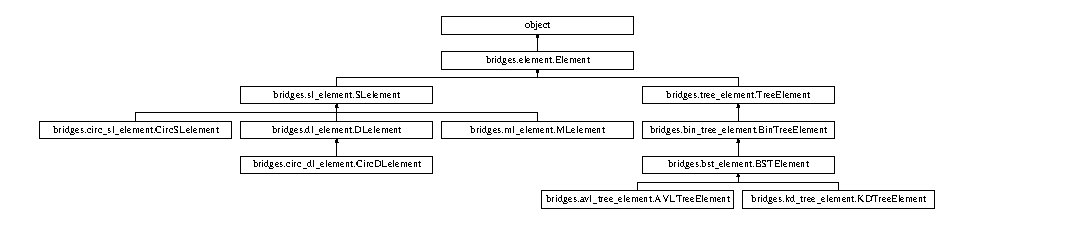
\includegraphics[height=2.145594cm]{classbridges_1_1element_1_1_element}
\end{center}
\end{figure}
\doxysubsection*{Public Member Functions}
\begin{DoxyCompactItemize}
\item 
str \mbox{\hyperlink{classbridges_1_1element_1_1_element_ada235252964d163ab1df8a9609b2af5b}{get\+\_\+data\+\_\+structure\+\_\+type}} (self)
\begin{DoxyCompactList}\small\item\em Get the data structure representation. \end{DoxyCompactList}\item 
None \mbox{\hyperlink{classbridges_1_1element_1_1_element_a59432b0af6594a2c8b57602eb8fc4906}{\+\_\+\+\_\+init\+\_\+\+\_\+}} (self, $\ast$$\ast$kwargs)
\begin{DoxyCompactList}\small\item\em \mbox{\hyperlink{classbridges_1_1element_1_1_element}{Element}} constructor. \end{DoxyCompactList}\item 
object \mbox{\hyperlink{classbridges_1_1element_1_1_element_ad18e8738e025d7af322144aecbec1629}{value}} (self)
\begin{DoxyCompactList}\small\item\em Getter for the value this element is holding. \end{DoxyCompactList}\item 
None \mbox{\hyperlink{classbridges_1_1element_1_1_element_ab2b6e30e1c3443ddde043b919e1d7ef5}{value}} (self, val)
\begin{DoxyCompactList}\small\item\em Setter for the value of an element. \end{DoxyCompactList}\item 
str \mbox{\hyperlink{classbridges_1_1element_1_1_element_a31cdf36f75fe34aebec85b95025cc732}{identifier}} (self)
\begin{DoxyCompactList}\small\item\em Getter for the element identifier. \end{DoxyCompactList}\item 
None \mbox{\hyperlink{classbridges_1_1element_1_1_element_acdba2c20daeb16c7e6ce1f4d7192e782}{identifier}} (self, int \mbox{\hyperlink{classbridges_1_1element_1_1_element_a9f6bae5e3c8eec5ee2b4c11232221d46}{id}})
\begin{DoxyCompactList}\small\item\em Setter for the element identifier. \end{DoxyCompactList}\item 
\mbox{\hyperlink{classbridges_1_1element__visualizer_1_1_element_visualizer}{Element\+Visualizer}} \mbox{\hyperlink{classbridges_1_1element_1_1_element_a704bd547988e01648f5b2d40896145e9}{visualizer}} (self)
\begin{DoxyCompactList}\small\item\em Getter for the element visualizer. \end{DoxyCompactList}\item 
None \mbox{\hyperlink{classbridges_1_1element_1_1_element_a147c45010c473395ee93368a8e3ac6dc}{visualizer}} (self, \mbox{\hyperlink{classbridges_1_1element__visualizer_1_1_element_visualizer}{Element\+Visualizer}} vis)
\begin{DoxyCompactList}\small\item\em Setter function for this element visualizer. \end{DoxyCompactList}\item 
\mbox{\hyperlink{classbridges_1_1link__visualizer_1_1_link_visualizer}{Link\+Visualizer}} \mbox{\hyperlink{classbridges_1_1element_1_1_element_aab7758342bad869596c0c7b58b601209}{get\+\_\+link\+\_\+visualizer}} (self, el)
\item 
None \mbox{\hyperlink{classbridges_1_1element_1_1_element_ae2dd2e2d88be1e89adec25166d421813}{set\+\_\+link\+\_\+visualizer}} (self, el)
\begin{DoxyCompactList}\small\item\em Setter for the link visualizer of this element. \end{DoxyCompactList}\item 
None \mbox{\hyperlink{classbridges_1_1element_1_1_element_a08a71fea8b2e6bb19eba8ea04d8dae4b}{remove\+\_\+link\+\_\+visualizer}} (self, el)
\begin{DoxyCompactList}\small\item\em Deleter function for the lik visualizer of this element. \end{DoxyCompactList}\item 
def \mbox{\hyperlink{classbridges_1_1element_1_1_element_a3cd2f535bb7993254b8d255cb0166062}{label}} (self)
\begin{DoxyCompactList}\small\item\em Getter for the element\textquotesingle{}s label. \end{DoxyCompactList}\item 
def \mbox{\hyperlink{classbridges_1_1element_1_1_element_a29dd33558e94464186658d2baad1d6c9}{label}} (self, label)
\begin{DoxyCompactList}\small\item\em Setter for the element\textquotesingle{}s label. \end{DoxyCompactList}\item 
def \mbox{\hyperlink{classbridges_1_1element_1_1_element_a4d25b09a11a282c8c8147b16cd45c5bf}{size}} (self)
\begin{DoxyCompactList}\small\item\em Getter for the element\textquotesingle{}s size. \end{DoxyCompactList}\item 
def \mbox{\hyperlink{classbridges_1_1element_1_1_element_afbb37ab4474c2ac1b7da950fb06819ed}{size}} (self, sz)
\begin{DoxyCompactList}\small\item\em Setter for the element\textquotesingle{}s size. \end{DoxyCompactList}\item 
def \mbox{\hyperlink{classbridges_1_1element_1_1_element_af8bf34079130638064db0b03ef5bb79a}{color}} (self)
\begin{DoxyCompactList}\small\item\em Getter for the element\textquotesingle{}s color. \end{DoxyCompactList}\item 
def \mbox{\hyperlink{classbridges_1_1element_1_1_element_ace59b1eb4cf0d775e9afa31605183c50}{color}} (self, col)
\begin{DoxyCompactList}\small\item\em Setter for the element\textquotesingle{}s size. \end{DoxyCompactList}\item 
def \mbox{\hyperlink{classbridges_1_1element_1_1_element_a31ce56c32bd400a2d8d0e7e146c4b5f3}{opacity}} (self)
\begin{DoxyCompactList}\small\item\em Getter for the element\textquotesingle{}s opacity. \end{DoxyCompactList}\item 
def \mbox{\hyperlink{classbridges_1_1element_1_1_element_a1542425770b360b39369e3db7116d6ae}{opacity}} (self, op)
\begin{DoxyCompactList}\small\item\em Setter for the element\textquotesingle{}s opacity. \end{DoxyCompactList}\item 
def \mbox{\hyperlink{classbridges_1_1element_1_1_element_a4485e4854639bcb163a36d0629f0e8f9}{shape}} (self)
\begin{DoxyCompactList}\small\item\em Getter for the element\textquotesingle{}s shape type. \end{DoxyCompactList}\item 
def \mbox{\hyperlink{classbridges_1_1element_1_1_element_a54d45aa4c09c0b5745cebbabcc0c02f9}{shape}} (self, shp)
\begin{DoxyCompactList}\small\item\em Setter for the element\textquotesingle{}s shape. \end{DoxyCompactList}\item 
int \mbox{\hyperlink{classbridges_1_1element_1_1_element_a9f6bae5e3c8eec5ee2b4c11232221d46}{id}} (self)
\begin{DoxyCompactList}\small\item\em Get numer of ids of element object. \end{DoxyCompactList}\item 
def \mbox{\hyperlink{classbridges_1_1element_1_1_element_aa1387621f7afa6b6f6acd052a1126320}{set\+\_\+location}} (self, locX, locY)
\begin{DoxyCompactList}\small\item\em Setter for the element\textquotesingle{}s location. \end{DoxyCompactList}\item 
def \mbox{\hyperlink{classbridges_1_1element_1_1_element_aa921953dab3cec5253e813bb1709895a}{get\+\_\+locationX}} (self)
\begin{DoxyCompactList}\small\item\em Getter for the element\textquotesingle{}s location in X. \end{DoxyCompactList}\item 
def \mbox{\hyperlink{classbridges_1_1element_1_1_element_a108f62843d084beaf5fcf5fd202853c5}{get\+\_\+locationY}} (self)
\begin{DoxyCompactList}\small\item\em Getter for the element\textquotesingle{}s location in Y. \end{DoxyCompactList}\item 
def \mbox{\hyperlink{classbridges_1_1element_1_1_element_a511fbc6323616d806ae0ae33010f4654}{get\+\_\+element\+\_\+representation}} (self)
\begin{DoxyCompactList}\small\item\em Getter for the element\textquotesingle{}s JSON representation (for internal use) \end{DoxyCompactList}\item 
def \mbox{\hyperlink{classbridges_1_1element_1_1_element_a8f220d7b81c0e0dd84b9eff33ade76b9}{get\+\_\+link\+\_\+representation}} (self, lv, src, dest)
\begin{DoxyCompactList}\small\item\em Getter for the JSON representation of the element\textquotesingle{}s link (for internal use) \end{DoxyCompactList}\end{DoxyCompactItemize}
\doxysubsection*{Public Attributes}
\begin{DoxyCompactItemize}
\item 
\mbox{\hyperlink{classbridges_1_1element_1_1_element_a568fd16a353d7852571aa947433095ea}{color}}
\item 
\mbox{\hyperlink{classbridges_1_1element_1_1_element_a5af50d5fc696eb8c295245bd5d1c0c91}{opacity}}
\end{DoxyCompactItemize}
\doxysubsection*{Static Public Attributes}
\begin{DoxyCompactItemize}
\item 
int \mbox{\hyperlink{classbridges_1_1element_1_1_element_a61f02c915a65554b76dd6534e5a4d834}{ids}} = 0
\end{DoxyCompactItemize}


\doxysubsection{Constructor \& Destructor Documentation}
\mbox{\Hypertarget{classbridges_1_1element_1_1_element_a59432b0af6594a2c8b57602eb8fc4906}\label{classbridges_1_1element_1_1_element_a59432b0af6594a2c8b57602eb8fc4906}} 
\index{bridges.element.Element@{bridges.element.Element}!\_\_init\_\_@{\_\_init\_\_}}
\index{\_\_init\_\_@{\_\_init\_\_}!bridges.element.Element@{bridges.element.Element}}
\doxysubsubsection{\texorpdfstring{\_\_init\_\_()}{\_\_init\_\_()}}
{\footnotesize\ttfamily  None bridges.\+element.\+Element.\+\_\+\+\_\+init\+\_\+\+\_\+ (\begin{DoxyParamCaption}\item[{}]{self,  }\item[{$\ast$$\ast$}]{kwargs }\end{DoxyParamCaption})}



\mbox{\hyperlink{classbridges_1_1element_1_1_element}{Element}} constructor. 

Creates an \mbox{\hyperlink{classbridges_1_1element_1_1_element}{Element}} Visualizer and unique identifier for the current element. \begin{DoxyVerb}       (0) : "label" - the string label that is visible on the bridges Visualization
       (1) : "value" - data value (or object) E  used to construct Element
       (2) : "original" - element object to copy (if named "original")
       (3) : "color"  - color of element
       (4) : "opacity" - opacity of element
\end{DoxyVerb}
 \begin{DoxyReturn}{Returns}


None 
\end{DoxyReturn}


Reimplemented in \mbox{\hyperlink{classbridges_1_1tree__element_1_1_tree_element_aec95cc1608f0c741ddd7e7a63174f3b7}{bridges.\+tree\+\_\+element.\+Tree\+Element}}, \mbox{\hyperlink{classbridges_1_1sl__element_1_1_s_lelement_a0824caaa305931953bf3f6d53d3a3d14}{bridges.\+sl\+\_\+element.\+SLelement}}, \mbox{\hyperlink{classbridges_1_1ml__element_1_1_m_lelement_abd5ccc3a5438e2ed1812be381f4fb8a4}{bridges.\+ml\+\_\+element.\+MLelement}}, \mbox{\hyperlink{classbridges_1_1kd__tree__element_1_1_k_d_tree_element_ad48f0bdabbb21cf83782efc1f8dbc1ed}{bridges.\+kd\+\_\+tree\+\_\+element.\+KDTree\+Element}}, \mbox{\hyperlink{classbridges_1_1circ__sl__element_1_1_circ_s_lelement_a3885ad93ae1368cfef8296ace0ab22c8}{bridges.\+circ\+\_\+sl\+\_\+element.\+Circ\+SLelement}}, \mbox{\hyperlink{classbridges_1_1circ__dl__element_1_1_circ_d_lelement_a6db1440877da650713f41a3450377d49}{bridges.\+circ\+\_\+dl\+\_\+element.\+Circ\+DLelement}}, \mbox{\hyperlink{classbridges_1_1bst__element_1_1_b_s_t_element_a0be9b75a1da9322d40811669d13e05a4}{bridges.\+bst\+\_\+element.\+BSTElement}}, and \mbox{\hyperlink{classbridges_1_1bin__tree__element_1_1_bin_tree_element_a4c50812c9a43aa5cd75ccc46b818a8b2}{bridges.\+bin\+\_\+tree\+\_\+element.\+Bin\+Tree\+Element}}.



\doxysubsection{Member Function Documentation}
\mbox{\Hypertarget{classbridges_1_1element_1_1_element_af8bf34079130638064db0b03ef5bb79a}\label{classbridges_1_1element_1_1_element_af8bf34079130638064db0b03ef5bb79a}} 
\index{bridges.element.Element@{bridges.element.Element}!color@{color}}
\index{color@{color}!bridges.element.Element@{bridges.element.Element}}
\doxysubsubsection{\texorpdfstring{color()}{color()}\hspace{0.1cm}{\footnotesize\ttfamily [1/2]}}
{\footnotesize\ttfamily def bridges.\+element.\+Element.\+color (\begin{DoxyParamCaption}\item[{}]{self }\end{DoxyParamCaption})}



Getter for the element\textquotesingle{}s color. 

\begin{DoxyReturn}{Returns}


Color element\textquotesingle{}s color 
\end{DoxyReturn}
\mbox{\Hypertarget{classbridges_1_1element_1_1_element_ace59b1eb4cf0d775e9afa31605183c50}\label{classbridges_1_1element_1_1_element_ace59b1eb4cf0d775e9afa31605183c50}} 
\index{bridges.element.Element@{bridges.element.Element}!color@{color}}
\index{color@{color}!bridges.element.Element@{bridges.element.Element}}
\doxysubsubsection{\texorpdfstring{color()}{color()}\hspace{0.1cm}{\footnotesize\ttfamily [2/2]}}
{\footnotesize\ttfamily def bridges.\+element.\+Element.\+color (\begin{DoxyParamCaption}\item[{}]{self,  }\item[{}]{col }\end{DoxyParamCaption})}



Setter for the element\textquotesingle{}s size. 


\begin{DoxyParams}{Parameters}
{\em col} & the element\textquotesingle{}s color \\
\hline
\end{DoxyParams}
\begin{DoxyReturn}{Returns}


None 
\end{DoxyReturn}
\mbox{\Hypertarget{classbridges_1_1element_1_1_element_ada235252964d163ab1df8a9609b2af5b}\label{classbridges_1_1element_1_1_element_ada235252964d163ab1df8a9609b2af5b}} 
\index{bridges.element.Element@{bridges.element.Element}!get\_data\_structure\_type@{get\_data\_structure\_type}}
\index{get\_data\_structure\_type@{get\_data\_structure\_type}!bridges.element.Element@{bridges.element.Element}}
\doxysubsubsection{\texorpdfstring{get\_data\_structure\_type()}{get\_data\_structure\_type()}}
{\footnotesize\ttfamily  str bridges.\+element.\+Element.\+get\+\_\+data\+\_\+structure\+\_\+type (\begin{DoxyParamCaption}\item[{}]{self }\end{DoxyParamCaption})}



Get the data structure representation. 

\begin{DoxyReturn}{Returns}


str representing the data structure type 
\end{DoxyReturn}


Reimplemented in \mbox{\hyperlink{classbridges_1_1tree__element_1_1_tree_element_a54a14bd74fe1f86dd73f90c57f88c10b}{bridges.\+tree\+\_\+element.\+Tree\+Element}}, \mbox{\hyperlink{classbridges_1_1sl__element_1_1_s_lelement_ae6d1c0479d0ed763e1ea54f5d2f9a0eb}{bridges.\+sl\+\_\+element.\+SLelement}}, \mbox{\hyperlink{classbridges_1_1ml__element_1_1_m_lelement_a756749f461e226ce7ae7e46f6efa48f8}{bridges.\+ml\+\_\+element.\+MLelement}}, \mbox{\hyperlink{classbridges_1_1kd__tree__element_1_1_k_d_tree_element_a4b38af960542ccc8c3b74d90ee9570e2}{bridges.\+kd\+\_\+tree\+\_\+element.\+KDTree\+Element}}, \mbox{\hyperlink{classbridges_1_1dl__element_1_1_d_lelement_a6ffddb5ac79a3945c1559dbc2236ab81}{bridges.\+dl\+\_\+element.\+DLelement}}, \mbox{\hyperlink{classbridges_1_1circ__sl__element_1_1_circ_s_lelement_a417f0fa7de0f4d1017ca7a27870c45d3}{bridges.\+circ\+\_\+sl\+\_\+element.\+Circ\+SLelement}}, \mbox{\hyperlink{classbridges_1_1circ__dl__element_1_1_circ_d_lelement_a86837fc443104b20589874000821afbd}{bridges.\+circ\+\_\+dl\+\_\+element.\+Circ\+DLelement}}, \mbox{\hyperlink{classbridges_1_1bst__element_1_1_b_s_t_element_a8e655e06ba0f77b7e2681b6d291f39de}{bridges.\+bst\+\_\+element.\+BSTElement}}, \mbox{\hyperlink{classbridges_1_1bin__tree__element_1_1_bin_tree_element_a9238744e18486fb8882238394f5efe7c}{bridges.\+bin\+\_\+tree\+\_\+element.\+Bin\+Tree\+Element}}, and \mbox{\hyperlink{classbridges_1_1avl__tree__element_1_1_a_v_l_tree_element_a811dd4cebd36fda6531f6cbeb873c0e5}{bridges.\+avl\+\_\+tree\+\_\+element.\+AVLTree\+Element}}.

\mbox{\Hypertarget{classbridges_1_1element_1_1_element_a511fbc6323616d806ae0ae33010f4654}\label{classbridges_1_1element_1_1_element_a511fbc6323616d806ae0ae33010f4654}} 
\index{bridges.element.Element@{bridges.element.Element}!get\_element\_representation@{get\_element\_representation}}
\index{get\_element\_representation@{get\_element\_representation}!bridges.element.Element@{bridges.element.Element}}
\doxysubsubsection{\texorpdfstring{get\_element\_representation()}{get\_element\_representation()}}
{\footnotesize\ttfamily def bridges.\+element.\+Element.\+get\+\_\+element\+\_\+representation (\begin{DoxyParamCaption}\item[{}]{self }\end{DoxyParamCaption})}



Getter for the element\textquotesingle{}s JSON representation (for internal use) 

\begin{DoxyReturn}{Returns}


str JSON of element 
\end{DoxyReturn}


Reimplemented in \mbox{\hyperlink{classbridges_1_1kd__tree__element_1_1_k_d_tree_element_a4e08a6f2e4ff70be2b0dfd6eacdcf10e}{bridges.\+kd\+\_\+tree\+\_\+element.\+KDTree\+Element}}, \mbox{\hyperlink{classbridges_1_1bst__element_1_1_b_s_t_element_a9d038f191a7cf06e75910463a3aa3b80}{bridges.\+bst\+\_\+element.\+BSTElement}}, and \mbox{\hyperlink{classbridges_1_1avl__tree__element_1_1_a_v_l_tree_element_abf8842cb462f1e31f0889d67fb0d70d4}{bridges.\+avl\+\_\+tree\+\_\+element.\+AVLTree\+Element}}.

\mbox{\Hypertarget{classbridges_1_1element_1_1_element_a8f220d7b81c0e0dd84b9eff33ade76b9}\label{classbridges_1_1element_1_1_element_a8f220d7b81c0e0dd84b9eff33ade76b9}} 
\index{bridges.element.Element@{bridges.element.Element}!get\_link\_representation@{get\_link\_representation}}
\index{get\_link\_representation@{get\_link\_representation}!bridges.element.Element@{bridges.element.Element}}
\doxysubsubsection{\texorpdfstring{get\_link\_representation()}{get\_link\_representation()}}
{\footnotesize\ttfamily def bridges.\+element.\+Element.\+get\+\_\+link\+\_\+representation (\begin{DoxyParamCaption}\item[{}]{self,  }\item[{}]{lv,  }\item[{}]{src,  }\item[{}]{dest }\end{DoxyParamCaption})}



Getter for the JSON representation of the element\textquotesingle{}s link (for internal use) 


\begin{DoxyParams}{Parameters}
{\em lv} & link visualizer \\
\hline
{\em src} & source vertex of link \\
\hline
{\em dest} & destination vertex of link \\
\hline
\end{DoxyParams}
\begin{DoxyReturn}{Returns}


str JSON of element\textquotesingle{}s link from src to dest 
\end{DoxyReturn}
\mbox{\Hypertarget{classbridges_1_1element_1_1_element_aab7758342bad869596c0c7b58b601209}\label{classbridges_1_1element_1_1_element_aab7758342bad869596c0c7b58b601209}} 
\index{bridges.element.Element@{bridges.element.Element}!get\_link\_visualizer@{get\_link\_visualizer}}
\index{get\_link\_visualizer@{get\_link\_visualizer}!bridges.element.Element@{bridges.element.Element}}
\doxysubsubsection{\texorpdfstring{get\_link\_visualizer()}{get\_link\_visualizer()}}
{\footnotesize\ttfamily  \mbox{\hyperlink{classbridges_1_1link__visualizer_1_1_link_visualizer}{Link\+Visualizer}} bridges.\+element.\+Element.\+get\+\_\+link\+\_\+visualizer (\begin{DoxyParamCaption}\item[{}]{self,  }\item[{}]{el }\end{DoxyParamCaption})}

\mbox{\Hypertarget{classbridges_1_1element_1_1_element_aa921953dab3cec5253e813bb1709895a}\label{classbridges_1_1element_1_1_element_aa921953dab3cec5253e813bb1709895a}} 
\index{bridges.element.Element@{bridges.element.Element}!get\_locationX@{get\_locationX}}
\index{get\_locationX@{get\_locationX}!bridges.element.Element@{bridges.element.Element}}
\doxysubsubsection{\texorpdfstring{get\_locationX()}{get\_locationX()}}
{\footnotesize\ttfamily def bridges.\+element.\+Element.\+get\+\_\+locationX (\begin{DoxyParamCaption}\item[{}]{self }\end{DoxyParamCaption})}



Getter for the element\textquotesingle{}s location in X. 

\begin{DoxyReturn}{Returns}


float X coordinate of element\textquotesingle{}s location 
\end{DoxyReturn}
\mbox{\Hypertarget{classbridges_1_1element_1_1_element_a108f62843d084beaf5fcf5fd202853c5}\label{classbridges_1_1element_1_1_element_a108f62843d084beaf5fcf5fd202853c5}} 
\index{bridges.element.Element@{bridges.element.Element}!get\_locationY@{get\_locationY}}
\index{get\_locationY@{get\_locationY}!bridges.element.Element@{bridges.element.Element}}
\doxysubsubsection{\texorpdfstring{get\_locationY()}{get\_locationY()}}
{\footnotesize\ttfamily def bridges.\+element.\+Element.\+get\+\_\+locationY (\begin{DoxyParamCaption}\item[{}]{self }\end{DoxyParamCaption})}



Getter for the element\textquotesingle{}s location in Y. 

\begin{DoxyReturn}{Returns}


float Y coordinate of element\textquotesingle{}s location 
\end{DoxyReturn}
\mbox{\Hypertarget{classbridges_1_1element_1_1_element_a9f6bae5e3c8eec5ee2b4c11232221d46}\label{classbridges_1_1element_1_1_element_a9f6bae5e3c8eec5ee2b4c11232221d46}} 
\index{bridges.element.Element@{bridges.element.Element}!id@{id}}
\index{id@{id}!bridges.element.Element@{bridges.element.Element}}
\doxysubsubsection{\texorpdfstring{id()}{id()}}
{\footnotesize\ttfamily  int bridges.\+element.\+Element.\+id (\begin{DoxyParamCaption}\item[{}]{self }\end{DoxyParamCaption})}



Get numer of ids of element object. 

\begin{DoxyReturn}{Returns}
(int) number of ids of element 
\end{DoxyReturn}
\mbox{\Hypertarget{classbridges_1_1element_1_1_element_a31cdf36f75fe34aebec85b95025cc732}\label{classbridges_1_1element_1_1_element_a31cdf36f75fe34aebec85b95025cc732}} 
\index{bridges.element.Element@{bridges.element.Element}!identifier@{identifier}}
\index{identifier@{identifier}!bridges.element.Element@{bridges.element.Element}}
\doxysubsubsection{\texorpdfstring{identifier()}{identifier()}\hspace{0.1cm}{\footnotesize\ttfamily [1/2]}}
{\footnotesize\ttfamily  str bridges.\+element.\+Element.\+identifier (\begin{DoxyParamCaption}\item[{}]{self }\end{DoxyParamCaption})}



Getter for the element identifier. 

\begin{DoxyParagraph}{Return}
str element identifier (for internal use) 
\end{DoxyParagraph}
\mbox{\Hypertarget{classbridges_1_1element_1_1_element_acdba2c20daeb16c7e6ce1f4d7192e782}\label{classbridges_1_1element_1_1_element_acdba2c20daeb16c7e6ce1f4d7192e782}} 
\index{bridges.element.Element@{bridges.element.Element}!identifier@{identifier}}
\index{identifier@{identifier}!bridges.element.Element@{bridges.element.Element}}
\doxysubsubsection{\texorpdfstring{identifier()}{identifier()}\hspace{0.1cm}{\footnotesize\ttfamily [2/2]}}
{\footnotesize\ttfamily  None bridges.\+element.\+Element.\+identifier (\begin{DoxyParamCaption}\item[{}]{self,  }\item[{int}]{id }\end{DoxyParamCaption})}



Setter for the element identifier. 


\begin{DoxyParams}{Parameters}
{\em id} & the identifier (for internal use) \\
\hline
\end{DoxyParams}
\begin{DoxyReturn}{Returns}


None 
\end{DoxyReturn}
\mbox{\Hypertarget{classbridges_1_1element_1_1_element_a3cd2f535bb7993254b8d255cb0166062}\label{classbridges_1_1element_1_1_element_a3cd2f535bb7993254b8d255cb0166062}} 
\index{bridges.element.Element@{bridges.element.Element}!label@{label}}
\index{label@{label}!bridges.element.Element@{bridges.element.Element}}
\doxysubsubsection{\texorpdfstring{label()}{label()}\hspace{0.1cm}{\footnotesize\ttfamily [1/2]}}
{\footnotesize\ttfamily def bridges.\+element.\+Element.\+label (\begin{DoxyParamCaption}\item[{}]{self }\end{DoxyParamCaption})}



Getter for the element\textquotesingle{}s label. 

\begin{DoxyReturn}{Returns}


str the element\textquotesingle{}s label 
\end{DoxyReturn}
\mbox{\Hypertarget{classbridges_1_1element_1_1_element_a29dd33558e94464186658d2baad1d6c9}\label{classbridges_1_1element_1_1_element_a29dd33558e94464186658d2baad1d6c9}} 
\index{bridges.element.Element@{bridges.element.Element}!label@{label}}
\index{label@{label}!bridges.element.Element@{bridges.element.Element}}
\doxysubsubsection{\texorpdfstring{label()}{label()}\hspace{0.1cm}{\footnotesize\ttfamily [2/2]}}
{\footnotesize\ttfamily def bridges.\+element.\+Element.\+label (\begin{DoxyParamCaption}\item[{}]{self,  }\item[{}]{label }\end{DoxyParamCaption})}



Setter for the element\textquotesingle{}s label. 


\begin{DoxyParams}{Parameters}
{\em label} & the element\textquotesingle{}s label \\
\hline
\end{DoxyParams}
\begin{DoxyReturn}{Returns}


None 
\end{DoxyReturn}
\mbox{\Hypertarget{classbridges_1_1element_1_1_element_a31ce56c32bd400a2d8d0e7e146c4b5f3}\label{classbridges_1_1element_1_1_element_a31ce56c32bd400a2d8d0e7e146c4b5f3}} 
\index{bridges.element.Element@{bridges.element.Element}!opacity@{opacity}}
\index{opacity@{opacity}!bridges.element.Element@{bridges.element.Element}}
\doxysubsubsection{\texorpdfstring{opacity()}{opacity()}\hspace{0.1cm}{\footnotesize\ttfamily [1/2]}}
{\footnotesize\ttfamily def bridges.\+element.\+Element.\+opacity (\begin{DoxyParamCaption}\item[{}]{self }\end{DoxyParamCaption})}



Getter for the element\textquotesingle{}s opacity. 

\begin{DoxyReturn}{Returns}


float element size (0-\/1.\+0) 
\end{DoxyReturn}
\mbox{\Hypertarget{classbridges_1_1element_1_1_element_a1542425770b360b39369e3db7116d6ae}\label{classbridges_1_1element_1_1_element_a1542425770b360b39369e3db7116d6ae}} 
\index{bridges.element.Element@{bridges.element.Element}!opacity@{opacity}}
\index{opacity@{opacity}!bridges.element.Element@{bridges.element.Element}}
\doxysubsubsection{\texorpdfstring{opacity()}{opacity()}\hspace{0.1cm}{\footnotesize\ttfamily [2/2]}}
{\footnotesize\ttfamily def bridges.\+element.\+Element.\+opacity (\begin{DoxyParamCaption}\item[{}]{self,  }\item[{}]{op }\end{DoxyParamCaption})}



Setter for the element\textquotesingle{}s opacity. 


\begin{DoxyParams}{Parameters}
{\em op} & the element\textquotesingle{}s size (0-\/1.\+0) \\
\hline
\end{DoxyParams}
\begin{DoxyReturn}{Returns}


None 
\end{DoxyReturn}
\mbox{\Hypertarget{classbridges_1_1element_1_1_element_a08a71fea8b2e6bb19eba8ea04d8dae4b}\label{classbridges_1_1element_1_1_element_a08a71fea8b2e6bb19eba8ea04d8dae4b}} 
\index{bridges.element.Element@{bridges.element.Element}!remove\_link\_visualizer@{remove\_link\_visualizer}}
\index{remove\_link\_visualizer@{remove\_link\_visualizer}!bridges.element.Element@{bridges.element.Element}}
\doxysubsubsection{\texorpdfstring{remove\_link\_visualizer()}{remove\_link\_visualizer()}}
{\footnotesize\ttfamily  None bridges.\+element.\+Element.\+remove\+\_\+link\+\_\+visualizer (\begin{DoxyParamCaption}\item[{}]{self,  }\item[{}]{el }\end{DoxyParamCaption})}



Deleter function for the lik visualizer of this element. 

\begin{DoxyVerb}       (Element) el: the terminating element of the link; the link visualizer
       for this link will be deleted
\end{DoxyVerb}
 \begin{DoxyReturn}{Returns}


None 
\end{DoxyReturn}
\mbox{\Hypertarget{classbridges_1_1element_1_1_element_ae2dd2e2d88be1e89adec25166d421813}\label{classbridges_1_1element_1_1_element_ae2dd2e2d88be1e89adec25166d421813}} 
\index{bridges.element.Element@{bridges.element.Element}!set\_link\_visualizer@{set\_link\_visualizer}}
\index{set\_link\_visualizer@{set\_link\_visualizer}!bridges.element.Element@{bridges.element.Element}}
\doxysubsubsection{\texorpdfstring{set\_link\_visualizer()}{set\_link\_visualizer()}}
{\footnotesize\ttfamily  None bridges.\+element.\+Element.\+set\+\_\+link\+\_\+visualizer (\begin{DoxyParamCaption}\item[{}]{self,  }\item[{}]{el }\end{DoxyParamCaption})}



Setter for the link visualizer of this element. 

\begin{DoxyVerb}       (Element) el: the terminating element of this link;
        creates a new link visualizer for this link
\end{DoxyVerb}
 \begin{DoxyReturn}{Returns}


None 
\end{DoxyReturn}
\mbox{\Hypertarget{classbridges_1_1element_1_1_element_aa1387621f7afa6b6f6acd052a1126320}\label{classbridges_1_1element_1_1_element_aa1387621f7afa6b6f6acd052a1126320}} 
\index{bridges.element.Element@{bridges.element.Element}!set\_location@{set\_location}}
\index{set\_location@{set\_location}!bridges.element.Element@{bridges.element.Element}}
\doxysubsubsection{\texorpdfstring{set\_location()}{set\_location()}}
{\footnotesize\ttfamily def bridges.\+element.\+Element.\+set\+\_\+location (\begin{DoxyParamCaption}\item[{}]{self,  }\item[{}]{locX,  }\item[{}]{locY }\end{DoxyParamCaption})}



Setter for the element\textquotesingle{}s location. 


\begin{DoxyParams}{Parameters}
{\em locX} & the element\textquotesingle{}s location in X \\
\hline
{\em locY} & the element\textquotesingle{}s location in Y \\
\hline
\end{DoxyParams}
\begin{DoxyReturn}{Returns}


None 
\end{DoxyReturn}
\mbox{\Hypertarget{classbridges_1_1element_1_1_element_a4485e4854639bcb163a36d0629f0e8f9}\label{classbridges_1_1element_1_1_element_a4485e4854639bcb163a36d0629f0e8f9}} 
\index{bridges.element.Element@{bridges.element.Element}!shape@{shape}}
\index{shape@{shape}!bridges.element.Element@{bridges.element.Element}}
\doxysubsubsection{\texorpdfstring{shape()}{shape()}\hspace{0.1cm}{\footnotesize\ttfamily [1/2]}}
{\footnotesize\ttfamily def bridges.\+element.\+Element.\+shape (\begin{DoxyParamCaption}\item[{}]{self }\end{DoxyParamCaption})}



Getter for the element\textquotesingle{}s shape type. 

\begin{DoxyReturn}{Returns}
element shape 
\end{DoxyReturn}
\mbox{\Hypertarget{classbridges_1_1element_1_1_element_a54d45aa4c09c0b5745cebbabcc0c02f9}\label{classbridges_1_1element_1_1_element_a54d45aa4c09c0b5745cebbabcc0c02f9}} 
\index{bridges.element.Element@{bridges.element.Element}!shape@{shape}}
\index{shape@{shape}!bridges.element.Element@{bridges.element.Element}}
\doxysubsubsection{\texorpdfstring{shape()}{shape()}\hspace{0.1cm}{\footnotesize\ttfamily [2/2]}}
{\footnotesize\ttfamily def bridges.\+element.\+Element.\+shape (\begin{DoxyParamCaption}\item[{}]{self,  }\item[{}]{shp }\end{DoxyParamCaption})}



Setter for the element\textquotesingle{}s shape. 


\begin{DoxyParams}{Parameters}
{\em shp} & the element\textquotesingle{}s size (0-\/1.\+0) \\
\hline
\end{DoxyParams}
\begin{DoxyReturn}{Returns}


None 
\end{DoxyReturn}
\mbox{\Hypertarget{classbridges_1_1element_1_1_element_a4d25b09a11a282c8c8147b16cd45c5bf}\label{classbridges_1_1element_1_1_element_a4d25b09a11a282c8c8147b16cd45c5bf}} 
\index{bridges.element.Element@{bridges.element.Element}!size@{size}}
\index{size@{size}!bridges.element.Element@{bridges.element.Element}}
\doxysubsubsection{\texorpdfstring{size()}{size()}\hspace{0.1cm}{\footnotesize\ttfamily [1/2]}}
{\footnotesize\ttfamily def bridges.\+element.\+Element.\+size (\begin{DoxyParamCaption}\item[{}]{self }\end{DoxyParamCaption})}



Getter for the element\textquotesingle{}s size. 

\begin{DoxyReturn}{Returns}


float element size (0-\/50) 
\end{DoxyReturn}
\mbox{\Hypertarget{classbridges_1_1element_1_1_element_afbb37ab4474c2ac1b7da950fb06819ed}\label{classbridges_1_1element_1_1_element_afbb37ab4474c2ac1b7da950fb06819ed}} 
\index{bridges.element.Element@{bridges.element.Element}!size@{size}}
\index{size@{size}!bridges.element.Element@{bridges.element.Element}}
\doxysubsubsection{\texorpdfstring{size()}{size()}\hspace{0.1cm}{\footnotesize\ttfamily [2/2]}}
{\footnotesize\ttfamily def bridges.\+element.\+Element.\+size (\begin{DoxyParamCaption}\item[{}]{self,  }\item[{}]{sz }\end{DoxyParamCaption})}



Setter for the element\textquotesingle{}s size. 


\begin{DoxyParams}{Parameters}
{\em sz} & the element\textquotesingle{}s size (0.-\/50.) \\
\hline
\end{DoxyParams}
\begin{DoxyReturn}{Returns}


None 
\end{DoxyReturn}
\mbox{\Hypertarget{classbridges_1_1element_1_1_element_ad18e8738e025d7af322144aecbec1629}\label{classbridges_1_1element_1_1_element_ad18e8738e025d7af322144aecbec1629}} 
\index{bridges.element.Element@{bridges.element.Element}!value@{value}}
\index{value@{value}!bridges.element.Element@{bridges.element.Element}}
\doxysubsubsection{\texorpdfstring{value()}{value()}\hspace{0.1cm}{\footnotesize\ttfamily [1/2]}}
{\footnotesize\ttfamily  object bridges.\+element.\+Element.\+value (\begin{DoxyParamCaption}\item[{}]{self }\end{DoxyParamCaption})}



Getter for the value this element is holding. 

\begin{DoxyReturn}{Returns}
generic object (application specific) 
\end{DoxyReturn}


Reimplemented in \mbox{\hyperlink{classbridges_1_1sl__element_1_1_s_lelement_a64ede02c56a4efaaa4c64a245bd01dd0}{bridges.\+sl\+\_\+element.\+SLelement}}.

\mbox{\Hypertarget{classbridges_1_1element_1_1_element_ab2b6e30e1c3443ddde043b919e1d7ef5}\label{classbridges_1_1element_1_1_element_ab2b6e30e1c3443ddde043b919e1d7ef5}} 
\index{bridges.element.Element@{bridges.element.Element}!value@{value}}
\index{value@{value}!bridges.element.Element@{bridges.element.Element}}
\doxysubsubsection{\texorpdfstring{value()}{value()}\hspace{0.1cm}{\footnotesize\ttfamily [2/2]}}
{\footnotesize\ttfamily  None bridges.\+element.\+Element.\+value (\begin{DoxyParamCaption}\item[{}]{self,  }\item[{}]{val }\end{DoxyParamCaption})}



Setter for the value of an element. 


\begin{DoxyParams}{Parameters}
{\em val} & the value (generic, application specific object) this element will hold \\
\hline
\end{DoxyParams}
\begin{DoxyReturn}{Returns}


None 
\end{DoxyReturn}


Reimplemented in \mbox{\hyperlink{classbridges_1_1sl__element_1_1_s_lelement_a7653b41a8bc2c8ba7a71f07c8b0b8f3f}{bridges.\+sl\+\_\+element.\+SLelement}}.

\mbox{\Hypertarget{classbridges_1_1element_1_1_element_a704bd547988e01648f5b2d40896145e9}\label{classbridges_1_1element_1_1_element_a704bd547988e01648f5b2d40896145e9}} 
\index{bridges.element.Element@{bridges.element.Element}!visualizer@{visualizer}}
\index{visualizer@{visualizer}!bridges.element.Element@{bridges.element.Element}}
\doxysubsubsection{\texorpdfstring{visualizer()}{visualizer()}\hspace{0.1cm}{\footnotesize\ttfamily [1/2]}}
{\footnotesize\ttfamily  \mbox{\hyperlink{classbridges_1_1element__visualizer_1_1_element_visualizer}{Element\+Visualizer}} bridges.\+element.\+Element.\+visualizer (\begin{DoxyParamCaption}\item[{}]{self }\end{DoxyParamCaption})}



Getter for the element visualizer. 

\begin{DoxyReturn}{Returns}


Element\+Visualizer 
\end{DoxyReturn}
\mbox{\Hypertarget{classbridges_1_1element_1_1_element_a147c45010c473395ee93368a8e3ac6dc}\label{classbridges_1_1element_1_1_element_a147c45010c473395ee93368a8e3ac6dc}} 
\index{bridges.element.Element@{bridges.element.Element}!visualizer@{visualizer}}
\index{visualizer@{visualizer}!bridges.element.Element@{bridges.element.Element}}
\doxysubsubsection{\texorpdfstring{visualizer()}{visualizer()}\hspace{0.1cm}{\footnotesize\ttfamily [2/2]}}
{\footnotesize\ttfamily  None bridges.\+element.\+Element.\+visualizer (\begin{DoxyParamCaption}\item[{}]{self,  }\item[{\mbox{\hyperlink{classbridges_1_1element__visualizer_1_1_element_visualizer}{Element\+Visualizer}}}]{vis }\end{DoxyParamCaption})}



Setter function for this element visualizer. 


\begin{DoxyParams}{Parameters}
{\em vis} & the element visualizer \\
\hline
\end{DoxyParams}
\begin{DoxyReturn}{Returns}


None 
\end{DoxyReturn}


\doxysubsection{Member Data Documentation}
\mbox{\Hypertarget{classbridges_1_1element_1_1_element_a568fd16a353d7852571aa947433095ea}\label{classbridges_1_1element_1_1_element_a568fd16a353d7852571aa947433095ea}} 
\index{bridges.element.Element@{bridges.element.Element}!color@{color}}
\index{color@{color}!bridges.element.Element@{bridges.element.Element}}
\doxysubsubsection{\texorpdfstring{color}{color}}
{\footnotesize\ttfamily bridges.\+element.\+Element.\+color}

\mbox{\Hypertarget{classbridges_1_1element_1_1_element_a61f02c915a65554b76dd6534e5a4d834}\label{classbridges_1_1element_1_1_element_a61f02c915a65554b76dd6534e5a4d834}} 
\index{bridges.element.Element@{bridges.element.Element}!ids@{ids}}
\index{ids@{ids}!bridges.element.Element@{bridges.element.Element}}
\doxysubsubsection{\texorpdfstring{ids}{ids}}
{\footnotesize\ttfamily int bridges.\+element.\+Element.\+ids = 0\hspace{0.3cm}{\ttfamily [static]}}

\mbox{\Hypertarget{classbridges_1_1element_1_1_element_a5af50d5fc696eb8c295245bd5d1c0c91}\label{classbridges_1_1element_1_1_element_a5af50d5fc696eb8c295245bd5d1c0c91}} 
\index{bridges.element.Element@{bridges.element.Element}!opacity@{opacity}}
\index{opacity@{opacity}!bridges.element.Element@{bridges.element.Element}}
\doxysubsubsection{\texorpdfstring{opacity}{opacity}}
{\footnotesize\ttfamily bridges.\+element.\+Element.\+opacity}



The documentation for this class was generated from the following file\+:\begin{DoxyCompactItemize}
\item 
/\+Users/kalpathi/gr/bridges/client/python/bridges/\mbox{\hyperlink{element_8py}{element.\+py}}\end{DoxyCompactItemize}

\hypertarget{classbridges_1_1element__visualizer_1_1_element_visualizer}{}\doxysection{bridges.\+element\+\_\+visualizer.\+Element\+Visualizer Class Reference}
\label{classbridges_1_1element__visualizer_1_1_element_visualizer}\index{bridges.element\_visualizer.ElementVisualizer@{bridges.element\_visualizer.ElementVisualizer}}
\doxysubsection*{Public Member Functions}
\begin{DoxyCompactItemize}
\item 
def \mbox{\hyperlink{classbridges_1_1element__visualizer_1_1_element_visualizer_a27ee5eddf78bac93e2702b2f2203518a}{\+\_\+\+\_\+init\+\_\+\+\_\+}} (self, \mbox{\hyperlink{classbridges_1_1element__visualizer_1_1_element_visualizer_a1fd985698e1c56289ed49fa7849d43ab}{color}}=\char`\"{}green\char`\"{}, shape=\char`\"{}circle\char`\"{}, size=10.\+0, \mbox{\hyperlink{classbridges_1_1element__visualizer_1_1_element_visualizer_aaa4463337cf50610f4ee230bcdf2e483}{opacity}}=1.\+0)
\begin{DoxyCompactList}\small\item\em \mbox{\hyperlink{classbridges_1_1element__visualizer_1_1_element_visualizer}{Element\+Visualizer}} constuctor. \end{DoxyCompactList}\item 
float \mbox{\hyperlink{classbridges_1_1element__visualizer_1_1_element_visualizer_a4719523d913d90fc35aaa96bea674e65}{size}} (self)
\begin{DoxyCompactList}\small\item\em Getter for the elements size. \end{DoxyCompactList}\item 
None \mbox{\hyperlink{classbridges_1_1element__visualizer_1_1_element_visualizer_aa169210ab46d09ede9789910b844dd9e}{size}} (self, size)
\begin{DoxyCompactList}\small\item\em Setter for the size of the element. \end{DoxyCompactList}\item 
\mbox{\hyperlink{classbridges_1_1color_1_1_color}{Color}} \mbox{\hyperlink{classbridges_1_1element__visualizer_1_1_element_visualizer_a87d713b84157c9cb59d3185d9e364e17}{color}} (self)
\begin{DoxyCompactList}\small\item\em Getter for the color of the element in the bridges visualization. \end{DoxyCompactList}\item 
None \mbox{\hyperlink{classbridges_1_1element__visualizer_1_1_element_visualizer_a07fe381e92e2a62c7e62c425189d790e}{color}} (self, $\ast$args, $\ast$$\ast$kwargs)
\begin{DoxyCompactList}\small\item\em Setter for the color of the element in the bridges visualization. \end{DoxyCompactList}\item 
str \mbox{\hyperlink{classbridges_1_1element__visualizer_1_1_element_visualizer_a1a776963fc8564f010767457d5ea9118}{shape}} (self)
\begin{DoxyCompactList}\small\item\em Getter for the shape of the element. \end{DoxyCompactList}\item 
def \mbox{\hyperlink{classbridges_1_1element__visualizer_1_1_element_visualizer_af4bd377b8fb9a35c10740de7ea8c5eee}{shape}} (self, a\+\_\+shape)
\begin{DoxyCompactList}\small\item\em Setter for the shape of the element. \end{DoxyCompactList}\item 
float \mbox{\hyperlink{classbridges_1_1element__visualizer_1_1_element_visualizer_aaa4463337cf50610f4ee230bcdf2e483}{opacity}} (self)
\begin{DoxyCompactList}\small\item\em Getter for the opacity of the element. \end{DoxyCompactList}\item 
None \mbox{\hyperlink{classbridges_1_1element__visualizer_1_1_element_visualizer_ab0fe9377e980e9226e10177036a8d1cf}{opacity}} (self, opacity)
\begin{DoxyCompactList}\small\item\em Setter for the opacity of the element. \end{DoxyCompactList}\item 
def \mbox{\hyperlink{classbridges_1_1element__visualizer_1_1_element_visualizer_a7aef4402f2de7e88a3260bbec3a708a7}{set\+\_\+location}} (self, x, y)
\begin{DoxyCompactList}\small\item\em Setter for the location of the element. \end{DoxyCompactList}\item 
def \mbox{\hyperlink{classbridges_1_1element__visualizer_1_1_element_visualizer_a10fc24a04e43afcb393f3444bd93f5d9}{location\+\_\+x}} (self)
\begin{DoxyCompactList}\small\item\em Getter for the X location of element. \end{DoxyCompactList}\item 
def \mbox{\hyperlink{classbridges_1_1element__visualizer_1_1_element_visualizer_a687747f04ae17dea9d15706602688a32}{location\+\_\+y}} (self)
\begin{DoxyCompactList}\small\item\em Getter for the y location of the element. \end{DoxyCompactList}\end{DoxyCompactItemize}
\doxysubsection*{Public Attributes}
\begin{DoxyCompactItemize}
\item 
\mbox{\hyperlink{classbridges_1_1element__visualizer_1_1_element_visualizer_ac60ae1b3b3668b03dc4017e0ba4a199b}{prop}}
\item 
\mbox{\hyperlink{classbridges_1_1element__visualizer_1_1_element_visualizer_a1fd985698e1c56289ed49fa7849d43ab}{color}}
\end{DoxyCompactItemize}


\doxysubsection{Constructor \& Destructor Documentation}
\mbox{\Hypertarget{classbridges_1_1element__visualizer_1_1_element_visualizer_a27ee5eddf78bac93e2702b2f2203518a}\label{classbridges_1_1element__visualizer_1_1_element_visualizer_a27ee5eddf78bac93e2702b2f2203518a}} 
\index{bridges.element\_visualizer.ElementVisualizer@{bridges.element\_visualizer.ElementVisualizer}!\_\_init\_\_@{\_\_init\_\_}}
\index{\_\_init\_\_@{\_\_init\_\_}!bridges.element\_visualizer.ElementVisualizer@{bridges.element\_visualizer.ElementVisualizer}}
\doxysubsubsection{\texorpdfstring{\_\_init\_\_()}{\_\_init\_\_()}}
{\footnotesize\ttfamily def bridges.\+element\+\_\+visualizer.\+Element\+Visualizer.\+\_\+\+\_\+init\+\_\+\+\_\+ (\begin{DoxyParamCaption}\item[{}]{self,  }\item[{}]{color = {\ttfamily \char`\"{}green\char`\"{}},  }\item[{}]{shape = {\ttfamily \char`\"{}circle\char`\"{}},  }\item[{}]{size = {\ttfamily 10.0},  }\item[{}]{opacity = {\ttfamily 1.0} }\end{DoxyParamCaption})}



\mbox{\hyperlink{classbridges_1_1element__visualizer_1_1_element_visualizer}{Element\+Visualizer}} constuctor. 

\begin{DoxyVerb}       (str) color: color for this element
       (str) shape: the shape of the element
       (float) size: the element size
       (float) opacity: the element opacity
\end{DoxyVerb}
 \begin{DoxyReturn}{Returns}


None 
\end{DoxyReturn}


\doxysubsection{Member Function Documentation}
\mbox{\Hypertarget{classbridges_1_1element__visualizer_1_1_element_visualizer_a87d713b84157c9cb59d3185d9e364e17}\label{classbridges_1_1element__visualizer_1_1_element_visualizer_a87d713b84157c9cb59d3185d9e364e17}} 
\index{bridges.element\_visualizer.ElementVisualizer@{bridges.element\_visualizer.ElementVisualizer}!color@{color}}
\index{color@{color}!bridges.element\_visualizer.ElementVisualizer@{bridges.element\_visualizer.ElementVisualizer}}
\doxysubsubsection{\texorpdfstring{color()}{color()}\hspace{0.1cm}{\footnotesize\ttfamily [1/2]}}
{\footnotesize\ttfamily  \mbox{\hyperlink{classbridges_1_1color_1_1_color}{Color}} bridges.\+element\+\_\+visualizer.\+Element\+Visualizer.\+color (\begin{DoxyParamCaption}\item[{}]{self }\end{DoxyParamCaption})}



Getter for the color of the element in the bridges visualization. 

\begin{DoxyReturn}{Returns}


Color Color object representing the color of the element 
\end{DoxyReturn}
\mbox{\Hypertarget{classbridges_1_1element__visualizer_1_1_element_visualizer_a07fe381e92e2a62c7e62c425189d790e}\label{classbridges_1_1element__visualizer_1_1_element_visualizer_a07fe381e92e2a62c7e62c425189d790e}} 
\index{bridges.element\_visualizer.ElementVisualizer@{bridges.element\_visualizer.ElementVisualizer}!color@{color}}
\index{color@{color}!bridges.element\_visualizer.ElementVisualizer@{bridges.element\_visualizer.ElementVisualizer}}
\doxysubsubsection{\texorpdfstring{color()}{color()}\hspace{0.1cm}{\footnotesize\ttfamily [2/2]}}
{\footnotesize\ttfamily  None bridges.\+element\+\_\+visualizer.\+Element\+Visualizer.\+color (\begin{DoxyParamCaption}\item[{}]{self,  }\item[{$\ast$}]{args,  }\item[{$\ast$$\ast$}]{kwargs }\end{DoxyParamCaption})}



Setter for the color of the element in the bridges visualization. 

\begin{DoxyVerb}       (optional) list: requires either 3 ints 0-255 for RGB and an optional float 0.0-1.0 for alpha EX: color = [0, 255, 0, 1.0]
       (optional) str: string representing the element color. from web colors: https://developer.mozilla.org/en-US/docs/Web/CSS/color_value
\end{DoxyVerb}
 \begin{DoxyReturn}{Returns}


None
\end{DoxyReturn}

\begin{DoxyExceptions}{Exceptions}
{\em Value\+Error} & if the color name provided is not available \\
\hline
\end{DoxyExceptions}
\mbox{\Hypertarget{classbridges_1_1element__visualizer_1_1_element_visualizer_a10fc24a04e43afcb393f3444bd93f5d9}\label{classbridges_1_1element__visualizer_1_1_element_visualizer_a10fc24a04e43afcb393f3444bd93f5d9}} 
\index{bridges.element\_visualizer.ElementVisualizer@{bridges.element\_visualizer.ElementVisualizer}!location\_x@{location\_x}}
\index{location\_x@{location\_x}!bridges.element\_visualizer.ElementVisualizer@{bridges.element\_visualizer.ElementVisualizer}}
\doxysubsubsection{\texorpdfstring{location\_x()}{location\_x()}}
{\footnotesize\ttfamily def bridges.\+element\+\_\+visualizer.\+Element\+Visualizer.\+location\+\_\+x (\begin{DoxyParamCaption}\item[{}]{self }\end{DoxyParamCaption})}



Getter for the X location of element. 

\begin{DoxyReturn}{Returns}


int as the x location 
\end{DoxyReturn}
\mbox{\Hypertarget{classbridges_1_1element__visualizer_1_1_element_visualizer_a687747f04ae17dea9d15706602688a32}\label{classbridges_1_1element__visualizer_1_1_element_visualizer_a687747f04ae17dea9d15706602688a32}} 
\index{bridges.element\_visualizer.ElementVisualizer@{bridges.element\_visualizer.ElementVisualizer}!location\_y@{location\_y}}
\index{location\_y@{location\_y}!bridges.element\_visualizer.ElementVisualizer@{bridges.element\_visualizer.ElementVisualizer}}
\doxysubsubsection{\texorpdfstring{location\_y()}{location\_y()}}
{\footnotesize\ttfamily def bridges.\+element\+\_\+visualizer.\+Element\+Visualizer.\+location\+\_\+y (\begin{DoxyParamCaption}\item[{}]{self }\end{DoxyParamCaption})}



Getter for the y location of the element. 

\begin{DoxyReturn}{Returns}


int as the y position 
\end{DoxyReturn}
\mbox{\Hypertarget{classbridges_1_1element__visualizer_1_1_element_visualizer_aaa4463337cf50610f4ee230bcdf2e483}\label{classbridges_1_1element__visualizer_1_1_element_visualizer_aaa4463337cf50610f4ee230bcdf2e483}} 
\index{bridges.element\_visualizer.ElementVisualizer@{bridges.element\_visualizer.ElementVisualizer}!opacity@{opacity}}
\index{opacity@{opacity}!bridges.element\_visualizer.ElementVisualizer@{bridges.element\_visualizer.ElementVisualizer}}
\doxysubsubsection{\texorpdfstring{opacity()}{opacity()}\hspace{0.1cm}{\footnotesize\ttfamily [1/2]}}
{\footnotesize\ttfamily  float bridges.\+element\+\_\+visualizer.\+Element\+Visualizer.\+opacity (\begin{DoxyParamCaption}\item[{}]{self }\end{DoxyParamCaption})}



Getter for the opacity of the element. 

\begin{DoxyReturn}{Returns}


float representing the opacity 
\end{DoxyReturn}
\mbox{\Hypertarget{classbridges_1_1element__visualizer_1_1_element_visualizer_ab0fe9377e980e9226e10177036a8d1cf}\label{classbridges_1_1element__visualizer_1_1_element_visualizer_ab0fe9377e980e9226e10177036a8d1cf}} 
\index{bridges.element\_visualizer.ElementVisualizer@{bridges.element\_visualizer.ElementVisualizer}!opacity@{opacity}}
\index{opacity@{opacity}!bridges.element\_visualizer.ElementVisualizer@{bridges.element\_visualizer.ElementVisualizer}}
\doxysubsubsection{\texorpdfstring{opacity()}{opacity()}\hspace{0.1cm}{\footnotesize\ttfamily [2/2]}}
{\footnotesize\ttfamily  None bridges.\+element\+\_\+visualizer.\+Element\+Visualizer.\+opacity (\begin{DoxyParamCaption}\item[{}]{self,  }\item[{}]{opacity }\end{DoxyParamCaption})}



Setter for the opacity of the element. 

\begin{DoxyVerb}       (float) opacity: the opacity to be applied
\end{DoxyVerb}
 \begin{DoxyReturn}{Returns}


None 
\end{DoxyReturn}
\mbox{\Hypertarget{classbridges_1_1element__visualizer_1_1_element_visualizer_a7aef4402f2de7e88a3260bbec3a708a7}\label{classbridges_1_1element__visualizer_1_1_element_visualizer_a7aef4402f2de7e88a3260bbec3a708a7}} 
\index{bridges.element\_visualizer.ElementVisualizer@{bridges.element\_visualizer.ElementVisualizer}!set\_location@{set\_location}}
\index{set\_location@{set\_location}!bridges.element\_visualizer.ElementVisualizer@{bridges.element\_visualizer.ElementVisualizer}}
\doxysubsubsection{\texorpdfstring{set\_location()}{set\_location()}}
{\footnotesize\ttfamily def bridges.\+element\+\_\+visualizer.\+Element\+Visualizer.\+set\+\_\+location (\begin{DoxyParamCaption}\item[{}]{self,  }\item[{}]{x,  }\item[{}]{y }\end{DoxyParamCaption})}



Setter for the location of the element. 

\begin{DoxyVerb}       (int) x: x location
       (int) y: y location
\end{DoxyVerb}
 \begin{DoxyReturn}{Returns}


None 
\end{DoxyReturn}
\mbox{\Hypertarget{classbridges_1_1element__visualizer_1_1_element_visualizer_a1a776963fc8564f010767457d5ea9118}\label{classbridges_1_1element__visualizer_1_1_element_visualizer_a1a776963fc8564f010767457d5ea9118}} 
\index{bridges.element\_visualizer.ElementVisualizer@{bridges.element\_visualizer.ElementVisualizer}!shape@{shape}}
\index{shape@{shape}!bridges.element\_visualizer.ElementVisualizer@{bridges.element\_visualizer.ElementVisualizer}}
\doxysubsubsection{\texorpdfstring{shape()}{shape()}\hspace{0.1cm}{\footnotesize\ttfamily [1/2]}}
{\footnotesize\ttfamily  str bridges.\+element\+\_\+visualizer.\+Element\+Visualizer.\+shape (\begin{DoxyParamCaption}\item[{}]{self }\end{DoxyParamCaption})}



Getter for the shape of the element. 

\begin{DoxyReturn}{Returns}


str reperesenting the type of shape 
\end{DoxyReturn}
\mbox{\Hypertarget{classbridges_1_1element__visualizer_1_1_element_visualizer_af4bd377b8fb9a35c10740de7ea8c5eee}\label{classbridges_1_1element__visualizer_1_1_element_visualizer_af4bd377b8fb9a35c10740de7ea8c5eee}} 
\index{bridges.element\_visualizer.ElementVisualizer@{bridges.element\_visualizer.ElementVisualizer}!shape@{shape}}
\index{shape@{shape}!bridges.element\_visualizer.ElementVisualizer@{bridges.element\_visualizer.ElementVisualizer}}
\doxysubsubsection{\texorpdfstring{shape()}{shape()}\hspace{0.1cm}{\footnotesize\ttfamily [2/2]}}
{\footnotesize\ttfamily def bridges.\+element\+\_\+visualizer.\+Element\+Visualizer.\+shape (\begin{DoxyParamCaption}\item[{}]{self,  }\item[{}]{a\+\_\+shape }\end{DoxyParamCaption})}



Setter for the shape of the element. 

\begin{DoxyVerb}       (str) a_shape: the name of shape for element
\end{DoxyVerb}
 \mbox{\Hypertarget{classbridges_1_1element__visualizer_1_1_element_visualizer_a4719523d913d90fc35aaa96bea674e65}\label{classbridges_1_1element__visualizer_1_1_element_visualizer_a4719523d913d90fc35aaa96bea674e65}} 
\index{bridges.element\_visualizer.ElementVisualizer@{bridges.element\_visualizer.ElementVisualizer}!size@{size}}
\index{size@{size}!bridges.element\_visualizer.ElementVisualizer@{bridges.element\_visualizer.ElementVisualizer}}
\doxysubsubsection{\texorpdfstring{size()}{size()}\hspace{0.1cm}{\footnotesize\ttfamily [1/2]}}
{\footnotesize\ttfamily  float bridges.\+element\+\_\+visualizer.\+Element\+Visualizer.\+size (\begin{DoxyParamCaption}\item[{}]{self }\end{DoxyParamCaption})}



Getter for the elements size. 

\begin{DoxyReturn}{Returns}


float the size 
\end{DoxyReturn}
\mbox{\Hypertarget{classbridges_1_1element__visualizer_1_1_element_visualizer_aa169210ab46d09ede9789910b844dd9e}\label{classbridges_1_1element__visualizer_1_1_element_visualizer_aa169210ab46d09ede9789910b844dd9e}} 
\index{bridges.element\_visualizer.ElementVisualizer@{bridges.element\_visualizer.ElementVisualizer}!size@{size}}
\index{size@{size}!bridges.element\_visualizer.ElementVisualizer@{bridges.element\_visualizer.ElementVisualizer}}
\doxysubsubsection{\texorpdfstring{size()}{size()}\hspace{0.1cm}{\footnotesize\ttfamily [2/2]}}
{\footnotesize\ttfamily  None bridges.\+element\+\_\+visualizer.\+Element\+Visualizer.\+size (\begin{DoxyParamCaption}\item[{}]{self,  }\item[{}]{size }\end{DoxyParamCaption})}



Setter for the size of the element. 

\begin{DoxyVerb}       (float) size: the elements desired size
\end{DoxyVerb}
 \begin{DoxyReturn}{Returns}


None 
\end{DoxyReturn}


\doxysubsection{Member Data Documentation}
\mbox{\Hypertarget{classbridges_1_1element__visualizer_1_1_element_visualizer_a1fd985698e1c56289ed49fa7849d43ab}\label{classbridges_1_1element__visualizer_1_1_element_visualizer_a1fd985698e1c56289ed49fa7849d43ab}} 
\index{bridges.element\_visualizer.ElementVisualizer@{bridges.element\_visualizer.ElementVisualizer}!color@{color}}
\index{color@{color}!bridges.element\_visualizer.ElementVisualizer@{bridges.element\_visualizer.ElementVisualizer}}
\doxysubsubsection{\texorpdfstring{color}{color}}
{\footnotesize\ttfamily bridges.\+element\+\_\+visualizer.\+Element\+Visualizer.\+color}

\mbox{\Hypertarget{classbridges_1_1element__visualizer_1_1_element_visualizer_ac60ae1b3b3668b03dc4017e0ba4a199b}\label{classbridges_1_1element__visualizer_1_1_element_visualizer_ac60ae1b3b3668b03dc4017e0ba4a199b}} 
\index{bridges.element\_visualizer.ElementVisualizer@{bridges.element\_visualizer.ElementVisualizer}!prop@{prop}}
\index{prop@{prop}!bridges.element\_visualizer.ElementVisualizer@{bridges.element\_visualizer.ElementVisualizer}}
\doxysubsubsection{\texorpdfstring{prop}{prop}}
{\footnotesize\ttfamily bridges.\+element\+\_\+visualizer.\+Element\+Visualizer.\+prop}



The documentation for this class was generated from the following file\+:\begin{DoxyCompactItemize}
\item 
/\+Users/kalpathi/gr/bridges/client/python/bridges/\mbox{\hyperlink{element__visualizer_8py}{element\+\_\+visualizer.\+py}}\end{DoxyCompactItemize}

\hypertarget{classbridges_1_1graph__adj__list_1_1_graph_adj_list}{}\doxysection{bridges.\+graph\+\_\+adj\+\_\+list.\+Graph\+Adj\+List Class Reference}
\label{classbridges_1_1graph__adj__list_1_1_graph_adj_list}\index{bridges.graph\_adj\_list.GraphAdjList@{bridges.graph\_adj\_list.GraphAdjList}}
\doxysubsection*{Public Member Functions}
\begin{DoxyCompactItemize}
\item 
def \mbox{\hyperlink{classbridges_1_1graph__adj__list_1_1_graph_adj_list_a8258a38ef234f4140b971e9fb7be7784}{\+\_\+\+\_\+init\+\_\+\+\_\+}} (self)
\item 
def \mbox{\hyperlink{classbridges_1_1graph__adj__list_1_1_graph_adj_list_afe3d470247e6b64f38c0d5d51dece920}{get\+\_\+data\+\_\+structure\+\_\+type}} (self)
\begin{DoxyCompactList}\small\item\em This method gets the data structure type. \end{DoxyCompactList}\item 
def \mbox{\hyperlink{classbridges_1_1graph__adj__list_1_1_graph_adj_list_a5e8ecd31b5ebdee85e4b35e89335e129}{add\+\_\+vertex}} (self, k, e)
\begin{DoxyCompactList}\small\item\em Adds a new vertex to the graph, initializes the adjacency list; user is responsible for checking if the vertex already exists. \end{DoxyCompactList}\item 
def \mbox{\hyperlink{classbridges_1_1graph__adj__list_1_1_graph_adj_list_ad26ebc06132389d57f66395024a4a27a}{add\+\_\+edge}} (self, src, dest, weight=None)
\begin{DoxyCompactList}\small\item\em Adds a new edge to the graph, adds it to that vertex\textquotesingle{}s adjacency list; user is responsible for checking if the vertex already exists. \end{DoxyCompactList}\item 
def \mbox{\hyperlink{classbridges_1_1graph__adj__list_1_1_graph_adj_list_a566ceaa984e24e2e1810d3b566732274}{get\+\_\+vertices}} (self)
\begin{DoxyCompactList}\small\item\em This method returns the graph nodes. \end{DoxyCompactList}\item 
def \mbox{\hyperlink{classbridges_1_1graph__adj__list_1_1_graph_adj_list_af484d881d91177e723faf8b8a5c427e2}{get\+\_\+vertex}} (self, key)
\begin{DoxyCompactList}\small\item\em This is a convenience method to retrieve a vertex given its key. \end{DoxyCompactList}\item 
def \mbox{\hyperlink{classbridges_1_1graph__adj__list_1_1_graph_adj_list_a523adce952c66505abc5ad14a83ae4c4}{get\+\_\+adjacency\+\_\+list}} (self, vertex=None)
\begin{DoxyCompactList}\small\item\em Gets the adjacency list (of type S\+Lelement$<$\+Edge$>$ ) \end{DoxyCompactList}\item 
def \mbox{\hyperlink{classbridges_1_1graph__adj__list_1_1_graph_adj_list_abaa3015ae78e0f5ebc6fd2d2d2772927}{get\+\_\+link\+\_\+visualizer}} (self, src, dest)
\item 
def \mbox{\hyperlink{classbridges_1_1graph__adj__list_1_1_graph_adj_list_ad63fce416ec0fdfd99d05e6236807fd8}{get\+\_\+visualizer}} (self, vertex)
\item 
str \mbox{\hyperlink{classbridges_1_1graph__adj__list_1_1_graph_adj_list_a382c7258e94b579a7adffe56b777880b}{get\+\_\+data\+\_\+structure\+\_\+representation}} (self)
\begin{DoxyCompactList}\small\item\em Get the J\+S\+ON representation of the the data structure. \end{DoxyCompactList}\end{DoxyCompactItemize}
\doxysubsection*{Public Attributes}
\begin{DoxyCompactItemize}
\item 
\mbox{\hyperlink{classbridges_1_1graph__adj__list_1_1_graph_adj_list_a6d1115214ceb8c77fe886e78de19f691}{vertices}}
\item 
\mbox{\hyperlink{classbridges_1_1graph__adj__list_1_1_graph_adj_list_ad39dbb3db39a3ffc145c372e6996443c}{adj\+\_\+list}}
\end{DoxyCompactItemize}
\doxysubsection*{Static Public Attributes}
\begin{DoxyCompactItemize}
\item 
string \mbox{\hyperlink{classbridges_1_1graph__adj__list_1_1_graph_adj_list_a57d3be43c5cd9a2895e2d2ef716b40c8}{Q\+U\+O\+TE}} = \char`\"{}\textbackslash{}\char`\"{}\char`\"{}
\item 
string \mbox{\hyperlink{classbridges_1_1graph__adj__list_1_1_graph_adj_list_a5919579cbd6ab68e90382b94eb187f41}{C\+O\+M\+MA}} = \char`\"{},\char`\"{}
\item 
string \mbox{\hyperlink{classbridges_1_1graph__adj__list_1_1_graph_adj_list_a58164deb88de4720214191dfd5b820ca}{C\+O\+L\+ON}} = \char`\"{}\+:\char`\"{}
\item 
string \mbox{\hyperlink{classbridges_1_1graph__adj__list_1_1_graph_adj_list_a67b27b322df909d7d5dccfb5d7a5372c}{O\+P\+E\+N\+\_\+\+C\+U\+R\+LY}} = \char`\"{}\{\char`\"{}
\item 
string \mbox{\hyperlink{classbridges_1_1graph__adj__list_1_1_graph_adj_list_a18a58cd61145751d9a9f546e16cf5e07}{C\+L\+O\+S\+E\+\_\+\+C\+U\+R\+LY}} = \char`\"{}\}\char`\"{}
\item 
string \mbox{\hyperlink{classbridges_1_1graph__adj__list_1_1_graph_adj_list_af3ebf5a87fb8c6a84d18b6865b7cbcc2}{O\+P\+E\+N\+\_\+\+P\+A\+R\+EN}} = \char`\"{}(\char`\"{}
\item 
string \mbox{\hyperlink{classbridges_1_1graph__adj__list_1_1_graph_adj_list_a01e7f18cb606a87dd909447f994667fb}{C\+L\+O\+S\+E\+\_\+\+P\+A\+R\+EN}} = \char`\"{})\char`\"{}
\item 
string \mbox{\hyperlink{classbridges_1_1graph__adj__list_1_1_graph_adj_list_ad87a298f9ff9d800a47bdc64d5dd0034}{O\+P\+E\+N\+\_\+\+B\+OX}} = \char`\"{}\mbox{[}\char`\"{}
\item 
string \mbox{\hyperlink{classbridges_1_1graph__adj__list_1_1_graph_adj_list_a67e1cbb2c7167cd5c87e23882ce364e7}{C\+L\+O\+S\+E\+\_\+\+B\+OX}} = \char`\"{}\mbox{]}\char`\"{}
\item 
int \mbox{\hyperlink{classbridges_1_1graph__adj__list_1_1_graph_adj_list_a093a64ead793e0bd3b1ce4e3456665c9}{Large\+Graph\+Vert\+Size}} = 1000;
\end{DoxyCompactItemize}


\doxysubsection{Detailed Description}
\begin{DoxyVerb}@brief The GraphAdjList class can be used to represent adjacency list based
    graphs in BRIDGES

The GraphAdjList class can be used to represent adjacency list based  graphs
in BRIDGES; it takes 2 generic parameters: (1) K, which is an orderable
key value used in accessing vertices (in constant time) using a hashmap. This
permits data sets that need to be accessed by keys that are strings, and
(2) E, an application defined type, and used in the Edge representation.
The class is simply a wrapper  around the Java Hashmap class
and, thus, derives all its operations from it.
BRIDGES provides methods to visualize the graph  and its contents.

The vertices of the graph are held in a Java hashmap, for near constant time access;
this lets us use strings or integral ids for vertices. The adjacency lists,
also a Java hashmap  are built for each vertex and contain the edge (terminating
vertex id, weight) in the Edge structure, defined separately. Adjacency lists
are singly linked lists using the BRIDGES SLelement.

Convenience methods are provided to add vertices and edges to the graph as well as
retrieve the adjacency list of a vertex, given its id.
\end{DoxyVerb}
 

\doxysubsection{Constructor \& Destructor Documentation}
\mbox{\Hypertarget{classbridges_1_1graph__adj__list_1_1_graph_adj_list_a8258a38ef234f4140b971e9fb7be7784}\label{classbridges_1_1graph__adj__list_1_1_graph_adj_list_a8258a38ef234f4140b971e9fb7be7784}} 
\index{bridges.graph\_adj\_list.GraphAdjList@{bridges.graph\_adj\_list.GraphAdjList}!\_\_init\_\_@{\_\_init\_\_}}
\index{\_\_init\_\_@{\_\_init\_\_}!bridges.graph\_adj\_list.GraphAdjList@{bridges.graph\_adj\_list.GraphAdjList}}
\doxysubsubsection{\texorpdfstring{\_\_init\_\_()}{\_\_init\_\_()}}
{\footnotesize\ttfamily def bridges.\+graph\+\_\+adj\+\_\+list.\+Graph\+Adj\+List.\+\_\+\+\_\+init\+\_\+\+\_\+ (\begin{DoxyParamCaption}\item[{}]{self }\end{DoxyParamCaption})}

\begin{DoxyVerb}Constructor
\end{DoxyVerb}
 

\doxysubsection{Member Function Documentation}
\mbox{\Hypertarget{classbridges_1_1graph__adj__list_1_1_graph_adj_list_ad26ebc06132389d57f66395024a4a27a}\label{classbridges_1_1graph__adj__list_1_1_graph_adj_list_ad26ebc06132389d57f66395024a4a27a}} 
\index{bridges.graph\_adj\_list.GraphAdjList@{bridges.graph\_adj\_list.GraphAdjList}!add\_edge@{add\_edge}}
\index{add\_edge@{add\_edge}!bridges.graph\_adj\_list.GraphAdjList@{bridges.graph\_adj\_list.GraphAdjList}}
\doxysubsubsection{\texorpdfstring{add\_edge()}{add\_edge()}}
{\footnotesize\ttfamily def bridges.\+graph\+\_\+adj\+\_\+list.\+Graph\+Adj\+List.\+add\+\_\+edge (\begin{DoxyParamCaption}\item[{}]{self,  }\item[{}]{src,  }\item[{}]{dest,  }\item[{}]{weight = {\ttfamily None} }\end{DoxyParamCaption})}



Adds a new edge to the graph, adds it to that vertex\textquotesingle{}s adjacency list; user is responsible for checking if the vertex already exists. 

This version assumes a default edge weight of 1.


\begin{DoxyParams}{Parameters}
{\em src} & -\/ source vertex of edge \\
\hline
{\em dest} & -\/ destination vertex of edge \\
\hline
\end{DoxyParams}
\mbox{\Hypertarget{classbridges_1_1graph__adj__list_1_1_graph_adj_list_a5e8ecd31b5ebdee85e4b35e89335e129}\label{classbridges_1_1graph__adj__list_1_1_graph_adj_list_a5e8ecd31b5ebdee85e4b35e89335e129}} 
\index{bridges.graph\_adj\_list.GraphAdjList@{bridges.graph\_adj\_list.GraphAdjList}!add\_vertex@{add\_vertex}}
\index{add\_vertex@{add\_vertex}!bridges.graph\_adj\_list.GraphAdjList@{bridges.graph\_adj\_list.GraphAdjList}}
\doxysubsubsection{\texorpdfstring{add\_vertex()}{add\_vertex()}}
{\footnotesize\ttfamily def bridges.\+graph\+\_\+adj\+\_\+list.\+Graph\+Adj\+List.\+add\+\_\+vertex (\begin{DoxyParamCaption}\item[{}]{self,  }\item[{}]{k,  }\item[{}]{e }\end{DoxyParamCaption})}



Adds a new vertex to the graph, initializes the adjacency list; user is responsible for checking if the vertex already exists. 

This method will replace the value for this key


\begin{DoxyParams}{Parameters}
{\em k} & -\/ vertex id \\
\hline
{\em E} & -\/ vertex info, currently used as a label by default \\
\hline
\end{DoxyParams}
\mbox{\Hypertarget{classbridges_1_1graph__adj__list_1_1_graph_adj_list_a523adce952c66505abc5ad14a83ae4c4}\label{classbridges_1_1graph__adj__list_1_1_graph_adj_list_a523adce952c66505abc5ad14a83ae4c4}} 
\index{bridges.graph\_adj\_list.GraphAdjList@{bridges.graph\_adj\_list.GraphAdjList}!get\_adjacency\_list@{get\_adjacency\_list}}
\index{get\_adjacency\_list@{get\_adjacency\_list}!bridges.graph\_adj\_list.GraphAdjList@{bridges.graph\_adj\_list.GraphAdjList}}
\doxysubsubsection{\texorpdfstring{get\_adjacency\_list()}{get\_adjacency\_list()}}
{\footnotesize\ttfamily def bridges.\+graph\+\_\+adj\+\_\+list.\+Graph\+Adj\+List.\+get\+\_\+adjacency\+\_\+list (\begin{DoxyParamCaption}\item[{}]{self,  }\item[{}]{vertex = {\ttfamily None} }\end{DoxyParamCaption})}



Gets the adjacency list (of type S\+Lelement$<$\+Edge$>$ ) 


\begin{DoxyParams}{Parameters}
{\em vertex} & -\/ The vertex in adj\+\_\+list \\
\hline
\end{DoxyParams}
\begin{DoxyReturn}{Returns}
-\/ the graph\textquotesingle{}s adjacency lists 
\end{DoxyReturn}
\mbox{\Hypertarget{classbridges_1_1graph__adj__list_1_1_graph_adj_list_a382c7258e94b579a7adffe56b777880b}\label{classbridges_1_1graph__adj__list_1_1_graph_adj_list_a382c7258e94b579a7adffe56b777880b}} 
\index{bridges.graph\_adj\_list.GraphAdjList@{bridges.graph\_adj\_list.GraphAdjList}!get\_data\_structure\_representation@{get\_data\_structure\_representation}}
\index{get\_data\_structure\_representation@{get\_data\_structure\_representation}!bridges.graph\_adj\_list.GraphAdjList@{bridges.graph\_adj\_list.GraphAdjList}}
\doxysubsubsection{\texorpdfstring{get\_data\_structure\_representation()}{get\_data\_structure\_representation()}}
{\footnotesize\ttfamily  str bridges.\+graph\+\_\+adj\+\_\+list.\+Graph\+Adj\+List.\+get\+\_\+data\+\_\+structure\+\_\+representation (\begin{DoxyParamCaption}\item[{}]{self }\end{DoxyParamCaption})}



Get the J\+S\+ON representation of the the data structure. 

\mbox{\Hypertarget{classbridges_1_1graph__adj__list_1_1_graph_adj_list_afe3d470247e6b64f38c0d5d51dece920}\label{classbridges_1_1graph__adj__list_1_1_graph_adj_list_afe3d470247e6b64f38c0d5d51dece920}} 
\index{bridges.graph\_adj\_list.GraphAdjList@{bridges.graph\_adj\_list.GraphAdjList}!get\_data\_structure\_type@{get\_data\_structure\_type}}
\index{get\_data\_structure\_type@{get\_data\_structure\_type}!bridges.graph\_adj\_list.GraphAdjList@{bridges.graph\_adj\_list.GraphAdjList}}
\doxysubsubsection{\texorpdfstring{get\_data\_structure\_type()}{get\_data\_structure\_type()}}
{\footnotesize\ttfamily def bridges.\+graph\+\_\+adj\+\_\+list.\+Graph\+Adj\+List.\+get\+\_\+data\+\_\+structure\+\_\+type (\begin{DoxyParamCaption}\item[{}]{self }\end{DoxyParamCaption})}



This method gets the data structure type. 

\begin{DoxyReturn}{Returns}
The date structure type as a string 
\end{DoxyReturn}
\mbox{\Hypertarget{classbridges_1_1graph__adj__list_1_1_graph_adj_list_abaa3015ae78e0f5ebc6fd2d2d2772927}\label{classbridges_1_1graph__adj__list_1_1_graph_adj_list_abaa3015ae78e0f5ebc6fd2d2d2772927}} 
\index{bridges.graph\_adj\_list.GraphAdjList@{bridges.graph\_adj\_list.GraphAdjList}!get\_link\_visualizer@{get\_link\_visualizer}}
\index{get\_link\_visualizer@{get\_link\_visualizer}!bridges.graph\_adj\_list.GraphAdjList@{bridges.graph\_adj\_list.GraphAdjList}}
\doxysubsubsection{\texorpdfstring{get\_link\_visualizer()}{get\_link\_visualizer()}}
{\footnotesize\ttfamily def bridges.\+graph\+\_\+adj\+\_\+list.\+Graph\+Adj\+List.\+get\+\_\+link\+\_\+visualizer (\begin{DoxyParamCaption}\item[{}]{self,  }\item[{}]{src,  }\item[{}]{dest }\end{DoxyParamCaption})}

\begin{DoxyVerb} This is a convenience method to simplify access to the link visualizer;
 the method assumes the vertex names point to existing vertices, else an exception
 is thrown
\end{DoxyVerb}



\begin{DoxyParams}{Parameters}
{\em src} & -\/ source vertex of edge \\
\hline
{\em dest} & -\/ destination vertex of edge \\
\hline
\end{DoxyParams}
\mbox{\Hypertarget{classbridges_1_1graph__adj__list_1_1_graph_adj_list_af484d881d91177e723faf8b8a5c427e2}\label{classbridges_1_1graph__adj__list_1_1_graph_adj_list_af484d881d91177e723faf8b8a5c427e2}} 
\index{bridges.graph\_adj\_list.GraphAdjList@{bridges.graph\_adj\_list.GraphAdjList}!get\_vertex@{get\_vertex}}
\index{get\_vertex@{get\_vertex}!bridges.graph\_adj\_list.GraphAdjList@{bridges.graph\_adj\_list.GraphAdjList}}
\doxysubsubsection{\texorpdfstring{get\_vertex()}{get\_vertex()}}
{\footnotesize\ttfamily def bridges.\+graph\+\_\+adj\+\_\+list.\+Graph\+Adj\+List.\+get\+\_\+vertex (\begin{DoxyParamCaption}\item[{}]{self,  }\item[{}]{key }\end{DoxyParamCaption})}



This is a convenience method to retrieve a vertex given its key. 


\begin{DoxyParams}{Parameters}
{\em key} & -\/ The key for the value in vertices dict \\
\hline
\end{DoxyParams}
\begin{DoxyReturn}{Returns}
-\/ graph vertex corresponding to its key 
\end{DoxyReturn}
\mbox{\Hypertarget{classbridges_1_1graph__adj__list_1_1_graph_adj_list_a566ceaa984e24e2e1810d3b566732274}\label{classbridges_1_1graph__adj__list_1_1_graph_adj_list_a566ceaa984e24e2e1810d3b566732274}} 
\index{bridges.graph\_adj\_list.GraphAdjList@{bridges.graph\_adj\_list.GraphAdjList}!get\_vertices@{get\_vertices}}
\index{get\_vertices@{get\_vertices}!bridges.graph\_adj\_list.GraphAdjList@{bridges.graph\_adj\_list.GraphAdjList}}
\doxysubsubsection{\texorpdfstring{get\_vertices()}{get\_vertices()}}
{\footnotesize\ttfamily def bridges.\+graph\+\_\+adj\+\_\+list.\+Graph\+Adj\+List.\+get\+\_\+vertices (\begin{DoxyParamCaption}\item[{}]{self }\end{DoxyParamCaption})}



This method returns the graph nodes. 

return -\/ vertices held in in the hashmap \mbox{\Hypertarget{classbridges_1_1graph__adj__list_1_1_graph_adj_list_ad63fce416ec0fdfd99d05e6236807fd8}\label{classbridges_1_1graph__adj__list_1_1_graph_adj_list_ad63fce416ec0fdfd99d05e6236807fd8}} 
\index{bridges.graph\_adj\_list.GraphAdjList@{bridges.graph\_adj\_list.GraphAdjList}!get\_visualizer@{get\_visualizer}}
\index{get\_visualizer@{get\_visualizer}!bridges.graph\_adj\_list.GraphAdjList@{bridges.graph\_adj\_list.GraphAdjList}}
\doxysubsubsection{\texorpdfstring{get\_visualizer()}{get\_visualizer()}}
{\footnotesize\ttfamily def bridges.\+graph\+\_\+adj\+\_\+list.\+Graph\+Adj\+List.\+get\+\_\+visualizer (\begin{DoxyParamCaption}\item[{}]{self,  }\item[{}]{vertex }\end{DoxyParamCaption})}

\begin{DoxyVerb}This is a convenience method to simplify access to the element visualizer;
the method assumes the vertex name points to an existing vertice, else an
exception is thrown
\end{DoxyVerb}



\begin{DoxyParams}{Parameters}
{\em vertex} & -\/ The vertex for which visualizer is wanted \\
\hline
\end{DoxyParams}


\doxysubsection{Member Data Documentation}
\mbox{\Hypertarget{classbridges_1_1graph__adj__list_1_1_graph_adj_list_ad39dbb3db39a3ffc145c372e6996443c}\label{classbridges_1_1graph__adj__list_1_1_graph_adj_list_ad39dbb3db39a3ffc145c372e6996443c}} 
\index{bridges.graph\_adj\_list.GraphAdjList@{bridges.graph\_adj\_list.GraphAdjList}!adj\_list@{adj\_list}}
\index{adj\_list@{adj\_list}!bridges.graph\_adj\_list.GraphAdjList@{bridges.graph\_adj\_list.GraphAdjList}}
\doxysubsubsection{\texorpdfstring{adj\_list}{adj\_list}}
{\footnotesize\ttfamily bridges.\+graph\+\_\+adj\+\_\+list.\+Graph\+Adj\+List.\+adj\+\_\+list}

\mbox{\Hypertarget{classbridges_1_1graph__adj__list_1_1_graph_adj_list_a67e1cbb2c7167cd5c87e23882ce364e7}\label{classbridges_1_1graph__adj__list_1_1_graph_adj_list_a67e1cbb2c7167cd5c87e23882ce364e7}} 
\index{bridges.graph\_adj\_list.GraphAdjList@{bridges.graph\_adj\_list.GraphAdjList}!CLOSE\_BOX@{CLOSE\_BOX}}
\index{CLOSE\_BOX@{CLOSE\_BOX}!bridges.graph\_adj\_list.GraphAdjList@{bridges.graph\_adj\_list.GraphAdjList}}
\doxysubsubsection{\texorpdfstring{CLOSE\_BOX}{CLOSE\_BOX}}
{\footnotesize\ttfamily string bridges.\+graph\+\_\+adj\+\_\+list.\+Graph\+Adj\+List.\+C\+L\+O\+S\+E\+\_\+\+B\+OX = \char`\"{}\mbox{]}\char`\"{}\hspace{0.3cm}{\ttfamily [static]}}

\mbox{\Hypertarget{classbridges_1_1graph__adj__list_1_1_graph_adj_list_a18a58cd61145751d9a9f546e16cf5e07}\label{classbridges_1_1graph__adj__list_1_1_graph_adj_list_a18a58cd61145751d9a9f546e16cf5e07}} 
\index{bridges.graph\_adj\_list.GraphAdjList@{bridges.graph\_adj\_list.GraphAdjList}!CLOSE\_CURLY@{CLOSE\_CURLY}}
\index{CLOSE\_CURLY@{CLOSE\_CURLY}!bridges.graph\_adj\_list.GraphAdjList@{bridges.graph\_adj\_list.GraphAdjList}}
\doxysubsubsection{\texorpdfstring{CLOSE\_CURLY}{CLOSE\_CURLY}}
{\footnotesize\ttfamily string bridges.\+graph\+\_\+adj\+\_\+list.\+Graph\+Adj\+List.\+C\+L\+O\+S\+E\+\_\+\+C\+U\+R\+LY = \char`\"{}\}\char`\"{}\hspace{0.3cm}{\ttfamily [static]}}

\mbox{\Hypertarget{classbridges_1_1graph__adj__list_1_1_graph_adj_list_a01e7f18cb606a87dd909447f994667fb}\label{classbridges_1_1graph__adj__list_1_1_graph_adj_list_a01e7f18cb606a87dd909447f994667fb}} 
\index{bridges.graph\_adj\_list.GraphAdjList@{bridges.graph\_adj\_list.GraphAdjList}!CLOSE\_PAREN@{CLOSE\_PAREN}}
\index{CLOSE\_PAREN@{CLOSE\_PAREN}!bridges.graph\_adj\_list.GraphAdjList@{bridges.graph\_adj\_list.GraphAdjList}}
\doxysubsubsection{\texorpdfstring{CLOSE\_PAREN}{CLOSE\_PAREN}}
{\footnotesize\ttfamily string bridges.\+graph\+\_\+adj\+\_\+list.\+Graph\+Adj\+List.\+C\+L\+O\+S\+E\+\_\+\+P\+A\+R\+EN = \char`\"{})\char`\"{}\hspace{0.3cm}{\ttfamily [static]}}

\mbox{\Hypertarget{classbridges_1_1graph__adj__list_1_1_graph_adj_list_a58164deb88de4720214191dfd5b820ca}\label{classbridges_1_1graph__adj__list_1_1_graph_adj_list_a58164deb88de4720214191dfd5b820ca}} 
\index{bridges.graph\_adj\_list.GraphAdjList@{bridges.graph\_adj\_list.GraphAdjList}!COLON@{COLON}}
\index{COLON@{COLON}!bridges.graph\_adj\_list.GraphAdjList@{bridges.graph\_adj\_list.GraphAdjList}}
\doxysubsubsection{\texorpdfstring{COLON}{COLON}}
{\footnotesize\ttfamily string bridges.\+graph\+\_\+adj\+\_\+list.\+Graph\+Adj\+List.\+C\+O\+L\+ON = \char`\"{}\+:\char`\"{}\hspace{0.3cm}{\ttfamily [static]}}

\mbox{\Hypertarget{classbridges_1_1graph__adj__list_1_1_graph_adj_list_a5919579cbd6ab68e90382b94eb187f41}\label{classbridges_1_1graph__adj__list_1_1_graph_adj_list_a5919579cbd6ab68e90382b94eb187f41}} 
\index{bridges.graph\_adj\_list.GraphAdjList@{bridges.graph\_adj\_list.GraphAdjList}!COMMA@{COMMA}}
\index{COMMA@{COMMA}!bridges.graph\_adj\_list.GraphAdjList@{bridges.graph\_adj\_list.GraphAdjList}}
\doxysubsubsection{\texorpdfstring{COMMA}{COMMA}}
{\footnotesize\ttfamily string bridges.\+graph\+\_\+adj\+\_\+list.\+Graph\+Adj\+List.\+C\+O\+M\+MA = \char`\"{},\char`\"{}\hspace{0.3cm}{\ttfamily [static]}}

\mbox{\Hypertarget{classbridges_1_1graph__adj__list_1_1_graph_adj_list_a093a64ead793e0bd3b1ce4e3456665c9}\label{classbridges_1_1graph__adj__list_1_1_graph_adj_list_a093a64ead793e0bd3b1ce4e3456665c9}} 
\index{bridges.graph\_adj\_list.GraphAdjList@{bridges.graph\_adj\_list.GraphAdjList}!LargeGraphVertSize@{LargeGraphVertSize}}
\index{LargeGraphVertSize@{LargeGraphVertSize}!bridges.graph\_adj\_list.GraphAdjList@{bridges.graph\_adj\_list.GraphAdjList}}
\doxysubsubsection{\texorpdfstring{LargeGraphVertSize}{LargeGraphVertSize}}
{\footnotesize\ttfamily int bridges.\+graph\+\_\+adj\+\_\+list.\+Graph\+Adj\+List.\+Large\+Graph\+Vert\+Size = 1000;\hspace{0.3cm}{\ttfamily [static]}}

\mbox{\Hypertarget{classbridges_1_1graph__adj__list_1_1_graph_adj_list_ad87a298f9ff9d800a47bdc64d5dd0034}\label{classbridges_1_1graph__adj__list_1_1_graph_adj_list_ad87a298f9ff9d800a47bdc64d5dd0034}} 
\index{bridges.graph\_adj\_list.GraphAdjList@{bridges.graph\_adj\_list.GraphAdjList}!OPEN\_BOX@{OPEN\_BOX}}
\index{OPEN\_BOX@{OPEN\_BOX}!bridges.graph\_adj\_list.GraphAdjList@{bridges.graph\_adj\_list.GraphAdjList}}
\doxysubsubsection{\texorpdfstring{OPEN\_BOX}{OPEN\_BOX}}
{\footnotesize\ttfamily string bridges.\+graph\+\_\+adj\+\_\+list.\+Graph\+Adj\+List.\+O\+P\+E\+N\+\_\+\+B\+OX = \char`\"{}\mbox{[}\char`\"{}\hspace{0.3cm}{\ttfamily [static]}}

\mbox{\Hypertarget{classbridges_1_1graph__adj__list_1_1_graph_adj_list_a67b27b322df909d7d5dccfb5d7a5372c}\label{classbridges_1_1graph__adj__list_1_1_graph_adj_list_a67b27b322df909d7d5dccfb5d7a5372c}} 
\index{bridges.graph\_adj\_list.GraphAdjList@{bridges.graph\_adj\_list.GraphAdjList}!OPEN\_CURLY@{OPEN\_CURLY}}
\index{OPEN\_CURLY@{OPEN\_CURLY}!bridges.graph\_adj\_list.GraphAdjList@{bridges.graph\_adj\_list.GraphAdjList}}
\doxysubsubsection{\texorpdfstring{OPEN\_CURLY}{OPEN\_CURLY}}
{\footnotesize\ttfamily string bridges.\+graph\+\_\+adj\+\_\+list.\+Graph\+Adj\+List.\+O\+P\+E\+N\+\_\+\+C\+U\+R\+LY = \char`\"{}\{\char`\"{}\hspace{0.3cm}{\ttfamily [static]}}

\mbox{\Hypertarget{classbridges_1_1graph__adj__list_1_1_graph_adj_list_af3ebf5a87fb8c6a84d18b6865b7cbcc2}\label{classbridges_1_1graph__adj__list_1_1_graph_adj_list_af3ebf5a87fb8c6a84d18b6865b7cbcc2}} 
\index{bridges.graph\_adj\_list.GraphAdjList@{bridges.graph\_adj\_list.GraphAdjList}!OPEN\_PAREN@{OPEN\_PAREN}}
\index{OPEN\_PAREN@{OPEN\_PAREN}!bridges.graph\_adj\_list.GraphAdjList@{bridges.graph\_adj\_list.GraphAdjList}}
\doxysubsubsection{\texorpdfstring{OPEN\_PAREN}{OPEN\_PAREN}}
{\footnotesize\ttfamily string bridges.\+graph\+\_\+adj\+\_\+list.\+Graph\+Adj\+List.\+O\+P\+E\+N\+\_\+\+P\+A\+R\+EN = \char`\"{}(\char`\"{}\hspace{0.3cm}{\ttfamily [static]}}

\mbox{\Hypertarget{classbridges_1_1graph__adj__list_1_1_graph_adj_list_a57d3be43c5cd9a2895e2d2ef716b40c8}\label{classbridges_1_1graph__adj__list_1_1_graph_adj_list_a57d3be43c5cd9a2895e2d2ef716b40c8}} 
\index{bridges.graph\_adj\_list.GraphAdjList@{bridges.graph\_adj\_list.GraphAdjList}!QUOTE@{QUOTE}}
\index{QUOTE@{QUOTE}!bridges.graph\_adj\_list.GraphAdjList@{bridges.graph\_adj\_list.GraphAdjList}}
\doxysubsubsection{\texorpdfstring{QUOTE}{QUOTE}}
{\footnotesize\ttfamily string bridges.\+graph\+\_\+adj\+\_\+list.\+Graph\+Adj\+List.\+Q\+U\+O\+TE = \char`\"{}\textbackslash{}\char`\"{}\char`\"{}\hspace{0.3cm}{\ttfamily [static]}}

\mbox{\Hypertarget{classbridges_1_1graph__adj__list_1_1_graph_adj_list_a6d1115214ceb8c77fe886e78de19f691}\label{classbridges_1_1graph__adj__list_1_1_graph_adj_list_a6d1115214ceb8c77fe886e78de19f691}} 
\index{bridges.graph\_adj\_list.GraphAdjList@{bridges.graph\_adj\_list.GraphAdjList}!vertices@{vertices}}
\index{vertices@{vertices}!bridges.graph\_adj\_list.GraphAdjList@{bridges.graph\_adj\_list.GraphAdjList}}
\doxysubsubsection{\texorpdfstring{vertices}{vertices}}
{\footnotesize\ttfamily bridges.\+graph\+\_\+adj\+\_\+list.\+Graph\+Adj\+List.\+vertices}



The documentation for this class was generated from the following file\+:\begin{DoxyCompactItemize}
\item 
/\+Users/kalpathi/gr/bridges/client/python/bridges/\mbox{\hyperlink{graph__adj__list_8py}{graph\+\_\+adj\+\_\+list.\+py}}\end{DoxyCompactItemize}

\hypertarget{classbridges_1_1graph__adj__matrix_1_1_graph_adj_matrix}{}\section{bridges.\+graph\+\_\+adj\+\_\+matrix.\+Graph\+Adj\+Matrix Class Reference}
\label{classbridges_1_1graph__adj__matrix_1_1_graph_adj_matrix}\index{bridges.\+graph\+\_\+adj\+\_\+matrix.\+Graph\+Adj\+Matrix@{bridges.\+graph\+\_\+adj\+\_\+matrix.\+Graph\+Adj\+Matrix}}


\subsection{Detailed Description}
The \hyperlink{classbridges_1_1graph__adj__matrix_1_1_graph_adj_matrix}{Graph\+Adj\+Matrix} class can be used to represent adjacency matrix based graphs in B\+R\+I\+D\+G\+ES. 

The \hyperlink{classbridges_1_1graph__adj__matrix_1_1_graph_adj_matrix}{Graph\+Adj\+Matrix} class can be used to represent adjacency matrix based graphs in B\+R\+I\+D\+G\+ES; it takes 2 generic parameters\+: (1) K, which is an orderable key value used in accessing vertices (in constant time) using a hashmap. This permits data sets that need to be accessed by keys that are strings, and (2) E, an application defined type, and used in the Edge representation. The class is simply a wrapper around the Java Hashmap class and, thus, derives all its operations from it. B\+R\+I\+D\+G\+ES provides methods to visualize the graph and its contents.

The vertices of the graph are held in a Java hashmap, for near constant time access; this lets us use strings or integral ids for vertices. The edges are accessed by a second hashmap from each vertex, again assuring near constant access time. Each edge contains the terminating vertex id and weight, as defined by the Edge class structure.

Convenience methods are provided to add vertices and edges to the graph. Edges are retrieved by using the dual hashmap, given the vertex ids of the edge.

\begin{DoxyAuthor}{Author}
Kalpathi Subramanian, Mihai Mehedint
\end{DoxyAuthor}
\begin{DoxySeeAlso}{See also}
Example tutorial at \href{http://bridgesuncc.github.io/tutorials/Graph_AM.html}{\tt http\+://bridgesuncc.\+github.\+io/tutorials/\+Graph\+\_\+\+A\+M.\+html} 
\end{DoxySeeAlso}
\subsection*{Public Member Functions}
\begin{DoxyCompactItemize}
\item 
def \hyperlink{classbridges_1_1graph__adj__matrix_1_1_graph_adj_matrix_a77b2efa6f296054ada425ee61e0d22a8}{\+\_\+\+\_\+init\+\_\+\+\_\+} (self)
\begin{DoxyCompactList}\small\item\em Constructor. \end{DoxyCompactList}\item 
def \hyperlink{classbridges_1_1graph__adj__matrix_1_1_graph_adj_matrix_a54eb655222dcff0a569728b150e493b7}{get\+\_\+data\+\_\+structure\+\_\+type} (self)
\begin{DoxyCompactList}\small\item\em This method gets the data structure type. \end{DoxyCompactList}\item 
def \hyperlink{classbridges_1_1graph__adj__matrix_1_1_graph_adj_matrix_aa6fa31ebae643950dd33628269136d00}{add\+\_\+vertex} (self, k, e)
\begin{DoxyCompactList}\small\item\em Adds a new vertex to the graph, initializes the adjacency list; user is responsible for checking if the vertex already exists. \end{DoxyCompactList}\item 
def \hyperlink{classbridges_1_1graph__adj__matrix_1_1_graph_adj_matrix_aad67dc7b3da58ff67fd807a3455765c1}{add\+\_\+edge} (self, src, dest, weight=None)
\begin{DoxyCompactList}\small\item\em Adds a new edge to the graph, adds it to the index corresponding to the source, destination vertex ids; this version of the method assumes an edge weight of 1 (unweighted graph); user is responsible for checking if the vertices already exist, else an exception is thrown. \end{DoxyCompactList}\item 
def \hyperlink{classbridges_1_1graph__adj__matrix_1_1_graph_adj_matrix_a2f7f0fe4ba172afeb1dcb1afc1f6bf31}{vertices} (self)
\item 
def \hyperlink{classbridges_1_1graph__adj__matrix_1_1_graph_adj_matrix_a96d735f98243acee1a604ed9dc990356}{set\+\_\+vertex\+\_\+data} (self, src, vertex\+\_\+data)
\item 
def \hyperlink{classbridges_1_1graph__adj__matrix_1_1_graph_adj_matrix_a6ae3c6fbe98c554ba976ef095a77871b}{get\+\_\+vertex\+\_\+data} (self, src)
\item 
def \hyperlink{classbridges_1_1graph__adj__matrix_1_1_graph_adj_matrix_ac456de9923ee8d671d1b6d908568b1bc}{set\+\_\+edge\+\_\+data} (self, src, dest, data)
\item 
def \hyperlink{classbridges_1_1graph__adj__matrix_1_1_graph_adj_matrix_aa3b7bc3f06d00e9a67f8d1cf6793ad70}{get\+\_\+edge\+\_\+data} (self, src, dest)
\item 
def \hyperlink{classbridges_1_1graph__adj__matrix_1_1_graph_adj_matrix_aa64d4ed1525c6b4959269df0e4090e01}{get\+\_\+adjacency\+\_\+matrix} (self, key=None)
\begin{DoxyCompactList}\small\item\em Gets the adjacency matrix. \end{DoxyCompactList}\item 
def \hyperlink{classbridges_1_1graph__adj__matrix_1_1_graph_adj_matrix_a7071cdb99fdd2afd558d19f1470b8c9f}{get\+\_\+link\+\_\+visualizer} (self, src, dest)
\begin{DoxyCompactList}\small\item\em This is a convenience method to simplify access to the link visualizer; the method assumes the vertex names point to existing vertices, else an exception is thrown. \end{DoxyCompactList}\item 
def \hyperlink{classbridges_1_1graph__adj__matrix_1_1_graph_adj_matrix_a96177ddfba9e474543b03d58fbc37e40}{get\+\_\+visualizer} (self, vertex)
\begin{DoxyCompactList}\small\item\em This is a convenience method to simplify access to the element visualizer; the method assumes the vertex name points to an existing vertice, else an exception is thrown. \end{DoxyCompactList}\item 
def \hyperlink{classbridges_1_1graph__adj__matrix_1_1_graph_adj_matrix_a9e8f53fc0dcd724bb29502fe08ea837e}{get\+\_\+data\+\_\+structure\+\_\+representation} (self)
\begin{DoxyCompactList}\small\item\em Get the J\+S\+ON representation of the the data structure. \end{DoxyCompactList}\end{DoxyCompactItemize}


\subsection{Constructor \& Destructor Documentation}
\mbox{\Hypertarget{classbridges_1_1graph__adj__matrix_1_1_graph_adj_matrix_a77b2efa6f296054ada425ee61e0d22a8}\label{classbridges_1_1graph__adj__matrix_1_1_graph_adj_matrix_a77b2efa6f296054ada425ee61e0d22a8}} 
\index{bridges\+::graph\+\_\+adj\+\_\+matrix\+::\+Graph\+Adj\+Matrix@{bridges\+::graph\+\_\+adj\+\_\+matrix\+::\+Graph\+Adj\+Matrix}!\+\_\+\+\_\+init\+\_\+\+\_\+@{\+\_\+\+\_\+init\+\_\+\+\_\+}}
\index{\+\_\+\+\_\+init\+\_\+\+\_\+@{\+\_\+\+\_\+init\+\_\+\+\_\+}!bridges\+::graph\+\_\+adj\+\_\+matrix\+::\+Graph\+Adj\+Matrix@{bridges\+::graph\+\_\+adj\+\_\+matrix\+::\+Graph\+Adj\+Matrix}}
\subsubsection{\texorpdfstring{\+\_\+\+\_\+init\+\_\+\+\_\+()}{\_\_init\_\_()}}
{\footnotesize\ttfamily def bridges.\+graph\+\_\+adj\+\_\+matrix.\+Graph\+Adj\+Matrix.\+\_\+\+\_\+init\+\_\+\+\_\+ (\begin{DoxyParamCaption}\item[{}]{self }\end{DoxyParamCaption})}



Constructor. 



\subsection{Member Function Documentation}
\mbox{\Hypertarget{classbridges_1_1graph__adj__matrix_1_1_graph_adj_matrix_aad67dc7b3da58ff67fd807a3455765c1}\label{classbridges_1_1graph__adj__matrix_1_1_graph_adj_matrix_aad67dc7b3da58ff67fd807a3455765c1}} 
\index{bridges\+::graph\+\_\+adj\+\_\+matrix\+::\+Graph\+Adj\+Matrix@{bridges\+::graph\+\_\+adj\+\_\+matrix\+::\+Graph\+Adj\+Matrix}!add\+\_\+edge@{add\+\_\+edge}}
\index{add\+\_\+edge@{add\+\_\+edge}!bridges\+::graph\+\_\+adj\+\_\+matrix\+::\+Graph\+Adj\+Matrix@{bridges\+::graph\+\_\+adj\+\_\+matrix\+::\+Graph\+Adj\+Matrix}}
\subsubsection{\texorpdfstring{add\+\_\+edge()}{add\_edge()}}
{\footnotesize\ttfamily def bridges.\+graph\+\_\+adj\+\_\+matrix.\+Graph\+Adj\+Matrix.\+add\+\_\+edge (\begin{DoxyParamCaption}\item[{}]{self,  }\item[{}]{src,  }\item[{}]{dest,  }\item[{}]{weight = {\ttfamily None} }\end{DoxyParamCaption})}



Adds a new edge to the graph, adds it to the index corresponding to the source, destination vertex ids; this version of the method assumes an edge weight of 1 (unweighted graph); user is responsible for checking if the vertices already exist, else an exception is thrown. 


\begin{DoxyParams}{Parameters}
{\em src} & -\/ source vertex of edge \\
\hline
{\em dest} & -\/ destination vertex of edge \\
\hline
\end{DoxyParams}
\mbox{\Hypertarget{classbridges_1_1graph__adj__matrix_1_1_graph_adj_matrix_aa6fa31ebae643950dd33628269136d00}\label{classbridges_1_1graph__adj__matrix_1_1_graph_adj_matrix_aa6fa31ebae643950dd33628269136d00}} 
\index{bridges\+::graph\+\_\+adj\+\_\+matrix\+::\+Graph\+Adj\+Matrix@{bridges\+::graph\+\_\+adj\+\_\+matrix\+::\+Graph\+Adj\+Matrix}!add\+\_\+vertex@{add\+\_\+vertex}}
\index{add\+\_\+vertex@{add\+\_\+vertex}!bridges\+::graph\+\_\+adj\+\_\+matrix\+::\+Graph\+Adj\+Matrix@{bridges\+::graph\+\_\+adj\+\_\+matrix\+::\+Graph\+Adj\+Matrix}}
\subsubsection{\texorpdfstring{add\+\_\+vertex()}{add\_vertex()}}
{\footnotesize\ttfamily def bridges.\+graph\+\_\+adj\+\_\+matrix.\+Graph\+Adj\+Matrix.\+add\+\_\+vertex (\begin{DoxyParamCaption}\item[{}]{self,  }\item[{}]{k,  }\item[{}]{e }\end{DoxyParamCaption})}



Adds a new vertex to the graph, initializes the adjacency list; user is responsible for checking if the vertex already exists. 

This method will replace the value for this key \begin{DoxyVerb}@param k - vertex key value
@param 3 - user specified data, part of the vertex data\end{DoxyVerb}
 \mbox{\Hypertarget{classbridges_1_1graph__adj__matrix_1_1_graph_adj_matrix_aa64d4ed1525c6b4959269df0e4090e01}\label{classbridges_1_1graph__adj__matrix_1_1_graph_adj_matrix_aa64d4ed1525c6b4959269df0e4090e01}} 
\index{bridges\+::graph\+\_\+adj\+\_\+matrix\+::\+Graph\+Adj\+Matrix@{bridges\+::graph\+\_\+adj\+\_\+matrix\+::\+Graph\+Adj\+Matrix}!get\+\_\+adjacency\+\_\+matrix@{get\+\_\+adjacency\+\_\+matrix}}
\index{get\+\_\+adjacency\+\_\+matrix@{get\+\_\+adjacency\+\_\+matrix}!bridges\+::graph\+\_\+adj\+\_\+matrix\+::\+Graph\+Adj\+Matrix@{bridges\+::graph\+\_\+adj\+\_\+matrix\+::\+Graph\+Adj\+Matrix}}
\subsubsection{\texorpdfstring{get\+\_\+adjacency\+\_\+matrix()}{get\_adjacency\_matrix()}}
{\footnotesize\ttfamily def bridges.\+graph\+\_\+adj\+\_\+matrix.\+Graph\+Adj\+Matrix.\+get\+\_\+adjacency\+\_\+matrix (\begin{DoxyParamCaption}\item[{}]{self,  }\item[{}]{key = {\ttfamily None} }\end{DoxyParamCaption})}



Gets the adjacency matrix. 

\begin{DoxyReturn}{Returns}
-\/ the graph\textquotesingle{}s adjacency matrix 
\end{DoxyReturn}
\mbox{\Hypertarget{classbridges_1_1graph__adj__matrix_1_1_graph_adj_matrix_a9e8f53fc0dcd724bb29502fe08ea837e}\label{classbridges_1_1graph__adj__matrix_1_1_graph_adj_matrix_a9e8f53fc0dcd724bb29502fe08ea837e}} 
\index{bridges\+::graph\+\_\+adj\+\_\+matrix\+::\+Graph\+Adj\+Matrix@{bridges\+::graph\+\_\+adj\+\_\+matrix\+::\+Graph\+Adj\+Matrix}!get\+\_\+data\+\_\+structure\+\_\+representation@{get\+\_\+data\+\_\+structure\+\_\+representation}}
\index{get\+\_\+data\+\_\+structure\+\_\+representation@{get\+\_\+data\+\_\+structure\+\_\+representation}!bridges\+::graph\+\_\+adj\+\_\+matrix\+::\+Graph\+Adj\+Matrix@{bridges\+::graph\+\_\+adj\+\_\+matrix\+::\+Graph\+Adj\+Matrix}}
\subsubsection{\texorpdfstring{get\+\_\+data\+\_\+structure\+\_\+representation()}{get\_data\_structure\_representation()}}
{\footnotesize\ttfamily def bridges.\+graph\+\_\+adj\+\_\+matrix.\+Graph\+Adj\+Matrix.\+get\+\_\+data\+\_\+structure\+\_\+representation (\begin{DoxyParamCaption}\item[{}]{self }\end{DoxyParamCaption})}



Get the J\+S\+ON representation of the the data structure. 

\mbox{\Hypertarget{classbridges_1_1graph__adj__matrix_1_1_graph_adj_matrix_a54eb655222dcff0a569728b150e493b7}\label{classbridges_1_1graph__adj__matrix_1_1_graph_adj_matrix_a54eb655222dcff0a569728b150e493b7}} 
\index{bridges\+::graph\+\_\+adj\+\_\+matrix\+::\+Graph\+Adj\+Matrix@{bridges\+::graph\+\_\+adj\+\_\+matrix\+::\+Graph\+Adj\+Matrix}!get\+\_\+data\+\_\+structure\+\_\+type@{get\+\_\+data\+\_\+structure\+\_\+type}}
\index{get\+\_\+data\+\_\+structure\+\_\+type@{get\+\_\+data\+\_\+structure\+\_\+type}!bridges\+::graph\+\_\+adj\+\_\+matrix\+::\+Graph\+Adj\+Matrix@{bridges\+::graph\+\_\+adj\+\_\+matrix\+::\+Graph\+Adj\+Matrix}}
\subsubsection{\texorpdfstring{get\+\_\+data\+\_\+structure\+\_\+type()}{get\_data\_structure\_type()}}
{\footnotesize\ttfamily def bridges.\+graph\+\_\+adj\+\_\+matrix.\+Graph\+Adj\+Matrix.\+get\+\_\+data\+\_\+structure\+\_\+type (\begin{DoxyParamCaption}\item[{}]{self }\end{DoxyParamCaption})}



This method gets the data structure type. 

\begin{DoxyReturn}{Returns}
The date structure type as a string 
\end{DoxyReturn}
\mbox{\Hypertarget{classbridges_1_1graph__adj__matrix_1_1_graph_adj_matrix_aa3b7bc3f06d00e9a67f8d1cf6793ad70}\label{classbridges_1_1graph__adj__matrix_1_1_graph_adj_matrix_aa3b7bc3f06d00e9a67f8d1cf6793ad70}} 
\index{bridges\+::graph\+\_\+adj\+\_\+matrix\+::\+Graph\+Adj\+Matrix@{bridges\+::graph\+\_\+adj\+\_\+matrix\+::\+Graph\+Adj\+Matrix}!get\+\_\+edge\+\_\+data@{get\+\_\+edge\+\_\+data}}
\index{get\+\_\+edge\+\_\+data@{get\+\_\+edge\+\_\+data}!bridges\+::graph\+\_\+adj\+\_\+matrix\+::\+Graph\+Adj\+Matrix@{bridges\+::graph\+\_\+adj\+\_\+matrix\+::\+Graph\+Adj\+Matrix}}
\subsubsection{\texorpdfstring{get\+\_\+edge\+\_\+data()}{get\_edge\_data()}}
{\footnotesize\ttfamily def bridges.\+graph\+\_\+adj\+\_\+matrix.\+Graph\+Adj\+Matrix.\+get\+\_\+edge\+\_\+data (\begin{DoxyParamCaption}\item[{}]{self,  }\item[{}]{src,  }\item[{}]{dest }\end{DoxyParamCaption})}

\mbox{\Hypertarget{classbridges_1_1graph__adj__matrix_1_1_graph_adj_matrix_a7071cdb99fdd2afd558d19f1470b8c9f}\label{classbridges_1_1graph__adj__matrix_1_1_graph_adj_matrix_a7071cdb99fdd2afd558d19f1470b8c9f}} 
\index{bridges\+::graph\+\_\+adj\+\_\+matrix\+::\+Graph\+Adj\+Matrix@{bridges\+::graph\+\_\+adj\+\_\+matrix\+::\+Graph\+Adj\+Matrix}!get\+\_\+link\+\_\+visualizer@{get\+\_\+link\+\_\+visualizer}}
\index{get\+\_\+link\+\_\+visualizer@{get\+\_\+link\+\_\+visualizer}!bridges\+::graph\+\_\+adj\+\_\+matrix\+::\+Graph\+Adj\+Matrix@{bridges\+::graph\+\_\+adj\+\_\+matrix\+::\+Graph\+Adj\+Matrix}}
\subsubsection{\texorpdfstring{get\+\_\+link\+\_\+visualizer()}{get\_link\_visualizer()}}
{\footnotesize\ttfamily def bridges.\+graph\+\_\+adj\+\_\+matrix.\+Graph\+Adj\+Matrix.\+get\+\_\+link\+\_\+visualizer (\begin{DoxyParamCaption}\item[{}]{self,  }\item[{}]{src,  }\item[{}]{dest }\end{DoxyParamCaption})}



This is a convenience method to simplify access to the link visualizer; the method assumes the vertex names point to existing vertices, else an exception is thrown. 

\mbox{\Hypertarget{classbridges_1_1graph__adj__matrix_1_1_graph_adj_matrix_a6ae3c6fbe98c554ba976ef095a77871b}\label{classbridges_1_1graph__adj__matrix_1_1_graph_adj_matrix_a6ae3c6fbe98c554ba976ef095a77871b}} 
\index{bridges\+::graph\+\_\+adj\+\_\+matrix\+::\+Graph\+Adj\+Matrix@{bridges\+::graph\+\_\+adj\+\_\+matrix\+::\+Graph\+Adj\+Matrix}!get\+\_\+vertex\+\_\+data@{get\+\_\+vertex\+\_\+data}}
\index{get\+\_\+vertex\+\_\+data@{get\+\_\+vertex\+\_\+data}!bridges\+::graph\+\_\+adj\+\_\+matrix\+::\+Graph\+Adj\+Matrix@{bridges\+::graph\+\_\+adj\+\_\+matrix\+::\+Graph\+Adj\+Matrix}}
\subsubsection{\texorpdfstring{get\+\_\+vertex\+\_\+data()}{get\_vertex\_data()}}
{\footnotesize\ttfamily def bridges.\+graph\+\_\+adj\+\_\+matrix.\+Graph\+Adj\+Matrix.\+get\+\_\+vertex\+\_\+data (\begin{DoxyParamCaption}\item[{}]{self,  }\item[{}]{src }\end{DoxyParamCaption})}

\mbox{\Hypertarget{classbridges_1_1graph__adj__matrix_1_1_graph_adj_matrix_a96177ddfba9e474543b03d58fbc37e40}\label{classbridges_1_1graph__adj__matrix_1_1_graph_adj_matrix_a96177ddfba9e474543b03d58fbc37e40}} 
\index{bridges\+::graph\+\_\+adj\+\_\+matrix\+::\+Graph\+Adj\+Matrix@{bridges\+::graph\+\_\+adj\+\_\+matrix\+::\+Graph\+Adj\+Matrix}!get\+\_\+visualizer@{get\+\_\+visualizer}}
\index{get\+\_\+visualizer@{get\+\_\+visualizer}!bridges\+::graph\+\_\+adj\+\_\+matrix\+::\+Graph\+Adj\+Matrix@{bridges\+::graph\+\_\+adj\+\_\+matrix\+::\+Graph\+Adj\+Matrix}}
\subsubsection{\texorpdfstring{get\+\_\+visualizer()}{get\_visualizer()}}
{\footnotesize\ttfamily def bridges.\+graph\+\_\+adj\+\_\+matrix.\+Graph\+Adj\+Matrix.\+get\+\_\+visualizer (\begin{DoxyParamCaption}\item[{}]{self,  }\item[{}]{vertex }\end{DoxyParamCaption})}



This is a convenience method to simplify access to the element visualizer; the method assumes the vertex name points to an existing vertice, else an exception is thrown. 

\mbox{\Hypertarget{classbridges_1_1graph__adj__matrix_1_1_graph_adj_matrix_ac456de9923ee8d671d1b6d908568b1bc}\label{classbridges_1_1graph__adj__matrix_1_1_graph_adj_matrix_ac456de9923ee8d671d1b6d908568b1bc}} 
\index{bridges\+::graph\+\_\+adj\+\_\+matrix\+::\+Graph\+Adj\+Matrix@{bridges\+::graph\+\_\+adj\+\_\+matrix\+::\+Graph\+Adj\+Matrix}!set\+\_\+edge\+\_\+data@{set\+\_\+edge\+\_\+data}}
\index{set\+\_\+edge\+\_\+data@{set\+\_\+edge\+\_\+data}!bridges\+::graph\+\_\+adj\+\_\+matrix\+::\+Graph\+Adj\+Matrix@{bridges\+::graph\+\_\+adj\+\_\+matrix\+::\+Graph\+Adj\+Matrix}}
\subsubsection{\texorpdfstring{set\+\_\+edge\+\_\+data()}{set\_edge\_data()}}
{\footnotesize\ttfamily def bridges.\+graph\+\_\+adj\+\_\+matrix.\+Graph\+Adj\+Matrix.\+set\+\_\+edge\+\_\+data (\begin{DoxyParamCaption}\item[{}]{self,  }\item[{}]{src,  }\item[{}]{dest,  }\item[{}]{data }\end{DoxyParamCaption})}

\mbox{\Hypertarget{classbridges_1_1graph__adj__matrix_1_1_graph_adj_matrix_a96d735f98243acee1a604ed9dc990356}\label{classbridges_1_1graph__adj__matrix_1_1_graph_adj_matrix_a96d735f98243acee1a604ed9dc990356}} 
\index{bridges\+::graph\+\_\+adj\+\_\+matrix\+::\+Graph\+Adj\+Matrix@{bridges\+::graph\+\_\+adj\+\_\+matrix\+::\+Graph\+Adj\+Matrix}!set\+\_\+vertex\+\_\+data@{set\+\_\+vertex\+\_\+data}}
\index{set\+\_\+vertex\+\_\+data@{set\+\_\+vertex\+\_\+data}!bridges\+::graph\+\_\+adj\+\_\+matrix\+::\+Graph\+Adj\+Matrix@{bridges\+::graph\+\_\+adj\+\_\+matrix\+::\+Graph\+Adj\+Matrix}}
\subsubsection{\texorpdfstring{set\+\_\+vertex\+\_\+data()}{set\_vertex\_data()}}
{\footnotesize\ttfamily def bridges.\+graph\+\_\+adj\+\_\+matrix.\+Graph\+Adj\+Matrix.\+set\+\_\+vertex\+\_\+data (\begin{DoxyParamCaption}\item[{}]{self,  }\item[{}]{src,  }\item[{}]{vertex\+\_\+data }\end{DoxyParamCaption})}

\mbox{\Hypertarget{classbridges_1_1graph__adj__matrix_1_1_graph_adj_matrix_a2f7f0fe4ba172afeb1dcb1afc1f6bf31}\label{classbridges_1_1graph__adj__matrix_1_1_graph_adj_matrix_a2f7f0fe4ba172afeb1dcb1afc1f6bf31}} 
\index{bridges\+::graph\+\_\+adj\+\_\+matrix\+::\+Graph\+Adj\+Matrix@{bridges\+::graph\+\_\+adj\+\_\+matrix\+::\+Graph\+Adj\+Matrix}!vertices@{vertices}}
\index{vertices@{vertices}!bridges\+::graph\+\_\+adj\+\_\+matrix\+::\+Graph\+Adj\+Matrix@{bridges\+::graph\+\_\+adj\+\_\+matrix\+::\+Graph\+Adj\+Matrix}}
\subsubsection{\texorpdfstring{vertices()}{vertices()}}
{\footnotesize\ttfamily def bridges.\+graph\+\_\+adj\+\_\+matrix.\+Graph\+Adj\+Matrix.\+vertices (\begin{DoxyParamCaption}\item[{}]{self }\end{DoxyParamCaption})}



The documentation for this class was generated from the following file\+:\begin{DoxyCompactItemize}
\item 
/home/erik/work/bridges/bridges-\/python/bridges/\hyperlink{graph__adj__matrix_8py}{graph\+\_\+adj\+\_\+matrix.\+py}\end{DoxyCompactItemize}

\hypertarget{classbridges_1_1grid_1_1_grid}{}\section{bridges.\+grid.\+Grid Class Reference}
\label{classbridges_1_1grid_1_1_grid}\index{bridges.\+grid.\+Grid@{bridges.\+grid.\+Grid}}
Inheritance diagram for bridges.\+grid.\+Grid\+:\begin{figure}[H]
\begin{center}
\leavevmode
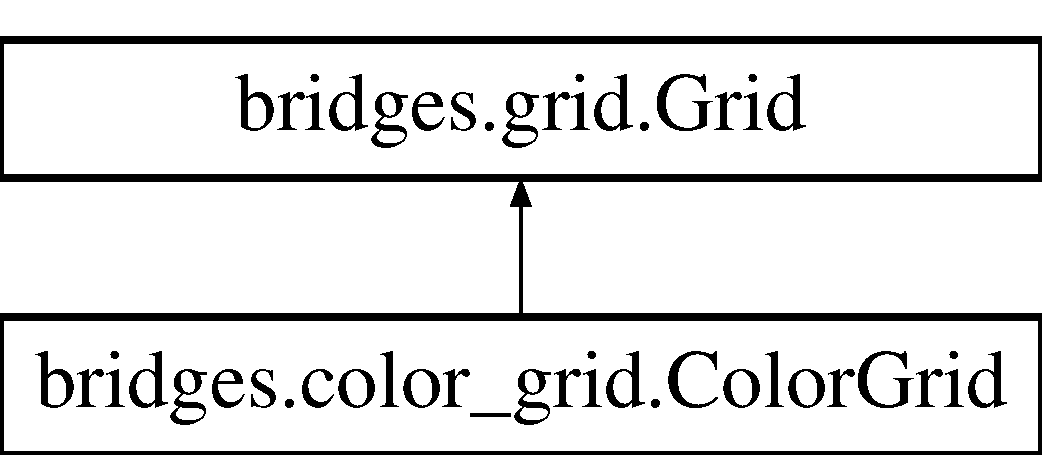
\includegraphics[height=2.000000cm]{classbridges_1_1grid_1_1_grid}
\end{center}
\end{figure}


\subsection{Detailed Description}
This is a base class in B\+R\+I\+D\+G\+ES for representing an (n x n) grid. 

\begin{DoxyAuthor}{Author}
David Burlinson, Matthew Mc\+Quaigue
\end{DoxyAuthor}
\begin{DoxyDate}{Date}
2018, 7/24/19, 2021
\end{DoxyDate}
\begin{DoxySeeAlso}{See also}
Color \hyperlink{namespacebridges_1_1grid}{grid} tutorial at \href{http://bridgesuncc.github.io/tutorials/Grid.html}{\tt http\+://bridgesuncc.\+github.\+io/tutorials/\+Grid.\+html} 
\end{DoxySeeAlso}
\subsection*{Public Member Functions}
\begin{DoxyCompactItemize}
\item 
def \hyperlink{classbridges_1_1grid_1_1_grid_ab1a040a486bbad5259fec54fb885eac1}{get\+\_\+data\+\_\+structure\+\_\+type} (self)
\begin{DoxyCompactList}\small\item\em Get the data structure type. \end{DoxyCompactList}\item 
def \hyperlink{classbridges_1_1grid_1_1_grid_a25587e3c0f450b336fc7bb11fc718c36}{\+\_\+\+\_\+init\+\_\+\+\_\+} (self, kwargs)
\begin{DoxyCompactList}\small\item\em \hyperlink{classbridges_1_1grid_1_1_grid}{Grid} constructor. \end{DoxyCompactList}\item 
def \hyperlink{classbridges_1_1grid_1_1_grid_a48f2107f2a2e970ada851012019a01dc}{dimensions} (self)
\begin{DoxyCompactList}\small\item\em Getter for the dimensions of the grid. \end{DoxyCompactList}\item 
def \hyperlink{classbridges_1_1grid_1_1_grid_a354c049fedceef226ff62aedf78c2a72}{get}
\begin{DoxyCompactList}\small\item\em Get the row,col element in the grid. \end{DoxyCompactList}\item 
def \hyperlink{classbridges_1_1grid_1_1_grid_a40d076434ad49fe29f6a931aba9f442b}{set}
\begin{DoxyCompactList}\small\item\em set the (row, col) element in the grid \end{DoxyCompactList}\end{DoxyCompactItemize}
\subsection*{Public Attributes}
\begin{DoxyCompactItemize}
\item 
\hyperlink{classbridges_1_1grid_1_1_grid_a609e662d769bbda34e88dd2be0307f4f}{grid}
\end{DoxyCompactItemize}
\subsection*{Static Public Attributes}
\begin{DoxyCompactItemize}
\item 
list \hyperlink{classbridges_1_1grid_1_1_grid_ac2ef408fca86892aceba252d1044fdee}{grid\+\_\+size} = \mbox{[}10, 10\mbox{]}
\item 
list \hyperlink{classbridges_1_1grid_1_1_grid_a5585d466b6738e4eee71a7dda56b4153}{max\+Grid\+Size} = \mbox{[}1080, 1920\mbox{]}
\end{DoxyCompactItemize}


\subsection{Constructor \& Destructor Documentation}
\mbox{\Hypertarget{classbridges_1_1grid_1_1_grid_a25587e3c0f450b336fc7bb11fc718c36}\label{classbridges_1_1grid_1_1_grid_a25587e3c0f450b336fc7bb11fc718c36}} 
\index{bridges\+::grid\+::\+Grid@{bridges\+::grid\+::\+Grid}!\+\_\+\+\_\+init\+\_\+\+\_\+@{\+\_\+\+\_\+init\+\_\+\+\_\+}}
\index{\+\_\+\+\_\+init\+\_\+\+\_\+@{\+\_\+\+\_\+init\+\_\+\+\_\+}!bridges\+::grid\+::\+Grid@{bridges\+::grid\+::\+Grid}}
\subsubsection{\texorpdfstring{\+\_\+\+\_\+init\+\_\+\+\_\+()}{\_\_init\_\_()}}
{\footnotesize\ttfamily def bridges.\+grid.\+Grid.\+\_\+\+\_\+init\+\_\+\+\_\+ (\begin{DoxyParamCaption}\item[{}]{self,  }\item[{}]{kwargs,  }\item[{}]{None }\end{DoxyParamCaption})}



\hyperlink{classbridges_1_1grid_1_1_grid}{Grid} constructor. 


\begin{DoxyParams}{Parameters}
{\em size} & size of the grid as array \\
\hline
{\em rows} & number of rows in grid \\
\hline
{\em cols} & number of the columns in grid \\
\hline
\end{DoxyParams}
\begin{DoxyReturn}{Returns}


None
\end{DoxyReturn}

\begin{DoxyExceptions}{Exceptions}
{\em Value\+Error} & if the size dimensions are greater than the max grid sizes (1080, 1920) \\
\hline
\end{DoxyExceptions}


\subsection{Member Function Documentation}
\mbox{\Hypertarget{classbridges_1_1grid_1_1_grid_a48f2107f2a2e970ada851012019a01dc}\label{classbridges_1_1grid_1_1_grid_a48f2107f2a2e970ada851012019a01dc}} 
\index{bridges\+::grid\+::\+Grid@{bridges\+::grid\+::\+Grid}!dimensions@{dimensions}}
\index{dimensions@{dimensions}!bridges\+::grid\+::\+Grid@{bridges\+::grid\+::\+Grid}}
\subsubsection{\texorpdfstring{dimensions()}{dimensions()}}
{\footnotesize\ttfamily def bridges.\+grid.\+Grid.\+dimensions (\begin{DoxyParamCaption}\item[{}]{self,  }\item[{}]{list }\end{DoxyParamCaption})}



Getter for the dimensions of the grid. 

\begin{DoxyReturn}{Returns}


list as the dimensions of the grid 
\end{DoxyReturn}
\mbox{\Hypertarget{classbridges_1_1grid_1_1_grid_a354c049fedceef226ff62aedf78c2a72}\label{classbridges_1_1grid_1_1_grid_a354c049fedceef226ff62aedf78c2a72}} 
\index{bridges\+::grid\+::\+Grid@{bridges\+::grid\+::\+Grid}!get@{get}}
\index{get@{get}!bridges\+::grid\+::\+Grid@{bridges\+::grid\+::\+Grid}}
\subsubsection{\texorpdfstring{get()}{get()}}
{\footnotesize\ttfamily def bridges.\+grid.\+Grid.\+get (\begin{DoxyParamCaption}\item[{}]{self,  }\item[{}]{row }\end{DoxyParamCaption})}



Get the row,col element in the grid. 

(int) row\+: row the element is in (int) col\+: col the element is in \begin{DoxyReturn}{Returns}


element 

none 

Raises 

Exception printing the traceback stack if returning the row and column is an error 
\end{DoxyReturn}
\mbox{\Hypertarget{classbridges_1_1grid_1_1_grid_ab1a040a486bbad5259fec54fb885eac1}\label{classbridges_1_1grid_1_1_grid_ab1a040a486bbad5259fec54fb885eac1}} 
\index{bridges\+::grid\+::\+Grid@{bridges\+::grid\+::\+Grid}!get\+\_\+data\+\_\+structure\+\_\+type@{get\+\_\+data\+\_\+structure\+\_\+type}}
\index{get\+\_\+data\+\_\+structure\+\_\+type@{get\+\_\+data\+\_\+structure\+\_\+type}!bridges\+::grid\+::\+Grid@{bridges\+::grid\+::\+Grid}}
\subsubsection{\texorpdfstring{get\+\_\+data\+\_\+structure\+\_\+type()}{get\_data\_structure\_type()}}
{\footnotesize\ttfamily def bridges.\+grid.\+Grid.\+get\+\_\+data\+\_\+structure\+\_\+type (\begin{DoxyParamCaption}\item[{}]{self,  }\item[{}]{str }\end{DoxyParamCaption})}



Get the data structure type. 

\begin{DoxyReturn}{Returns}


str representing the data structure type 
\end{DoxyReturn}
\mbox{\Hypertarget{classbridges_1_1grid_1_1_grid_a40d076434ad49fe29f6a931aba9f442b}\label{classbridges_1_1grid_1_1_grid_a40d076434ad49fe29f6a931aba9f442b}} 
\index{bridges\+::grid\+::\+Grid@{bridges\+::grid\+::\+Grid}!set@{set}}
\index{set@{set}!bridges\+::grid\+::\+Grid@{bridges\+::grid\+::\+Grid}}
\subsubsection{\texorpdfstring{set()}{set()}}
{\footnotesize\ttfamily def bridges.\+grid.\+Grid.\+set (\begin{DoxyParamCaption}\item[{}]{self,  }\item[{}]{row }\end{DoxyParamCaption})}



set the (row, col) element in the grid 


\begin{DoxyParams}{Parameters}
{\em row} & row position \\
\hline
{\em col} & column position \\
\hline
{\em val} & value to be set in (row, col) position \\
\hline
\end{DoxyParams}
\begin{DoxyReturn}{Returns}


None
\end{DoxyReturn}

\begin{DoxyExceptions}{Exceptions}
{\em Exception} & if setting the element at the row and column is a problem \\
\hline
\end{DoxyExceptions}


\subsection{Member Data Documentation}
\mbox{\Hypertarget{classbridges_1_1grid_1_1_grid_a609e662d769bbda34e88dd2be0307f4f}\label{classbridges_1_1grid_1_1_grid_a609e662d769bbda34e88dd2be0307f4f}} 
\index{bridges\+::grid\+::\+Grid@{bridges\+::grid\+::\+Grid}!grid@{grid}}
\index{grid@{grid}!bridges\+::grid\+::\+Grid@{bridges\+::grid\+::\+Grid}}
\subsubsection{\texorpdfstring{grid}{grid}}
{\footnotesize\ttfamily bridges.\+grid.\+Grid.\+grid}

\mbox{\Hypertarget{classbridges_1_1grid_1_1_grid_ac2ef408fca86892aceba252d1044fdee}\label{classbridges_1_1grid_1_1_grid_ac2ef408fca86892aceba252d1044fdee}} 
\index{bridges\+::grid\+::\+Grid@{bridges\+::grid\+::\+Grid}!grid\+\_\+size@{grid\+\_\+size}}
\index{grid\+\_\+size@{grid\+\_\+size}!bridges\+::grid\+::\+Grid@{bridges\+::grid\+::\+Grid}}
\subsubsection{\texorpdfstring{grid\+\_\+size}{grid\_size}}
{\footnotesize\ttfamily list bridges.\+grid.\+Grid.\+grid\+\_\+size = \mbox{[}10, 10\mbox{]}\hspace{0.3cm}{\ttfamily [static]}}

\mbox{\Hypertarget{classbridges_1_1grid_1_1_grid_a5585d466b6738e4eee71a7dda56b4153}\label{classbridges_1_1grid_1_1_grid_a5585d466b6738e4eee71a7dda56b4153}} 
\index{bridges\+::grid\+::\+Grid@{bridges\+::grid\+::\+Grid}!max\+Grid\+Size@{max\+Grid\+Size}}
\index{max\+Grid\+Size@{max\+Grid\+Size}!bridges\+::grid\+::\+Grid@{bridges\+::grid\+::\+Grid}}
\subsubsection{\texorpdfstring{max\+Grid\+Size}{maxGridSize}}
{\footnotesize\ttfamily list bridges.\+grid.\+Grid.\+max\+Grid\+Size = \mbox{[}1080, 1920\mbox{]}\hspace{0.3cm}{\ttfamily [static]}}



The documentation for this class was generated from the following file\+:\begin{DoxyCompactItemize}
\item 
/home/erik/work/bridges/bridges-\/python/bridges/\hyperlink{grid_8py}{grid.\+py}\end{DoxyCompactItemize}

\hypertarget{classbridges_1_1kd__tree__element_1_1_k_d_tree_element}{}\section{bridges.\+kd\+\_\+tree\+\_\+element.\+K\+D\+Tree\+Element Class Reference}
\label{classbridges_1_1kd__tree__element_1_1_k_d_tree_element}\index{bridges.kd\_tree\_element.KDTreeElement@{bridges.kd\_tree\_element.KDTreeElement}}
Inheritance diagram for bridges.\+kd\+\_\+tree\+\_\+element.\+K\+D\+Tree\+Element\+:\begin{figure}[H]
\begin{center}
\leavevmode
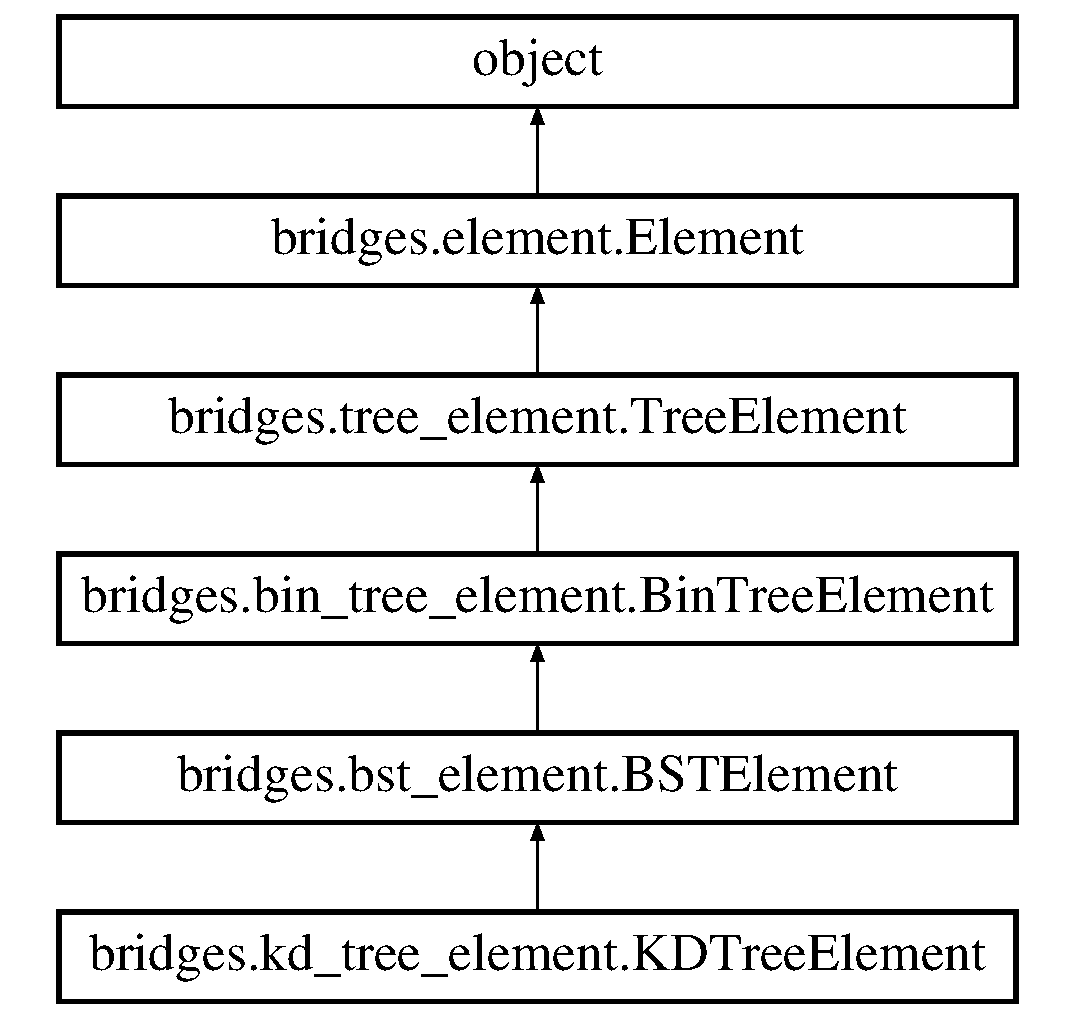
\includegraphics[height=5.000000cm]{classbridges_1_1kd__tree__element_1_1_k_d_tree_element}
\end{center}
\end{figure}


\subsection{Detailed Description}
The This class can be used to create K-\/d Tree elements, derived from B\+S\+T\+Element. 

K-\/D trees can be thought of as the spatial equivalent binary search trees and operate on multiple dimensions (2D and 3D are most common). These trees serve as a representation of the underlying geometrically defined spaces. Specialized versions of these trees include quadtrees and octrees, which subdivide into equal sized quadrants or octants at each level, respectively. This class extends the B\+S\+T\+Element class by adding a dimension property. It also includes a thickness property for displaying the partitioning lines generated by the convex decomposition.

\begin{DoxyAuthor}{Author}
Kalpathi Subramanian, Matthew Mc\+Quaigue 
\end{DoxyAuthor}
\begin{DoxyDate}{Date}
12/26/18, 7/23/19
\end{DoxyDate}
\begin{DoxySeeAlso}{See also}
Kd Tree tutorial, \href{http://bridgesuncc.github.io/tutorials/KdTree.html}{\texttt{ http\+://bridgesuncc.\+github.\+io/tutorials/\+Kd\+Tree.\+html}} 
\end{DoxySeeAlso}
\subsection*{Public Member Functions}
\begin{DoxyCompactItemize}
\item 
def \mbox{\hyperlink{classbridges_1_1kd__tree__element_1_1_k_d_tree_element_ad48f0bdabbb21cf83782efc1f8dbc1ed}{\+\_\+\+\_\+init\+\_\+\+\_\+}} (self, $\ast$$\ast$kwargs)
\begin{DoxyCompactList}\small\item\em Constructor bst element. \end{DoxyCompactList}\item 
str \mbox{\hyperlink{classbridges_1_1kd__tree__element_1_1_k_d_tree_element_a4b38af960542ccc8c3b74d90ee9570e2}{get\+\_\+data\+\_\+structure\+\_\+type}} (self)
\begin{DoxyCompactList}\small\item\em Getter for the data structure type. \end{DoxyCompactList}\item 
int \mbox{\hyperlink{classbridges_1_1kd__tree__element_1_1_k_d_tree_element_a2f600f754650ce8ea08954b969a5dae8}{dimension}} (self)
\begin{DoxyCompactList}\small\item\em Getter for the dimensions of the partition lines. \end{DoxyCompactList}\item 
None \mbox{\hyperlink{classbridges_1_1kd__tree__element_1_1_k_d_tree_element_a23ec48bd5d7949a2b1e62794344c87f9}{dimension}} (self, int dim)
\begin{DoxyCompactList}\small\item\em Setter for the dimension of th partitioning at this tree node. \end{DoxyCompactList}\item 
float \mbox{\hyperlink{classbridges_1_1kd__tree__element_1_1_k_d_tree_element_a936e2b664181ddc85e11a1c1057b3dab}{thickness}} (self)
\begin{DoxyCompactList}\small\item\em Getter for the thickness to the K\+D\+Tree partitions. \end{DoxyCompactList}\item 
None \mbox{\hyperlink{classbridges_1_1kd__tree__element_1_1_k_d_tree_element_ae78db83d6d61169f7afc9c8c4efcb87a}{thickness}} (self, th)
\begin{DoxyCompactList}\small\item\em Setter for the thickness of the K\+D\+Tree partitions -\/ can be used in the visualization. \end{DoxyCompactList}\item 
def \mbox{\hyperlink{classbridges_1_1kd__tree__element_1_1_k_d_tree_element_afa4f059c61b3cd9460199c9835641db2}{left}} (self)
\begin{DoxyCompactList}\small\item\em Getter for the left child of the tree element. \end{DoxyCompactList}\item 
def \mbox{\hyperlink{classbridges_1_1kd__tree__element_1_1_k_d_tree_element_a784bad6511dae3a7c769672d2d3af14f}{left}} (self, l)
\begin{DoxyCompactList}\small\item\em Setter for the left element in B\+ST. \end{DoxyCompactList}\item 
def \mbox{\hyperlink{classbridges_1_1kd__tree__element_1_1_k_d_tree_element_acbcfa46ba613daaf922d8b632b795a86}{right}} (self)
\begin{DoxyCompactList}\small\item\em Getter for the right child of the tree element. \end{DoxyCompactList}\item 
def \mbox{\hyperlink{classbridges_1_1kd__tree__element_1_1_k_d_tree_element_a89071f192bee403a44f92c86a5fdc49d}{right}} (self, r)
\begin{DoxyCompactList}\small\item\em Setter for the right element in B\+ST. \end{DoxyCompactList}\item 
def \mbox{\hyperlink{classbridges_1_1kd__tree__element_1_1_k_d_tree_element_a4e08a6f2e4ff70be2b0dfd6eacdcf10e}{get\+\_\+element\+\_\+representation}} (self)
\begin{DoxyCompactList}\small\item\em Augment the element with the \char`\"{}key\char`\"{} field. \end{DoxyCompactList}\end{DoxyCompactItemize}
\subsection*{Additional Inherited Members}


\subsection{Constructor \& Destructor Documentation}
\mbox{\Hypertarget{classbridges_1_1kd__tree__element_1_1_k_d_tree_element_ad48f0bdabbb21cf83782efc1f8dbc1ed}\label{classbridges_1_1kd__tree__element_1_1_k_d_tree_element_ad48f0bdabbb21cf83782efc1f8dbc1ed}} 
\index{bridges.kd\_tree\_element.KDTreeElement@{bridges.kd\_tree\_element.KDTreeElement}!\_\_init\_\_@{\_\_init\_\_}}
\index{\_\_init\_\_@{\_\_init\_\_}!bridges.kd\_tree\_element.KDTreeElement@{bridges.kd\_tree\_element.KDTreeElement}}
\subsubsection{\texorpdfstring{\_\_init\_\_()}{\_\_init\_\_()}}
{\footnotesize\ttfamily def bridges.\+kd\+\_\+tree\+\_\+element.\+K\+D\+Tree\+Element.\+\_\+\+\_\+init\+\_\+\+\_\+ (\begin{DoxyParamCaption}\item[{}]{self,  }\item[{$\ast$$\ast$}]{kwargs }\end{DoxyParamCaption})}



Constructor bst element. 

\begin{DoxyVerb}       (str) key: The label for the tree element that shows in visualization
       (generic) e: the generic object that the tree element will hold
       (BinTreeElement) left: the tree element assigned to child 0
       (BinTreeElement) right: the tree element assigned to child 1
\end{DoxyVerb}
 \begin{DoxyReturn}{Returns}


None 
\end{DoxyReturn}


Reimplemented from \mbox{\hyperlink{classbridges_1_1bst__element_1_1_b_s_t_element_a0be9b75a1da9322d40811669d13e05a4}{bridges.\+bst\+\_\+element.\+B\+S\+T\+Element}}.



\subsection{Member Function Documentation}
\mbox{\Hypertarget{classbridges_1_1kd__tree__element_1_1_k_d_tree_element_a2f600f754650ce8ea08954b969a5dae8}\label{classbridges_1_1kd__tree__element_1_1_k_d_tree_element_a2f600f754650ce8ea08954b969a5dae8}} 
\index{bridges.kd\_tree\_element.KDTreeElement@{bridges.kd\_tree\_element.KDTreeElement}!dimension@{dimension}}
\index{dimension@{dimension}!bridges.kd\_tree\_element.KDTreeElement@{bridges.kd\_tree\_element.KDTreeElement}}
\subsubsection{\texorpdfstring{dimension()}{dimension()}\hspace{0.1cm}{\footnotesize\ttfamily [1/2]}}
{\footnotesize\ttfamily  int bridges.\+kd\+\_\+tree\+\_\+element.\+K\+D\+Tree\+Element.\+dimension (\begin{DoxyParamCaption}\item[{}]{self }\end{DoxyParamCaption})}



Getter for the dimensions of the partition lines. 

\begin{DoxyReturn}{Returns}


int dimension (0, 1, 2, etc) 
\end{DoxyReturn}
\mbox{\Hypertarget{classbridges_1_1kd__tree__element_1_1_k_d_tree_element_a23ec48bd5d7949a2b1e62794344c87f9}\label{classbridges_1_1kd__tree__element_1_1_k_d_tree_element_a23ec48bd5d7949a2b1e62794344c87f9}} 
\index{bridges.kd\_tree\_element.KDTreeElement@{bridges.kd\_tree\_element.KDTreeElement}!dimension@{dimension}}
\index{dimension@{dimension}!bridges.kd\_tree\_element.KDTreeElement@{bridges.kd\_tree\_element.KDTreeElement}}
\subsubsection{\texorpdfstring{dimension()}{dimension()}\hspace{0.1cm}{\footnotesize\ttfamily [2/2]}}
{\footnotesize\ttfamily  None bridges.\+kd\+\_\+tree\+\_\+element.\+K\+D\+Tree\+Element.\+dimension (\begin{DoxyParamCaption}\item[{}]{self,  }\item[{int}]{dim }\end{DoxyParamCaption})}



Setter for the dimension of th partitioning at this tree node. 

\begin{DoxyVerb}       (int) dim: dimension value to set
\end{DoxyVerb}
 \begin{DoxyReturn}{Returns}


None 
\end{DoxyReturn}
\mbox{\Hypertarget{classbridges_1_1kd__tree__element_1_1_k_d_tree_element_a4b38af960542ccc8c3b74d90ee9570e2}\label{classbridges_1_1kd__tree__element_1_1_k_d_tree_element_a4b38af960542ccc8c3b74d90ee9570e2}} 
\index{bridges.kd\_tree\_element.KDTreeElement@{bridges.kd\_tree\_element.KDTreeElement}!get\_data\_structure\_type@{get\_data\_structure\_type}}
\index{get\_data\_structure\_type@{get\_data\_structure\_type}!bridges.kd\_tree\_element.KDTreeElement@{bridges.kd\_tree\_element.KDTreeElement}}
\subsubsection{\texorpdfstring{get\_data\_structure\_type()}{get\_data\_structure\_type()}}
{\footnotesize\ttfamily  str bridges.\+kd\+\_\+tree\+\_\+element.\+K\+D\+Tree\+Element.\+get\+\_\+data\+\_\+structure\+\_\+type (\begin{DoxyParamCaption}\item[{}]{self }\end{DoxyParamCaption})}



Getter for the data structure type. 

\begin{DoxyReturn}{Returns}


str of the the data structure type 
\end{DoxyReturn}


Reimplemented from \mbox{\hyperlink{classbridges_1_1bst__element_1_1_b_s_t_element_a8e655e06ba0f77b7e2681b6d291f39de}{bridges.\+bst\+\_\+element.\+B\+S\+T\+Element}}.

\mbox{\Hypertarget{classbridges_1_1kd__tree__element_1_1_k_d_tree_element_a4e08a6f2e4ff70be2b0dfd6eacdcf10e}\label{classbridges_1_1kd__tree__element_1_1_k_d_tree_element_a4e08a6f2e4ff70be2b0dfd6eacdcf10e}} 
\index{bridges.kd\_tree\_element.KDTreeElement@{bridges.kd\_tree\_element.KDTreeElement}!get\_element\_representation@{get\_element\_representation}}
\index{get\_element\_representation@{get\_element\_representation}!bridges.kd\_tree\_element.KDTreeElement@{bridges.kd\_tree\_element.KDTreeElement}}
\subsubsection{\texorpdfstring{get\_element\_representation()}{get\_element\_representation()}}
{\footnotesize\ttfamily def bridges.\+kd\+\_\+tree\+\_\+element.\+K\+D\+Tree\+Element.\+get\+\_\+element\+\_\+representation (\begin{DoxyParamCaption}\item[{}]{self }\end{DoxyParamCaption})}



Augment the element with the \char`\"{}key\char`\"{} field. 

\begin{DoxyReturn}{Returns}


dict representing the json of this tree 
\end{DoxyReturn}


Reimplemented from \mbox{\hyperlink{classbridges_1_1bst__element_1_1_b_s_t_element_a9d038f191a7cf06e75910463a3aa3b80}{bridges.\+bst\+\_\+element.\+B\+S\+T\+Element}}.

\mbox{\Hypertarget{classbridges_1_1kd__tree__element_1_1_k_d_tree_element_afa4f059c61b3cd9460199c9835641db2}\label{classbridges_1_1kd__tree__element_1_1_k_d_tree_element_afa4f059c61b3cd9460199c9835641db2}} 
\index{bridges.kd\_tree\_element.KDTreeElement@{bridges.kd\_tree\_element.KDTreeElement}!left@{left}}
\index{left@{left}!bridges.kd\_tree\_element.KDTreeElement@{bridges.kd\_tree\_element.KDTreeElement}}
\subsubsection{\texorpdfstring{left()}{left()}\hspace{0.1cm}{\footnotesize\ttfamily [1/2]}}
{\footnotesize\ttfamily def bridges.\+kd\+\_\+tree\+\_\+element.\+K\+D\+Tree\+Element.\+left (\begin{DoxyParamCaption}\item[{}]{self }\end{DoxyParamCaption})}



Getter for the left child of the tree element. 

\begin{DoxyReturn}{Returns}


Kd\+Tree\+Element the left child 
\end{DoxyReturn}


Reimplemented from \mbox{\hyperlink{classbridges_1_1bst__element_1_1_b_s_t_element_adb40ae0f98fe1cb7f153494c544d3f9f}{bridges.\+bst\+\_\+element.\+B\+S\+T\+Element}}.

\mbox{\Hypertarget{classbridges_1_1kd__tree__element_1_1_k_d_tree_element_a784bad6511dae3a7c769672d2d3af14f}\label{classbridges_1_1kd__tree__element_1_1_k_d_tree_element_a784bad6511dae3a7c769672d2d3af14f}} 
\index{bridges.kd\_tree\_element.KDTreeElement@{bridges.kd\_tree\_element.KDTreeElement}!left@{left}}
\index{left@{left}!bridges.kd\_tree\_element.KDTreeElement@{bridges.kd\_tree\_element.KDTreeElement}}
\subsubsection{\texorpdfstring{left()}{left()}\hspace{0.1cm}{\footnotesize\ttfamily [2/2]}}
{\footnotesize\ttfamily def bridges.\+kd\+\_\+tree\+\_\+element.\+K\+D\+Tree\+Element.\+left (\begin{DoxyParamCaption}\item[{}]{self,  }\item[{}]{l }\end{DoxyParamCaption})}



Setter for the left element in B\+ST. 


\begin{DoxyParams}{Parameters}
{\em l} & the value for the left child to be set as \\
\hline
\end{DoxyParams}


Reimplemented from \mbox{\hyperlink{classbridges_1_1bst__element_1_1_b_s_t_element_a0b45e63b73faabb6b969dd6222e07942}{bridges.\+bst\+\_\+element.\+B\+S\+T\+Element}}.

\mbox{\Hypertarget{classbridges_1_1kd__tree__element_1_1_k_d_tree_element_acbcfa46ba613daaf922d8b632b795a86}\label{classbridges_1_1kd__tree__element_1_1_k_d_tree_element_acbcfa46ba613daaf922d8b632b795a86}} 
\index{bridges.kd\_tree\_element.KDTreeElement@{bridges.kd\_tree\_element.KDTreeElement}!right@{right}}
\index{right@{right}!bridges.kd\_tree\_element.KDTreeElement@{bridges.kd\_tree\_element.KDTreeElement}}
\subsubsection{\texorpdfstring{right()}{right()}\hspace{0.1cm}{\footnotesize\ttfamily [1/2]}}
{\footnotesize\ttfamily def bridges.\+kd\+\_\+tree\+\_\+element.\+K\+D\+Tree\+Element.\+right (\begin{DoxyParamCaption}\item[{}]{self }\end{DoxyParamCaption})}



Getter for the right child of the tree element. 

\begin{DoxyReturn}{Returns}


Kd\+Tree\+Element the right child 
\end{DoxyReturn}


Reimplemented from \mbox{\hyperlink{classbridges_1_1bst__element_1_1_b_s_t_element_a3ec82fbc56a5e6309b69d2d963b483fd}{bridges.\+bst\+\_\+element.\+B\+S\+T\+Element}}.

\mbox{\Hypertarget{classbridges_1_1kd__tree__element_1_1_k_d_tree_element_a89071f192bee403a44f92c86a5fdc49d}\label{classbridges_1_1kd__tree__element_1_1_k_d_tree_element_a89071f192bee403a44f92c86a5fdc49d}} 
\index{bridges.kd\_tree\_element.KDTreeElement@{bridges.kd\_tree\_element.KDTreeElement}!right@{right}}
\index{right@{right}!bridges.kd\_tree\_element.KDTreeElement@{bridges.kd\_tree\_element.KDTreeElement}}
\subsubsection{\texorpdfstring{right()}{right()}\hspace{0.1cm}{\footnotesize\ttfamily [2/2]}}
{\footnotesize\ttfamily def bridges.\+kd\+\_\+tree\+\_\+element.\+K\+D\+Tree\+Element.\+right (\begin{DoxyParamCaption}\item[{}]{self,  }\item[{}]{r }\end{DoxyParamCaption})}



Setter for the right element in B\+ST. 


\begin{DoxyParams}{Parameters}
{\em r} & the value for the right child to be set as \\
\hline
\end{DoxyParams}


Reimplemented from \mbox{\hyperlink{classbridges_1_1bst__element_1_1_b_s_t_element_a978ae0db366dee59703ed266eebca0e9}{bridges.\+bst\+\_\+element.\+B\+S\+T\+Element}}.

\mbox{\Hypertarget{classbridges_1_1kd__tree__element_1_1_k_d_tree_element_a936e2b664181ddc85e11a1c1057b3dab}\label{classbridges_1_1kd__tree__element_1_1_k_d_tree_element_a936e2b664181ddc85e11a1c1057b3dab}} 
\index{bridges.kd\_tree\_element.KDTreeElement@{bridges.kd\_tree\_element.KDTreeElement}!thickness@{thickness}}
\index{thickness@{thickness}!bridges.kd\_tree\_element.KDTreeElement@{bridges.kd\_tree\_element.KDTreeElement}}
\subsubsection{\texorpdfstring{thickness()}{thickness()}\hspace{0.1cm}{\footnotesize\ttfamily [1/2]}}
{\footnotesize\ttfamily  float bridges.\+kd\+\_\+tree\+\_\+element.\+K\+D\+Tree\+Element.\+thickness (\begin{DoxyParamCaption}\item[{}]{self }\end{DoxyParamCaption})}



Getter for the thickness to the K\+D\+Tree partitions. 

\begin{DoxyReturn}{Returns}


float the thickness 
\end{DoxyReturn}
\mbox{\Hypertarget{classbridges_1_1kd__tree__element_1_1_k_d_tree_element_ae78db83d6d61169f7afc9c8c4efcb87a}\label{classbridges_1_1kd__tree__element_1_1_k_d_tree_element_ae78db83d6d61169f7afc9c8c4efcb87a}} 
\index{bridges.kd\_tree\_element.KDTreeElement@{bridges.kd\_tree\_element.KDTreeElement}!thickness@{thickness}}
\index{thickness@{thickness}!bridges.kd\_tree\_element.KDTreeElement@{bridges.kd\_tree\_element.KDTreeElement}}
\subsubsection{\texorpdfstring{thickness()}{thickness()}\hspace{0.1cm}{\footnotesize\ttfamily [2/2]}}
{\footnotesize\ttfamily  None bridges.\+kd\+\_\+tree\+\_\+element.\+K\+D\+Tree\+Element.\+thickness (\begin{DoxyParamCaption}\item[{}]{self,  }\item[{}]{th }\end{DoxyParamCaption})}



Setter for the thickness of the K\+D\+Tree partitions -\/ can be used in the visualization. 

\begin{DoxyVerb}       (float) th: thickness of partitions
\end{DoxyVerb}
 \begin{DoxyReturn}{Returns}


None 
\end{DoxyReturn}


The documentation for this class was generated from the following file\+:\begin{DoxyCompactItemize}
\item 
/\+Users/kalpathi/gr/bridges/python/bridges/\mbox{\hyperlink{kd__tree__element_8py}{kd\+\_\+tree\+\_\+element.\+py}}\end{DoxyCompactItemize}

\hypertarget{classbridges_1_1link__visualizer_1_1_link_visualizer}{}\section{bridges.\+link\+\_\+visualizer.\+Link\+Visualizer Class Reference}
\label{classbridges_1_1link__visualizer_1_1_link_visualizer}\index{bridges.\+link\+\_\+visualizer.\+Link\+Visualizer@{bridges.\+link\+\_\+visualizer.\+Link\+Visualizer}}


\subsection{Detailed Description}
This class maintains the visual attributes of links that join bridges elements. 

Visual properties include color, thickness, and opacity. Objects of this class are stored as part of the Element class. Generally, a user will manipulate the \hyperlink{classbridges_1_1link__visualizer_1_1_link_visualizer}{Link\+Visualizer} returned from the Element\textquotesingle{}s get\+Link\+Visualizer(\+Element it) method (which it is the bridges element this element is linked to), and then set attributes using its methods. Links are utilized in all types of linked lists, tree and graph structures.

Supported attribute values are as follows\+:

{\bfseries Supported Colors by name\+:} C\+SS colors; see the Color class for full list, or at https 

{\bfseries  Color by R\+G\+BA Specification \+:} Range\+: 0-\/255 for each component 

{\bfseries  Thickness\+: } Range \+: 0.\+0-\/50.\+0

{\bfseries  Opacity\+: } Range (0.\+0-\/1.\+0) 

\begin{DoxyAuthor}{Author}
Mihai Mehedint, Kalpathi Subramanian, Matthew Mc\+Quaigue
\end{DoxyAuthor}
\begin{DoxyDate}{Date}
2018, 6/24/19
\end{DoxyDate}
\begin{DoxySeeAlso}{See also}
Example Tutorial at ~\newline
 \href{http://bridgesuncc.github.io/Hello_World_Tutorials/SLL.html}{\tt http\+://bridgesuncc.\+github.\+io/\+Hello\+\_\+\+World\+\_\+\+Tutorials/\+S\+L\+L.\+html} 
\end{DoxySeeAlso}
\subsection*{Public Member Functions}
\begin{DoxyCompactItemize}
\item 
def \hyperlink{classbridges_1_1link__visualizer_1_1_link_visualizer_a9994004a7808bdcaa6f18ebfd9b7717a}{\+\_\+\+\_\+init\+\_\+\+\_\+} (self)
\begin{DoxyCompactList}\small\item\em Constructor for the link visualizer\textquotesingle{}. \end{DoxyCompactList}\item 
def \hyperlink{classbridges_1_1link__visualizer_1_1_link_visualizer_a4a89f95ecc6623ba17d2c47d7425c05b}{thickness} (self)
\begin{DoxyCompactList}\small\item\em Getter for the thickness of links visualization. \end{DoxyCompactList}\item 
def \hyperlink{classbridges_1_1link__visualizer_1_1_link_visualizer_af244bbe99885785f7dd3bb9460c1d21a}{thickness} (self, th)
\begin{DoxyCompactList}\small\item\em Setter for the thickness of links in visualization. \end{DoxyCompactList}\item 
def \hyperlink{classbridges_1_1link__visualizer_1_1_link_visualizer_ad87b36af48a35e41c9cad10239b4f7fb}{color} (self)
\begin{DoxyCompactList}\small\item\em Getter for the color of the link in the visualization. \end{DoxyCompactList}\item 
def \hyperlink{classbridges_1_1link__visualizer_1_1_link_visualizer_a3ae57af9d642648e0a581fd578084e08}{color} (self, args, kwargs)
\begin{DoxyCompactList}\small\item\em Setter for the color of the element in the bridges visualization. \end{DoxyCompactList}\item 
def \hyperlink{classbridges_1_1link__visualizer_1_1_link_visualizer_a777892e054f00e8ef0291c5d41ce7f75}{opacity} (self)
\begin{DoxyCompactList}\small\item\em Getter for the element opacity. \end{DoxyCompactList}\item 
def \hyperlink{classbridges_1_1link__visualizer_1_1_link_visualizer_acacbd654f9cdff27c8e10635b150f2c5}{opacity} (self, opacity)
\begin{DoxyCompactList}\small\item\em Setter for the elementopacity. \end{DoxyCompactList}\item 
def \hyperlink{classbridges_1_1link__visualizer_1_1_link_visualizer_afc00f309deac78e149f2e49f404de915}{label} (self)
\item 
def \hyperlink{classbridges_1_1link__visualizer_1_1_link_visualizer_a77a67a42f7f452715f7994cc9a791da9}{label} (self, l)
\item 
def \hyperlink{classbridges_1_1link__visualizer_1_1_link_visualizer_a4115c919bee0422f4f22308cba0c5c99}{get\+\_\+link\+\_\+properties} (self)
\begin{DoxyCompactList}\small\item\em Getter for the link properties. \end{DoxyCompactList}\item 
def \hyperlink{classbridges_1_1link__visualizer_1_1_link_visualizer_a36268a1bc712fb42f4401846e70536e6}{get\+\_\+label} (self)
\begin{DoxyCompactList}\small\item\em Getter for the link label. \end{DoxyCompactList}\item 
def \hyperlink{classbridges_1_1link__visualizer_1_1_link_visualizer_a51cb90a9162271fa083616321ae5faee}{set\+\_\+label} (self, \hyperlink{classbridges_1_1link__visualizer_1_1_link_visualizer_aace0e171fe2904f672b8ed3e0139343f}{label})
\begin{DoxyCompactList}\small\item\em Setter for the element label. \end{DoxyCompactList}\end{DoxyCompactItemize}
\subsection*{Public Attributes}
\begin{DoxyCompactItemize}
\item 
\hyperlink{classbridges_1_1link__visualizer_1_1_link_visualizer_aace0e171fe2904f672b8ed3e0139343f}{label}
\end{DoxyCompactItemize}


\subsection{Constructor \& Destructor Documentation}
\mbox{\Hypertarget{classbridges_1_1link__visualizer_1_1_link_visualizer_a9994004a7808bdcaa6f18ebfd9b7717a}\label{classbridges_1_1link__visualizer_1_1_link_visualizer_a9994004a7808bdcaa6f18ebfd9b7717a}} 
\index{bridges\+::link\+\_\+visualizer\+::\+Link\+Visualizer@{bridges\+::link\+\_\+visualizer\+::\+Link\+Visualizer}!\+\_\+\+\_\+init\+\_\+\+\_\+@{\+\_\+\+\_\+init\+\_\+\+\_\+}}
\index{\+\_\+\+\_\+init\+\_\+\+\_\+@{\+\_\+\+\_\+init\+\_\+\+\_\+}!bridges\+::link\+\_\+visualizer\+::\+Link\+Visualizer@{bridges\+::link\+\_\+visualizer\+::\+Link\+Visualizer}}
\subsubsection{\texorpdfstring{\+\_\+\+\_\+init\+\_\+\+\_\+()}{\_\_init\_\_()}}
{\footnotesize\ttfamily def bridges.\+link\+\_\+visualizer.\+Link\+Visualizer.\+\_\+\+\_\+init\+\_\+\+\_\+ (\begin{DoxyParamCaption}\item[{}]{self,  }\item[{}]{None }\end{DoxyParamCaption})}



Constructor for the link visualizer\textquotesingle{}. 

\begin{DoxyParagraph}{Retruns}
None 
\end{DoxyParagraph}


\subsection{Member Function Documentation}
\mbox{\Hypertarget{classbridges_1_1link__visualizer_1_1_link_visualizer_ad87b36af48a35e41c9cad10239b4f7fb}\label{classbridges_1_1link__visualizer_1_1_link_visualizer_ad87b36af48a35e41c9cad10239b4f7fb}} 
\index{bridges\+::link\+\_\+visualizer\+::\+Link\+Visualizer@{bridges\+::link\+\_\+visualizer\+::\+Link\+Visualizer}!color@{color}}
\index{color@{color}!bridges\+::link\+\_\+visualizer\+::\+Link\+Visualizer@{bridges\+::link\+\_\+visualizer\+::\+Link\+Visualizer}}
\subsubsection{\texorpdfstring{color()}{color()}\hspace{0.1cm}{\footnotesize\ttfamily [1/2]}}
{\footnotesize\ttfamily def bridges.\+link\+\_\+visualizer.\+Link\+Visualizer.\+color (\begin{DoxyParamCaption}\item[{}]{self,  }\item[{}]{Color }\end{DoxyParamCaption})}



Getter for the color of the link in the visualization. 

\begin{DoxyReturn}{Returns}


Color 
\end{DoxyReturn}
\mbox{\Hypertarget{classbridges_1_1link__visualizer_1_1_link_visualizer_a3ae57af9d642648e0a581fd578084e08}\label{classbridges_1_1link__visualizer_1_1_link_visualizer_a3ae57af9d642648e0a581fd578084e08}} 
\index{bridges\+::link\+\_\+visualizer\+::\+Link\+Visualizer@{bridges\+::link\+\_\+visualizer\+::\+Link\+Visualizer}!color@{color}}
\index{color@{color}!bridges\+::link\+\_\+visualizer\+::\+Link\+Visualizer@{bridges\+::link\+\_\+visualizer\+::\+Link\+Visualizer}}
\subsubsection{\texorpdfstring{color()}{color()}\hspace{0.1cm}{\footnotesize\ttfamily [2/2]}}
{\footnotesize\ttfamily def bridges.\+link\+\_\+visualizer.\+Link\+Visualizer.\+color (\begin{DoxyParamCaption}\item[{}]{self,  }\item[{}]{args,  }\item[{}]{kwargs }\end{DoxyParamCaption})}



Setter for the color of the element in the bridges visualization. 

(optional) list\+: requires either 3 ints 0-\/255 for R\+GB and an optional float 0.\+0-\/1.\+0 for alpha EX\+: color = \mbox{[}0, 255, 0, 1.\+0\mbox{]}. (optional) str\+: string representing the element color. Supported web colors\+: \href{https://developer.mozilla.org/en-US/docs/Web/CSS/color_value}{\tt https\+://developer.\+mozilla.\+org/en-\/\+U\+S/docs/\+Web/\+C\+S\+S/color\+\_\+value} \begin{DoxyReturn}{Returns}


None
\end{DoxyReturn}

\begin{DoxyExceptions}{Exceptions}
{\em Value\+Error} & if the color name provided is not available \\
\hline
\end{DoxyExceptions}
\mbox{\Hypertarget{classbridges_1_1link__visualizer_1_1_link_visualizer_a36268a1bc712fb42f4401846e70536e6}\label{classbridges_1_1link__visualizer_1_1_link_visualizer_a36268a1bc712fb42f4401846e70536e6}} 
\index{bridges\+::link\+\_\+visualizer\+::\+Link\+Visualizer@{bridges\+::link\+\_\+visualizer\+::\+Link\+Visualizer}!get\+\_\+label@{get\+\_\+label}}
\index{get\+\_\+label@{get\+\_\+label}!bridges\+::link\+\_\+visualizer\+::\+Link\+Visualizer@{bridges\+::link\+\_\+visualizer\+::\+Link\+Visualizer}}
\subsubsection{\texorpdfstring{get\+\_\+label()}{get\_label()}}
{\footnotesize\ttfamily def bridges.\+link\+\_\+visualizer.\+Link\+Visualizer.\+get\+\_\+label (\begin{DoxyParamCaption}\item[{}]{self }\end{DoxyParamCaption})}



Getter for the link label. 

\begin{DoxyReturn}{Returns}


string link label 
\end{DoxyReturn}
\mbox{\Hypertarget{classbridges_1_1link__visualizer_1_1_link_visualizer_a4115c919bee0422f4f22308cba0c5c99}\label{classbridges_1_1link__visualizer_1_1_link_visualizer_a4115c919bee0422f4f22308cba0c5c99}} 
\index{bridges\+::link\+\_\+visualizer\+::\+Link\+Visualizer@{bridges\+::link\+\_\+visualizer\+::\+Link\+Visualizer}!get\+\_\+link\+\_\+properties@{get\+\_\+link\+\_\+properties}}
\index{get\+\_\+link\+\_\+properties@{get\+\_\+link\+\_\+properties}!bridges\+::link\+\_\+visualizer\+::\+Link\+Visualizer@{bridges\+::link\+\_\+visualizer\+::\+Link\+Visualizer}}
\subsubsection{\texorpdfstring{get\+\_\+link\+\_\+properties()}{get\_link\_properties()}}
{\footnotesize\ttfamily def bridges.\+link\+\_\+visualizer.\+Link\+Visualizer.\+get\+\_\+link\+\_\+properties (\begin{DoxyParamCaption}\item[{}]{self }\end{DoxyParamCaption})}



Getter for the link properties. 

\begin{DoxyReturn}{Returns}


dict link properties 
\end{DoxyReturn}
\mbox{\Hypertarget{classbridges_1_1link__visualizer_1_1_link_visualizer_afc00f309deac78e149f2e49f404de915}\label{classbridges_1_1link__visualizer_1_1_link_visualizer_afc00f309deac78e149f2e49f404de915}} 
\index{bridges\+::link\+\_\+visualizer\+::\+Link\+Visualizer@{bridges\+::link\+\_\+visualizer\+::\+Link\+Visualizer}!label@{label}}
\index{label@{label}!bridges\+::link\+\_\+visualizer\+::\+Link\+Visualizer@{bridges\+::link\+\_\+visualizer\+::\+Link\+Visualizer}}
\subsubsection{\texorpdfstring{label()}{label()}\hspace{0.1cm}{\footnotesize\ttfamily [1/2]}}
{\footnotesize\ttfamily def bridges.\+link\+\_\+visualizer.\+Link\+Visualizer.\+label (\begin{DoxyParamCaption}\item[{}]{self }\end{DoxyParamCaption})}

\mbox{\Hypertarget{classbridges_1_1link__visualizer_1_1_link_visualizer_a77a67a42f7f452715f7994cc9a791da9}\label{classbridges_1_1link__visualizer_1_1_link_visualizer_a77a67a42f7f452715f7994cc9a791da9}} 
\index{bridges\+::link\+\_\+visualizer\+::\+Link\+Visualizer@{bridges\+::link\+\_\+visualizer\+::\+Link\+Visualizer}!label@{label}}
\index{label@{label}!bridges\+::link\+\_\+visualizer\+::\+Link\+Visualizer@{bridges\+::link\+\_\+visualizer\+::\+Link\+Visualizer}}
\subsubsection{\texorpdfstring{label()}{label()}\hspace{0.1cm}{\footnotesize\ttfamily [2/2]}}
{\footnotesize\ttfamily def bridges.\+link\+\_\+visualizer.\+Link\+Visualizer.\+label (\begin{DoxyParamCaption}\item[{}]{self,  }\item[{}]{l }\end{DoxyParamCaption})}

\mbox{\Hypertarget{classbridges_1_1link__visualizer_1_1_link_visualizer_a777892e054f00e8ef0291c5d41ce7f75}\label{classbridges_1_1link__visualizer_1_1_link_visualizer_a777892e054f00e8ef0291c5d41ce7f75}} 
\index{bridges\+::link\+\_\+visualizer\+::\+Link\+Visualizer@{bridges\+::link\+\_\+visualizer\+::\+Link\+Visualizer}!opacity@{opacity}}
\index{opacity@{opacity}!bridges\+::link\+\_\+visualizer\+::\+Link\+Visualizer@{bridges\+::link\+\_\+visualizer\+::\+Link\+Visualizer}}
\subsubsection{\texorpdfstring{opacity()}{opacity()}\hspace{0.1cm}{\footnotesize\ttfamily [1/2]}}
{\footnotesize\ttfamily def bridges.\+link\+\_\+visualizer.\+Link\+Visualizer.\+opacity (\begin{DoxyParamCaption}\item[{}]{self }\end{DoxyParamCaption})}



Getter for the element opacity. 

\begin{DoxyReturn}{Returns}


opacity element opacity 
\end{DoxyReturn}
\mbox{\Hypertarget{classbridges_1_1link__visualizer_1_1_link_visualizer_acacbd654f9cdff27c8e10635b150f2c5}\label{classbridges_1_1link__visualizer_1_1_link_visualizer_acacbd654f9cdff27c8e10635b150f2c5}} 
\index{bridges\+::link\+\_\+visualizer\+::\+Link\+Visualizer@{bridges\+::link\+\_\+visualizer\+::\+Link\+Visualizer}!opacity@{opacity}}
\index{opacity@{opacity}!bridges\+::link\+\_\+visualizer\+::\+Link\+Visualizer@{bridges\+::link\+\_\+visualizer\+::\+Link\+Visualizer}}
\subsubsection{\texorpdfstring{opacity()}{opacity()}\hspace{0.1cm}{\footnotesize\ttfamily [2/2]}}
{\footnotesize\ttfamily def bridges.\+link\+\_\+visualizer.\+Link\+Visualizer.\+opacity (\begin{DoxyParamCaption}\item[{}]{self,  }\item[{}]{opacity }\end{DoxyParamCaption})}



Setter for the elementopacity. 


\begin{DoxyParams}{Parameters}
{\em opacity} & opacity value (0-\/1.\+0) to set \\
\hline
\end{DoxyParams}
\begin{DoxyReturn}{Returns}


None 
\end{DoxyReturn}
\mbox{\Hypertarget{classbridges_1_1link__visualizer_1_1_link_visualizer_a51cb90a9162271fa083616321ae5faee}\label{classbridges_1_1link__visualizer_1_1_link_visualizer_a51cb90a9162271fa083616321ae5faee}} 
\index{bridges\+::link\+\_\+visualizer\+::\+Link\+Visualizer@{bridges\+::link\+\_\+visualizer\+::\+Link\+Visualizer}!set\+\_\+label@{set\+\_\+label}}
\index{set\+\_\+label@{set\+\_\+label}!bridges\+::link\+\_\+visualizer\+::\+Link\+Visualizer@{bridges\+::link\+\_\+visualizer\+::\+Link\+Visualizer}}
\subsubsection{\texorpdfstring{set\+\_\+label()}{set\_label()}}
{\footnotesize\ttfamily def bridges.\+link\+\_\+visualizer.\+Link\+Visualizer.\+set\+\_\+label (\begin{DoxyParamCaption}\item[{}]{self,  }\item[{}]{label }\end{DoxyParamCaption})}



Setter for the element label. 


\begin{DoxyParams}{Parameters}
{\em label} & link label (string) \\
\hline
\end{DoxyParams}
\begin{DoxyReturn}{Returns}


None 
\end{DoxyReturn}
\mbox{\Hypertarget{classbridges_1_1link__visualizer_1_1_link_visualizer_a4a89f95ecc6623ba17d2c47d7425c05b}\label{classbridges_1_1link__visualizer_1_1_link_visualizer_a4a89f95ecc6623ba17d2c47d7425c05b}} 
\index{bridges\+::link\+\_\+visualizer\+::\+Link\+Visualizer@{bridges\+::link\+\_\+visualizer\+::\+Link\+Visualizer}!thickness@{thickness}}
\index{thickness@{thickness}!bridges\+::link\+\_\+visualizer\+::\+Link\+Visualizer@{bridges\+::link\+\_\+visualizer\+::\+Link\+Visualizer}}
\subsubsection{\texorpdfstring{thickness()}{thickness()}\hspace{0.1cm}{\footnotesize\ttfamily [1/2]}}
{\footnotesize\ttfamily def bridges.\+link\+\_\+visualizer.\+Link\+Visualizer.\+thickness (\begin{DoxyParamCaption}\item[{}]{self,  }\item[{}]{float }\end{DoxyParamCaption})}



Getter for the thickness of links visualization. 

\begin{DoxyReturn}{Returns}


float the thickness 
\end{DoxyReturn}
\mbox{\Hypertarget{classbridges_1_1link__visualizer_1_1_link_visualizer_af244bbe99885785f7dd3bb9460c1d21a}\label{classbridges_1_1link__visualizer_1_1_link_visualizer_af244bbe99885785f7dd3bb9460c1d21a}} 
\index{bridges\+::link\+\_\+visualizer\+::\+Link\+Visualizer@{bridges\+::link\+\_\+visualizer\+::\+Link\+Visualizer}!thickness@{thickness}}
\index{thickness@{thickness}!bridges\+::link\+\_\+visualizer\+::\+Link\+Visualizer@{bridges\+::link\+\_\+visualizer\+::\+Link\+Visualizer}}
\subsubsection{\texorpdfstring{thickness()}{thickness()}\hspace{0.1cm}{\footnotesize\ttfamily [2/2]}}
{\footnotesize\ttfamily def bridges.\+link\+\_\+visualizer.\+Link\+Visualizer.\+thickness (\begin{DoxyParamCaption}\item[{}]{self,  }\item[{}]{th }\end{DoxyParamCaption})}



Setter for the thickness of links in visualization. 

(float) th\+: the thickness to be applied to the link \begin{DoxyReturn}{Returns}


None 
\end{DoxyReturn}


\subsection{Member Data Documentation}
\mbox{\Hypertarget{classbridges_1_1link__visualizer_1_1_link_visualizer_aace0e171fe2904f672b8ed3e0139343f}\label{classbridges_1_1link__visualizer_1_1_link_visualizer_aace0e171fe2904f672b8ed3e0139343f}} 
\index{bridges\+::link\+\_\+visualizer\+::\+Link\+Visualizer@{bridges\+::link\+\_\+visualizer\+::\+Link\+Visualizer}!label@{label}}
\index{label@{label}!bridges\+::link\+\_\+visualizer\+::\+Link\+Visualizer@{bridges\+::link\+\_\+visualizer\+::\+Link\+Visualizer}}
\subsubsection{\texorpdfstring{label}{label}}
{\footnotesize\ttfamily bridges.\+link\+\_\+visualizer.\+Link\+Visualizer.\+label}



The documentation for this class was generated from the following file\+:\begin{DoxyCompactItemize}
\item 
/home/erik/work/bridges/bridges-\/python/bridges/\hyperlink{link__visualizer_8py}{link\+\_\+visualizer.\+py}\end{DoxyCompactItemize}

\hypertarget{classbridges_1_1ml__element_1_1_m_lelement}{}\section{bridges.\+ml\+\_\+element.\+M\+Lelement Class Reference}
\label{classbridges_1_1ml__element_1_1_m_lelement}\index{bridges.\+ml\+\_\+element.\+M\+Lelement@{bridges.\+ml\+\_\+element.\+M\+Lelement}}
Inheritance diagram for bridges.\+ml\+\_\+element.\+M\+Lelement\+:\begin{figure}[H]
\begin{center}
\leavevmode
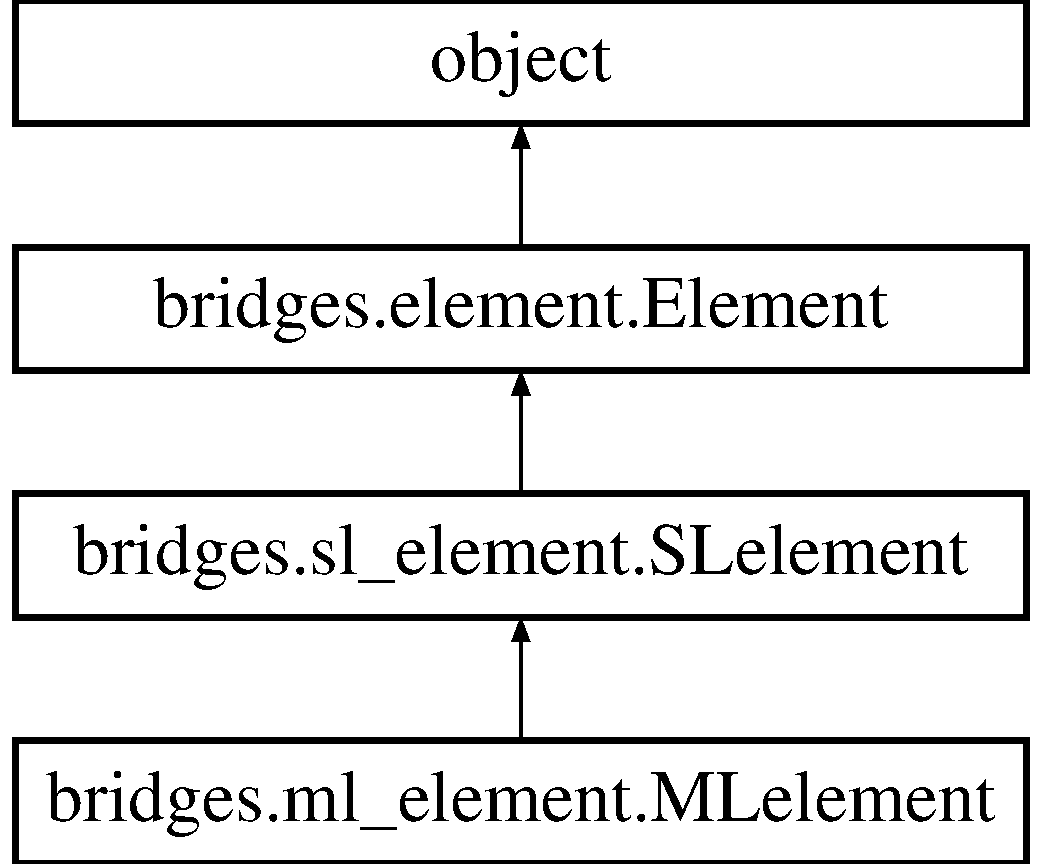
\includegraphics[height=3.000000cm]{classbridges_1_1ml__element_1_1_m_lelement}
\end{center}
\end{figure}


\subsection{Detailed Description}
This class can be used to instantiate Multi-\/list Elements. 

This class extends S\+Lelement (singly linked list element) to build multi-\/lists; Multilist elements contain a tag (boolean) that indicates if the element contains a sublist or not; if the tag is true, then there is a sublist beginning at this node and the starting point is the `sublist\textquotesingle{} field in the element. If the tag is false, then the list continues as a normal singly linked list. The sublists are re recursive\+: any sublist can have its own sublists and so on. As in singly linked elements, the next pointer points to the following list element and each element contains a generic application specific object.

Multi-\/list elements contain a visualizer (Element\+Visualizer) object for setting visual attributes (color, shape, opacity, size), necessary for displaying them in a web browser.

Elements also have a Link\+Visualizer object, that is used when they are linked to another element, appropriate for setting link attributes, for instance, between the current element and its next element. In this case, the link in question is that which connects the element to the following elements; a similar logic follows for sublists.

\begin{DoxyAuthor}{Author}
Kalpathi Subramanian, Matthew Mc\+Quaigue
\end{DoxyAuthor}
\begin{DoxyDate}{Date}
2018, 7/23/19, 2021
\end{DoxyDate}
\begin{DoxySeeAlso}{See also}
There is a tutorial about Multi Lists \+: \href{http://bridgesuncc.github.io/tutorials/ML.html}{\tt http\+://bridgesuncc.\+github.\+io/tutorials/\+M\+L.\+html} 
\end{DoxySeeAlso}
\subsection*{Public Member Functions}
\begin{DoxyCompactItemize}
\item 
def \hyperlink{classbridges_1_1ml__element_1_1_m_lelement_ae0242b9e3f2d7d7ccc702ef0bc7a61ba}{\+\_\+\+\_\+init\+\_\+\+\_\+} (self, kwargs)
\begin{DoxyCompactList}\small\item\em Constructor for \hyperlink{classbridges_1_1ml__element_1_1_m_lelement}{M\+Lelement}. \end{DoxyCompactList}\item 
def \hyperlink{classbridges_1_1ml__element_1_1_m_lelement_a1b02783280dacd20982bb06a1e3070f4}{sub\+\_\+list} (self)
\begin{DoxyCompactList}\small\item\em Getter for the sublist at this node if exists. \end{DoxyCompactList}\item 
def \hyperlink{classbridges_1_1ml__element_1_1_m_lelement_a8ad12079b474fb676f49aed7bacd5e10}{sub\+\_\+list} (self, sl)
\begin{DoxyCompactList}\small\item\em Setter for the start of a new sublist. \end{DoxyCompactList}\item 
def \hyperlink{classbridges_1_1ml__element_1_1_m_lelement_a97693d616263a8ee59b066829e8ce7e8}{get\+\_\+data\+\_\+structure\+\_\+type} (self)
\begin{DoxyCompactList}\small\item\em Getter for the data structure type. \end{DoxyCompactList}\item 
def \hyperlink{classbridges_1_1ml__element_1_1_m_lelement_a951d30261514e6eaefdd7d60f1c77f73}{next} (self)
\begin{DoxyCompactList}\small\item\em Retrieves the element following this element. \end{DoxyCompactList}\item 
def \hyperlink{classbridges_1_1ml__element_1_1_m_lelement_a588b700bb42eb43ce3993f9715497deb}{next} (self, n)
\item 
def \hyperlink{classbridges_1_1ml__element_1_1_m_lelement_a805f6b6f24ec9c5518c298320742a8d6}{tag} (self)
\begin{DoxyCompactList}\small\item\em Getter for the tag of the element. \end{DoxyCompactList}\item 
def \hyperlink{classbridges_1_1ml__element_1_1_m_lelement_aaae13135b666038dee8a843cd32b03b1}{tag} (self, t)
\begin{DoxyCompactList}\small\item\em Setter for the tag of the element. \end{DoxyCompactList}\item 
def \hyperlink{classbridges_1_1ml__element_1_1_m_lelement_a7d176b966746a889f9234d4a76b99c0c}{get\+\_\+data\+\_\+structure\+\_\+representation} (self)
\begin{DoxyCompactList}\small\item\em Getter for the data structure representation. \end{DoxyCompactList}\item 
def \hyperlink{classbridges_1_1ml__element_1_1_m_lelement_a3996cd2cec7c3978437392eba2ef66eb}{get\+\_\+list\+\_\+elements} (self, nodes)
\begin{DoxyCompactList}\small\item\em Getter for the elements of the list. \end{DoxyCompactList}\end{DoxyCompactItemize}
\subsection*{Additional Inherited Members}


\subsection{Constructor \& Destructor Documentation}
\mbox{\Hypertarget{classbridges_1_1ml__element_1_1_m_lelement_ae0242b9e3f2d7d7ccc702ef0bc7a61ba}\label{classbridges_1_1ml__element_1_1_m_lelement_ae0242b9e3f2d7d7ccc702ef0bc7a61ba}} 
\index{bridges\+::ml\+\_\+element\+::\+M\+Lelement@{bridges\+::ml\+\_\+element\+::\+M\+Lelement}!\+\_\+\+\_\+init\+\_\+\+\_\+@{\+\_\+\+\_\+init\+\_\+\+\_\+}}
\index{\+\_\+\+\_\+init\+\_\+\+\_\+@{\+\_\+\+\_\+init\+\_\+\+\_\+}!bridges\+::ml\+\_\+element\+::\+M\+Lelement@{bridges\+::ml\+\_\+element\+::\+M\+Lelement}}
\subsubsection{\texorpdfstring{\+\_\+\+\_\+init\+\_\+\+\_\+()}{\_\_init\_\_()}}
{\footnotesize\ttfamily def bridges.\+ml\+\_\+element.\+M\+Lelement.\+\_\+\+\_\+init\+\_\+\+\_\+ (\begin{DoxyParamCaption}\item[{}]{self,  }\item[{}]{kwargs,  }\item[{}]{None }\end{DoxyParamCaption})}



Constructor for \hyperlink{classbridges_1_1ml__element_1_1_m_lelement}{M\+Lelement}. 

(str) label\+: the label the S\+Lelement will hold and show on bridges visualization (object) e\+: the generic object/value that this S\+Lelement will hold (object) next\+: the next element that will be assigned to this S\+Lelement next pointer 
\begin{DoxyParams}{Parameters}
{\em sublist} & the \hyperlink{classbridges_1_1ml__element_1_1_m_lelement}{M\+Lelement} that is the beginning of a sublist \\
\hline
\end{DoxyParams}
\begin{DoxyReturn}{Returns}


None 
\end{DoxyReturn}


\subsection{Member Function Documentation}
\mbox{\Hypertarget{classbridges_1_1ml__element_1_1_m_lelement_a7d176b966746a889f9234d4a76b99c0c}\label{classbridges_1_1ml__element_1_1_m_lelement_a7d176b966746a889f9234d4a76b99c0c}} 
\index{bridges\+::ml\+\_\+element\+::\+M\+Lelement@{bridges\+::ml\+\_\+element\+::\+M\+Lelement}!get\+\_\+data\+\_\+structure\+\_\+representation@{get\+\_\+data\+\_\+structure\+\_\+representation}}
\index{get\+\_\+data\+\_\+structure\+\_\+representation@{get\+\_\+data\+\_\+structure\+\_\+representation}!bridges\+::ml\+\_\+element\+::\+M\+Lelement@{bridges\+::ml\+\_\+element\+::\+M\+Lelement}}
\subsubsection{\texorpdfstring{get\+\_\+data\+\_\+structure\+\_\+representation()}{get\_data\_structure\_representation()}}
{\footnotesize\ttfamily def bridges.\+ml\+\_\+element.\+M\+Lelement.\+get\+\_\+data\+\_\+structure\+\_\+representation (\begin{DoxyParamCaption}\item[{}]{self,  }\item[{}]{dict }\end{DoxyParamCaption})}



Getter for the data structure representation. 

\begin{DoxyReturn}{Returns}


dict representing the json structure before dumping 
\end{DoxyReturn}
\mbox{\Hypertarget{classbridges_1_1ml__element_1_1_m_lelement_a97693d616263a8ee59b066829e8ce7e8}\label{classbridges_1_1ml__element_1_1_m_lelement_a97693d616263a8ee59b066829e8ce7e8}} 
\index{bridges\+::ml\+\_\+element\+::\+M\+Lelement@{bridges\+::ml\+\_\+element\+::\+M\+Lelement}!get\+\_\+data\+\_\+structure\+\_\+type@{get\+\_\+data\+\_\+structure\+\_\+type}}
\index{get\+\_\+data\+\_\+structure\+\_\+type@{get\+\_\+data\+\_\+structure\+\_\+type}!bridges\+::ml\+\_\+element\+::\+M\+Lelement@{bridges\+::ml\+\_\+element\+::\+M\+Lelement}}
\subsubsection{\texorpdfstring{get\+\_\+data\+\_\+structure\+\_\+type()}{get\_data\_structure\_type()}}
{\footnotesize\ttfamily def bridges.\+ml\+\_\+element.\+M\+Lelement.\+get\+\_\+data\+\_\+structure\+\_\+type (\begin{DoxyParamCaption}\item[{}]{self,  }\item[{}]{str }\end{DoxyParamCaption})}



Getter for the data structure type. 

\begin{DoxyReturn}{Returns}


str representing the type 
\end{DoxyReturn}
\mbox{\Hypertarget{classbridges_1_1ml__element_1_1_m_lelement_a3996cd2cec7c3978437392eba2ef66eb}\label{classbridges_1_1ml__element_1_1_m_lelement_a3996cd2cec7c3978437392eba2ef66eb}} 
\index{bridges\+::ml\+\_\+element\+::\+M\+Lelement@{bridges\+::ml\+\_\+element\+::\+M\+Lelement}!get\+\_\+list\+\_\+elements@{get\+\_\+list\+\_\+elements}}
\index{get\+\_\+list\+\_\+elements@{get\+\_\+list\+\_\+elements}!bridges\+::ml\+\_\+element\+::\+M\+Lelement@{bridges\+::ml\+\_\+element\+::\+M\+Lelement}}
\subsubsection{\texorpdfstring{get\+\_\+list\+\_\+elements()}{get\_list\_elements()}}
{\footnotesize\ttfamily def bridges.\+ml\+\_\+element.\+M\+Lelement.\+get\+\_\+list\+\_\+elements (\begin{DoxyParamCaption}\item[{}]{self,  }\item[{}]{nodes }\end{DoxyParamCaption})}



Getter for the elements of the list. 


\begin{DoxyParams}{Parameters}
{\em nodes} & a list of the nodes \\
\hline
\end{DoxyParams}
\begin{DoxyReturn}{Returns}


element 
\end{DoxyReturn}
\mbox{\Hypertarget{classbridges_1_1ml__element_1_1_m_lelement_a951d30261514e6eaefdd7d60f1c77f73}\label{classbridges_1_1ml__element_1_1_m_lelement_a951d30261514e6eaefdd7d60f1c77f73}} 
\index{bridges\+::ml\+\_\+element\+::\+M\+Lelement@{bridges\+::ml\+\_\+element\+::\+M\+Lelement}!next@{next}}
\index{next@{next}!bridges\+::ml\+\_\+element\+::\+M\+Lelement@{bridges\+::ml\+\_\+element\+::\+M\+Lelement}}
\subsubsection{\texorpdfstring{next()}{next()}\hspace{0.1cm}{\footnotesize\ttfamily [1/2]}}
{\footnotesize\ttfamily def bridges.\+ml\+\_\+element.\+M\+Lelement.\+next (\begin{DoxyParamCaption}\item[{}]{self }\end{DoxyParamCaption})}



Retrieves the element following this element. 

\begin{DoxyReturn}{Returns}


\hyperlink{classbridges_1_1ml__element_1_1_m_lelement}{M\+Lelement} 
\end{DoxyReturn}
\mbox{\Hypertarget{classbridges_1_1ml__element_1_1_m_lelement_a588b700bb42eb43ce3993f9715497deb}\label{classbridges_1_1ml__element_1_1_m_lelement_a588b700bb42eb43ce3993f9715497deb}} 
\index{bridges\+::ml\+\_\+element\+::\+M\+Lelement@{bridges\+::ml\+\_\+element\+::\+M\+Lelement}!next@{next}}
\index{next@{next}!bridges\+::ml\+\_\+element\+::\+M\+Lelement@{bridges\+::ml\+\_\+element\+::\+M\+Lelement}}
\subsubsection{\texorpdfstring{next()}{next()}\hspace{0.1cm}{\footnotesize\ttfamily [2/2]}}
{\footnotesize\ttfamily def bridges.\+ml\+\_\+element.\+M\+Lelement.\+next (\begin{DoxyParamCaption}\item[{}]{self,  }\item[{}]{n }\end{DoxyParamCaption})}

\mbox{\Hypertarget{classbridges_1_1ml__element_1_1_m_lelement_a1b02783280dacd20982bb06a1e3070f4}\label{classbridges_1_1ml__element_1_1_m_lelement_a1b02783280dacd20982bb06a1e3070f4}} 
\index{bridges\+::ml\+\_\+element\+::\+M\+Lelement@{bridges\+::ml\+\_\+element\+::\+M\+Lelement}!sub\+\_\+list@{sub\+\_\+list}}
\index{sub\+\_\+list@{sub\+\_\+list}!bridges\+::ml\+\_\+element\+::\+M\+Lelement@{bridges\+::ml\+\_\+element\+::\+M\+Lelement}}
\subsubsection{\texorpdfstring{sub\+\_\+list()}{sub\_list()}\hspace{0.1cm}{\footnotesize\ttfamily [1/2]}}
{\footnotesize\ttfamily def bridges.\+ml\+\_\+element.\+M\+Lelement.\+sub\+\_\+list (\begin{DoxyParamCaption}\item[{}]{self }\end{DoxyParamCaption})}



Getter for the sublist at this node if exists. 

\begin{DoxyReturn}{Returns}


Element the sublist head element 
\end{DoxyReturn}
\mbox{\Hypertarget{classbridges_1_1ml__element_1_1_m_lelement_a8ad12079b474fb676f49aed7bacd5e10}\label{classbridges_1_1ml__element_1_1_m_lelement_a8ad12079b474fb676f49aed7bacd5e10}} 
\index{bridges\+::ml\+\_\+element\+::\+M\+Lelement@{bridges\+::ml\+\_\+element\+::\+M\+Lelement}!sub\+\_\+list@{sub\+\_\+list}}
\index{sub\+\_\+list@{sub\+\_\+list}!bridges\+::ml\+\_\+element\+::\+M\+Lelement@{bridges\+::ml\+\_\+element\+::\+M\+Lelement}}
\subsubsection{\texorpdfstring{sub\+\_\+list()}{sub\_list()}\hspace{0.1cm}{\footnotesize\ttfamily [2/2]}}
{\footnotesize\ttfamily def bridges.\+ml\+\_\+element.\+M\+Lelement.\+sub\+\_\+list (\begin{DoxyParamCaption}\item[{}]{self,  }\item[{}]{sl,  }\item[{}]{None }\end{DoxyParamCaption})}



Setter for the start of a new sublist. 


\begin{DoxyParams}{Parameters}
{\em sl} & the \hyperlink{classbridges_1_1ml__element_1_1_m_lelement}{M\+Lelement} that is the beginning of a sublist \\
\hline
\end{DoxyParams}
\begin{DoxyReturn}{Returns}


None 
\end{DoxyReturn}
\mbox{\Hypertarget{classbridges_1_1ml__element_1_1_m_lelement_a805f6b6f24ec9c5518c298320742a8d6}\label{classbridges_1_1ml__element_1_1_m_lelement_a805f6b6f24ec9c5518c298320742a8d6}} 
\index{bridges\+::ml\+\_\+element\+::\+M\+Lelement@{bridges\+::ml\+\_\+element\+::\+M\+Lelement}!tag@{tag}}
\index{tag@{tag}!bridges\+::ml\+\_\+element\+::\+M\+Lelement@{bridges\+::ml\+\_\+element\+::\+M\+Lelement}}
\subsubsection{\texorpdfstring{tag()}{tag()}\hspace{0.1cm}{\footnotesize\ttfamily [1/2]}}
{\footnotesize\ttfamily def bridges.\+ml\+\_\+element.\+M\+Lelement.\+tag (\begin{DoxyParamCaption}\item[{}]{self,  }\item[{}]{bool }\end{DoxyParamCaption})}



Getter for the tag of the element. 

\begin{DoxyReturn}{Returns}


bool 
\end{DoxyReturn}
\mbox{\Hypertarget{classbridges_1_1ml__element_1_1_m_lelement_aaae13135b666038dee8a843cd32b03b1}\label{classbridges_1_1ml__element_1_1_m_lelement_aaae13135b666038dee8a843cd32b03b1}} 
\index{bridges\+::ml\+\_\+element\+::\+M\+Lelement@{bridges\+::ml\+\_\+element\+::\+M\+Lelement}!tag@{tag}}
\index{tag@{tag}!bridges\+::ml\+\_\+element\+::\+M\+Lelement@{bridges\+::ml\+\_\+element\+::\+M\+Lelement}}
\subsubsection{\texorpdfstring{tag()}{tag()}\hspace{0.1cm}{\footnotesize\ttfamily [2/2]}}
{\footnotesize\ttfamily def bridges.\+ml\+\_\+element.\+M\+Lelement.\+tag (\begin{DoxyParamCaption}\item[{}]{self,  }\item[{}]{t,  }\item[{}]{None }\end{DoxyParamCaption})}



Setter for the tag of the element. 


\begin{DoxyParams}{Parameters}
{\em t} & boolean value \\
\hline
\end{DoxyParams}
\begin{DoxyReturn}{Returns}


None 
\end{DoxyReturn}


The documentation for this class was generated from the following file\+:\begin{DoxyCompactItemize}
\item 
/home/erik/work/bridges/bridges-\/python/bridges/\hyperlink{ml__element_8py}{ml\+\_\+element.\+py}\end{DoxyCompactItemize}

\hypertarget{classbridges_1_1sl__element_1_1_s_lelement}{}\doxysection{bridges.\+sl\+\_\+element.\+S\+Lelement Class Reference}
\label{classbridges_1_1sl__element_1_1_s_lelement}\index{bridges.sl\_element.SLelement@{bridges.sl\_element.SLelement}}


This class can be used to instantiate Singly Linked Elements.  


Inheritance diagram for bridges.\+sl\+\_\+element.\+S\+Lelement\+:\begin{figure}[H]
\begin{center}
\leavevmode
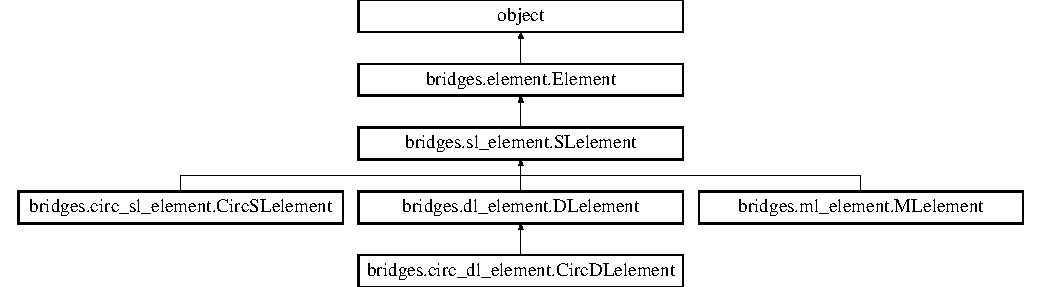
\includegraphics[height=3.856750cm]{classbridges_1_1sl__element_1_1_s_lelement}
\end{center}
\end{figure}
\doxysubsection*{Public Member Functions}
\begin{DoxyCompactItemize}
\item 
def \mbox{\hyperlink{classbridges_1_1sl__element_1_1_s_lelement_ad2d298e03cbda62f6c8afac630179f16}{\+\_\+\+\_\+init\+\_\+\+\_\+}} (self, e=None, \mbox{\hyperlink{classbridges_1_1element_1_1_element_a97551dbb005cd5d1f13b65461290c6e3}{label}}=None, \mbox{\hyperlink{classbridges_1_1sl__element_1_1_s_lelement_a4fa8e9321dd2ce726da047ddc64adabf}{next}}=None)
\begin{DoxyCompactList}\small\item\em This constructor creates an \mbox{\hyperlink{classbridges_1_1sl__element_1_1_s_lelement}{S\+Lelement}} object and sets the next pointer to null. \end{DoxyCompactList}\item 
def \mbox{\hyperlink{classbridges_1_1sl__element_1_1_s_lelement_aa39835634a95d832d092dd3c057a49cf}{get\+\_\+data\+\_\+structure\+\_\+type}} (self)
\item 
def \mbox{\hyperlink{classbridges_1_1sl__element_1_1_s_lelement_ae15a5fe6db55b10f3fe09f8039291960}{get\+\_\+next}} (self)
\begin{DoxyCompactList}\small\item\em Retrieves the element following this element. \end{DoxyCompactList}\item 
def \mbox{\hyperlink{classbridges_1_1sl__element_1_1_s_lelement_a0b39165322e4349714219077b13ac35a}{get\+\_\+value}} (self)
\begin{DoxyCompactList}\small\item\em Retrieves the value in the \mbox{\hyperlink{classbridges_1_1sl__element_1_1_s_lelement}{S\+Lelement}}. \end{DoxyCompactList}\item 
def \mbox{\hyperlink{classbridges_1_1sl__element_1_1_s_lelement_a607068c196b64971d16e4bf169b85cdd}{set\+\_\+next}} (self, \mbox{\hyperlink{classbridges_1_1sl__element_1_1_s_lelement_a4fa8e9321dd2ce726da047ddc64adabf}{next}})
\begin{DoxyCompactList}\small\item\em Sets the element to point to the next \mbox{\hyperlink{classbridges_1_1sl__element_1_1_s_lelement}{S\+Lelement}}. \end{DoxyCompactList}\item 
def \mbox{\hyperlink{classbridges_1_1sl__element_1_1_s_lelement_a985f205ebff285c3bc72d342adf1308e}{\+\_\+\+\_\+str\+\_\+\+\_\+}} (self)
\item 
def \mbox{\hyperlink{classbridges_1_1sl__element_1_1_s_lelement_af1d3039c3597ce0345d1cd973711714f}{get\+\_\+data\+\_\+structure\+\_\+representation}} (self)
\begin{DoxyCompactList}\small\item\em Get the J\+S\+ON representation of the the data structure. \end{DoxyCompactList}\item 
def \mbox{\hyperlink{classbridges_1_1sl__element_1_1_s_lelement_ad3b94c8e7540aca841e6306c190e1be1}{get\+\_\+list\+\_\+elements}} (self, nodes)
\begin{DoxyCompactList}\small\item\em Get the elements of the list. \end{DoxyCompactList}\end{DoxyCompactItemize}
\doxysubsection*{Public Attributes}
\begin{DoxyCompactItemize}
\item 
\mbox{\hyperlink{classbridges_1_1sl__element_1_1_s_lelement_a4fa8e9321dd2ce726da047ddc64adabf}{next}}
\end{DoxyCompactItemize}
\doxysubsection*{Additional Inherited Members}


\doxysubsection{Detailed Description}
This class can be used to instantiate Singly Linked Elements. 

This class extends Element and takes a generic parameter $<$\+E$>$ representing application specific data. This element forms the basic building block for singly linked lists. Singly linked elements have a field pointing to the next element along the list.

\begin{DoxyVerb}Elements contain a visualizer (ElementVisualizer) object for setting visual
attributes (color, shape, opacity, size), necessary for displaying them in a
web browser.

Elements also have a LinkVisualizer object, that is used when they are linked to
another element, appropriate for setting link attributes, for instance, between
the current element and its next element.
\end{DoxyVerb}
 

\doxysubsection{Constructor \& Destructor Documentation}
\mbox{\Hypertarget{classbridges_1_1sl__element_1_1_s_lelement_ad2d298e03cbda62f6c8afac630179f16}\label{classbridges_1_1sl__element_1_1_s_lelement_ad2d298e03cbda62f6c8afac630179f16}} 
\index{bridges.sl\_element.SLelement@{bridges.sl\_element.SLelement}!\_\_init\_\_@{\_\_init\_\_}}
\index{\_\_init\_\_@{\_\_init\_\_}!bridges.sl\_element.SLelement@{bridges.sl\_element.SLelement}}
\doxysubsubsection{\texorpdfstring{\_\_init\_\_()}{\_\_init\_\_()}}
{\footnotesize\ttfamily def bridges.\+sl\+\_\+element.\+S\+Lelement.\+\_\+\+\_\+init\+\_\+\+\_\+ (\begin{DoxyParamCaption}\item[{}]{self,  }\item[{}]{e = {\ttfamily None},  }\item[{}]{label = {\ttfamily None},  }\item[{}]{next = {\ttfamily None} }\end{DoxyParamCaption})}



This constructor creates an \mbox{\hyperlink{classbridges_1_1sl__element_1_1_s_lelement}{S\+Lelement}} object and sets the next pointer to null. 


\begin{DoxyParams}{Parameters}
{\em label} & -\/ the label of \mbox{\hyperlink{classbridges_1_1sl__element_1_1_s_lelement}{S\+Lelement}} that shows up on the bridges visualization \\
\hline
{\em e} & -\/ the generic object that this \mbox{\hyperlink{classbridges_1_1sl__element_1_1_s_lelement}{S\+Lelement}} will hold \\
\hline
{\em next} & -\/ the element that should be assigned to the next pointer \\
\hline
\end{DoxyParams}


Reimplemented from \mbox{\hyperlink{classbridges_1_1element_1_1_element_a31faee32348c800860f32876b6865ad0}{bridges.\+element.\+Element}}.



Reimplemented in \mbox{\hyperlink{classbridges_1_1circ__sl__element_1_1_circ_s_lelement_a691e2db0878e32d0298204685a120268}{bridges.\+circ\+\_\+sl\+\_\+element.\+Circ\+S\+Lelement}}.



\doxysubsection{Member Function Documentation}
\mbox{\Hypertarget{classbridges_1_1sl__element_1_1_s_lelement_a985f205ebff285c3bc72d342adf1308e}\label{classbridges_1_1sl__element_1_1_s_lelement_a985f205ebff285c3bc72d342adf1308e}} 
\index{bridges.sl\_element.SLelement@{bridges.sl\_element.SLelement}!\_\_str\_\_@{\_\_str\_\_}}
\index{\_\_str\_\_@{\_\_str\_\_}!bridges.sl\_element.SLelement@{bridges.sl\_element.SLelement}}
\doxysubsubsection{\texorpdfstring{\_\_str\_\_()}{\_\_str\_\_()}}
{\footnotesize\ttfamily def bridges.\+sl\+\_\+element.\+S\+Lelement.\+\_\+\+\_\+str\+\_\+\+\_\+ (\begin{DoxyParamCaption}\item[{}]{self }\end{DoxyParamCaption})}



Reimplemented from \mbox{\hyperlink{classbridges_1_1element_1_1_element_a92a94c7f36d8cfb5db5435013556519a}{bridges.\+element.\+Element}}.



Reimplemented in \mbox{\hyperlink{classbridges_1_1circ__sl__element_1_1_circ_s_lelement_af43d07b196276fea57e9d43caf9f6c98}{bridges.\+circ\+\_\+sl\+\_\+element.\+Circ\+S\+Lelement}}.

\mbox{\Hypertarget{classbridges_1_1sl__element_1_1_s_lelement_af1d3039c3597ce0345d1cd973711714f}\label{classbridges_1_1sl__element_1_1_s_lelement_af1d3039c3597ce0345d1cd973711714f}} 
\index{bridges.sl\_element.SLelement@{bridges.sl\_element.SLelement}!get\_data\_structure\_representation@{get\_data\_structure\_representation}}
\index{get\_data\_structure\_representation@{get\_data\_structure\_representation}!bridges.sl\_element.SLelement@{bridges.sl\_element.SLelement}}
\doxysubsubsection{\texorpdfstring{get\_data\_structure\_representation()}{get\_data\_structure\_representation()}}
{\footnotesize\ttfamily def bridges.\+sl\+\_\+element.\+S\+Lelement.\+get\+\_\+data\+\_\+structure\+\_\+representation (\begin{DoxyParamCaption}\item[{}]{self }\end{DoxyParamCaption})}



Get the J\+S\+ON representation of the the data structure. 



Reimplemented in \mbox{\hyperlink{classbridges_1_1ml__element_1_1_m_lelement_a7d176b966746a889f9234d4a76b99c0c}{bridges.\+ml\+\_\+element.\+M\+Lelement}}, and \mbox{\hyperlink{classbridges_1_1dl__element_1_1_d_lelement_abcae653ca8e9590c594910bad148ddf2}{bridges.\+dl\+\_\+element.\+D\+Lelement}}.

\mbox{\Hypertarget{classbridges_1_1sl__element_1_1_s_lelement_aa39835634a95d832d092dd3c057a49cf}\label{classbridges_1_1sl__element_1_1_s_lelement_aa39835634a95d832d092dd3c057a49cf}} 
\index{bridges.sl\_element.SLelement@{bridges.sl\_element.SLelement}!get\_data\_structure\_type@{get\_data\_structure\_type}}
\index{get\_data\_structure\_type@{get\_data\_structure\_type}!bridges.sl\_element.SLelement@{bridges.sl\_element.SLelement}}
\doxysubsubsection{\texorpdfstring{get\_data\_structure\_type()}{get\_data\_structure\_type()}}
{\footnotesize\ttfamily def bridges.\+sl\+\_\+element.\+S\+Lelement.\+get\+\_\+data\+\_\+structure\+\_\+type (\begin{DoxyParamCaption}\item[{}]{self }\end{DoxyParamCaption})}

\begin{DoxyVerb}This method gets the data structure type

@return  The date structure type as a string
\end{DoxyVerb}
 

Reimplemented from \mbox{\hyperlink{classbridges_1_1element_1_1_element_a87b8c79123d20eb2af48ae4e4f1bcf32}{bridges.\+element.\+Element}}.



Reimplemented in \mbox{\hyperlink{classbridges_1_1ml__element_1_1_m_lelement_a97693d616263a8ee59b066829e8ce7e8}{bridges.\+ml\+\_\+element.\+M\+Lelement}}, \mbox{\hyperlink{classbridges_1_1circ__dl__element_1_1_circ_d_lelement_ac33a5699a662730bb6f292654e6896dc}{bridges.\+circ\+\_\+dl\+\_\+element.\+Circ\+D\+Lelement}}, \mbox{\hyperlink{classbridges_1_1circ__sl__element_1_1_circ_s_lelement_a82b1dbb8592c943eb68161ee60ac3492}{bridges.\+circ\+\_\+sl\+\_\+element.\+Circ\+S\+Lelement}}, and \mbox{\hyperlink{classbridges_1_1dl__element_1_1_d_lelement_a5fb177ed67b75e606ac303f7a972d301}{bridges.\+dl\+\_\+element.\+D\+Lelement}}.

\mbox{\Hypertarget{classbridges_1_1sl__element_1_1_s_lelement_ad3b94c8e7540aca841e6306c190e1be1}\label{classbridges_1_1sl__element_1_1_s_lelement_ad3b94c8e7540aca841e6306c190e1be1}} 
\index{bridges.sl\_element.SLelement@{bridges.sl\_element.SLelement}!get\_list\_elements@{get\_list\_elements}}
\index{get\_list\_elements@{get\_list\_elements}!bridges.sl\_element.SLelement@{bridges.sl\_element.SLelement}}
\doxysubsubsection{\texorpdfstring{get\_list\_elements()}{get\_list\_elements()}}
{\footnotesize\ttfamily def bridges.\+sl\+\_\+element.\+S\+Lelement.\+get\+\_\+list\+\_\+elements (\begin{DoxyParamCaption}\item[{}]{self,  }\item[{}]{nodes }\end{DoxyParamCaption})}



Get the elements of the list. 


\begin{DoxyParams}{Parameters}
{\em nodes} & a vector of the ndoes in the list \\
\hline
\end{DoxyParams}


Reimplemented in \mbox{\hyperlink{classbridges_1_1ml__element_1_1_m_lelement_a3996cd2cec7c3978437392eba2ef66eb}{bridges.\+ml\+\_\+element.\+M\+Lelement}}.

\mbox{\Hypertarget{classbridges_1_1sl__element_1_1_s_lelement_ae15a5fe6db55b10f3fe09f8039291960}\label{classbridges_1_1sl__element_1_1_s_lelement_ae15a5fe6db55b10f3fe09f8039291960}} 
\index{bridges.sl\_element.SLelement@{bridges.sl\_element.SLelement}!get\_next@{get\_next}}
\index{get\_next@{get\_next}!bridges.sl\_element.SLelement@{bridges.sl\_element.SLelement}}
\doxysubsubsection{\texorpdfstring{get\_next()}{get\_next()}}
{\footnotesize\ttfamily def bridges.\+sl\+\_\+element.\+S\+Lelement.\+get\+\_\+next (\begin{DoxyParamCaption}\item[{}]{self }\end{DoxyParamCaption})}



Retrieves the element following this element. 

\begin{DoxyReturn}{Returns}
-\/ \mbox{\hyperlink{classbridges_1_1sl__element_1_1_s_lelement}{S\+Lelement}} assigned to next 
\end{DoxyReturn}


Reimplemented in \mbox{\hyperlink{classbridges_1_1ml__element_1_1_m_lelement_aca0cc01e2041a3d283a3e1ceca3050da}{bridges.\+ml\+\_\+element.\+M\+Lelement}}, \mbox{\hyperlink{classbridges_1_1circ__dl__element_1_1_circ_d_lelement_a7a0432dd9694cb389db12a0027af04cc}{bridges.\+circ\+\_\+dl\+\_\+element.\+Circ\+D\+Lelement}}, \mbox{\hyperlink{classbridges_1_1circ__sl__element_1_1_circ_s_lelement_acd9041487068ad5b8e9b68dfcdff4829}{bridges.\+circ\+\_\+sl\+\_\+element.\+Circ\+S\+Lelement}}, and \mbox{\hyperlink{classbridges_1_1dl__element_1_1_d_lelement_a268ae3965f0cba4a801e73f61b7c9fcc}{bridges.\+dl\+\_\+element.\+D\+Lelement}}.

\mbox{\Hypertarget{classbridges_1_1sl__element_1_1_s_lelement_a0b39165322e4349714219077b13ac35a}\label{classbridges_1_1sl__element_1_1_s_lelement_a0b39165322e4349714219077b13ac35a}} 
\index{bridges.sl\_element.SLelement@{bridges.sl\_element.SLelement}!get\_value@{get\_value}}
\index{get\_value@{get\_value}!bridges.sl\_element.SLelement@{bridges.sl\_element.SLelement}}
\doxysubsubsection{\texorpdfstring{get\_value()}{get\_value()}}
{\footnotesize\ttfamily def bridges.\+sl\+\_\+element.\+S\+Lelement.\+get\+\_\+value (\begin{DoxyParamCaption}\item[{}]{self }\end{DoxyParamCaption})}



Retrieves the value in the \mbox{\hyperlink{classbridges_1_1sl__element_1_1_s_lelement}{S\+Lelement}}. 

\begin{DoxyReturn}{Returns}
-\/ S\+L\+Element value held 
\end{DoxyReturn}


Reimplemented from \mbox{\hyperlink{classbridges_1_1element_1_1_element_aafcdc6c1661ddbf28e664b69c72ed5a4}{bridges.\+element.\+Element}}.

\mbox{\Hypertarget{classbridges_1_1sl__element_1_1_s_lelement_a607068c196b64971d16e4bf169b85cdd}\label{classbridges_1_1sl__element_1_1_s_lelement_a607068c196b64971d16e4bf169b85cdd}} 
\index{bridges.sl\_element.SLelement@{bridges.sl\_element.SLelement}!set\_next@{set\_next}}
\index{set\_next@{set\_next}!bridges.sl\_element.SLelement@{bridges.sl\_element.SLelement}}
\doxysubsubsection{\texorpdfstring{set\_next()}{set\_next()}}
{\footnotesize\ttfamily def bridges.\+sl\+\_\+element.\+S\+Lelement.\+set\+\_\+next (\begin{DoxyParamCaption}\item[{}]{self,  }\item[{}]{next }\end{DoxyParamCaption})}



Sets the element to point to the next \mbox{\hyperlink{classbridges_1_1sl__element_1_1_s_lelement}{S\+Lelement}}. 


\begin{DoxyParams}{Parameters}
{\em next} & -\/ \mbox{\hyperlink{classbridges_1_1sl__element_1_1_s_lelement}{S\+Lelement}} that should be assigned to the next pointer \\
\hline
\end{DoxyParams}


\doxysubsection{Member Data Documentation}
\mbox{\Hypertarget{classbridges_1_1sl__element_1_1_s_lelement_a4fa8e9321dd2ce726da047ddc64adabf}\label{classbridges_1_1sl__element_1_1_s_lelement_a4fa8e9321dd2ce726da047ddc64adabf}} 
\index{bridges.sl\_element.SLelement@{bridges.sl\_element.SLelement}!next@{next}}
\index{next@{next}!bridges.sl\_element.SLelement@{bridges.sl\_element.SLelement}}
\doxysubsubsection{\texorpdfstring{next}{next}}
{\footnotesize\ttfamily bridges.\+sl\+\_\+element.\+S\+Lelement.\+next}



The documentation for this class was generated from the following file\+:\begin{DoxyCompactItemize}
\item 
/\+Users/kalpathi/gr/bridges/client/python/bridges/\mbox{\hyperlink{sl__element_8py}{sl\+\_\+element.\+py}}\end{DoxyCompactItemize}

\hypertarget{classbridges_1_1tree__element_1_1_tree_element}{}\section{bridges.\+tree\+\_\+element.\+Tree\+Element Class Reference}
\label{classbridges_1_1tree__element_1_1_tree_element}\index{bridges.\+tree\+\_\+element.\+Tree\+Element@{bridges.\+tree\+\_\+element.\+Tree\+Element}}


This class extends Element to represent general trees with arbitrary number of children.  


Inheritance diagram for bridges.\+tree\+\_\+element.\+Tree\+Element\+:\begin{figure}[H]
\begin{center}
\leavevmode
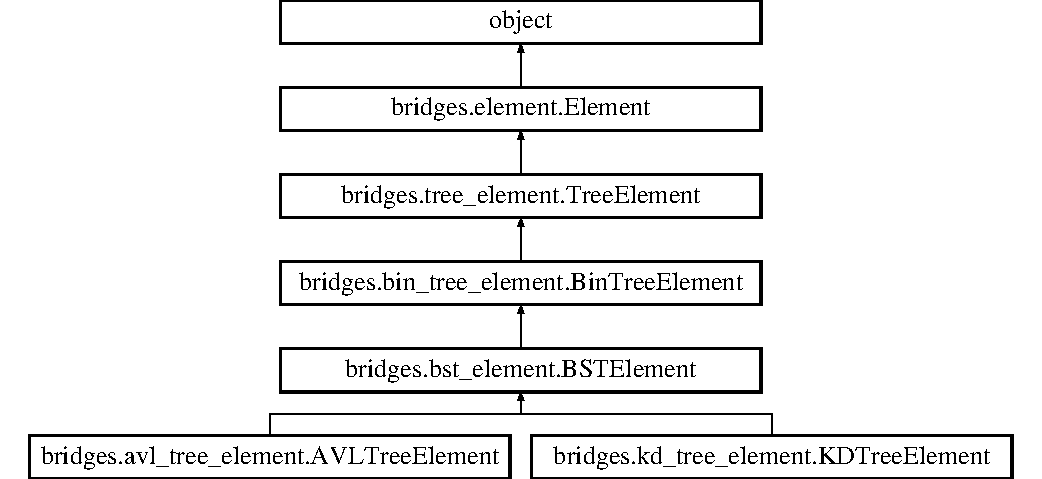
\includegraphics[height=6.000000cm]{classbridges_1_1tree__element_1_1_tree_element}
\end{center}
\end{figure}
\subsection*{Public Member Functions}
\begin{DoxyCompactItemize}
\item 
def \hyperlink{classbridges_1_1tree__element_1_1_tree_element_a72adc790d9719f265d949f7bf4e8f056}{\+\_\+\+\_\+init\+\_\+\+\_\+}
\begin{DoxyCompactList}\small\item\em Constructs an \hyperlink{classbridges_1_1tree__element_1_1_tree_element}{Tree\+Element} set to null. \end{DoxyCompactList}\item 
def \hyperlink{classbridges_1_1tree__element_1_1_tree_element_aeefaf309c1271b2e7272cf63be496457}{get\+\_\+data\+\_\+structure\+\_\+type} (self)
\begin{DoxyCompactList}\small\item\em This method gets the data structure type. \end{DoxyCompactList}\item 
def \hyperlink{classbridges_1_1tree__element_1_1_tree_element_a7a5933a3de19a896712389dda41a4452}{add\+\_\+child} (self, child)
\begin{DoxyCompactList}\small\item\em Adds a child to the node. \end{DoxyCompactList}\item 
def \hyperlink{classbridges_1_1tree__element_1_1_tree_element_a5d0c6335324d675a6c0329dad72fca4d}{get\+\_\+number\+\_\+of\+\_\+children} (self)
\begin{DoxyCompactList}\small\item\em Returns the number of children at this node. \end{DoxyCompactList}\item 
def \hyperlink{classbridges_1_1tree__element_1_1_tree_element_aa77f48683b351512dcdf6ec2e90d9a91}{set\+\_\+child} (self, index, child)
\begin{DoxyCompactList}\small\item\em adds a child to the node -\/ will be added at the next open position \end{DoxyCompactList}\item 
def \hyperlink{classbridges_1_1tree__element_1_1_tree_element_ac216f30d22883aa58867de96e03444f1}{get\+\_\+child} (self, index)
\begin{DoxyCompactList}\small\item\em gets a child at a particular index \end{DoxyCompactList}\item 
def \hyperlink{classbridges_1_1tree__element_1_1_tree_element_ac578f7744d2553c91962b01b57b0e783}{get\+\_\+data\+\_\+structure\+\_\+representation} (self)
\begin{DoxyCompactList}\small\item\em Get hierarchical J\+S\+O\+N of the tree representation. \end{DoxyCompactList}\item 
def \hyperlink{classbridges_1_1tree__element_1_1_tree_element_a6b8fa6eb2b2ffb015c64955575057d3a}{pre\+\_\+order} (self, root)
\begin{DoxyCompactList}\small\item\em Use a preorder traversal to directly extract a hierarchical J\+S\+O\+N representation of the tree. \end{DoxyCompactList}\end{DoxyCompactItemize}
\subsection*{Public Attributes}
\begin{DoxyCompactItemize}
\item 
\hyperlink{classbridges_1_1tree__element_1_1_tree_element_a09e0e8ad32395e004b6b2d12c39ce390}{children}
\end{DoxyCompactItemize}
\subsection*{Static Public Attributes}
\begin{DoxyCompactItemize}
\item 
list \hyperlink{classbridges_1_1tree__element_1_1_tree_element_a620604f4f3571fdf8e3e94c193b86948}{children} = \mbox{[}$\,$\mbox{]}
\item 
string \hyperlink{classbridges_1_1tree__element_1_1_tree_element_aa5a4d14f38ceb896a85ef0b703d6995a}{Q\+U\+O\+T\+E} = \char`\"{}\textbackslash{}\char`\"{}\char`\"{}
\item 
string \hyperlink{classbridges_1_1tree__element_1_1_tree_element_a427a0eaaae4cf421dc0353ca8f4047d2}{C\+O\+M\+M\+A} = \char`\"{},\char`\"{}
\item 
string \hyperlink{classbridges_1_1tree__element_1_1_tree_element_a1ece84d898aec2a9340f45e52ace2313}{C\+O\+L\+O\+N} = \char`\"{}\+:\char`\"{}
\item 
string \hyperlink{classbridges_1_1tree__element_1_1_tree_element_abff31b93e3dfe4c3089d3a14abeede86}{O\+P\+E\+N\+\_\+\+C\+U\+R\+L\+Y} = \char`\"{}\{\char`\"{}
\item 
string \hyperlink{classbridges_1_1tree__element_1_1_tree_element_a30e6828805446c2c86423c334c81c981}{C\+L\+O\+S\+E\+\_\+\+C\+U\+R\+L\+Y} = \char`\"{}\}\char`\"{}
\item 
string \hyperlink{classbridges_1_1tree__element_1_1_tree_element_a09d8d27767e40f3b84a8395123cfa15a}{O\+P\+E\+N\+\_\+\+P\+A\+R\+E\+N} = \char`\"{}(\char`\"{}
\item 
string \hyperlink{classbridges_1_1tree__element_1_1_tree_element_ae6264b1611ca448a64e3ef3ac4baf8da}{C\+L\+O\+S\+E\+\_\+\+P\+A\+R\+E\+N} = \char`\"{})\char`\"{}
\item 
string \hyperlink{classbridges_1_1tree__element_1_1_tree_element_a61cd10ef5adf34b1aa56a6be855fb2c9}{O\+P\+E\+N\+\_\+\+B\+O\+X} = \char`\"{}\mbox{[}\char`\"{}
\item 
string \hyperlink{classbridges_1_1tree__element_1_1_tree_element_a35214b444048a585452a8451cd23c802}{C\+L\+O\+S\+E\+\_\+\+B\+O\+X} = \char`\"{}\mbox{]}\char`\"{}
\end{DoxyCompactItemize}


\subsection{Detailed Description}
This class extends Element to represent general trees with arbitrary number of children. 

\hyperlink{classbridges_1_1tree__element_1_1_tree_element}{Tree\+Element} nodes can have an arbitrary number of child nodes(held in in a vector in the order in which they were added). The visualization of trees assumes that the children are drawn in order from left to right.

Tree Elements have labels (string) that are displayed on the visualization. Elements take an generic object E as a user defined parameter, which can be any native type or object.

Elements contain a visualizer (Element\+Visualizer) object for setting visual attributes (color, shape, opacity, size), necessary for displaying them in a web browser.

Elements also have a Link\+Visualizer object that is used when they are linked to another element, appropriate for setting link attributes, between parent and child nodes.

\begin{DoxyAuthor}{Author}
Matthew Mc\+Quaigue 
\end{DoxyAuthor}


\subsection{Constructor \& Destructor Documentation}
\hypertarget{classbridges_1_1tree__element_1_1_tree_element_a72adc790d9719f265d949f7bf4e8f056}{}\index{bridges\+::tree\+\_\+element\+::\+Tree\+Element@{bridges\+::tree\+\_\+element\+::\+Tree\+Element}!\+\_\+\+\_\+init\+\_\+\+\_\+@{\+\_\+\+\_\+init\+\_\+\+\_\+}}
\index{\+\_\+\+\_\+init\+\_\+\+\_\+@{\+\_\+\+\_\+init\+\_\+\+\_\+}!bridges\+::tree\+\_\+element\+::\+Tree\+Element@{bridges\+::tree\+\_\+element\+::\+Tree\+Element}}
\subsubsection[{\+\_\+\+\_\+init\+\_\+\+\_\+}]{\setlength{\rightskip}{0pt plus 5cm}def bridges.\+tree\+\_\+element.\+Tree\+Element.\+\_\+\+\_\+init\+\_\+\+\_\+ (
\begin{DoxyParamCaption}
\item[{}]{self, }
\item[{}]{label = {\ttfamily None}, }
\item[{}]{e = {\ttfamily None}, }
\item[{}]{left = {\ttfamily None}, }
\item[{}]{right = {\ttfamily None}}
\end{DoxyParamCaption}
)}\label{classbridges_1_1tree__element_1_1_tree_element_a72adc790d9719f265d949f7bf4e8f056}


Constructs an \hyperlink{classbridges_1_1tree__element_1_1_tree_element}{Tree\+Element} set to null. 


\begin{DoxyParams}{Parameters}
{\em e} & the generic object that \hyperlink{classbridges_1_1tree__element_1_1_tree_element}{Tree\+Element} will hold \\
\hline
{\em label} & the label of \hyperlink{classbridges_1_1tree__element_1_1_tree_element}{Tree\+Element} that shows up on the bridges \\
\hline
{\em left} & the \hyperlink{classbridges_1_1tree__element_1_1_tree_element}{Tree\+Element} to be assigned to the child 0 \\
\hline
{\em right} & the \hyperlink{classbridges_1_1tree__element_1_1_tree_element}{Tree\+Element} to be assigned to the child 1 \\
\hline
\end{DoxyParams}


\subsection{Member Function Documentation}
\hypertarget{classbridges_1_1tree__element_1_1_tree_element_a7a5933a3de19a896712389dda41a4452}{}\index{bridges\+::tree\+\_\+element\+::\+Tree\+Element@{bridges\+::tree\+\_\+element\+::\+Tree\+Element}!add\+\_\+child@{add\+\_\+child}}
\index{add\+\_\+child@{add\+\_\+child}!bridges\+::tree\+\_\+element\+::\+Tree\+Element@{bridges\+::tree\+\_\+element\+::\+Tree\+Element}}
\subsubsection[{add\+\_\+child(self, child)}]{\setlength{\rightskip}{0pt plus 5cm}def bridges.\+tree\+\_\+element.\+Tree\+Element.\+add\+\_\+child (
\begin{DoxyParamCaption}
\item[{}]{self, }
\item[{}]{child}
\end{DoxyParamCaption}
)}\label{classbridges_1_1tree__element_1_1_tree_element_a7a5933a3de19a896712389dda41a4452}


Adds a child to the node. 

\hypertarget{classbridges_1_1tree__element_1_1_tree_element_ac216f30d22883aa58867de96e03444f1}{}\index{bridges\+::tree\+\_\+element\+::\+Tree\+Element@{bridges\+::tree\+\_\+element\+::\+Tree\+Element}!get\+\_\+child@{get\+\_\+child}}
\index{get\+\_\+child@{get\+\_\+child}!bridges\+::tree\+\_\+element\+::\+Tree\+Element@{bridges\+::tree\+\_\+element\+::\+Tree\+Element}}
\subsubsection[{get\+\_\+child(self, index)}]{\setlength{\rightskip}{0pt plus 5cm}def bridges.\+tree\+\_\+element.\+Tree\+Element.\+get\+\_\+child (
\begin{DoxyParamCaption}
\item[{}]{self, }
\item[{}]{index}
\end{DoxyParamCaption}
)}\label{classbridges_1_1tree__element_1_1_tree_element_ac216f30d22883aa58867de96e03444f1}


gets a child at a particular index 


\begin{DoxyParams}{Parameters}
{\em index} & into the list of children\\
\hline
\end{DoxyParams}
\begin{DoxyReturn}{Returns}
child to be returned 
\end{DoxyReturn}
\hypertarget{classbridges_1_1tree__element_1_1_tree_element_ac578f7744d2553c91962b01b57b0e783}{}\index{bridges\+::tree\+\_\+element\+::\+Tree\+Element@{bridges\+::tree\+\_\+element\+::\+Tree\+Element}!get\+\_\+data\+\_\+structure\+\_\+representation@{get\+\_\+data\+\_\+structure\+\_\+representation}}
\index{get\+\_\+data\+\_\+structure\+\_\+representation@{get\+\_\+data\+\_\+structure\+\_\+representation}!bridges\+::tree\+\_\+element\+::\+Tree\+Element@{bridges\+::tree\+\_\+element\+::\+Tree\+Element}}
\subsubsection[{get\+\_\+data\+\_\+structure\+\_\+representation(self)}]{\setlength{\rightskip}{0pt plus 5cm}def bridges.\+tree\+\_\+element.\+Tree\+Element.\+get\+\_\+data\+\_\+structure\+\_\+representation (
\begin{DoxyParamCaption}
\item[{}]{self}
\end{DoxyParamCaption}
)}\label{classbridges_1_1tree__element_1_1_tree_element_ac578f7744d2553c91962b01b57b0e783}


Get hierarchical J\+S\+O\+N of the tree representation. 

\begin{DoxyReturn}{Returns}
the J\+S\+O\+N string 
\end{DoxyReturn}
\hypertarget{classbridges_1_1tree__element_1_1_tree_element_aeefaf309c1271b2e7272cf63be496457}{}\index{bridges\+::tree\+\_\+element\+::\+Tree\+Element@{bridges\+::tree\+\_\+element\+::\+Tree\+Element}!get\+\_\+data\+\_\+structure\+\_\+type@{get\+\_\+data\+\_\+structure\+\_\+type}}
\index{get\+\_\+data\+\_\+structure\+\_\+type@{get\+\_\+data\+\_\+structure\+\_\+type}!bridges\+::tree\+\_\+element\+::\+Tree\+Element@{bridges\+::tree\+\_\+element\+::\+Tree\+Element}}
\subsubsection[{get\+\_\+data\+\_\+structure\+\_\+type(self)}]{\setlength{\rightskip}{0pt plus 5cm}def bridges.\+tree\+\_\+element.\+Tree\+Element.\+get\+\_\+data\+\_\+structure\+\_\+type (
\begin{DoxyParamCaption}
\item[{}]{self}
\end{DoxyParamCaption}
)}\label{classbridges_1_1tree__element_1_1_tree_element_aeefaf309c1271b2e7272cf63be496457}


This method gets the data structure type. 

\begin{DoxyReturn}{Returns}
The date structure type as a string 
\end{DoxyReturn}
\hypertarget{classbridges_1_1tree__element_1_1_tree_element_a5d0c6335324d675a6c0329dad72fca4d}{}\index{bridges\+::tree\+\_\+element\+::\+Tree\+Element@{bridges\+::tree\+\_\+element\+::\+Tree\+Element}!get\+\_\+number\+\_\+of\+\_\+children@{get\+\_\+number\+\_\+of\+\_\+children}}
\index{get\+\_\+number\+\_\+of\+\_\+children@{get\+\_\+number\+\_\+of\+\_\+children}!bridges\+::tree\+\_\+element\+::\+Tree\+Element@{bridges\+::tree\+\_\+element\+::\+Tree\+Element}}
\subsubsection[{get\+\_\+number\+\_\+of\+\_\+children(self)}]{\setlength{\rightskip}{0pt plus 5cm}def bridges.\+tree\+\_\+element.\+Tree\+Element.\+get\+\_\+number\+\_\+of\+\_\+children (
\begin{DoxyParamCaption}
\item[{}]{self}
\end{DoxyParamCaption}
)}\label{classbridges_1_1tree__element_1_1_tree_element_a5d0c6335324d675a6c0329dad72fca4d}


Returns the number of children at this node. 

\begin{DoxyReturn}{Returns}
number of children 
\end{DoxyReturn}
\hypertarget{classbridges_1_1tree__element_1_1_tree_element_a6b8fa6eb2b2ffb015c64955575057d3a}{}\index{bridges\+::tree\+\_\+element\+::\+Tree\+Element@{bridges\+::tree\+\_\+element\+::\+Tree\+Element}!pre\+\_\+order@{pre\+\_\+order}}
\index{pre\+\_\+order@{pre\+\_\+order}!bridges\+::tree\+\_\+element\+::\+Tree\+Element@{bridges\+::tree\+\_\+element\+::\+Tree\+Element}}
\subsubsection[{pre\+\_\+order(self, root)}]{\setlength{\rightskip}{0pt plus 5cm}def bridges.\+tree\+\_\+element.\+Tree\+Element.\+pre\+\_\+order (
\begin{DoxyParamCaption}
\item[{}]{self, }
\item[{}]{root}
\end{DoxyParamCaption}
)}\label{classbridges_1_1tree__element_1_1_tree_element_a6b8fa6eb2b2ffb015c64955575057d3a}


Use a preorder traversal to directly extract a hierarchical J\+S\+O\+N representation of the tree. 

\hypertarget{classbridges_1_1tree__element_1_1_tree_element_aa77f48683b351512dcdf6ec2e90d9a91}{}\index{bridges\+::tree\+\_\+element\+::\+Tree\+Element@{bridges\+::tree\+\_\+element\+::\+Tree\+Element}!set\+\_\+child@{set\+\_\+child}}
\index{set\+\_\+child@{set\+\_\+child}!bridges\+::tree\+\_\+element\+::\+Tree\+Element@{bridges\+::tree\+\_\+element\+::\+Tree\+Element}}
\subsubsection[{set\+\_\+child(self, index, child)}]{\setlength{\rightskip}{0pt plus 5cm}def bridges.\+tree\+\_\+element.\+Tree\+Element.\+set\+\_\+child (
\begin{DoxyParamCaption}
\item[{}]{self, }
\item[{}]{index, }
\item[{}]{child}
\end{DoxyParamCaption}
)}\label{classbridges_1_1tree__element_1_1_tree_element_aa77f48683b351512dcdf6ec2e90d9a91}


adds a child to the node -\/ will be added at the next open position 


\begin{DoxyParams}{Parameters}
{\em child} & to be added\\
\hline
\end{DoxyParams}
\begin{DoxyReturn}{Returns}
none 
\end{DoxyReturn}


\subsection{Member Data Documentation}
\hypertarget{classbridges_1_1tree__element_1_1_tree_element_a620604f4f3571fdf8e3e94c193b86948}{}\index{bridges\+::tree\+\_\+element\+::\+Tree\+Element@{bridges\+::tree\+\_\+element\+::\+Tree\+Element}!children@{children}}
\index{children@{children}!bridges\+::tree\+\_\+element\+::\+Tree\+Element@{bridges\+::tree\+\_\+element\+::\+Tree\+Element}}
\subsubsection[{children}]{\setlength{\rightskip}{0pt plus 5cm}list bridges.\+tree\+\_\+element.\+Tree\+Element.\+children = \mbox{[}$\,$\mbox{]}\hspace{0.3cm}{\ttfamily [static]}}\label{classbridges_1_1tree__element_1_1_tree_element_a620604f4f3571fdf8e3e94c193b86948}
\hypertarget{classbridges_1_1tree__element_1_1_tree_element_a09e0e8ad32395e004b6b2d12c39ce390}{}\index{bridges\+::tree\+\_\+element\+::\+Tree\+Element@{bridges\+::tree\+\_\+element\+::\+Tree\+Element}!children@{children}}
\index{children@{children}!bridges\+::tree\+\_\+element\+::\+Tree\+Element@{bridges\+::tree\+\_\+element\+::\+Tree\+Element}}
\subsubsection[{children}]{\setlength{\rightskip}{0pt plus 5cm}bridges.\+tree\+\_\+element.\+Tree\+Element.\+children}\label{classbridges_1_1tree__element_1_1_tree_element_a09e0e8ad32395e004b6b2d12c39ce390}
\hypertarget{classbridges_1_1tree__element_1_1_tree_element_a35214b444048a585452a8451cd23c802}{}\index{bridges\+::tree\+\_\+element\+::\+Tree\+Element@{bridges\+::tree\+\_\+element\+::\+Tree\+Element}!C\+L\+O\+S\+E\+\_\+\+B\+O\+X@{C\+L\+O\+S\+E\+\_\+\+B\+O\+X}}
\index{C\+L\+O\+S\+E\+\_\+\+B\+O\+X@{C\+L\+O\+S\+E\+\_\+\+B\+O\+X}!bridges\+::tree\+\_\+element\+::\+Tree\+Element@{bridges\+::tree\+\_\+element\+::\+Tree\+Element}}
\subsubsection[{C\+L\+O\+S\+E\+\_\+\+B\+O\+X}]{\setlength{\rightskip}{0pt plus 5cm}string bridges.\+tree\+\_\+element.\+Tree\+Element.\+C\+L\+O\+S\+E\+\_\+\+B\+O\+X = \char`\"{}\mbox{]}\char`\"{}\hspace{0.3cm}{\ttfamily [static]}}\label{classbridges_1_1tree__element_1_1_tree_element_a35214b444048a585452a8451cd23c802}
\hypertarget{classbridges_1_1tree__element_1_1_tree_element_a30e6828805446c2c86423c334c81c981}{}\index{bridges\+::tree\+\_\+element\+::\+Tree\+Element@{bridges\+::tree\+\_\+element\+::\+Tree\+Element}!C\+L\+O\+S\+E\+\_\+\+C\+U\+R\+L\+Y@{C\+L\+O\+S\+E\+\_\+\+C\+U\+R\+L\+Y}}
\index{C\+L\+O\+S\+E\+\_\+\+C\+U\+R\+L\+Y@{C\+L\+O\+S\+E\+\_\+\+C\+U\+R\+L\+Y}!bridges\+::tree\+\_\+element\+::\+Tree\+Element@{bridges\+::tree\+\_\+element\+::\+Tree\+Element}}
\subsubsection[{C\+L\+O\+S\+E\+\_\+\+C\+U\+R\+L\+Y}]{\setlength{\rightskip}{0pt plus 5cm}string bridges.\+tree\+\_\+element.\+Tree\+Element.\+C\+L\+O\+S\+E\+\_\+\+C\+U\+R\+L\+Y = \char`\"{}\}\char`\"{}\hspace{0.3cm}{\ttfamily [static]}}\label{classbridges_1_1tree__element_1_1_tree_element_a30e6828805446c2c86423c334c81c981}
\hypertarget{classbridges_1_1tree__element_1_1_tree_element_ae6264b1611ca448a64e3ef3ac4baf8da}{}\index{bridges\+::tree\+\_\+element\+::\+Tree\+Element@{bridges\+::tree\+\_\+element\+::\+Tree\+Element}!C\+L\+O\+S\+E\+\_\+\+P\+A\+R\+E\+N@{C\+L\+O\+S\+E\+\_\+\+P\+A\+R\+E\+N}}
\index{C\+L\+O\+S\+E\+\_\+\+P\+A\+R\+E\+N@{C\+L\+O\+S\+E\+\_\+\+P\+A\+R\+E\+N}!bridges\+::tree\+\_\+element\+::\+Tree\+Element@{bridges\+::tree\+\_\+element\+::\+Tree\+Element}}
\subsubsection[{C\+L\+O\+S\+E\+\_\+\+P\+A\+R\+E\+N}]{\setlength{\rightskip}{0pt plus 5cm}string bridges.\+tree\+\_\+element.\+Tree\+Element.\+C\+L\+O\+S\+E\+\_\+\+P\+A\+R\+E\+N = \char`\"{})\char`\"{}\hspace{0.3cm}{\ttfamily [static]}}\label{classbridges_1_1tree__element_1_1_tree_element_ae6264b1611ca448a64e3ef3ac4baf8da}
\hypertarget{classbridges_1_1tree__element_1_1_tree_element_a1ece84d898aec2a9340f45e52ace2313}{}\index{bridges\+::tree\+\_\+element\+::\+Tree\+Element@{bridges\+::tree\+\_\+element\+::\+Tree\+Element}!C\+O\+L\+O\+N@{C\+O\+L\+O\+N}}
\index{C\+O\+L\+O\+N@{C\+O\+L\+O\+N}!bridges\+::tree\+\_\+element\+::\+Tree\+Element@{bridges\+::tree\+\_\+element\+::\+Tree\+Element}}
\subsubsection[{C\+O\+L\+O\+N}]{\setlength{\rightskip}{0pt plus 5cm}string bridges.\+tree\+\_\+element.\+Tree\+Element.\+C\+O\+L\+O\+N = \char`\"{}\+:\char`\"{}\hspace{0.3cm}{\ttfamily [static]}}\label{classbridges_1_1tree__element_1_1_tree_element_a1ece84d898aec2a9340f45e52ace2313}
\hypertarget{classbridges_1_1tree__element_1_1_tree_element_a427a0eaaae4cf421dc0353ca8f4047d2}{}\index{bridges\+::tree\+\_\+element\+::\+Tree\+Element@{bridges\+::tree\+\_\+element\+::\+Tree\+Element}!C\+O\+M\+M\+A@{C\+O\+M\+M\+A}}
\index{C\+O\+M\+M\+A@{C\+O\+M\+M\+A}!bridges\+::tree\+\_\+element\+::\+Tree\+Element@{bridges\+::tree\+\_\+element\+::\+Tree\+Element}}
\subsubsection[{C\+O\+M\+M\+A}]{\setlength{\rightskip}{0pt plus 5cm}string bridges.\+tree\+\_\+element.\+Tree\+Element.\+C\+O\+M\+M\+A = \char`\"{},\char`\"{}\hspace{0.3cm}{\ttfamily [static]}}\label{classbridges_1_1tree__element_1_1_tree_element_a427a0eaaae4cf421dc0353ca8f4047d2}
\hypertarget{classbridges_1_1tree__element_1_1_tree_element_a61cd10ef5adf34b1aa56a6be855fb2c9}{}\index{bridges\+::tree\+\_\+element\+::\+Tree\+Element@{bridges\+::tree\+\_\+element\+::\+Tree\+Element}!O\+P\+E\+N\+\_\+\+B\+O\+X@{O\+P\+E\+N\+\_\+\+B\+O\+X}}
\index{O\+P\+E\+N\+\_\+\+B\+O\+X@{O\+P\+E\+N\+\_\+\+B\+O\+X}!bridges\+::tree\+\_\+element\+::\+Tree\+Element@{bridges\+::tree\+\_\+element\+::\+Tree\+Element}}
\subsubsection[{O\+P\+E\+N\+\_\+\+B\+O\+X}]{\setlength{\rightskip}{0pt plus 5cm}string bridges.\+tree\+\_\+element.\+Tree\+Element.\+O\+P\+E\+N\+\_\+\+B\+O\+X = \char`\"{}\mbox{[}\char`\"{}\hspace{0.3cm}{\ttfamily [static]}}\label{classbridges_1_1tree__element_1_1_tree_element_a61cd10ef5adf34b1aa56a6be855fb2c9}
\hypertarget{classbridges_1_1tree__element_1_1_tree_element_abff31b93e3dfe4c3089d3a14abeede86}{}\index{bridges\+::tree\+\_\+element\+::\+Tree\+Element@{bridges\+::tree\+\_\+element\+::\+Tree\+Element}!O\+P\+E\+N\+\_\+\+C\+U\+R\+L\+Y@{O\+P\+E\+N\+\_\+\+C\+U\+R\+L\+Y}}
\index{O\+P\+E\+N\+\_\+\+C\+U\+R\+L\+Y@{O\+P\+E\+N\+\_\+\+C\+U\+R\+L\+Y}!bridges\+::tree\+\_\+element\+::\+Tree\+Element@{bridges\+::tree\+\_\+element\+::\+Tree\+Element}}
\subsubsection[{O\+P\+E\+N\+\_\+\+C\+U\+R\+L\+Y}]{\setlength{\rightskip}{0pt plus 5cm}string bridges.\+tree\+\_\+element.\+Tree\+Element.\+O\+P\+E\+N\+\_\+\+C\+U\+R\+L\+Y = \char`\"{}\{\char`\"{}\hspace{0.3cm}{\ttfamily [static]}}\label{classbridges_1_1tree__element_1_1_tree_element_abff31b93e3dfe4c3089d3a14abeede86}
\hypertarget{classbridges_1_1tree__element_1_1_tree_element_a09d8d27767e40f3b84a8395123cfa15a}{}\index{bridges\+::tree\+\_\+element\+::\+Tree\+Element@{bridges\+::tree\+\_\+element\+::\+Tree\+Element}!O\+P\+E\+N\+\_\+\+P\+A\+R\+E\+N@{O\+P\+E\+N\+\_\+\+P\+A\+R\+E\+N}}
\index{O\+P\+E\+N\+\_\+\+P\+A\+R\+E\+N@{O\+P\+E\+N\+\_\+\+P\+A\+R\+E\+N}!bridges\+::tree\+\_\+element\+::\+Tree\+Element@{bridges\+::tree\+\_\+element\+::\+Tree\+Element}}
\subsubsection[{O\+P\+E\+N\+\_\+\+P\+A\+R\+E\+N}]{\setlength{\rightskip}{0pt plus 5cm}string bridges.\+tree\+\_\+element.\+Tree\+Element.\+O\+P\+E\+N\+\_\+\+P\+A\+R\+E\+N = \char`\"{}(\char`\"{}\hspace{0.3cm}{\ttfamily [static]}}\label{classbridges_1_1tree__element_1_1_tree_element_a09d8d27767e40f3b84a8395123cfa15a}
\hypertarget{classbridges_1_1tree__element_1_1_tree_element_aa5a4d14f38ceb896a85ef0b703d6995a}{}\index{bridges\+::tree\+\_\+element\+::\+Tree\+Element@{bridges\+::tree\+\_\+element\+::\+Tree\+Element}!Q\+U\+O\+T\+E@{Q\+U\+O\+T\+E}}
\index{Q\+U\+O\+T\+E@{Q\+U\+O\+T\+E}!bridges\+::tree\+\_\+element\+::\+Tree\+Element@{bridges\+::tree\+\_\+element\+::\+Tree\+Element}}
\subsubsection[{Q\+U\+O\+T\+E}]{\setlength{\rightskip}{0pt plus 5cm}string bridges.\+tree\+\_\+element.\+Tree\+Element.\+Q\+U\+O\+T\+E = \char`\"{}\textbackslash{}\char`\"{}\char`\"{}\hspace{0.3cm}{\ttfamily [static]}}\label{classbridges_1_1tree__element_1_1_tree_element_aa5a4d14f38ceb896a85ef0b703d6995a}


The documentation for this class was generated from the following file\+:\begin{DoxyCompactItemize}
\item 
/\+Users/kalpathi/gr/bridges/client/python/bridges/\hyperlink{tree__element_8py}{tree\+\_\+element.\+py}\end{DoxyCompactItemize}

\chapter{File Documentation}
\hypertarget{____init_____8py}{}\section{/\+Users/krs/pysrc/\+Bridges/\+\_\+\+\_\+init\+\_\+\+\_\+.py File Reference}
\label{____init_____8py}\index{/\+Users/krs/pysrc/\+Bridges/\+\_\+\+\_\+init\+\_\+\+\_\+.\+py@{/\+Users/krs/pysrc/\+Bridges/\+\_\+\+\_\+init\+\_\+\+\_\+.\+py}}
\subsection*{Namespaces}
\begin{DoxyCompactItemize}
\item 
 \hyperlink{namespace_bridges}{Bridges}
\end{DoxyCompactItemize}

\hypertarget{array_8py}{}\section{/\+Users/kalpathi/gr/bridges/client/python/bridges/array.py File Reference}
\label{array_8py}\index{/\+Users/kalpathi/gr/bridges/client/python/bridges/array.\+py@{/\+Users/kalpathi/gr/bridges/client/python/bridges/array.\+py}}
\subsection*{Classes}
\begin{DoxyCompactItemize}
\item 
class \hyperlink{classbridges_1_1array_1_1_array}{bridges.\+array.\+Array}
\begin{DoxyCompactList}\small\item\em This class can be used to create arrays of type Element$<$\+E$>$. \end{DoxyCompactList}\end{DoxyCompactItemize}
\subsection*{Namespaces}
\begin{DoxyCompactItemize}
\item 
 \hyperlink{namespacebridges_1_1array}{bridges.\+array}
\end{DoxyCompactItemize}

\hypertarget{avl__tree__element_8py}{}\section{/\+Users/kalpathi/gr/bridges/python/bridges/avl\+\_\+tree\+\_\+element.py File Reference}
\label{avl__tree__element_8py}\index{/Users/kalpathi/gr/bridges/python/bridges/avl\_tree\_element.py@{/Users/kalpathi/gr/bridges/python/bridges/avl\_tree\_element.py}}
\subsection*{Classes}
\begin{DoxyCompactItemize}
\item 
class \mbox{\hyperlink{classbridges_1_1avl__tree__element_1_1_a_v_l_tree_element}{bridges.\+avl\+\_\+tree\+\_\+element.\+A\+V\+L\+Tree\+Element}}
\begin{DoxyCompactList}\small\item\em This class extends the B\+S\+T\+Element class by adding a height and balance factor fields that are useful in A\+VL trees. \end{DoxyCompactList}\end{DoxyCompactItemize}
\subsection*{Namespaces}
\begin{DoxyCompactItemize}
\item 
 \mbox{\hyperlink{namespacebridges_1_1avl__tree__element}{bridges.\+avl\+\_\+tree\+\_\+element}}
\end{DoxyCompactItemize}

\hypertarget{bin__tree__element_8py}{}\section{/\+Users/kalpathi/gr/bridges/client/python/bridges18/\+Bridges/bin\+\_\+tree\+\_\+element.py File Reference}
\label{bin__tree__element_8py}\index{/\+Users/kalpathi/gr/bridges/client/python/bridges18/\+Bridges/bin\+\_\+tree\+\_\+element.\+py@{/\+Users/kalpathi/gr/bridges/client/python/bridges18/\+Bridges/bin\+\_\+tree\+\_\+element.\+py}}
\subsection*{Classes}
\begin{DoxyCompactItemize}
\item 
class \mbox{\hyperlink{class_bridges_1_1bin__tree__element_1_1_bin_tree_element}{Bridges.\+bin\+\_\+tree\+\_\+element.\+Bin\+Tree\+Element}}
\begin{DoxyCompactList}\small\item\em This class is extended from the Tree\+Element class and can be used to create binary tree element objects. \end{DoxyCompactList}\end{DoxyCompactItemize}
\subsection*{Namespaces}
\begin{DoxyCompactItemize}
\item 
 \mbox{\hyperlink{namespace_bridges_1_1bin__tree__element}{Bridges.\+bin\+\_\+tree\+\_\+element}}
\end{DoxyCompactItemize}

\hypertarget{bridges_8py}{}\section{/\+Users/kalpathi/gr/bridges/python/bridges/bridges.py File Reference}
\label{bridges_8py}\index{/Users/kalpathi/gr/bridges/python/bridges/bridges.py@{/Users/kalpathi/gr/bridges/python/bridges/bridges.py}}
\subsection*{Classes}
\begin{DoxyCompactItemize}
\item 
class \mbox{\hyperlink{classbridges_1_1bridges_1_1_bridges}{bridges.\+bridges.\+Bridges}}
\begin{DoxyCompactList}\small\item\em The bridges class is the main class that provides interfaces to datasets, maintains user and assignment information, and connects to the bridges server. \end{DoxyCompactList}\end{DoxyCompactItemize}
\subsection*{Namespaces}
\begin{DoxyCompactItemize}
\item 
 \mbox{\hyperlink{namespacebridges_1_1bridges}{bridges.\+bridges}}
\end{DoxyCompactItemize}

\hypertarget{bst__element_8py}{}\section{/home/erik/work/bridges/bridges-\/python/bridges/bst\+\_\+element.py File Reference}
\label{bst__element_8py}\index{/home/erik/work/bridges/bridges-\/python/bridges/bst\+\_\+element.\+py@{/home/erik/work/bridges/bridges-\/python/bridges/bst\+\_\+element.\+py}}
\subsection*{Classes}
\begin{DoxyCompactItemize}
\item 
class \hyperlink{classbridges_1_1bst__element_1_1_b_s_t_element}{bridges.\+bst\+\_\+element.\+B\+S\+T\+Element}
\begin{DoxyCompactList}\small\item\em The \hyperlink{classbridges_1_1bst__element_1_1_b_s_t_element}{B\+S\+T\+Element} class is the building block for creating binary search trees. \end{DoxyCompactList}\end{DoxyCompactItemize}
\subsection*{Namespaces}
\begin{DoxyCompactItemize}
\item 
 \hyperlink{namespacebridges_1_1bst__element}{bridges.\+bst\+\_\+element}
\end{DoxyCompactItemize}

\hypertarget{circ__dl__element_8py}{}\section{/home/erik/work/bridges/bridges-\/python/bridges/circ\+\_\+dl\+\_\+element.py File Reference}
\label{circ__dl__element_8py}\index{/home/erik/work/bridges/bridges-\/python/bridges/circ\+\_\+dl\+\_\+element.\+py@{/home/erik/work/bridges/bridges-\/python/bridges/circ\+\_\+dl\+\_\+element.\+py}}
\subsection*{Classes}
\begin{DoxyCompactItemize}
\item 
class \hyperlink{classbridges_1_1circ__dl__element_1_1_circ_d_lelement}{bridges.\+circ\+\_\+dl\+\_\+element.\+Circ\+D\+Lelement}
\begin{DoxyCompactList}\small\item\em This class can be used to instantiate Circular Doubly Linked List Elements. \end{DoxyCompactList}\end{DoxyCompactItemize}
\subsection*{Namespaces}
\begin{DoxyCompactItemize}
\item 
 \hyperlink{namespacebridges_1_1circ__dl__element}{bridges.\+circ\+\_\+dl\+\_\+element}
\end{DoxyCompactItemize}

\hypertarget{circ__sl__element_8py}{}\section{/home/erik/work/bridges/bridges-\/python/bridges/circ\+\_\+sl\+\_\+element.py File Reference}
\label{circ__sl__element_8py}\index{/home/erik/work/bridges/bridges-\/python/bridges/circ\+\_\+sl\+\_\+element.\+py@{/home/erik/work/bridges/bridges-\/python/bridges/circ\+\_\+sl\+\_\+element.\+py}}
\subsection*{Classes}
\begin{DoxyCompactItemize}
\item 
class \hyperlink{classbridges_1_1circ__sl__element_1_1_circ_s_lelement}{bridges.\+circ\+\_\+sl\+\_\+element.\+Circ\+S\+Lelement}
\begin{DoxyCompactList}\small\item\em This class can be used to instantiate Singly Linked Circular List Elements. \end{DoxyCompactList}\item 
class \hyperlink{classbridges_1_1circ__sl__element_1_1_circ_slelement_iterator}{bridges.\+circ\+\_\+sl\+\_\+element.\+Circ\+Slelement\+Iterator}
\end{DoxyCompactItemize}
\subsection*{Namespaces}
\begin{DoxyCompactItemize}
\item 
 \hyperlink{namespacebridges_1_1circ__sl__element}{bridges.\+circ\+\_\+sl\+\_\+element}
\end{DoxyCompactItemize}

\hypertarget{color_8py}{}\section{/\+Users/kalpathi/gr/bridges/client/python/bridges/color.py File Reference}
\label{color_8py}\index{/\+Users/kalpathi/gr/bridges/client/python/bridges/color.\+py@{/\+Users/kalpathi/gr/bridges/client/python/bridges/color.\+py}}
\subsection*{Classes}
\begin{DoxyCompactItemize}
\item 
class \hyperlink{classbridges_1_1color_1_1_color}{bridges.\+color.\+Color}
\end{DoxyCompactItemize}
\subsection*{Namespaces}
\begin{DoxyCompactItemize}
\item 
 \hyperlink{namespacebridges_1_1color}{bridges.\+color}
\end{DoxyCompactItemize}

\hypertarget{color__grid_8py}{}\section{/\+Users/kalpathi/gr/bridges/client/python/\+Bridges/color\+\_\+grid.py File Reference}
\label{color__grid_8py}\index{/\+Users/kalpathi/gr/bridges/client/python/\+Bridges/color\+\_\+grid.\+py@{/\+Users/kalpathi/gr/bridges/client/python/\+Bridges/color\+\_\+grid.\+py}}
\subsection*{Classes}
\begin{DoxyCompactItemize}
\item 
class \hyperlink{class_bridges_1_1color__grid_1_1_color_grid}{Bridges.\+color\+\_\+grid.\+Color\+Grid}
\begin{DoxyCompactList}\small\item\em This is a class in B\+R\+I\+D\+G\+E\+S for representing an (n x n) grid. \end{DoxyCompactList}\end{DoxyCompactItemize}
\subsection*{Namespaces}
\begin{DoxyCompactItemize}
\item 
 \hyperlink{namespace_bridges_1_1color__grid}{Bridges.\+color\+\_\+grid}
\end{DoxyCompactItemize}

\hypertarget{connector_8py}{}\section{/\+Users/kalpathi/gr/bridges/client/python/bridges18/\+Bridges/connector.py File Reference}
\label{connector_8py}\index{/\+Users/kalpathi/gr/bridges/client/python/bridges18/\+Bridges/connector.\+py@{/\+Users/kalpathi/gr/bridges/client/python/bridges18/\+Bridges/connector.\+py}}
\subsection*{Classes}
\begin{DoxyCompactItemize}
\item 
class \mbox{\hyperlink{class_bridges_1_1connector_1_1_connector}{Bridges.\+connector.\+Connector}}
\end{DoxyCompactItemize}
\subsection*{Namespaces}
\begin{DoxyCompactItemize}
\item 
 \mbox{\hyperlink{namespace_bridges_1_1connector}{Bridges.\+connector}}
\end{DoxyCompactItemize}

\hypertarget{dl__element_8py}{}\section{/\+Users/kalpathi/gr/bridges/client/python/bridges/dl\+\_\+element.py File Reference}
\label{dl__element_8py}\index{/\+Users/kalpathi/gr/bridges/client/python/bridges/dl\+\_\+element.\+py@{/\+Users/kalpathi/gr/bridges/client/python/bridges/dl\+\_\+element.\+py}}
\subsection*{Classes}
\begin{DoxyCompactItemize}
\item 
class \mbox{\hyperlink{classbridges_1_1dl__element_1_1_d_lelement}{bridges.\+dl\+\_\+element.\+D\+Lelement}}
\begin{DoxyCompactList}\small\item\em This class is used to create doubly linked element objects. \end{DoxyCompactList}\end{DoxyCompactItemize}
\subsection*{Namespaces}
\begin{DoxyCompactItemize}
\item 
 \mbox{\hyperlink{namespacebridges_1_1dl__element}{bridges.\+dl\+\_\+element}}
\end{DoxyCompactItemize}

\hypertarget{edge_8py}{}\section{/\+Users/kalpathi/gr/bridges/client/python/bridges18/\+Bridges/edge.py File Reference}
\label{edge_8py}\index{/\+Users/kalpathi/gr/bridges/client/python/bridges18/\+Bridges/edge.\+py@{/\+Users/kalpathi/gr/bridges/client/python/bridges18/\+Bridges/edge.\+py}}
\subsection*{Classes}
\begin{DoxyCompactItemize}
\item 
class \mbox{\hyperlink{class_bridges_1_1edge_1_1_edge}{Bridges.\+edge.\+Edge}}
\begin{DoxyCompactList}\small\item\em This class is used to represent the edges in a graph and will appear as links in the B\+R\+I\+D\+G\+ES graph visualization. \end{DoxyCompactList}\end{DoxyCompactItemize}
\subsection*{Namespaces}
\begin{DoxyCompactItemize}
\item 
 \mbox{\hyperlink{namespace_bridges_1_1edge}{Bridges.\+edge}}
\end{DoxyCompactItemize}

\hypertarget{element_8py}{}\section{/\+Users/kalpathi/gr/bridges/client/python/bridges/element.py File Reference}
\label{element_8py}\index{/\+Users/kalpathi/gr/bridges/client/python/bridges/element.\+py@{/\+Users/kalpathi/gr/bridges/client/python/bridges/element.\+py}}
\subsection*{Classes}
\begin{DoxyCompactItemize}
\item 
class \mbox{\hyperlink{classbridges_1_1element_1_1_element}{bridges.\+element.\+Element}}
\begin{DoxyCompactList}\small\item\em This is the main superclass in B\+R\+I\+D\+G\+ES for deriving a number of elements used in building data structures, viz., arrays, lists, trees and graphs. \end{DoxyCompactList}\end{DoxyCompactItemize}
\subsection*{Namespaces}
\begin{DoxyCompactItemize}
\item 
 \mbox{\hyperlink{namespacebridges_1_1element}{bridges.\+element}}
\end{DoxyCompactItemize}

\hypertarget{element__visualizer_8py}{}\section{/\+Users/kalpathi/gr/bridges/client/python/bridges18/\+Bridges/element\+\_\+visualizer.py File Reference}
\label{element__visualizer_8py}\index{/\+Users/kalpathi/gr/bridges/client/python/bridges18/\+Bridges/element\+\_\+visualizer.\+py@{/\+Users/kalpathi/gr/bridges/client/python/bridges18/\+Bridges/element\+\_\+visualizer.\+py}}
\subsection*{Classes}
\begin{DoxyCompactItemize}
\item 
class \mbox{\hyperlink{class_bridges_1_1element__visualizer_1_1_element_visualizer}{Bridges.\+element\+\_\+visualizer.\+Element\+Visualizer}}
\begin{DoxyCompactList}\small\item\em This class is used to store the visualization elements on the for the bridges Visualiztion, including the color, shape, opacity, and size of the node. \end{DoxyCompactList}\end{DoxyCompactItemize}
\subsection*{Namespaces}
\begin{DoxyCompactItemize}
\item 
 \mbox{\hyperlink{namespace_bridges_1_1element__visualizer}{Bridges.\+element\+\_\+visualizer}}
\end{DoxyCompactItemize}

\hypertarget{graph__adj__list_8py}{}\doxysection{/\+Users/kalpathi/gr/bridges/client/python/bridges/graph\+\_\+adj\+\_\+list.py File Reference}
\label{graph__adj__list_8py}\index{/Users/kalpathi/gr/bridges/client/python/bridges/graph\_adj\_list.py@{/Users/kalpathi/gr/bridges/client/python/bridges/graph\_adj\_list.py}}
\doxysubsection*{Classes}
\begin{DoxyCompactItemize}
\item 
class \mbox{\hyperlink{classbridges_1_1graph__adj__list_1_1_graph_adj_list}{bridges.\+graph\+\_\+adj\+\_\+list.\+Graph\+Adj\+List}}
\end{DoxyCompactItemize}
\doxysubsection*{Namespaces}
\begin{DoxyCompactItemize}
\item 
 \mbox{\hyperlink{namespacebridges_1_1graph__adj__list}{bridges.\+graph\+\_\+adj\+\_\+list}}
\end{DoxyCompactItemize}

\hypertarget{graph__adj__matrix_8py}{}\section{/\+Users/kalpathi/gr/bridges/client/python/bridges18/\+Bridges/graph\+\_\+adj\+\_\+matrix.py File Reference}
\label{graph__adj__matrix_8py}\index{/\+Users/kalpathi/gr/bridges/client/python/bridges18/\+Bridges/graph\+\_\+adj\+\_\+matrix.\+py@{/\+Users/kalpathi/gr/bridges/client/python/bridges18/\+Bridges/graph\+\_\+adj\+\_\+matrix.\+py}}
\subsection*{Classes}
\begin{DoxyCompactItemize}
\item 
class \mbox{\hyperlink{class_bridges_1_1graph__adj__matrix_1_1_graph_adj_matrix}{Bridges.\+graph\+\_\+adj\+\_\+matrix.\+Graph\+Adj\+Matrix}}
\begin{DoxyCompactList}\small\item\em The \mbox{\hyperlink{class_bridges_1_1graph__adj__matrix_1_1_graph_adj_matrix}{Graph\+Adj\+Matrix}} class can be used to represent adjacency matrix based graphs in B\+R\+I\+D\+G\+ES. \end{DoxyCompactList}\end{DoxyCompactItemize}
\subsection*{Namespaces}
\begin{DoxyCompactItemize}
\item 
 \mbox{\hyperlink{namespace_bridges_1_1graph__adj__matrix}{Bridges.\+graph\+\_\+adj\+\_\+matrix}}
\end{DoxyCompactItemize}

\hypertarget{grid_8py}{}\section{/\+Users/kalpathi/gr/bridges/client/python/\+Bridges/grid.py File Reference}
\label{grid_8py}\index{/\+Users/kalpathi/gr/bridges/client/python/\+Bridges/grid.\+py@{/\+Users/kalpathi/gr/bridges/client/python/\+Bridges/grid.\+py}}
\subsection*{Classes}
\begin{DoxyCompactItemize}
\item 
class \hyperlink{class_bridges_1_1grid_1_1_grid}{Bridges.\+grid.\+Grid}
\end{DoxyCompactItemize}
\subsection*{Namespaces}
\begin{DoxyCompactItemize}
\item 
 \hyperlink{namespace_bridges_1_1grid}{Bridges.\+grid}
\end{DoxyCompactItemize}

\hypertarget{kd__tree__element_8py}{}\section{/\+Users/kalpathi/gr/bridges/client/python/bridges/kd\+\_\+tree\+\_\+element.py File Reference}
\label{kd__tree__element_8py}\index{/\+Users/kalpathi/gr/bridges/client/python/bridges/kd\+\_\+tree\+\_\+element.\+py@{/\+Users/kalpathi/gr/bridges/client/python/bridges/kd\+\_\+tree\+\_\+element.\+py}}
\subsection*{Classes}
\begin{DoxyCompactItemize}
\item 
class \mbox{\hyperlink{classbridges_1_1kd__tree__element_1_1_k_d_tree_element}{bridges.\+kd\+\_\+tree\+\_\+element.\+K\+D\+Tree\+Element}}
\begin{DoxyCompactList}\small\item\em The This class can be used to create K-\/d Tree elements, derived from B\+S\+T\+Element. \end{DoxyCompactList}\end{DoxyCompactItemize}
\subsection*{Namespaces}
\begin{DoxyCompactItemize}
\item 
 \mbox{\hyperlink{namespacebridges_1_1kd__tree__element}{bridges.\+kd\+\_\+tree\+\_\+element}}
\end{DoxyCompactItemize}

\hypertarget{link__visualizer_8py}{}\section{/\+Users/kalpathi/gr/bridges/python/bridges/link\+\_\+visualizer.py File Reference}
\label{link__visualizer_8py}\index{/Users/kalpathi/gr/bridges/python/bridges/link\_visualizer.py@{/Users/kalpathi/gr/bridges/python/bridges/link\_visualizer.py}}
\subsection*{Classes}
\begin{DoxyCompactItemize}
\item 
class \mbox{\hyperlink{classbridges_1_1link__visualizer_1_1_link_visualizer}{bridges.\+link\+\_\+visualizer.\+Link\+Visualizer}}
\begin{DoxyCompactList}\small\item\em This class maintains the visual attributes of links that join bridges elements. \end{DoxyCompactList}\end{DoxyCompactItemize}
\subsection*{Namespaces}
\begin{DoxyCompactItemize}
\item 
 \mbox{\hyperlink{namespacebridges_1_1link__visualizer}{bridges.\+link\+\_\+visualizer}}
\end{DoxyCompactItemize}

\hypertarget{ml__element_8py}{}\section{/\+Users/kalpathi/gr/bridges/client/python/\+Bridges/ml\+\_\+element.py File Reference}
\label{ml__element_8py}\index{/\+Users/kalpathi/gr/bridges/client/python/\+Bridges/ml\+\_\+element.\+py@{/\+Users/kalpathi/gr/bridges/client/python/\+Bridges/ml\+\_\+element.\+py}}
\subsection*{Classes}
\begin{DoxyCompactItemize}
\item 
class \hyperlink{class_bridges_1_1ml__element_1_1_m_lelement}{Bridges.\+ml\+\_\+element.\+M\+Lelement}
\begin{DoxyCompactList}\small\item\em This class can be used to instantiate Multi-\/list Elements. \end{DoxyCompactList}\end{DoxyCompactItemize}
\subsection*{Namespaces}
\begin{DoxyCompactItemize}
\item 
 \hyperlink{namespace_bridges_1_1ml__element}{Bridges.\+ml\+\_\+element}
\end{DoxyCompactItemize}

\hypertarget{sl__element_8py}{}\section{/home/erik/work/bridges/bridges-\/python/bridges/sl\+\_\+element.py File Reference}
\label{sl__element_8py}\index{/home/erik/work/bridges/bridges-\/python/bridges/sl\+\_\+element.\+py@{/home/erik/work/bridges/bridges-\/python/bridges/sl\+\_\+element.\+py}}
\subsection*{Classes}
\begin{DoxyCompactItemize}
\item 
class \hyperlink{classbridges_1_1sl__element_1_1_s_lelement}{bridges.\+sl\+\_\+element.\+S\+Lelement}
\begin{DoxyCompactList}\small\item\em This class can be used to instantiate Singly Linked Elements. \end{DoxyCompactList}\end{DoxyCompactItemize}
\subsection*{Namespaces}
\begin{DoxyCompactItemize}
\item 
 \hyperlink{namespacebridges_1_1sl__element}{bridges.\+sl\+\_\+element}
\end{DoxyCompactItemize}

\hypertarget{tree__element_8py}{}\section{/home/erik/work/bridges/bridges-\/python/bridges/tree\+\_\+element.py File Reference}
\label{tree__element_8py}\index{/home/erik/work/bridges/bridges-\/python/bridges/tree\+\_\+element.\+py@{/home/erik/work/bridges/bridges-\/python/bridges/tree\+\_\+element.\+py}}
\subsection*{Classes}
\begin{DoxyCompactItemize}
\item 
class \hyperlink{classbridges_1_1tree__element_1_1_tree_element}{bridges.\+tree\+\_\+element.\+Tree\+Element}
\begin{DoxyCompactList}\small\item\em This class extends Element to represent general trees with arbitrary number of children. \end{DoxyCompactList}\end{DoxyCompactItemize}
\subsection*{Namespaces}
\begin{DoxyCompactItemize}
\item 
 \hyperlink{namespacebridges_1_1tree__element}{bridges.\+tree\+\_\+element}
\end{DoxyCompactItemize}

%--- End generated contents ---

% Index
\backmatter
\newpage
\phantomsection
\clearemptydoublepage
\addcontentsline{toc}{chapter}{Index}
\printindex

\end{document}
